\documentclass[11pt]{article}

\usepackage{lmodern}
\usepackage[T1]{fontenc}
\usepackage{epsf,epsfig,subfigure,latexsym,amssymb,alltt}
\usepackage{xspace,graphicx,makeidx}
\usepackage{hyperref,url}

\pagestyle{headings}
\bibliographystyle{plain}

%%\setlength{\topmargin}{-0.25in}
\setlength{\headheight}{10pt}
\setlength{\headsep}{30pt}
\setlength{\oddsidemargin}{0.0in}
\setlength{\evensidemargin}{0.0in}
\setlength{\textheight}{8.5in}
\setlength{\textwidth}{6.5in}
\setlength{\footskip}{50pt}


\setlength{\parskip}{2mm}               % space between paragraphs

\def\cut{\mbox{\tt '!'/0}}

\newtheorem{example}{Example}[section]

\newenvironment{Prog}{\begin{tt}\begin{tabular}[c]{l}}{\end{tabular}\end{tt}}

\newcommand{\comment}[1]{}

\newcommand{\demo}[1]{\hspace*{1.5cm}{\tt #1}}
\newcommand{\desc}[1]{\item[{\tt #1}]\hspace*{1mm}\newline}
\newcommand{\desce}[1]{\item[{\tt #1}]}
\newcommand{\ourrepeatitem}[1]{\item[{\mbox{\tt #1}}]\ \\ \vspace*{-.35in}}
\newcommand{\ouritem}[1]{\item[{\mbox{\tt #1}}]\ \\}
\newcommand{\ournewitem}[2]{\item[{\mbox{\tt #1}}]\hspace*{\fill}{\mbox{\tt #2}}\ \\}

\newcommand{\stuff}[1]{
        \begin{minipage}{4in}
        {\tt \samepage
        \begin{tabbing}
        \hspace{8mm} \= \hspace{6mm} \= \hspace{10mm} \= \hspace{55mm} \= \kill
        #1 \hfill
        \end{tabbing}
        }
        \end{minipage}
}

\newcommand{\longline}{\noindent\rule{\textwidth}{.01in}}


\newenvironment{qrules}{\begin{quote}\tt\begin{tabular}[t]{l}}%
{\end{tabular}\end{quote}}


\newcommand{\obj}{\textit{obj}\xspace}
\newcommand{\thismodule}{{\tt \_@}\xspace}
\newcommand{\db}[1]{\ensuremath{\mathcal{#1}}}

\newcommand{\xany}{\textsf{any}}

\newcommand{\xplus}{\ensuremath{^+}}
\newcommand{\xstar}{\ensuremath{^*}}
\newcommand{\xinv}{\ensuremath{^{-1}}}
\newcommand{\xopt}{\ensuremath{^{?}}}

\newcommand{\xto}[1]{\ensuremath{^{#1}}}
\newcommand{\xcond}[1]{\ensuremath{\textsf{if}(#1)}}
\newcommand{\xif}[1]{\ensuremath{\textsf{if}(#1)}}
\newcommand{\xmu}[1]{\ensuremath{\tcmu(#1)}}
\newcommand{\xmuif}[2]{\ensuremath{\tcmu(#1,#2)}}


\newcommand{\xconc}{\ensuremath{{\cdot}}}
\newcommand{\xor}{\ensuremath{|}}
\newcommand{\exclamation}{!}

\newcommand{\nnot}{\mbox{$\neg$}}                           % negation
\newcommand{\query}{\mbox{$\, ?\! - \, $}}                  % query
\newcommand{\impl}                                          % implication
  {\mbox{\Large $\; {\bf \leftarrow} \;$}}  
\newcommand{\isa}{\,{\bf{:}}\,}
\newcommand{\subcl}{\,{\bf{::}}\,}
\newcommand{\eq}{\ensuremath{\doteq}}                           % equation

% f-logic arrows

\newcommand{\fd}{{\mbox{\tt \,->\,}}}                   % scalar
\newcommand{\bfd}{{\mbox{\tt \,*->\,}}}            % " + inheritable
\newcommand{\mvd}{{\mbox{\tt \,->\,}}}  % multivalued
\newcommand{\bmvd}{{\mbox{\tt \,*->\,}}}              % " + inheritable
\newcommand{\Fd}{{\mbox{\tt \,=>\,}}}                      % scalar signature
\newcommand{\Mvd}{{\mbox{\tt \,=>\,}}}  % multivalued signature
\newcommand{\bFd}{{\mbox{\tt \,*=>\,}}}                      % scalar signature
\newcommand{\bMvd}{{\mbox{\tt \,*=>\,}}}  % multivalued signature



% curved f-logic arrows

\newcommand{\anyd}{\ensuremath{\leadsto}}                       % noninheritable
\newcommand{\bleadsto}{\ensuremath{\bullet\!\!\!\leadsto}}     % inheritable
\newcommand{\banyd}{\bleadsto}                              % "
\newcommand{\Leadsto}{\ensuremath{\approx}\!\!{>}}            % signature
\newcommand{\Anyd}{\Leadsto}                                % "

\newcommand{\FdConstr}{\ensuremath{\stackrel{constr}{\Fd}}}
\newcommand{\MvdConstr}{\ensuremath{\stackrel{constr}{\Mvd}}}

\newlength{\flogicindent}


\newlength{\flength}
\newlength{\counterlength}


\newcommand{\la}{\ensuremath{\,\leftarrow\,}}

\newcommand{\anon}{?}

\newcommand{\note}[1]{\textit{[[#1]]}}
\newcommand{\nterm}[1]{\ensuremath{\langle}\textit{#1}\ensuremath{\rangle}}



\newcommand{\bs}{\ensuremath{\backslash}}
\newcommand{\FLIP}{{\mbox{\sc Flip}}\xspace}
\newcommand{\FLORA}{{\mbox{\sc ${\cal F}${lora}\rm\emph{-2}}}\xspace}
%%\newcommand{\FLORA}{{\mbox{${\cal F}${\small\it LORA}\rm\emph{-2}}}\xspace}
%%\newcommand{\FLORA}{{\mbox{\sc Flora}\rm\emph{-2}}\xspace}
\newcommand{\FLORAone}{{\mbox{${\cal F}${\sc lora}}}\xspace}
\newcommand{\FLORID}{{\mbox{\sc Florid}}\xspace}
\newcommand{\fl}{\mbox{F-logic}\xspace}
\newcommand{\NAF}{\mbox{\tt \ensuremath{\tt\backslash}+}\xspace}
\newcommand{\TNOT}{{{\tt not}}\xspace}


\newcommand{\consts}{\ensuremath{\mathcal{C}}\xspace}
\newcommand{\funcs}{\ensuremath{\mathcal{F}}\xspace}
\newcommand{\preds}{\ensuremath{\mathcal{P}}\xspace}
\newcommand{\vars}{\ensuremath{\mathcal{V}}\xspace}

\newcommand{\ofile}{xwam}

\newcommand{\HU}{\ensuremath{U}}
\newcommand{\HB}{\ensuremath{\mathcal{HB}}}
\newcommand{\ext}{\ensuremath{^{\star}}}

\newcommand{\bksl}{\symbol{92}}
\newcommand{\dq}{\symbol{34}}


\title{
        \FLORA: User's Manual
           \\
       {\Large Version 0.98.9}
       \vspace{-2mm}\\
       {\large (Silk Tree)}
       }

\author{
  {Guizhen Yang
  \hspace{1cm}
  Michael Kifer
  \hspace{1cm}
  Hui Wan
  \hspace{1cm}
  Chang Zhao
}
  \\\\
  Department of Computer Science\\
  State University of New York at Stony Brook\\
  Stony Brook, NY 11794-4400, U.S.A.
  }
  
\makeindex
\begin{document}

\maketitle
\thispagestyle{empty}

\newpage
\pagenumbering{roman}
\setcounter{page}{1}

\tableofcontents

\newpage

\pagenumbering{arabic}
\setcounter{page}{1}


\section{Introduction}\label{sec-intro}

\FLORA is a sophisticated object-oriented knowledge base language and
application development platform. It is implemented as a set of run-time
libraries and a compiler that translates a unified language of \fl
\cite{KLW95}, HiLog \cite{hilog-jlp}, and Transaction Logic
\cite{trans-chapter-98,trans-tcs94} into tabled Prolog code.

Applications of \FLORA include intelligent agents, Semantic Web, ontology
management, integration of information, and others. 

\index{FLIP}
\index{FLORID}
%%
The programming language supported by \FLORA is a dialect of \fl with
numerous extensions, which include a natural way to do meta-programming in
the style of HiLog and logical updates in the style of Transaction
Logic. \FLORA was designed with extensibility and flexibility in mind, and
it provides strong support for modular software design through its unique
feature of dynamic modules.
Other extensions, such as the versatile syntax of \FLORID path
expressions, are borrowed from
\FLORID, a C++-based \fl system developed at
Freiburg University.\footnote{
  %%
  See \url{http://www.informatik.uni-freiburg.de/~dbis/florid/} for more
  details.
  %%
}
%%
Extensions aside, the syntax of \FLORA differs in many
important ways from \FLORID, from the original version of \fl, as described
in \cite{KLW95}, and from an earlier implementation of \FLORAone. These
syntactic changes were needed in order to bring the syntax of \FLORA closer
to that of Prolog and make it possible to include simple Prolog programs
into \FLORA programs without choking the compiler.  Other syntactic
deviations from the original F-logic syntax are a direct consequence of the
added support for HiLog, which obviates the need for the ``@'' sign in
method invocations (this sign is now used to denote calls to \FLORA
modules).

\FLORA is available on \FLORA's Web site at \url{http://flora.sourceforge.net}

\paragraph{Installing \FLORA in UNIX.}
To install the latest release
of \FLORA or its current development version, download it from \url{http://flora.sourceforge.net} into a separate directory \emph{outside}
the XSB installation tree. After unpacking (or checking out from CVS) the
\FLORA sources will be placed in the {\tt flora2} subdirectory of the current
directory. To
configure \FLORA, do the following:
%%
\begin{verbatim}
 cd flora2
 make clean
 ./makeflora
\end{verbatim}
%%
(assuming that XSB has been already installed and configured).
If an XSB executable is not on your program search {\tt PATH}, then in the
third command above you
need to supply a full path for the XSB invocation script to {\tt makeflora} as
an argument, {\it e.g.},
%%
\begin{verbatim}
 ./makeflora all ~/XSB/bin/xsb
\end{verbatim}
%%

\paragraph{Installing \FLORA in Windows.}
First, you need Microsoft's {\tt nmake}, which can be downloaded as
part of the free of charge Microsoft Visual C++ Express Edition from
%% 
\begin{verbatim}
  http://www.microsoft.com/express/vc/ 
\end{verbatim}
%% 
By default, this program is installed in
\texttt{C:$\backslash$Program Files$\backslash$Microsoft Visual Studio 10.0},
and we shall assume this
directory below (at the time of this writing, the latest version was 10.0,
but the version number may change).

Once Visual C++ Express is installed and the \FLORA archive is unpacked,
use the following commands to configure
\FLORA (assuming that XSB is already installed and configured).
First, go to Start Menu then Control Panel then System (depending on your
version of Windows, the System panel might not be directly inside Control
Panel, but one or two levels below. Then click ``Change Settings,'' select
the ``Advanced'' tab, and then click the ``Environment Variables'' button.
In the panel that is now selected,
choose the PATH variable and click Edit. At the end of the string that
represents the value of PATH, add
%% 
\begin{verbatim}
 ;C:\Program Files\Microsoft Visual Studio 10.0\VC\BIN
\end{verbatim}
%% 
%%
\begin{alltt}
   cd \emph{path-to-the-directory-where-you-unpacked-flora2}
   makeflora clean
   makeflora \emph{path-to-prolog-executable}
\end{alltt}
%%
Here \emph{path-to-the-directory-where-you-unpacked-flora2} is the directory 
where you unpacked \FLORA; it should have the form
\emph{something}$\backslash${\tt flora2}. The
\emph{path-to-prolog-executable} must be the full path name of the XSB
executable. Note, that unlike Unix, there should be no ``all'' after
``makeflora'' in Windows.

\textbf{Important:} Neither the directory
\emph{path-to-the-directory-where-you-unpacked-flora2} nor
\emph{path-to-prolog-executable} can have spaces anywhere in their names.

It is also recommended that you set the environment variable {\tt HOME} on
your Windows system, if it is not already defined (in the same panel where
you defined \texttt{PATH}).
Typically, the {\tt HOME} variable is set to the
directory
%%
\begin{quote}
{\tt "C:$\backslash$Documents and Settings$\backslash$\emph{your-user-name}"} 
\end{quote}
%%

If you are a developer and wish to recompile the C part of \FLORA
then you can type
%%
\begin{alltt}
   makeflora -c \emph{path-to-prolog-executable}
\end{alltt}
%%
Normally, however, there is no need to do so.
For \texttt{makeflore -c} to work,  
it is sometimes necessary to locate the file
{\tt vcvars32.bat},
usually in
%% 
\begin{verbatim}
 C:\Program Files\Microsoft Visual Studio 10.0\VC\BIN 
\end{verbatim}
%% 
and execute that batch file
in the command window where \texttt{makeflora -c} is to be
run. However, this step was not necessary in Visual
C++ Express 10.0.


\paragraph{Installing \FLORA in Windows under Cygwin.}

Although \FLORA runs under native Windows, it runs faster under Cygwin,
because the underlying Prolog engine has special optimizations for GCC.

To install \FLORA under Cygwin, configure XSB as in Unix and use the
default options:
%%
\begin{verbatim}
 cd XSB/build
 ./configure
 ./makexsb
\end{verbatim}
%%
Then change to the \FLORA directory and configure \FLORA:
%%
\begin{alltt}
   cd \emph{path-to-the-directory-where-you-unpacked-flora2}
   make clean
   ./makeflora all \emph{path-to-prolog-executable}
\end{alltt}
%%
If XSB can be found through the PATH environment variable then you can
simply type {\tt ./makeflora}.


\paragraph{Running \FLORA.}
\FLORA is fully integrated into the underlying Prolog engine, including its
module system. In particular, \FLORA modules can invoke predicates defined in
other Prolog modules, and Prolog modules can query the objects defined in
\FLORA modules. At present, XSB is the only Prolog platform where \FLORA
can run, because it heavily relies on tabling and the well-founded
semantics for negation, both of which are available only in XSB.

\index{local scheduling in XSB}
%%
Due to certain problems with XSB, \FLORA runs best when XSB is configured
with \emph{local} scheduling, which is the default XSB configuration.
However, with this type of scheduling, many Prolog intuitions that relate
to the operational semantics do not work. Thus, the programmer must think
``more declaratively'' and, in particular, to not rely on the 
order in which answers are returned.


\index{runflora script}
\label{runflora-page}
%%
The easiest way to get a feel of the system
is to start \FLORA shell and begin to enter queries interactively.
The simplest way to do this is to use the shell script
%%
\begin{verbatim}
 .../flora2/runflora  
\end{verbatim}
%%
where ``...'' is the directory where \FLORA is downloaded. For instance,
%%
\begin{verbatim}
 ~/FLORA/flora2/runflora  
\end{verbatim}
%%

At this point, \FLORA takes over and \fl syntax becomes the
norm. To get back to the Prolog command loop, type {\tt Control-D} 
(Unix) or Control-Z (Windows), or 
%%
\begin{quote}
  \tt
flora2 ?- \_end.  
\end{quote}
%%

\noindent
If you are using \FLORA shell frequently, it pays to define an alias, say
(in Bash):
%%
\begin{verbatim}
 alias flora2='xsb -e "[flora2], flora_shell."'
 alias runflora='~/FLORA/flora2/runflora'
\end{verbatim}
%%
\FLORA can then be invoked directly from the shell prompt by typing
{\tt flora2} or {\tt runflora}. 
%%
It is even possible to tell \FLORA to execute commands on start-up.
For instance, 
%%
\begin{verbatim}
 foo>  flora2 -e "\_help."
 foo>  runflora -e "\_help."
\end{verbatim}
%%
will cause the system to execute the help command right after after the
initialization. Then the usual \FLORA shell prompt is displayed.

\noindent
\FLORA comes with a number of demo programs that live in
%%
\begin{verbatim}
 .../flora2/demos/
\end{verbatim}
%%
The demos can be run issuing the command
``\verb|_demo(demo-filename).|''
at the \FLORA prompt, {\it e.g.},
%%
\begin{verbatim}
 flora2 ?- _demo(flogic_basics).
\end{verbatim}
%%
There is no need to change to the demo directory, as {\tt \_demo} knows
where to find these programs.


\section{\FLORA Shell Commands} \label{sec-shell-commands}

\paragraph{Loading programs from files.}
The most common shell commands you probably need are the commands for
loading and compiling a program:
%%
\begin{alltt}
  flora2 ?-  [program].
  flora2 ?-  [url(program)].
\end{alltt}
%%
or 
%%
\begin{alltt}
  flora2 ?- _load(program).
  flora2 ?- _load(url(program)).
\end{alltt}
%%
Here {\tt program} can contain a \FLORA program or a Prolog program.
It is a Prolog  atom (a string) that has the form of a file name or a
URL. URL is expected when
when the argument has the form {\tt url(program)}.\footnote{
  %%
  For this to work, the XSB package {\tt curl} must be configured as
  described in the XSB manual, volume 2. 
  %%
  }

If {\tt program.flr} exists, it is assumed to be a \FLORA program. The
system will compile the program, if necessary, and then load it. The
compilation process is two-stage: first, the program is compiled into a
Prolog program (one or more files with extensions {\tt .P} and {\tt .fdb})
and then into an executable byte-code, which has the extension {\tt .\ofile}.
For instance, 
%% 
\begin{alltt}
  flora2 ?- _load(url('http://example.com/test1')).
  flora2 ?- [url('http://example.com/test2')].
\end{alltt}
%% 
will compile (if necessary) and load the programs {\tt test1.flr} and
{\tt test2.flr} found at the Web site {\tt http://example.com/}.   

If there is no {\tt program.flr} file, the file is assumed to contain
a Prolog program and the system will look for the file named {\tt
  program.P}. This file then is compiled into {\tt program.\ofile} and
loaded. Note that in this case the program is loaded into a {\em Prolog
  module} of \FLORA and, therefore, calls to the predicates defined in that
program must use the appropriate module attribution --- see
Section~\ref{sec:flora-modules} for the details about the module system in
\FLORA.

By default, all \FLORA programs are loaded into the module called {\tt
  main}, but you can also load programs into other modules using the following
command:
%%
\begin{alltt}
  flora2 ?-  [program>>modulename].
  flora2 ?-  [url(program)>>modulename].
\end{alltt}
%%
Understanding \FLORA modules is very important in order to be able to take
full advantage of the system; we will discuss the module system of \FLORA
in Section~\ref{sec:flora-modules}.  Once the program is loaded, you can
pose queries and invoke methods for the objects defined in the program.

All the loading commands that apply to files also apply to URLs, so in the
future we will be giving examples for files only.

There is an important special case of the {\tt \_load} and {\tt [...]}
command when the file name is {\tt \_} (underscore). In that case, instead
of looking for the program file {\tt \_.flr}, \FLORA starts reading user
input. At this point, the user can start typing in program clauses, which
the system saves in a temporary file. When the user is done and types the
end of file character {\tt Control-D} (Unix) or {\tt Control-Z} (Windows),
the file is compiled and loaded. It is also possible to load such a program
into a designated module, rather than the default one, using one of the
following commands:
%%
\begin{alltt}
  flora2 ?- [_>>module].
  flora2 ?- _load(_>>module).
\end{alltt}
%%

\paragraph{Adding rule-bases to modules.}
When the {\tt \_load} command loads a rule base into a module, it first wipes
out all the rules and facts that previously formed the knowledge base of
that module. Sometimes it is desirable to \emph{add} the facts and
rules contained in a certain file to the already existing knowledge base of
a module. This operation, called {\tt \_add}, does not erase the old
knowledge base in the module in question.  It is also possible to use the
{\tt [...]} syntax by prefixing the file name with a {\tt +}-sign. Here are
some examples of adding a rule-base contained in files to existing
modules:
%%
\index{\tt \_add}
\index{\tt [file]}
%%
\begin{verbatim}
     flora2 ?- [+foo].
     flora2 ?- [+foo>>bar].
     flora2 ?- _add(foo).
     flora2 ?- _add(foo>>bar).
\end{verbatim}
%%
When using the {\tt [...]} syntax, adding and loading can be
intermixed. For instance, 
%%
\begin{verbatim}
      flora2 ?- [foo>>bar, +foo2>>bar].
\end{verbatim}
%%
This first loads the file {\tt foo.flr} into the module {\tt bar} and then
adds the rule base contained in {\tt foo2.flr} to the same module.


\index{don't care variable}
\index{anonymous variable}
\index{variable!don't care}
\index{variable!anonymous}
%%
\paragraph{Reporting answers to queries.}
When the user types in a query to the shell, the query is evaluated and the
results are returned. A result is a tuple of values for each variable
mentioned in the query, except for the \emph{anonymous variables}
represented as ``{\tt ?\_}'' or \anon, and named {\em don't care
variables}, which are
preceded with the underscore, {\it e.g.}, {\tt ?\_abc}.

By default, \FLORA prints out all answers. If only one at a time is
desired, type in the following command: {\tt \_one}. You can revert back to
the all-answers mode by typing {\tt \_all}. Note: {\tt \_one} and {\tt \_all}
affect only the \emph{subsequent} queries. That is, in
%%
\begin{verbatim}
     flora2 ?- _one, goallist1.
     flora2 ?- goallist2.
\end{verbatim}
%%
the {\tt \_one} directive will affect {\tt goallist2},
but \emph{not} {\tt goallist1}. This is because {\tt goallist1} executes in
the same query as {\tt \_one} and thus is not affected by this directive.

The \FLORA shell includes many more commands beyond those mentioned above.
These commands are listed below. However, at this point the purpose of some
of these commands might seem a bit cryptic, so it is a good idea to come
back here after you become more familiar with the various concepts
underlying the system.

\paragraph{Summary of shell commands.}
In the following command list, the suffixes {\tt .flr} {\tt .P}, {\tt
  .\ofile} are optional. If the file suffix is specified explicitly, the
system uses the file with the given name without any modification. The {\tt
  .flr} suffix denotes a \FLORA program, the {\tt .P} suffix indicates that
it is a Prolog program, and {\tt .\ofile} means that it is a bytecode file,
which can be executed by Prolog.  If no suffix is given, the system assumes it
is dealing with a \FLORA program and adds the suffix {\tt .flr}. If the
file with such a name does not exist, it assumes that the file contains a
Prolog program and tries the suffix {\tt .P}. Otherwise, it tries {\tt
  .\ofile} in the hope that an executable Prolog bytecode exists. If none of
these tries are successful, an error is reported.
%
\begin{itemize}
\item {\tt \_end}:
    Show the help info.
\item {\tt \_compile(file)}:
    Compile FILE.flr for the default module {\tt main}.
\item {\tt \_compile(file>>module)}:
    Compile FILE.flr for the module {\tt module}.
  \item {\tt \_load(file>>module)}: Load {\tt file.flr} into the module {\tt
      module}. If you specify {\tt file.P} or {\tt file.\ofile} then will load
    these files.
  \item {\tt \_load(file)}: Load {\tt file.flr} into the default module {\tt
      main}. If you specify {\tt file.P} or {\tt file.\ofile} then will load
    these files.
\item {\tt \_compile(file)}:
    Compile FILE.flr for \emph{adding} to the default module {\tt main}.
\item {\tt \_compileadd(file>>module)}:
    Compile FILE.flr for adding to the module {\tt module}.
  \item {\tt \_add(file>>module)}: Add {\tt file.flr} to the module {\tt
      module}.
  \item {\tt \_add(file)}: Add {\tt file.flr} to the default module {\tt
      main}. 
\item {\tt [file.\{P$|$\ofile$|$flr\} $>>$ module,...]}:
    Load the files in the specified list into the module {\tt module}.
    The files can optionally be prefixed with a ``+'', which means that the
    file should be added to the module rather than loaded into it.
\item {\tt \_demo(demofilename)}:
    Consult a demo from \FLORA demos directory.
\item {\tt abolish\_all\_tables}:
    Flush all tabled data. This is sometimes needed when Prolog's tabling 
    gets in the way. We describe tabling (as it pertains to \FLORA) in
    Section~\ref{sec-tabling-flora}.
\item {\tt \_op(Precedence,Associativity,Operator)}:
    Define an operator in shell mode.
\item {\tt \_all}:
    Show all solutions (default). Affects subsequent queries only.
\item {\tt \_one}:
    Show solutions to subsequent queries one by one.
\item {\tt \_trace/\_notrace}:
    Turn on/off \FLORA trace.
\item {\tt \_chatter/\_nochatter}:
  Turn on/off the display of the number of solutions at the end of query
  evaluation.
\item {\tt \_warnings(type)}:
  Control the types of warnings to be shown to the user.
  {\tt all} - show all warnings; {\tt off} - do not show warnings; {\tt
    compiler} - show only compiler warnings; {\tt dependency} - show only
  dependency checker warnings. Note that {\tt \_warnings(compiler)}
  turns off dependency checking completely.
\item {\tt \_end}:
    Say Ciao to \FLORA, stay in Prolog.
\item {\tt \_halt}:
    Quit both \FLORA and Prolog.
\end{itemize}
%%
Of course, many other executable directives and queries can be executed at
the \FLORA shell. These are described further in this manual

In general, \FLORA built-in predicates whose name is of the form {\tt
  fl[A-Z]...} are either the \FLORA shell commands or predicates that can
be used in Prolog to control the execution of \FLORA modules. We will
discuss the latter in Section~\ref{sec-flora-from-prolog}. Some of these
commands --- mostly dealing with loading and compilation of \FLORA modules
  --- can also be useful within \FLORA applications.

All commands with a FILE argument passed to them use the Prolog
{\tt library\_directory} predicate to search for the file, except that the
command {\tt \_demo(FILE)} first looks for {\tt FILE} in the \FLORA demo
directory. The search path typically includes the standard system's
directories used by Prolog followed by the current directory. 

All Prolog commands can be executed from \FLORA shell, if the corresponding
Prolog library has already been loaded.

After a parsing or compilation error, \FLORA shell will
discard tokens read from the current input stream until the end of file or a
rule delimiter (``.'') is encountered. If \FLORA shell seems to be hanging
after the message
\begin{quote}
\begin{verbatim}
++FLORA Warning: discarding tokens (rule delimiter `.' or EOF expected)
\end{verbatim}
\end{quote}
%%
hit the {\tt Enter} key once, type ``.'', and then {\tt Enter} again.  This
should reset the current input buffer and you should see the \FLORA command
prompt:
\begin{quote}
\begin{verbatim}
flora2 ?-
\end{verbatim}
\end{quote}

 
\section{\fl and \FLORA by Example}


In the future, this section will contain a number of small
introductory examples illustrating the use of \fl and \FLORA. Meanwhile, the
reader can read the \FLORA tutorial, which is
available on the \FLORA Web site: 
\url{http://flora.sourceforge.net/tutorial.php}. 

Other tutorials exist for systems that use F-logic as their knowledge
representation language. A tutorial for the \FLORID project is at
\url{http://www.informatik.uni-freiburg.de/~dbis/florid/}. A tutorial
for Ontobroker, a commercial system from Ontoprise.de, can be found at\\
\url{http://www.ontoprise.de/documents/tutorial_flogic.pdf}.  \FLORA shares
much of the syntax with those other systems with the following notable
differences: \FLORA uses ``,'' as the separator between methods in object
formulas, while these other systems use ``;''. In addition, \FLORA does not
use the @-sign between method names and arguments.


\section{Differences Between the \FLORA Syntax and the F-logic Syntax}

\FLORA was developed several years after the publication of the initial
works on F-logic \cite{KLW95} and so it benefits from the experience gained
in the use and implementation of the logic. This experience suggested a
number of changes to the syntax (and to some degree also to the
semantics). The main differences are enumerated below.

%%
\begin{enumerate}
\item \FLORA uses ``,'' to separate methods in F-molecules. The version of
  the logic in \cite{KLW95} used ``;''. In \FLORA, ``;'' represents
  disjunction instead. It is also possible to use ``and'' instead of ``,''
  and ``or'' instead of ``;''.
\item \FLORA does not use the @-sign to separate method names from their
  arguments. With HiLog extensions the ``@'' sign is redundant.
\item  {\tt p::p} is not a tautology in \FLORA, i.e., ``::'' is not
  reflexive. This is because our experience showed that the non-reflexive
  use of ``::'' is a more common idiom in knowledge representation.
\item In \cite{KLW95}, types are always inheritable, but values are not.
  For instance, the property {\tt a[b->c]} is not inheritable to the
  subclasses of {\tt a}, but the property {\tt a[b*->c]} is.  In \FLORA,
  the notation for types is brought in line with the notation for values.
  In particular, \FLORA uses {\tt *=>} for inheritable types
  and {\tt =>} for non-inheritable ones. The original F-logic in
  \cite{KLW95} used only {\tt =>} (and {\tt =>>} because it distinguished
  between functional and set-valued methods), and both were inheritable.

  The semantics of {\tt *=>} are
  characterized by the following logical entailments ($\phi \models \psi$
  means $\phi$ logically entails $\psi$):
  %%
  \begin{quote}
    {\tt X[M *=> T], Y::X $\models$ Y[M *=> T]}\\
    {\tt X[M *=> T], Y:X $\models$ Y[M => T]}
  \end{quote}
  %%
  which is analogous to the behavior of {\tt ->}.
\item The type inference rules for input restriction and output
  relaxation introduced in \cite{KLW95} are not implemented in \FLORA.
\item The syntax {\tt a[b=>\{c,d\}]} of \fl, which states that the type
  returned by the attribute $\tt b$ is the intersection of the classes $\tt c$ and
  $\tt d$, is not allowed. Use {\tt a[b=>(c,d)]} instead. \FLORA also allows
  {\tt a[b=>(c;d)]}, {\tt a[b=>(c-d)]} and combinations of these operators on
  types.
\item Instead of {\tt class[method => \{\}]}
  one should use {\tt class[method => ()]}.
\item Equality (the {\tt :=:} predicate) is implemented only partially in
  \FLORA. The main limitation is that the congruence axiom for equality
  (``substitution by equals'') works only at the top level and the first
  level of nesting.  For deeper levels of nesting, substitution by equals
  has not been implemented. This is discussed in more detail in
  Section~\ref{sec-eqmaintain}.
\item Behavioral inheritance has a different (and better) semantics in
  \FLORA compared to \cite{KLW95}.
  This is discussed in Section~\ref{sec-inheritance}.
\end{enumerate}
%%



\section{Basic \FLORA Syntax}

In this section we describe the basic syntactic structures used to build
\FLORA programs. Subsequent sections describe the various advanced features
that are needed to build practical applications. The complete syntax is
given in Appendix~\ref{app-bnf}. However, it should be noted that BNF
cannot describe the syntax of FLORA precisely, because it is based on
operator grammar (as in Prolog) mixed with context free grammars in
places where operator grammar is inadequate (as, for example, in parsing
if-then-else).

\subsection{\fl Vocabulary}\label{sec-basic-flogic}


\begin{itemize}
  \index{object constructor}
  \index{variable}
  \index{constant symbol}
\item \emph{Symbols}: The \fl alphabet of \emph{object constructors}
  consists of the sets \consts
  and \vars
  (variables).  Variables are symbols that begin with a questionmark,
  followed by a letter or an underscore, and then followed by zero or more letters and/or digits and/or
  underscores (e.g., $\tt ?X, ?name, ?\_, ?\_v\_5$).  All other symbols,
  including the constants (which are 0-ary object constructors), are
  symbols that start with a letter followed by zero or more letters and/or digits and/or
  underscores (e.g., {\tt a, John, v\_10}). They are called \emph{constant
  symbols}.  
  Constant symbols can also be any string of symbols enclosed in single quotes
  (e.g., {\tt 'AB@*c'}).
  Later, in Section~\ref{sec-data-types}, we introduce additional constants,
  called typed literals.
  
  In addition to the usual first-order connectives
  and symbols, there are a number of special symbols: {\tt ]}, {\tt [}, {\tt
    \}}, {\tt \{}, ``{\tt ,}'', ``{\tt ;}'', {\tt \%}, {\tt \#}, {\tt
    \_\#}, \mvd,
  \Mvd, \isa, \subcl, {\tt ->->}, {\tt *->->}, {\tt :=:}, etc.
  
\item \emph{Anonymous and don't care variables}: Variables  of the form
  {\tt ?\_} or {\tt ?} are called \emph{anonymous}
  variable. They are used whenever a \emph{unique} new variable is needed.  In
  particular, two different occurrences of {\tt ?\_} or {\tt ?} in the same clause are
  treated as \emph{different} variables. Named variables that start with an
  underscore, e.g., {\tt ?\_foo}, are called \emph{don't care} variables.
  Unlike anonymous variables, two different occurrences of such a variable
  in the same clause refer to the \emph{same} variable. Nevertheless, don't
  care variables have special status when it comes to error checking
  and returning answers.  The practice of logic programming shows that a
  singleton occurrence of a variable in a clause is often a mistake due to
  misspelling. Therefore, \FLORA issues a warning when it finds that some
  variable is mentioned only once in a clause. If such an occurrence is
  truly intended, it must be replaced by an anonymous variable or a don't
  care variable to avoid the warning message from \FLORA. Also, bindings
  for anonymous and don't care variables are not returned as answers.

  %%
  \index{Id-term}
  \index{oid}
  \index{object identifier}
\item \emph{Id-Terms/Oids}:
  Instead of the regular first-order terms used in Prolog, \FLORA
  uses HiLog terms. HiLog terms \cite{hilog-jlp} generalize first-order
  terms by allowing variables in the position of function symbols
  and even other terms can serve as functors. For instance, {\tt
  p(a)(?X(f,b))} is a legal HiLog term. Formally, a HiLog term is a
  constant, a variable, or an expression of the form $\tt t(t_1,...,t_n)$ 
  where $t$, $t_1$, ..., $t_n$ is a HiLog term.

    HiLog terms over \consts\ and \vars\ are called \emph{Id-terms},
    and are used to name objects, methods, and classes.  Ground Id-terms
    (i.e., terms with no variables) correspond to \emph{logical
      object identifiers} (\emph{oid}s), also called object \emph{names}.
    Numbers (including integers and floats) can also be used as Id-terms,
    but such use might be confusing and is not recommended.
  \index{atomic formula!in \fl}
\item \emph{Atomic formulas}: Let $\tt O,M,R_{i},X_{i},C,D,T$ be Id-terms.  In
  addition to the usual first-order atomic formulas, like
  $p(X_1,\dots,X_n)$, there are the following basic types of formulas:
  \medskip

  \begin{enumerate}
    \item \label{eq-value-atom} $\tt O[M\mvd V]$, $\tt O[M\bmvd V]$
    \item $\tt O[M\mvd \{V_1,\dots,V_n\}]$, $\tt O[M\bmvd \{V_1,\dots,V_n\}]$
    \item $\tt C[M\Mvd T]$, $\tt C[M\bMvd T]$
  \end{enumerate}
  
  In all of the above cases, {\tt O}, {\tt C}, {\tt M}, ${\tt V_i}$, and
  ${\tt T_i}$ are HiLog terms, i.e., expressions of the form, $\tt a$,
  $\tt f(?X)$, $\tt ?X(s,?Y)$, $\tt ?X(f,?Y)(?X,g(k))$, etc., where $\tt ?X$
  and $\tt ?Y$ are variables and lowercase letters $\tt f$, $\tt s$, etc., are
  constants.
  
  \index{data atom}
  \index{atom!data}
  \index{method}
  \index{method!value-returning}
  %%
  Expressions (1) and (2) above are \emph{data atoms} for
  \emph{value-returning} methods. They specify that a
  \emph{method expression} $\tt M$ applied to an object $\tt O$ returns the
  result object $\tt V$ in case (1), or a set of objects, $\tt V_1$, ...,
  $\tt V_n$, in case (2). In all cases, methods are assumed to be
  set-valued. However, later we will see that cardinality
  constraints can be imposed on methods, so it would be possible to state
  that a particular method is functional or has some other cardinality
  property.
  The formula (2) says that
  the result consists of several objects, which \emph{includes} $\tt V_1$,
  $\tt V_2$, ..., $\tt V_n$. Note that we emphasized ``includes''
  to make it plain that other facts and rules in the knowledge base can specify
  additional objects that must be included among the method result.
  
  When $n=1$ in (2), the curly braces can be omitted. For
  instance, $\tt O[M\mvd V_1]$. In fact, the single expression (2) is
  equivalent to a the following set of expressions, where the result set is
  split into singletons:
  %%
  \begin{quote}
  $\tt O[M\mvd V_1]$    \\
  $\tt O[M\mvd V_2]$    \\
  $~~~\dots$\\
  $\tt O[M\mvd V_n]$
  \end{quote}
  %%
  
  When $\tt M$ is a constant, {\it e.g.}, {\tt abc}, then we say that it is
  an \emph{attribute}; for example, {\tt John[name \mvd 'John']}. When $\tt
  M$ has the form {\tt f(X,Y,Z)} then we refer to it as a method, {\tt f},
  with arguments {\tt X}, {\tt Y}, and {\tt Z}; for example, {\tt
  John[salary(1998)\mvd 50000]}.  However, as we saw
  earlier, method expressions can be much more general than these two
  possibilities, as they can be arbitrary HiLog terms.


  \medskip

  \index{atom!signature}
  \index{signature!in \fl}
  \index{type constraint}
  %%
  The expression (3) above is a \emph{signature atom}. It specifies a
  \emph{type constraint}, which says
  that the method expression, $\tt M$, when applied to objects that belong
  to class $\tt C$, must yield objects that belong to class $\tt T$.

  {\bf Note}: \FLORA does not automatically enforce type constraints.
  However, run-time type checking is possible---see
  Section~\ref{sec-typechecking}.
  
  \medskip

  \index{atom!isa}
  %%
  Objects are grouped into classes using \emph{ISA-atoms}:
  \medskip

  \begin{enumerate}
  \item[4.] $\tt O\isa C$
  \item[5.] \label{eq-subclass} $\tt C\subcl D$
  \end{enumerate}

  \index{class}
  \index{subclass}
  \index{class!subclass}
  \index{class!instance}
  %%
  The expression (4) states that $\tt O$ is an \emph{instance} of class $\tt C$,
  while (5) states that $\tt C$ is a \emph{subclass} of $D$.

  User-defined equality
  %%
  \begin{enumerate}
    \item[6.] $\tt O1 :=: O2$
  \end{enumerate}
  %%
  enables the user to state that two syntactically different (and typically
  non-unifiable) terms represent the same object. For instance, one can
  assert that $\tt a :=: b$ and from then on everything that is true about {\tt
  a}  will be true about {\tt b}, and vice versa. Note that this is
  different and more powerful than the unification-based equality built-in
  {\tt =}, which exists both in \FLORA and Prolog. For instance, {\tt
  =}-based formulas can never occur as a fact or in a rule head, and {\tt a =
  b} is always false.  More on user-defined equality in
  Section~\ref{sec-eqmaintain}.

\item
  \index{F-molecule}
  \emph{F-molecules} provide a convenient way to shortcut specifications
  related to the same object. For instance, the conjunction of the atoms
  {\tt John{\isa}person}, {\tt John[age{\mvd}31]}, {\tt
  John[children \mvd \{Bob,Mary\}]}, and {\tt John[children\mvd John]}
  is equivalent to the following single F-molecule:
  %%
  \begin{quote}
    {\tt John{\isa}person[age{\mvd}31, children\mvd\{Bob,Mary,John\}]} 
  \end{quote}
  %%
  Note the use of the ``,'' that separates the expression for the {\tt age}
  attribute from the expression for the {\tt children} attribute. This is a
  departure from the original \fl syntax in \cite{KLW95}, which uses ``;'' 
  to separate such expressions.
  
\item \emph{Rules} are, as usual, the constructs of the form $head :-
  body$, where $head$ is an F-molecule and \emph{body} is a conjunction of
  F-molecules or negated F-molecules. (Negation is specified using {\NAF}
    or \TNOT --- the difference will be explained later.)
  Each rule must be terminated with a ``.''.
  
  Conjunction is specified as in Prolog, using the ``,'' symbol. Like in
  Prolog, \FLORA also allows disjunction in the rule body, which is denoted
  using ``;''. As usual in logic languages, a single rule of the form
  %%
  \begin{equation}\label{eq-disjunction}
    \begin{array}{rl}
    {\it head}~:- & \tt John[age{\mvd}31],\\
                  & \tt (John[children\mvd\{Bob,Mary\}]~;~ John[children\mvd John]).
    \end{array}
  \end{equation}
  %%
  is equivalent to the following pair of rules:
  %%
  \begin{quote}
  {\tt
    {\it head}~:-~John[age{\mvd}31],~John[children\mvd\{Bob,Mary\}].
    }
  \\
  {\tt
    {\it head}~:-~John[age{\mvd}31],~John[children\mvd John].
    }
  \end{quote}
  %%
  Disjunction is also allowed inside F-molecules. For instance, the rule
  (\ref{eq-disjunction}) can be equivalently rewritten as:
  %%
  \begin{quote}
 {\tt
   {\it head}~:-~John[age{\mvd}31,~(children\mvd\{Bob,Mary\}~;~children\mvd John)].
   }
  \end{quote}
  %%
  Note that conjunction ``,'' binds stronger than disjunction ``;'', so the
  parentheses in the above example are essential.
  
\item \emph{Programs and queries}: A \emph{program} is a set of rules. A
  \emph{query} is a rule without the head. In \FLORA, such headless rules
  use {\tt ?-} instead of {\tt :-}, {\it e.g.}, 
  %%
  \begin{quote}
    {\tt 
   ?-~John[age->?X].    
    }
  \end{quote}
  %%
  The symbol {\tt :-} in headless \FLORA expressions is used for various
  directives, which are plenty and will be introduced in due course.
\end{itemize}



\begin{example}
  {\bf (Publications Database)} \rm Figure~\ref{fig-flogic-model} depicts
  a fragment of a \FLORA program that represents a database of scientific
  publications.
\end{example}


\begin{figure}[htb]
\begin{tabular}{c}
  \begin{tabular}{l}
    {\bf Schema:}\\
    paper[authors\Mvd  person, title\Mvd string].\\
    journal\_p\subcl paper[in\_vol\Mvd volume]. \\
    conf\_p\subcl paper[at\_conf\Mvd conf\_proc].\\
    journal\_vol[of \Mvd journal, volume\Mvd integer, 
               number\Mvd integer, year\Mvd integer].\\  
    journal[name\Mvd string, publisher\Mvd string,
            editors\Mvd person]. \\
    conf\_proc[of\_conf\Mvd conf\_series, year\Mvd integer,
               editors\Mvd person]. \\
    conf\_series[name\Mvd string]. \\
    publisher[name\Mvd string].\\
    person[name\Mvd string, affil(integer)\Mvd institution]. \\
    institution[name\Mvd string, address\Mvd string].\smallskip\\

    {\bf Objects:}\\
    $o\_{j1}$\isa journal\_p[%
      title\mvd 'Records, Relations, Sets, Entities, and Things',\\
      \hspace*{2.5cm}authors\mvd$\{o\_{mes}\}$, ~in\_vol\mvd $o\_{i11}$].\\
    $o\_{di}$\isa conf\_p[
      title\mvd 'DIAM II and Levels of Abstraction',\\
      \hspace*{2cm}authors\mvd$\{o\_{mes},o\_{eba}\}$,~ at\_conf\mvd $o\_{v76}$].\\
    $o\_{i11}$\isa journal\_vol[of\mvd $o\_{is}$, number\mvd 1, volume\mvd 1, year\mvd 1975]. \\
    $o\_{is}$\isa journal[name\mvd'Information Systems', editors\mvd $\{o\_{mj}\}$]. \\
    $o\_{v76}$\isa conf\_proc[of\mvd vldb, year\mvd 1976, editors\mvd $\{o\_{pcl},o\_{ejn}\}$].\\
    $o\_{vldb}$\isa conf\_series[name\mvd'Very Large Databases']. \\
    $o\_{mes}$\isa person[name\mvd'Michael E. Senko']. \\
    $o\_{mj}$\isa person[name\mvd'Matthias Jarke', affil(1976)\mvd $o\_{rwt}$]. \\
    $o\_{rwt}$\isa institution[name\mvd'RWTH\_Aachen'].
\end{tabular}
\end{tabular}
\caption{A Publications Object Base and its Schema in \FLORA}
  \label{fig-flogic-model}
\end{figure}



\subsection{Symbols, Strings, and Comments}\label{sec-symbols}


\index{symbol}
%%
\paragraph{Symbols.}
\FLORA symbols (that are used for the names of constants, predicates, and
object constructors) begin with a letter followed by zero or more
letters ($\tt A \ldots Z, a \ldots z$), digits ($\tt 0 \ldots 9$), or underscores
(\_), e.g., \texttt{student}, \texttt{apple\_pie}. Symbols can also be
\emph{any} sequence of characters enclosed in a pair of single quotes,
e.g., \texttt{'JOHN SMITH'},\texttt{'default.flr'}.  Internally, \FLORA
symbols are represented as \emph{Prolog symbols},\footnote{
  %%
  Symbols are called ``atoms'' in Prolog, which contravenes the use of this
  term for atomic formulas in classical logic and \fl.
  We avoid the use of the term ``atom'' in reference to symbols.
  %%
  }
%%
which are used there as names of predicates and function symbols.
All \FLORA symbols belong to the class {\tt \_symbol}.

\begin{table}[htb]
\center
\texttt{ \small
\begin{tabular}{|c|r@{\hspace{1.5cm}}|@{\hspace{5mm}}l@{\hspace{5mm}}|}
\hline
Escaped String &
  \multicolumn{1}{c|@{\hspace{5mm}}}{ASCII (decimal)} &
  \multicolumn{1}{c|}{Symbol} \\ \hline
{\bksl}{\bksl} &  92 & {\bksl} \\ \hline
{\bksl}n &  10 &		 NewLine \\ \hline
{\bksl}N &  10 &		 NewLine \\ \hline
{\bksl}t &   9 &		 Tab \\ \hline
{\bksl}T &   9 &		 Tab \\ \hline
{\bksl}r &  13 &		 Return \\ \hline
{\bksl}R &  13 &		 Return \\ \hline
{\bksl}v &  11 &		 Vertical Tab \\ \hline
{\bksl}V &  11 &		 Vertical Tab \\ \hline
{\bksl}b &   8 &		 Backspace \\ \hline
{\bksl}B &   8 &		 Backspace \\ \hline
{\bksl}f &  12 &		 Form Feed \\ \hline
{\bksl}F &  12 &		 Form Feed \\ \hline
{\bksl}e &  27 &		 Escape \\ \hline
{\bksl}E &  27 &		 Escape \\ \hline
{\bksl}d & 127 &		 Delete \\ \hline
{\bksl}D & 127 &		 Delete \\ \hline
{\bksl}s &  32 &		 Whitespace \\ \hline
{\bksl}S &  32 &		 Whitespace \\
\hline
\end{tabular}
}
\caption{Escaped Character Strings and Their Corresponding Symbols}
\label{tab:tab-esc-str}
\end{table}

\index{escape sequences}
%%
\FLORA also recognizes escape sequences inside single quotes
(\texttt{'}).  An escape sequence normally begins with a backslash
(\texttt{\bksl}).  Table~\ref{tab:tab-esc-str} lists the special escape
character sequences and their corresponding special symbols. An escape
sequence can also be any ASCII character. Such a character is preceded
with a backslash together with a lowercase \texttt{x} (or an uppercase
\texttt{X}) followed by one or two hexadecimal symbols representing its
ASCII value. For example, \texttt{{\bksl}xd} is the ASCII character
Carriage Return, whereas \texttt{{\bksl}x3A} represents the semicolon. In
other cases, a backslash is recognized as itself.

If it is necessary to include a single quote inside a quoted symbol, that
single quote must be escaped by another
single quote, e.g., \texttt{'isn''t'} or by a backslash, e.g.,
\texttt{'isn$\tt\backslash$'t'}.

\paragraph{Character lists.}

\index{string}
\index{character list}
%
Like Prolog character lists, \FLORA character lists (\emph{charlists}) are
enclosed in a pair of double quotes (\texttt{\dq}).  
For instance,
\mbox{\texttt{[102,111,111]}} is the same as \texttt{{\dq}foo{\dq}}.

Escape characters are recognized inside \FLORA charlists similarly to
\FLORA symbols.  However, inside a charlist, a single quote character does
not need to be escaped. A double quote character, however, needs to be
escaped by another double quote, e.g.,
\texttt{{\dq}{\dq}{\dq}foo{\dq}{\dq}{\dq}}, or by a backslash.

It should be noted that \emph{charlists}  and strings are different data
structures. One is a list of characters (with the usual head and tail
operations), while the other is a more compact block of characters (as in
the C language).

\paragraph{Numbers.}

\index{number}
%%
\index{integer}
%%
\index{floating number}
%%
Normal \FLORA integers are decimals represented by a sequence of digits,
e.g., \texttt{892, 12}.  \FLORA also recognizes integers in other bases (2 through
36). The base is specified by a decimal integer followed by a single quote
(\texttt{'}). The digit string immediately follows the single quote. The
letters $\tt A \ldots Z$ or $\tt a \ldots z$ are used to represent digits greater
than 9.  Table~\ref{tab:tab-int-rep} lists a few example integers.
%%
\begin{table}[htb]
\center
\texttt{ \small
\begin{tabular}{|r@{'}l|r@{\hspace{1.5cm}}|c|}
\hline
  \multicolumn{2}{|c|}{Integer} &
  \multicolumn{1}{c|}{Base (decimal)} &
  \multicolumn{1}{c|}{Value (decimal)} \\ \hline
\multicolumn{1}{|r}{} & \multicolumn{1}{@{}l|}{1023} &  10 & 1023 \\ \hline
2 & 1111111111 & 2 & 1023 \\ \hline
8 & 1777 & 8 & 1023 \\ \hline
16 & 3FF &  16 & 1023 \\ \hline
32 & vv & 32 & 1023 \\
\hline
\end{tabular}
}
\caption{Representation of Integers}
\label{tab:tab-int-rep}
\end{table}

Underscore (\texttt{\_}) can be put inside any sequence of digits as
delimiters. It is used to partition some long numbers. For instance,
$\texttt{2'11\_1111\_1111}$ is the same as $\texttt{2'1111111111}$.
However, ``\texttt{\_}'' cannot be the first symbol of an integer, since
variables can start with an underscore. For example, $1\_2\_3$ represents
the number $123$ whereas $?\_12\_3$ represents a variable named $?\_12\_3$.

Floating point numbers normally look like {\tt 24.38}. The decimal point
must be preceded by an integral part, even if it is 0, e.g., {\tt 0.3}
must be entered as {\tt 0.3}, but not as {\tt .3}. Each floating
number may also have an optional exponent. It begins with a lowercase
{\tt e} or an uppercase {\tt E} followed by an optional minus sign
({\tt -}) or plus sign ({\tt +}) and an integer. This exponent is
recognized as in base 10. For example,
\mbox{\tt 2.43E2 is 243} whereas
\mbox{\tt 2.43e-2 is 0.0243}.

\paragraph{Other data types.}
\FLORA supports an array of primitive data types, including string, Boolean,
dateTime, iri, and more. Primitive data types are described in
Section~\ref{sec-data-types}.

\paragraph{Comments.}

\index{comment}
%
\FLORA supports two kinds of comments: (1) all characters following
{\tt //} until the end of the line; (2) all characters inside a pair of
{\tt /*} and {\tt */}. Note that only (2) can span multiple lines.

Comments are recognized as whitespace by the compiler.  Therefore,
tokens can also be delimited by comments.


\subsection{Operators}


\index{operators}
%%
As in Prolog, \FLORA allows the user to define operators, to make the
syntax more natural.
There are three kinds of operators: infix,
prefix, and postfix. An infix operator appears between its two arguments,
while a prefix operator appears in front of its single argument. A postfix
operator is written
after its single argument. For instance, if {\tt foo} is defined as an
infix operator, then {\tt ?X foo a} will be parsed as {\tt foo(?X,a)} and if
{\tt bar} is a postfix operator then {\tt ?X bar} is parsed as {\tt bar(?X)}. 

\index{operators!precedence level}
\index{operators!type}
%
Each operator has a \emph{precedence level}, which is a positive integer.
Each operator also has a \emph{type}. The possible types for infix operators
are: {\tt xfx}, {\tt xfy}, {\tt yfx}; the possible types for prefix
operators are: {\tt fx}, {\tt fy}; and the possible types for postfix
operators are: {\tt xf}, {\tt yf}. In each of these expressions, {\tt
  f} stands for the operator, and {\tt x} and {\tt y} stand for the
arguments.  The symbol {\tt x} in an operator expression means that the
precedence level of the corresponding argument should be \emph{strictly
  less} than that of the operator, while {\tt y} means that the precedence
level of the corresponding argument should be \emph{less than or equal} to
that of the operator.

The precedence level and the type together determine the way the operators
are parsed. The general rule is that precedence of a constant or a functor
symbol that has not been defined as an operator is zero. Precedence of a
Prolog term is the same as the precedence of its main functor. 
An expression that contains several operators is parsed in such a way that
the operator with the highest precedence level becomes the main functor of
the parsed term, the operator with the next-highest precedence
level becomes the main functor of one of the arguments, and so on.
If an expression cannot be parsed according to this rule, a parse error is
reported.

It is not our goal to cover the use of operators in any detail, since this
information can be found in any book on Prolog. Here we just give an
example that illustrates the main points.  For example, in \FLORA, {\tt -}
has precedence level {\tt 800} and type {\tt yfx}, {\tt *} has precedence
level {\tt 700} and type {\tt yfx}, {\tt ->} has precedence level 1100 and
type {\tt xfx}.  Therefore, {\tt 8-2-3*4} is the same as {\tt
  -(-(8,2),*(3,4))} in prefix notation, and {\tt a -> b -> c} will generate
a parsing error.


\index{compiler directive!{\tt op}}
%
Any symbol can be defined as an operator. The general syntax is
\begin{qrules}
{\tt :- \_op(\emph{Precedence},\emph{Type},\emph{Name}).}
\end{qrules}
%%
For instance, 
%%
\begin{quote}
 {\tt
   :- \_op(800, xfx, foo)
   }
\end{quote}
%%
As a notational convenience, the argument {\tt Name} can also be a list of
operator names of the same type and precedence level, for instance,
\begin{qrules}
{\tt :- \_op(800,yfx,[+,-]).}
\end{qrules}
%%
It is possible to have more than one operator with the same name provided
they have different uses ({\it e.g.}, one infix and the other postfix).
However, the \FLORA built-in operators are not allowed to be redefined.
In particular, any symbol that is part of \fl syntax, such as ``,'', ``.'',
``[``, ``:'', etc., as well as any name that begins with {\tt flora} or
{\tt fl} followed by a capital letter should be considered as reserved for
internal use.

Although this simple rule is sufficient, in most cases, to keep you out of
trouble, you should be aware of the fact that symbols such as ``{\tt ,}'',
``{\tt ;}'', ``{\tt +}'', ``{\tt .}'', ``{\tt ->}'', ``{\tt ::}'', ``{\tt
  :-}'', ``{\tt ?-}'' and many
other parts of \FLORA syntax are operators. Therefore, there is a chance
that precedence levels chosen for the user-defined operators may conflict with
those of \FLORA and, as a result, your program might not parse. If in
doubt, check the declarations in the file {\tt flroperator.P} in the \FLORA
source code.

The fact that some symbols are operators can sometimes lead to
surprises. For instance,
%%
\begin{verbatim}
 ?- (a,b,c).
 :- (a,b).
\end{verbatim}
%%
will be interpreted as terms {\tt '?-'(a,b,c)} and {\tt ':-'(a,b)} rather
than a query and a directive, respectively. The reason for this is that,
first, such terms are allowed in Prolog and there is no good reason to ban
them in \FLORA; and, second, the above syntax is ambiguous and the parser
makes the choice that is consistent with the choice made in
Prolog. Typically, users do not put parentheses around subgoals in such
cases, and would instead write
%%
\begin{verbatim}
 ?- a,b,c.
 :- a,b.  
\end{verbatim}
%%
Note that things like
%%
\begin{verbatim}
?- (a,b),c.  
?- ((a,b,c)).
\end{verbatim}
%%
will be interpreted as queries, so there are plenty of ways to satisfy
one's fondness for redundant parentheses.


\subsection{Logical Expressions}


\index{logical expressions}
%
In a \FLORA program, any combination of conjunction, disjunction, and
negation of literals can appear wherever a logical formula is allowed,
e.g., in a rule body.

Conjunction is made with the infix operator ``{\tt ,}'' and
disjunction is made using the infix operator ``{\tt ;}''.  Negation is made
through the prefix operators ``\NAF'' and ``\TNOT''.\footnote{
  %%
  In brief, ``{\tt $\backslash$+}'' represents negation as
  failure and can be applied only to non-tabled Prolog, \FLORA, or HiLog
  predicates. ``\TNOT'', on the other hand, is negation that
  implements the well-founded semantics.  Refer to
  Section~\ref{sec:negation} for more information on the difference between
  negation operators. 
  %%
  }
%%
When parentheses are omitted, conjunction binds stronger than disjunction
and the negation operators bind their arguments stronger than the other
logical operators.  For example, in \FLORA the following expression:
{\tt a, b; c, \TNOT d}, is equivalent to the logical formula: $\tt (a
\wedge b) \vee (c \wedge (\neg d))$.

\index{molecule!logic expressions}
%
Logical formulas can also appear inside the specification of an object. For
instance, the following F-molecule:
\begin{qrules}
o[\TNOT att1{\mvd}val1, att2{\mvd}val2; meth{\mvd}res]
\end{qrules}
is equivalent to the following formula:
\begin{qrules}
(\TNOT o[att1{\mvd}val1], o[att2{\mvd}val2]) ; o[meth{\mvd}res]
\end{qrules}


\subsection{Arithmetic (and related) Expressions}


\index{arithmetic expression}
%%
In \FLORA arithmetic expressions are \emph{not} always evaluated. As in
Prolog, the arithmetic operators such as {\tt +}, {\tt -}, {\tt /}, and
{\tt *}, are defined as normal binary functors. To evaluate an arithmetic
expression, \FLORA provides another operator, {\tt is}.  For example, {\tt
  ?X is 3+4} will bind {\tt ?X} to the value {\tt 7}.

\index{logical operator}
\index{operator!logical}
%%
When dealing with arithmetic expressions, the order of literals is
\emph{sometimes} important.
The comparison and evaluation operators for which the order is unimportant
(the \emph{logical} operators)  are:
%% 
\begin{itemize}
\item  $>$, $<$, $=<$, $>=$
\item  $!=$, $!==$, $=:=$, $=\backslash=$
\item $is$
\item $~$, $\backslash~$, $!~$
\end{itemize}
%% 
\index{non-logical operator}
\index{operator!non-logical}
The operators for which the order is important (the \emph{non-logical}
operators) are:
%% 
\begin{itemize}
\item  $==$
\item  $\backslash=$, $\backslash==$, $?=$
\item  $@<$, $@>$
\end{itemize}
%% 
Logical operators commute among themselves, but non-logical ones, in
general, do not commute among themselves or with logical operators, and
difference orders of these operators in an expression  may produce different
results. For instance, if $\tt ?X$ is not bound then $\tt ?X == abc, ?X=abc$ will
fail, while  $\tt ?X=abc, ?X == abc$ will succeed with $\tt ?X = abc$.
The reason for this is, of course the non-logical operator $\tt ==$.

Arithmetic expression must be instantiated at the time of
evaluation. Otherwise, a runtime error will occur.
However, \FLORA tries to delay the evaluation of arithmetic expressions
until the variables become bound and it will issue a runtime error only if
it determines that some variable will never get bound.
For instance,
%%
\begin{qrules}
  \tt
?- ?X > 1, ?X is 1+1.
\end{qrules}
%%
will \emph{not}  produce an error, while the following query will:
%%
\begin{qrules}
  \tt
?-  ?X > 1.
\end{qrules}
%%

As in Prolog, the operands of an arithmetic expression can be any variable
or a constant. However, in \FLORA, an operand can also be a \emph{path
  expression}. For the purpose of this discussion, a path expression of the
form $\tt p.q$ should be understood as a shortcut for {\tt p[q$\mvd$?X]}, where
$\tt ?X$ is a new variable, and $\tt p.q.r$ is a shortcut for {\tt p[q$\mvd$?X],
  ?X[r$\mvd$?Y]}. More detailed discussion
of path expressions appears in Section~\ref{sec-pathexpr}.

In arithmetic expressions, all variables are considered to be
existentially quantified. For example, the following query
%%
\begin{qrules}
flora2 ?- John.bonus $+$ Mary.bonus $>$ 1000.
\end{qrules}
%%
should be understood as
%%
\begin{qrules}
flora2 ?- John[bonus{\mvd}{\tt ?\_V1}], Mary[bonus{\mvd}{\tt ?\_V2}], ${\tt ?\_V1}+{\tt ?\_V2} > 1000$.
\end{qrules}
%%
Note that the first query does not have any variables, so after the
evaluation the system would print either yes or no. To achieve the same
behavior, we use \emph{don't care variables}, {\tt ?\_V1} and {\tt
  ?\_V2}. If we used {\tt ?V1} and {\tt ?V2} instead, the values of these
variables would have been printed out.

\FLORA recognizes numbers as oids and, thus, it is perfectly normal to have
arithmetic expressions inside path expressions such as this:
{\tt 1.2.(3+4*2).7}. When parentheses are omitted, this might lead to
ambiguity.
For instance, does the expression
%%
\begin{qrules}
1.m+2.n.k
\end{qrules}
%%
correspond to
the arithmetic expression {\tt (1.m)+(2.n.k)}, to
the path expressions {\tt (1.m+2.n).k}, by {\tt (1.m + 2).n.k}, or to {\tt
  1.(m+2).n.k}? To disambiguate such expressions, we must remember that the
operator ``.'' used in path expressions binds stronger than the
arithmetic operators $+$, $-$, etc.

Even more interesting is the following example: {\tt 2.3.4}. Does it
represent the path expression {\tt (2).(3).(4)}, or {\tt (2.3).4}, or {\tt
  2.(3.4)} (where in the latter two cases 2.3 and 3.4 are interpreted as
decimal numbers)? The answer to this puzzle (according to \FLORA conventions)
is {\tt (2.3).4}: when
tokenizing, \FLORA first tries to classify tokens into meaningful
categories. Thus, when 2.3 is first found, it is identified as a
decimal. Thus, the parser receives the expression (2.3).4, which it
identifies as a path expression that consists of two components, the oids
2.3 and 4.

Another ambiguous situation arises when the symbols {\tt -} and {\tt +} are
used as minus and plus
signs, respectively. \FLORA follows the common arithmetic interpretation of
such expressions, where the {\tt +/-} signs bind stronger than the infix
operators and thus
{\tt 4--7} and {\tt 4-+7} are interpreted as {\tt 4-(-7)} and {\tt 4-(+7)},
respectively.

%%
\begin{table}[tb]
\center
\texttt{ \small
\begin{tabular}{|c|c|c|c|c|}
\hline
%%
Precedence  & Operator & Use & Associativity & Arity \\ \hline
not applicable & () & parentheses & not applicable & not applicable\\ \hline
not applicable & . & decimal point & not applicable & not applicable \\ \hline
            & .   & object reference & left & binary \\ \cline{2-5}
            & :    & ISA specification & left & binary \\ \cline{2-5}
            & ::   & subclass specification & left & binary \\ \hline
600         & - & minus sign & right & unary \\ \cline{2-5}
            & + & plus sign & right & unary \\ \hline
700         & * & multiplication & left & binary \\ \cline{2-5}
700         & ** & power & left & binary \\ \cline{2-5}
            & / & division & left & binary \\ \hline
800         & - & subtraction & left & binary \\ \cline{2-5}
            & + & addition & left & binary \\ \hline
            & =< & less than or equals to & not applicable & binary \\ \cline{2-5}
            & >= & greater than or equals to & not applicable & binary \\ \cline{2-5}
1000        & =:= & numeric equals-to & not applicable & binary \\ \cline{2-5}
            & ={\bksl}= & unequal to & not applicable & binary \\ \cline{2-5}
            & is & arithmetic assignment & not applicable & binary \\ \cline{2-5}
            & = & unification & left & binary \\ \cline{2-5}
            & != or $\backslash=$ & disunification & left & binary \\ \cline{2-5}
            & == & identity & left & binary \\ \cline{2-5}
            & =.. & decomposition & left & binary \\  \cline{2-5}
            & !== or $\backslash==$ & not identical & left & binary \\ \hline
            & @< & lexicographical less-than & left & binary \\ \hline
            & ?= & identical or not unifiable & left & binary \\ \hline
1200        & not & well-founded negation & not applicable & unary \\ \cline{2-5}
            & neg & explicit negation & not applicable & unary \\ \cline{2-5}
            & $\backslash+$ & negation-as-failure & not applicable & unary \\ \hline
1250        & $\sim$ & semantic unification & left & binary \\ \cline{2-5}
            & $!\sim$ or $\backslash\sim$ & semantic disunification & left & binary \\ \cline{2-5}
\hline
\end{tabular}
}
\caption{Operators in Increasing Precedence Order, Their Associativity and Arity}
\label{tab:tab-op-pre}
\end{table}

Table~\ref{tab:tab-op-pre} lists various operators in decreasing precedence
order, their associativity, and arity.  When in doubt, use parentheses.
Here are some more examples of valid arithmetic expressions:
{\tt
\begin{quote}
o1.m1+o2.m2.m3~~~~~~~~~{\rm same as} (o1.m1)+(o2.m2)\\
2.(3.4)~~~~~~~~~~~~~~~~{\rm the value of the attribute} 3.4 {\rm on object} 2\\
3 + - - 2~~~~~~~~~~~~~~{\rm same as} 3+(-(-2))\\
5 * - 6~~~~~~~~~~~~~~~~{\rm same as} 5*(-6)\\
5.(-6)~~~~~~~~~~~~~~~~~{\rm the value of the attribute} -6 {\rm on object} 5
\end{quote}
}
%%
Note that the parentheses in {\tt 5.(-6)} are needed,
because otherwise ``{\tt .-}'' would be recognized as a single token.
Similarly, the whitespace around ``{\tt +}'', ``{\tt -}'', and ``{\tt *}''
are also needed in these examples to avoid {\tt *-} and {\tt +--} being
interpreted as distinct tokens.

In addition to the operators, the following builtin functions and constants
can occur in arithmetic expressions, i.e., on the right side of is/2
ttt and on either side of the inequalities ($>$, $<$, $=<$, and $>=$).

\begin{tabular}{|c|c|c|c|c|}
\hline
%%
Function  & Arity & Meaning  \\ \hline
min & 2 & minimum of the arguments\\
max & 2 & maximum of the arguments\\
abs & 1 & absolute value \\
ceiling & 1 & ceiling of a real \\
floor & 1 & floor of a real \\
round & 1 & rounding to nearest integer \\
float & 1 & convert to float \\
truncate & 1 & truncate the decimal part of a real \\
mod & 2 & integer division modulo \\
rem & 2 & remainder of integer division\\
exp & 2 & exponent (same as **)\\
exp & 1 & exponent of number E\\
sqrt & 1 & square root\\
sign & 1 & sign of number (1 or -1)\\
cos & 1 & cosine \\
sin & 1 & sine \\
tan & 1 & tangent \\
acos & 1 & arccosine\\ 
asin & 1 & arcsine\\ 
atan & 1 & arctangent\\ 
log & 1 & logarithm base E \\
log10 & 1 & logarithm base 10 \\
\verb|/\| & 2 & bit-wise AND \\
\verb|\/| & 2 & bit-wise OR \\
e & 0 & the E number\\
pi & 0 & the PI number\\
\hline
\end{tabular}


\section{Class Expressions}
\label{sec-class-expr}

\FLORA defines a number of set-theoretic
operations on classes. For instance, $\tt (a,b)$ is the
intersection class, $\tt (a;b)$ is the union class, and $\tt (a-b)$ is
the difference class. More precisely, $\tt (a,b)$ is the \emph{maximal}
subclass of $\tt a$ and $\tt b$ in the class hierarchy, and its extension is
precisely the intersection of the extensions of $\tt a$ and $\tt b$. The class
$\tt (a;b)$ is the smallest superclass of $\tt a$ and $\tt b$. The class $\tt (a-b)$ is the
maximal subclass of $\tt a$ with extension that contains all the elements of
$\tt a$ that are not in the extension of $\tt b$.
Suppose
the following information is given:
%%
\begin{verbatim}
   a, b, c  in class1
   c        in class2
   e        in class3
\end{verbatim}
%%
Then $\tt (class1 - class2) ; class3$ has the extension of $\tt a,b,e$.

\index{class!expression}
%%
We call the above combinations of types {\bf class expressions}.  
Type expressions can occur in signature expressions as shown below:
%%
\begin{verbatim}
cl[attr => ((c1 - c2) ; c3)].
cl[attr *=> ((c1,c2) ; c3)].
\end{verbatim}
%%
Note that the old \fl syntax {\tt a[b\Mvd \{c,d\}]} for type intersection
(of {\tt c} and {\tt d}) is no longer permitted.

\FLORA also defines a number of subclass relationships among class
expressions as follows.
%%
\begin{enumerate}
\item If {\tt c::c1} and {\tt c::c2} then {\tt c::(c1,c2)}, i.e.,
  {\tt (c1,c2)} is the least upper bound of {\tt c1} and {\tt c2} in the
  class hierarchy.
\item If {\tt c1::c} and {\tt c2::c} then {\tt (c1;c2)::c}, i.e.,
  {\tt (c1;c2)} is the greatest lower bound of {\tt c1} and {\tt c2} in the
  class hierarchy. 
\item Any class, {\tt c}, is considered a superclass of {\tt (c,?\_)} and
  {\tt (?\_,c)}. In particular, {\tt (c,c)::c}. At present, \FLORA does not
  enforce the equality {\tt c:=:(c,c)}.      
\item Any class, {\tt c}, is considered a subclass of {\tt (c;?\_)} and
  {\tt (?\_;c)}. In particular, {\tt c::(c;c)}. At present, \FLORA does not
  enforce the equality {\tt c:=:(c;c)}.      
\item Any class, {\tt c}, is considered a superclass of {\tt c-d} for any
  class {\tt d}.   
\end{enumerate}
%%
Unfortunately, these subclass relationships can adversely affect certain user
programs and \FLORA provides an optimization option that allows the user to
disable these relationships for programs that do not need them. See
Section~\ref{sec-runtime-optimizer}.

{\bf Note}: Type expressions introduce a potential for infinite answers
for seemingly innocuous queries. For instance, suppose that {\tt a:c} is
true. Then also {\tt a:(c,c)}, {\tt a:(c;c)}, {\tt a:(c,(c,c))}, {\tt
  a:(c;(c;c))}, etc. So, the query {\tt ?- a:?X.} will not terminate.
To mitigate this problem, when class expressions are involved
\FLORA guarantees to provide sound answers to queries about class
membership and subclasses only when the arguments are ground; it does
not guarantee that all class expressions will be returned to 
queries that involve open calls to ``::'' and ``:''.



\section{Path Expressions}\label{sec-pathexpr}


\index{path expression} \index{path expression}
%%
In addition to the basic \fl syntax, the \FLORA  system also supports
\emph{path expressions} to simplify object navigation along
value-returning method applications, and to avoid
explicit join conditions \cite{frohn-lausen-uphoff-VLDB-94}.  The
basic idea is to allow the following \emph{path expressions} wherever
Id-terms are allowed:
%%

  \medskip

\begin{enumerate} 
\item[7.]\label{eq-path-fun} ~~ {\tt O.M}
\end{enumerate} \medskip

\noindent
The path expression in (7) refers to an object $\tt R_0$ for which $\tt
O[M\mvd R_0]$ holds.  The symbols $\tt O$ and $\tt M$ stand for an Id-term
or a path expression.  As a special case, $\tt M$ can be a method that
takes arguments. For instance, $\tt O.M(P_1,\dots,P_k)$ is a valid path
expression.
  
Path expressions
associate to the left, so $\tt a.b.c$ is equivalent to $\tt (a.b).c$, which
specifies the object $\tt o$ such that $\tt a[b\mvd x] \land x[c\mvd o]$
holds (note that $\tt x=a.b$).
To change that, parentheses can be used. For instance, 
$\tt a.(b.c)$ is that object
$\tt o1$ for which $\tt b[c\mvd x1] \land a[x1\mvd o1]$ holds (note that in this
case, $\tt x1=b.c$). In general, $\tt o$ and $\tt o1$ can be different objects.
Note also that in $\tt (a.b).c$, $\tt b$ is a method name, whereas in $\tt
a.(b.c)$ it is used as an object name and {\tt b.c} as a method.  Observe
that function symbols can also be applied to path expressions, since path
expressions, like Id-terms, represent objects. Thus, $\tt f(a.b)$
is a valid expression.

{\bf Note}: Since a path expression represents an object Id,
it can appear wherever an oid can, and it \emph{cannot} appear in
place of a truth-valued expression (e.g., a subquery).
Thus,
%%
\begin{qrules}
\tt ?- ?P.authors.
\end{qrules}
%%
is illegal. To use a path expression as a
query, square brackets must be attached. For instance, the following are
legal queries:
%%
\begin{qrules}
   \tt ?- ?P.authors[]. \\
   \tt ?- ?P.authors[name->?N].
\end{qrules}

As path expressions and F-molecules can be arbitrarily nested, this leads
to a concise and flexible specification language for object properties, as
illustrated in the following example.

\begin{example}[Path Expressions]\label{Ex:PathExpr}
  \rm Consider again the schema given in Figure~\ref{fig-flogic-model}.  If
  $n$ is the name of a person, the following path expression is a query
  that returns all editors of conferences in which $n$ had a paper:
  %%
  \begin{qrules}
   ?- ?P[authors\mvd\{\anon [name\mvd $n$]\}].at\_conf.editors[].
  \end{qrules}
  %%
  Likewise, the answer to the query
  %%
  \begin{qrules}
   ?- ?P[authors\mvd\{\anon [name\mvd $n$]\}].at\_conf[editors\mvd\{?E\}].
  \end{qrules}
  %%
  is the set of all pairs (\textsf{P},\textsf{E}) such that \textsf{P} is
  (the logical oid of) a paper written by $n$, and \textsf{E} is the
  corresponding proceedings editor.  If we also want to see the
  affiliations of the above editors, we only need to modify our query
  slightly:
  %%
  \begin{qrules}
   ?- ?P[authors\mvd\{\anon [name\mvd
    $n$]\}].at\_conf[year\mvd ?Y].editors[affil(?Y)\mvd ?A].
  \end{qrules}
\end{example}
%%
Thus, \FLORA path expressions support navigation 
along the method application dimension using the operator
``.''.
In addition, intermediate objects through which such navigation
takes place can be selected by specifying the properties of such objects
inside square brackets.\footnote{
  %%
  A similar feature is used in other languages, e.g., XSQL \cite{xsql-92}.
  %%
  }
%%

\index{method!self}
To access intermediate objects that arise implicitly in the middle
of a path expression, one can define the method \textsf{self} as
%%
\begin{quote}
  {\tt ?X[self{\mvd}?X].} 
\end{quote}
%%
and then simply write $\dots${\tt [self{\mvd}?O]}$\dots$ anywhere in a
complex path expression. This would bind the Id of the current object to
the variable {\tt ?O}.

\begin{example}[Path Expressions with \textsf{self}]\label{ex-path-self}
  \rm{
    %%
    To illustrate the convenience afforded by the use of the {\tt self}
    attribute in path expressions, consider the second query in
    Example~\ref{Ex:PathExpr}. If, in addition, we want to obtain the names
    of the conferences where the respective papers were published, that
    query can be reformulated as follows:
    %%
    }
  \begin{qrules}
    \hspace*{-12mm}
    ?X[self\mvd ?X].\\
    \hspace*{-12mm}
    ?- ?P[authors\mvd\anon[name\mvd
    $n$]].at\_conf[self\mvd ?C,year\mvd ?Y].editors[affil(?Y)\mvd ?A]. 
  \end{qrules}
\end{example}



\section{Truth Values and Object Values}
\label{sec-references}


Id-terms, \fl atoms, and path expressions can be also understood as
objects. This is clear for Id-terms. The object interpretation for path
expressions of the form (7) was given on page~\pageref{eq-path-fun}.
On the other hand, frame formulas, class membership, and subclassing
are typically understood as truth-valued formulas.
However, there
also is a natural way to interpret them as objects.  For example,
{\tt o{\isa}c[m{\mvd}r]} has object value {\tt o} and some truth value.
However, unlike the object value, the truth value depends on the database
(on whether {\tt o} belongs to class {\tt c} in the database and whether
the value of the attribute {\tt m} is, indeed, {\tt r}).

Although previously we discussed only the object interpretation for path
expressions, it is easy to see that they have truth values as well, because
a path expression corresponds to a conjunction of F-logic atoms.
Consequently, all F-molecules of the form (1) through (7) have dual
readings: As logical formulas (\emph{the deductive perspective}), and as
expressions that represent one or more objects (\emph{the object-oriented
  perspective}).  Given an intended model, \db I, of an \fl program an
expression has:
%%
\begin{itemize}
  \index{molecule!object value}
\item An \emph{object value}, which yields the Id(s) of the object(s)
  that are reachable in \db I by the corresponding expression, and 
  \index{molecule!truth value}
\item A \emph{truth value}, like any other literal or molecule of the
  language. 
\end{itemize}
%%
An important property that relates the above interpretations is: a
molecule, $r$, evaluates to \emph{false} if \db I has no object
corresponding to $r$.


Consider the following path expression and an equivalent, decomposed
expression:

\begin{equation}\label{eq-decomp}
\tt
a.b[c\mvd\{d.e\}] \quad\ \Leftrightarrow \quad\  a[b\mvd ?X_{ab}]
\land d[e\mvd ?X_{de}] \land ?X_{ab}[c\mvd ?X_{de}]. 
\end{equation}

\noindent
Such decomposition is used to determine the truth value of arbitrarily complex
path expressions in the \emph{body} of a rule.  Let $\tt \obj(path)$ denote
the Ids of all objects represented by the path expression. Then, for
(\ref{eq-decomp}) above, we have:

\begin{displaymath} \tt
\obj(d.e) = \{x_{de} \mid \db I \models d[e\mvd 
x_{de}]\} 
\end{displaymath}
%
where $\db I \models \varphi$ means that $\varphi$ holds in \db I.  Observe
two formulas can be equivalent, but their object values might be different.
For instance, $\tt d[e\mvd f]$ is equivalent to {\tt d.e} as a formula.
However, $\tt \obj(d.e)$ is $f$, while $\tt \obj(d[e\mvd f])$ is {\tt d}.

In general, for an \fl\ database \db I, the object values of ground path
expressions are given by the following mapping, \obj, from ground molecules
to sets of ground oids ($t$, $o$, $c$, $d$, $m$ can be oids or path
expressions):
%
\begin{displaymath}
  \begin{array}{cll@{\hspace{4em}}c}
    \obj(t) & := & \{t \mid  \db I\models t[] \}, 
     \textrm{ for a ground Id-term $t$}  \\   
                                %
    \obj(o[\dots]) & := & \{o1 \mid o1\in\obj(o), \db I \models o1[\dots]
    \} \\  
                                %
    \obj(o\isa c) & := & \{o1 \mid o1\in\obj(o), \db I \models o1\isa c\}
     \\ 
                                %
    \obj(c\subcl d) & := & \{c1 \mid c1\in\obj(c), \db I \models c1\subcl
    d\} \\ 
                                %
    \obj(o.m) & :=  & \{r1 \mid r1\in\obj(r), \db I \models o[m\mvd
    r]\}  
  \end{array}
\end{displaymath}

Observe that if $\tt t[\,]$ does not occur in \db{I}, then $\obj(t)$ is
$\emptyset$.  Conversely, a ground molecule $r$ is called \emph{active} if
$\obj(r)$ is not empty.

\paragraph{Dual representation and meta-predicates.}
Since path expressions can appear wherever Id-terms are allowed, the
question arises whether a path expression is intended to indicate a truth
value or an object value. For instance, we may want to call a
predicate {\tt foobar/1}, which expects as an argument
a formula because the predicate calls this formula as part of its definition.
For instance, the predicate may take a formula and a variable that occurs
in that formula and joins this formula with some predicate using that
variable:
%%
\begin{qrules}
  foobar(?Form,?Var) :- ?Form, mypred(?Var).\\
  ?- foobar(a[b->?X], ?X).
\end{qrules}
%%
If all arguments are treated as objects, then the above query would mean
%%
\begin{quote}
 \tt
 ?- a[b->?X], foobar(a,?X).
\end{quote}
%%
and an unintended result will be obtained.

The problem here is that the interpretation of \fl expressions as
objects is not always what we want. In our example, we need to indicate to the
compiler that the first argument of {\tt foobar/1} ought to be translated
into Prolog as follows:
%%
\begin{quote}
 \tt
 foobar($\cal P$,?X)
\end{quote}
%%
where $\cal P$ is the object that represents
the formula {\tt a[b->?X]} \emph{itself} rather than just
the oid {\tt a}.

\index{reification}
This can be accomplished using the \emph{reification} feature of
\FLORA: a formula is compiled into an object that represents that formula if
that formula is wrapped with the \$\{...\} construct as in
%%
\begin{alltt}
 ?- foobar(\$\{a[b->?X]\}, ?X).
\end{alltt}
%%
Reification is further discussed in Section~\ref{sec-reification}.



\section{Boolean Methods}


\index{method!boolean}
%%
As a syntactic sugar, \FLORA provides boolean methods, which can be
considered as value-returning methods that return some fixed value, e.g.,
{\tt void}. For example, the following facts:
\begin{verbatim}
John[is_tall -> void].
John[loves(tennis) -> void].
\end{verbatim}
can be simplified as boolean methods as follows:
\begin{verbatim}
John[is_tall].
John[loves(tennis)].
\end{verbatim}

Conceptually, boolean methods are statements about objects whose truth
value is the only concern. Boolean methods do not return any value (not
even the value {\tt void}). Therefore, boolean methods {\tt cannot} appear
in path expressions. For instance, \mbox{\tt John.is\_vegetarian}, where
{\tt is\_vegetarian} is a binary method, is illegal.

\index{method!boolean!inheritable}
\index{boolean method!inheritable}
%%
Like other methods, boolean methods can be inheritable. To make a
boolean method inheritable, the \verb|*| sign is prepended to
the method name:
%%
\begin{quote}
\begin{verbatim}
Buddhist[*is_vegetarian].
John:Buddhist.
\end{verbatim}
\end{quote}
%%
The above says that all Buddhists are vegetarian and John (the object with
oid {\tt John}) is a Buddhist. Since \verb|is_vegetarian| is inheritable,
it follows that John is also a vegetarian, i.e.,
\verb|John[is_vegetarian]|.

\subsection{Boolean Signatures}

Boolean methods can have signatures like the value-returning methods.
For noninheritable Boolean methods, signatures are specified as follows:
%% 
\begin{verbatim}
  Class[=>Meth]
\end{verbatim}
%% 
For inheritable Boolean methods, signatures are declared similarly:
%% 
\begin{verbatim}
   Class[*=>Meth]
\end{verbatim}
%% 
For instance,
%% 
\begin{verbatim}
   Person[*=>loves(game)].
\end{verbatim}
%% 


\section{Skolem Constants and Terms}\label{sec-anon-gen-oids}


\index{Skolem!constant}
\index{Skolem!function}
\index{Skolem!term}
\index{Skolem constant}
\index{constant!Skolem}
%
For applications where oids are not important, \FLORA provides the
compiler directive \verb|_#| to automatically generate a new
\emph{Skolem constant}. \verb|_#| can be used wherever an Id-term is allowed, \emph{except in the
rule body}, where Skolem constants make no sense.\footnote{
  Because of the uniqueness, a Skolem constant is unlikely to match
  anything that appears elsewhere in the knowledge base, so a subgoal that
  contains such a constant is likely to always be false.
}
%%
Each occurrence of \verb|_#| represents
a new constant, which is unique throughout
the source program.

Of course, uniqueness is achieved through the use of special ``weird'' naming
schema for such oids, which internally prefixes them with several {\tt
  ``\_\$''}s. However, as long as the user does not use a similar
naming convention (who, on earth, would give names that begin with lots of
{\tt ``\_\$''}s?), uniqueness is guaranteed.


For example, in the following program:
%%
\begin{quote}
\begin{verbatim}
_#[ssn->123, father->_#[name->John, spouse->_#[name->Mary]]].
foo[_#(?X)->?Y] :- bar[?Y->?X].
\end{verbatim}
\end{quote}
%%
the compiler will generate unique oids for each occurrence of {\tt \_\#}.
Note that, in the second clause, only one oid is generated and it serves as
a method name.

\index{numbered Skolem constant}
\index{constant!Skolem!numbered}
%%
In some situations, it is necessary to be able to create a new oid and use it
within the same rule head or a fact. Since such an oid 
needs to be referenced inside the same program clause, it is no longer
possible to use \verb|_#|, because each occurrence of \verb|_#| causes the
compiler to generate a new oid. To solve this problem, \FLORA allows 
\emph{numbered Skolem constants}, which are of the form \verb|_#132|, {\it
  i.e.}, \verb|_#| with a number attached to it. For instance, 
%%
\begin{quote}
\begin{verbatim}
_#1[ssn->123, father->f(_#1)[name->John, spouse->_#[name->Mary]]].
_#1[self->_#1].
\end{verbatim}
\end{quote}
%%
The first time the compiler finds \verb|_#1| in the first clause above,
it will generate a new oid. However, the second occurrence of \verb|_#1|
in the \emph{same} clause (i.e., \verb|f(_#1)|)  will use the oid
previously generated for the first occurrence. On the other hand,
occurrences of \verb|_#1| in \emph{different} clauses are substituted with
different oids. Thus, the occurrences of \verb|_#1| in the first and second
clauses above refer to different objects.

\index{generated oid}
\index{newoid{...}}
\index{oid!generated}
Normally,
Skolem constants are generated at compile time without regard for the oids
that might exist at run time. Sometimes it is necessary to generate a
Skolem constant at \emph{run time}. This can be accomplished with the
{\tt newoid\{...\}} built-in. For instance, 
%%
\begin{verbatim}
flora2 ?- newoid{?X}.
 
?X = _$_$_flora'dyn_newoid308
 
1 solution(s) in 0.0000 seconds 
 
Yes
\end{verbatim}
%%

\paragraph{More on Skolems.}
A Skolem constant can also be used as a function symbol and even a
predicate symbol.
For instance,
{\tt \_\#(a,b)}. Since \FLORA terms are actually HiLog terms, we can also
have higher-order Skolem functions, as in these terms:
%% 
\begin{verbatim}
    _#1(foo,bar)(123)
    _#(a,c,d)(o,w)(1,2)
\end{verbatim}
%% 
\index{\_skolem class}
Sometimes it is useful to know whether a particular term
is a \emph{Skolem term}, i.e., whether it is a Skolem constant or is
constructed using a Skolem function or a higher-order Skolem function.
To this end, \FLORA provides a special built-in class, {\tt \_skolem}. 
For instance, in the following case
%% 
\begin{verbatim}
   p(_#1(foo,bar)(123)).
   ?- p(?X), ?X:_skolem.
\end{verbatim}
%% 
\index{\_isskolem/1}
the variable {\tt ?X} gets bound to a higher-order Skolem term, so 
the query succeeds. But the query {\tt ?- f(a):\_skolem} fails, since {\tt
  f} is not a Skolem symbol.  
In addition to this, \FLORA provides a builtin for checking if a particular
symbol (symbol, not just any term) is Skolem. For instance,
%% 
\begin{verbatim}
   ?- newoid{?X}, _isskolem(?X).
\end{verbatim}
%% 
will succeed. Of course, {\tt ?- newoid{?X}, ?X:\_skolem}   
will also succeed, but the {\tt \_skolem} class contains all Skolem terms,
while the {\tt \_isskolem/1} predicate is true of Skolem constants only.

Finally, we note that both the {\tt \_isskolem/1} predicate builtin and the {\tt
  \_skolem} class require that the argument (the class
instance being tested) must be bound.





\section{Multifile Programs}

\FLORA supports many ways in which a program can be modularized.  First, an
\fl program can be split into many files with separate namespaces. Each
such file can be considered an independent library, and the different
libraries can call each other. In particular, the same method name (or a
predicate) can be used in different files and the definitions will not
clash.  Second, a program file can be composed of several files, and these
files can be included by the preprocessor prior to the compilation. In this
case, all files share the same namespace in the sense that the different
rules that define the same method name (or a predicate) in different files
are assumed to be part of one definition. Third, \FLORA programs can call
Prolog modules and vice versa. In this way, a large system can be built partly
in Prolog and partly in \FLORA.

We discuss each of these modularization methods in turn.


\subsection{\FLORA Modules} \label{sec:flora-modules}

\index{module}
\index{module!name}
\index{module!contents}
%%
A \emph{\FLORA module} is a programming abstraction that allows a large
program to be split into separate libraries that can be reused in multiple
ways in the same program. Formally, a module is a pair that consists of a
\emph{name} and a \emph{contents}. The name must be an alphanumeric symbol
(the underscore, {\tt \_}, is also allowed), and the contents consists of
the program code that is typically loaded from some file (but it can also
be constructed dynamically by inserting facts
into another module).

The basic idea behind \FLORA modularization is that reusable code libraries
are to be placed in separate files.  To use a library, it must be
\emph{loaded into a module}. Other parts of the program can then invoke
this library's methods by providing the name of the module (and the
method/predicate names, of course).  
The exported methods and predicates can be called by other
parts of the program. (A module can have non-public methods, if the module
is encapsulated ---
see Section~\ref{sec-module-encap}.)
In this way, the library loaded into a module becomes that module's content.

Note that there is no a priori association between files and modules.  Any
file can be loaded into any module and one program file can even be loaded
into two different modules at the same time. The same module can be reused
during the same program run by loading another file into that module. In
this case, the old contents is erased and the module gets new contents from
the second file.

In \FLORA, modules are completely decoupled from file names. A \FLORA
program knows only the module names it needs to call, but not the file
names. Specific files can be loaded into modules by another, unrelated
bootstrapping program. Moreover, a program can be written in such a way
that it calls a method of some module without knowing that module's name.
The name of the module can be passed as a parameter or in some other way
and the concrete binding of the method to the module will be done at
runtime.

This dynamic nature of \FLORA modules stands in sharp contrast to the module
system of Prolog, which is static and associates modules with files at compile
time. Moreover, to call a predicate from another module, that predicate
must be imported explicitly and referred to by the same name.

\index{module!user}
\index{module!Prolog}
\index{module!system}
\index{user module}
\index{Prolog module}
\index{system module}
%%
As a pragmatic measure, \FLORA defines \emph{three kinds of modules} rather
than just one. The kind described above is actually just one of the three:
the \emph{user module}. As explained, these modules are decoupled from the
actual code, and so they can contain different code at different times.
The next kind is a \emph{Prolog module}. This is an abstraction in \FLORA,
which is used to call Prolog predicates. Prolog modules are static and are
assumed to be closely associated with their code. We describe these modules
in Section~\ref{sec-prolog-modules}. (Do not confuse \FLORA Prolog modules
--- an abstraction used in the language of \FLORA --- with Prolog modules,
which is an abstraction used in Prolog.)  The third type of modules are the
{\tt \FLORA system modules}. These modules are preloaded with \FLORA
programs and provide useful methods and predicates ({\it e.g.}, I/O) and,
thus, are also static. These modules are described in
Section~\ref{sec-flora-system-modules} and~\ref{sec-service-libs}. The
abstraction of system modules is a convenience provided by \FLORA, which
enables user programs to perform common actions using standard names of
predicates and methods implemented in those modules. The syntactic
conventions for calling each of these types of modules are similar, but
distinct.


\subsection{Calling Methods and Predicates Defined in User Modules}


\index{module!user!reference to}
%
If \emph{literal} is an F-molecule or a predicate defined in another
user module, it can be called using the following syntax:
%%
\begin{quote}
\emph{literal} @ \emph{module} 
\end{quote}
%%
The name of the module can be any alphanumeric symbol.\footnote{
  %%
  In fact, any symbol is allowed. However, it cannot contain the quote
  symbol, ``{\tt '}''.
  %%
  }
%%
For instance, \verb|foo(a) @ foomod| tests whether {\tt foo(a)} is true in
the user module named {\tt foomod}, and {\tt Mary[children\mvd ?X]@genealogy}
queries the information on {\tt Mary}'s children available in the module
{\tt genealogy}. More interestingly, the module specifier can be a variable
that gets bound to a module name at run time. For instance, 
%%
\begin{quote}
 {\tt
   ..., ?Agent=Zagat, ..., NewYork[dinner(Italian) \mvd ?X]@?Agent.
   }
\end{quote}
%%
A call to a literal with an unbound module specification or one that is not
bound to a symbol will result in a runtime error.

When calling the literals defined in the same module, the {\tt @{\it
    module}} notation is not needed, of course. (In fact, since a program
does not know where it will be loaded, using the @module idiom to call a
literal in the same module is hard. However, it is possible with the help
of the special token \thismodule, which is described later, and is left
as an exercise.)

\index{module!rules for}
%%
The following rules apply when calling a literal defined in another module:
%%
\begin{enumerate}
\item Literal reference cannot appear in a rule head or be specified as
  a fact. For example, the following program will generate
  a parsing error
  %%
  \begin{verbatim}
    John[father->Smith] @ foomod.
    foo(?X) @ foomod :- goo(?X).
  \end{verbatim}
  %%
  because defining a literal that belongs to another module does not make
  sense.
  
\item Module specification is distributive over logical connectives,
  including the conjunction operator, ``\verb|,|'', the disjunction,
  ``\verb|;|'', and the negation operators, ``\NAF'' and
  ``\TNOT''. For example, the formula below:
  %%
  \begin{quote}
    {\tt
    (John[father->Smith], \TNOT Smith[spouse->Mary]) @ foomod
    }
  \end{quote}
  is equivalent to the following formula:
  \begin{quote}
    {\tt
    John[father->Smith] @ foomod, \TNOT (Smith[spouse->Mary] @ foomod)
    }
  \end{quote}

\item Module specifications can be nested. The one closest to a literal
  takes effect. For example,
  \begin{verbatim}
    (foo(a), goo(b) @ goomod, hoo(c)) @ foomod
  \end{verbatim}
  is equivalent to
  \begin{quote}
    {\tt
      foo(a) @ foomod, goo(b) @ goomod, hoo(c) @ foomod
    }
  \end{quote}
  
\item The module specification propagates to any F-molecule appearing
  in the argument of a predicate for which the module is
  specified. For example,
  \begin{quote}
    {\tt
    foo(a.b[c->d]) @ foomod
    }
  \end{quote}
  %%
  is equivalent to
  %%
  \begin{quote}
    {\tt
    a[b->?X] @ foomod, ?X[c->d] @ foomod, foo(?X) @ foomod
    }
  \end{quote}
  
\item Module specifications do not affect function terms that are not
  predicates or method names, unless such a specification is explicitly
  attached to such a term. For instance, in
  %%
  \begin{verbatim}
    ?- foo(goo(a)) @ foomod.
  \end{verbatim}
  %%
  {\tt goo/1} refers to the same functor both in module {\tt foomod} and in
  the calling module. However, if the argument is \emph{reified} (i.e., is
  an object that represents a formula --- see
  Section~\ref{sec-reification}), as in
  \begin{verbatim}
    ?- foo(${goo(a) @ goomod}) @ foomod.
  \end{verbatim}
  %%$
  then {\tt foo/1} is assumed to be a meta-predicate that receives the
  query {\tt goo(a)} in module {\tt goomod} as a parameter. Moreover,
  module specification propagates to any reified formula appearing in
  the argument of a predicate for which the module is specified. For example,
  %%
  \begin{verbatim}
    ?- foo(${goo(a)}) @ foomod.
  \end{verbatim}
  %%
is equivalent to
  %%
  \begin{verbatim}
    ?- foo(${goo(a) @ foomod}) @ foomod.
  \end{verbatim}
  %%

\end{enumerate}


\subsection{Finding the Current Module Name}

\index{module!\thismodule}
\index{\thismodule}
%
Since a \FLORA program can be loaded into any module, the program does not
have a priori knowledge of the module it will be executing in. However, the
program can determine its module at runtime using the special token
\thismodule, which is replaced with the current module name when the module
is loaded. More precisely, if \thismodule occurs anywhere as an oid, method
name, value, etc., in file {\tt foo.flr} then when {\tt foo.flr} is loaded
into a module, say, {\tt bar}, then all such occurrences of \thismodule are
replaced with {\tt bar}. For instance,
%%
\begin{verbatim}
   a[b->_@].
   ?- a[b->?X].

   ?X=main

   Yes
\end{verbatim}
%%

\subsection{Finding the Module That Invoked A Rule}

\index{{\tt caller\{...\}}}
%%
Sometimes it is useful to find out which module called any particular rule
at run time. This can be used, for example, when the rule performs
different services for different modules. The name of the caller-module can
be obtained by calling the primitive {\tt caller\{?X\}}  in the body of a rule.
For instance, 
%%
\begin{verbatim}
 p(?X) :- caller{?X}, (write('I was called by module: '), writeln(?X))@_prolog.  
\end{verbatim}
%%

When a call to predicate {\tt p(?X)} is made from any module, say {\tt
  foobar}, and the above rule is invoked as a result, then the message ``I
  was called by module: foobar'' will be printed. 


\subsection{Loading Files into User Modules}\label{sec-loading-mods}


\index{module!user!compilation of}
%%
\FLORA provides several commands for compiling and loading program files into
specified user modules.

\paragraph{Compilation.}
The command 
%%
\index{\tt \_compile}
%%
\begin{quote}
  {\tt ?- \_compile({\it file}>>{\it module}).}
\end{quote}
%%
generates the byte code for the program to be loaded into the user module
named {\tt module}. In
practice this means that the compiler generates files named
\emph{file\_module.P} and \emph{file\_module.\ofile} with symbols appropriately
renamed to avoid clashes.

If no module is specified, the command
%%
\begin{quote}
 \tt
 ?- \_compile({\it file}).
\end{quote}
%%
compiles {\it file}.flr for the default module {\tt main}.


\paragraph{Loading.}
\index{loading files}
%
The above commands compile files without actually loading their contents
into the in-memory knowledge base. 
To load a file, the following commands can be used:
%%
\index{\tt \_load}
\index{\tt [file]}
%%
\begin{quote}
 \tt ?- [myprog].  
 \\
 or
 \\
 \tt ?- \_load(myprog).
\end{quote}
%%
This command loads the byte code of the program in the file {\tt myprog.flr} into the default user
module {\tt main}. If a compiled byte code of the program for the module
{\tt main} already exists and is newer than the source file, the byte code
is used.  If {\tt myprog.flr} is newer than the compiled byte code (or if
the byte code does not exist), then
the source file is recompiled and then loaded.

An optional module name can be given to tell \FLORA to
load the program into a specified module:
%%
\begin{quote}
  \tt
    ?- [myprog >> foomod].\\
    \tt
    ?- \_load(myprog >> foomod).
\end{quote}
%%
This loads the byte code of the \FLORA program {\tt myprog.flr} into the user module named {\tt
  foomod}. As with the previous form of that command, if a compiled byte code of the program for the module
{\tt foomod} already exists and is newer than the source file, the byte code
is used.  If {\tt myprog.flr} is newer than that compiled byte code (or if
the byte code does not exist), then
the source file is recompiled and then loaded.

The user can compile and load several program
files at the same time: If the file was not compiled before (or if the
program file is newer), the program is compiled before being loaded.
For instance, the following command:
%%
\begin{verbatim}
    ?- [myprog1, myprog2]
\end{verbatim}
%%
will load both {\tt myprog1} and {\tt myprog2} into the default module
{\tt main}. However, loading several programs into the same module is not
very useful: the code of the last program will wipe out the code of the
previous ones. This is a general rule in \FLORA. Thus, loading
multiple files is normally used in conjunction with the module targets:
%%
\begin{verbatim}
    ?- ['myprog1.flr', myprog2 >> foomod].
\end{verbatim}
which loads {\tt myprog1.flr} into the module {\tt main} and {\tt
  myprog2.flr} into the module {\tt foomod}.

\paragraph{Adding to already loaded modules.}
Files can also be \emph{added} to an existing module, as explained in the
following subsection. 

Note that the {\tt [...]} command can also load and compile Prolog programs.
The overall algorithm is as follows. If the file suffix is specified
explicitly, the corresponding file is assumed to be a \FLORA file, a Prolog
file, or a byte code depending on the suffix: {\tt .flr}, {\tt .P}, or {\tt
  .\ofile}. If the suffix is not given explicitly, the compiler first checks if
{\it file}.{\tt flr} exists. If so, the file assumed to be a \FLORA program
and is compiled as such. If {\it file}.{\tt flr} is not found, but {\it
  file}.{\tt P} or {\it file}.{\tt xwam} is, the file is passed to Prolog for
compilation.


\index{module!{\tt \_isloaded/1}}
\index{{\tt \_isloaded/1}}
%%
Sometimes it is useful to know which user modules are loaded or if a
particular user module is loaded (say, because you might want to load it,
if not).  To find out which modules are loaded at the present time, use the
predicate {\tt \_isloaded/1}. For instance, the first query,
below, succeeds if the module {\tt foo} is loaded. The second query
succeeds and binds {\tt L} to the list of all user modules that are loaded
at the present time (aggregate operators, including {\tt setof} are
discussed in Section~\ref{sec-aggregates}.
%%
{\tt
\begin{quote}
 ?- \_isloaded(foo).\\
 ?- ?L= setof\{?X|\_isloaded(?X)\}.
\end{quote}
}
%%

\paragraph{Inline programs.}
\index{inline program}
In some cases---primarily for testing---it is convenient to be able to type
up and load small programs into a running \FLORA session.
To this end, the system provides special idioms, \verb|[_]|,
\verb|[_>>module]|, \verb|[+_]|, and \verb|[+_>>module]|. This causes \FLORA to start reading program clauses
from the standard input and load them into the default module or the
specified module. To indicate the end of the input, the user can type
{\tt Control-D} in Unix-like systems or {\tt Control-Z} in Windows.  
For instance,

%%
\begin{alltt}
 flora2 ?- [_>>foo].
 aaa[bbb->ccc].
 ?X[foo->?Y] :- ?Y[?X->bar].
 \emph{Control-D}  
\end{alltt}
%%


\paragraph{A word of caution.} It is dangerous to place the {\tt \_load} command
in the body of a rule if {\tt \_load} loads a file into the same module
where the rule belongs. For instance, if the following rule is in module
{\tt bar}  
%%
\begin{verbatim}
 p(X) :- ..., [foo>>bar], ...  
\end{verbatim}
%%
then execution of such a rule is likely to crash Prolog. This is because
this very rule will be wiped out before it finishes execution --- something
that XSB is not ready for. \FLORA tries to forewarn the user about such
dangerous occurrences of {\tt \_load}, but it cannot intercept all such
cases reliably.


\subsection{Adding Rule Bases to Existing Modules}

Loading a file into a module causes the knowledge base contained in that
module to be erased before the new information is loaded. Sometimes,
however, it is desirable to \emph{add} knowledge (rules and facts)
contained in a file to an existing module.
This operation does not erase the old contents of the module.
For instance each of the following commands 

\index{\_add}
\index{[+file]}
%%
\begin{quote}
  \tt
   ?- [+myprog >> foomod].\\
   or
   \\
    \tt
   ?- \_add(myprog >> foomod).
\end{quote}
%%
will \emph{add} the rules and facts contained in the file {\tt myprog.flr} into the
module {\tt foomod} without erasing the old contents. The following commands
%%
\begin{quote}
  \tt
   ?- [+myprog].\\
    \tt
   ?- \_add(myprog).
\end{quote}
%%
will do the same for module {\tt main}. Note that, in the {\tt [...]} form,  
loading and adding can be freely mixed. For instance, 
%%
\begin{verbatim}
   ?- [foo1, +foo2]  
\end{verbatim}
%%
will first load the file {\tt foo1.flr} into the default module {\tt main}
and then add the contents of {\tt foo2.flr} to that same module.

Like the loading commands, the addition statements
first compile the files they load if necessary.
It is also possible to compile files for \emph{later} addition without
actually adding them. Since files are compiled for addition a little
differently from files compiled for loading, we use a different command:
%%
\begin{verbatim}
   ?- _compileadd(foo).
   ?- _compileadd(foo >> bar).
\end{verbatim}
%%


\subsection{Calling Prolog from \FLORA}\label{sec-prolog-modules}

\index{Prolog module}
\index{module!Prolog}
%%
Prolog predicates can be called from \FLORA through the \FLORA module system
\FLORA models Prolog programs as collections of static {\em Prolog modules},
i.e., from \FLORA's point of view, Prolog modules are always available
and do not need to be loaded explicitly because the association between Prolog
programs and modules is fixed.

\index{module!{\tt \_prolog}}
\index{module!{\tt \_prolog(modulename)}}
\paragraph{@\_prolog and @\_plg.}
The syntax to call Prolog predicates is one of the following:
%%
\begin{quote}
  \tt
 ?- {\it predicate}@\_prolog({\it module})
\end{quote}
%%
For instance, since the predicate {\tt member/2} is defined in the Prolog
module {\tt basics}, we can call it as follows:
%%
\begin{quote}
 \tt
 ?- member(abc,[cde,abc,pqr])@\_prolog(basics).
\end{quote}
%%
{\tt \_plg} instead of {\tt \_prolog} also works.

To use this mechanism, you must know which Prolog module the particular
predicate is defined in. Some predicates are defined by programs that do
not belong to any module. When such a Prolog program is loaded, the
corresponding predicates become available in the default Prolog module.  In
XSB, the default module is called {\tt usermod} and \FLORA can call such
predicates as follows:
%%
\begin{quote}
 \tt
 ?- foo(?X)@\_prolog(usermod).
\end{quote}
%%
Note that variables are not allowed in the module specifications of Prolog
predicates, i.e.,
%%
\begin{quote}
 \tt
 ?- ?M=usermod, foo(?X)@\_prolog(?M).
\end{quote}
%%
will cause a compilation error.

Some Prolog predicates are considered ``well-known'' and, even though they
are defined in various Prolog modules, the user can just use those
predicates without remembering the corresponding Prolog module names. These
predicates (that are listed in the XSB manual) can be called from \FLORA
with particular ease:
%%
\begin{quote}
 \tt
 ?- writeln('Hello')@\_prolog
\end{quote}
%%
i.e., we can simply omit the Prolog module name (but parentheses must be
preserved). 

\index{module!{\tt \_prologall}}
\index{module!{\tt \_prologall(modulename)}}
\paragraph{@\_prologall and @\_plgall.}
The Prolog module specification {\tt @\_prolog} has one subtlety: it does
not affect the arguments of a call. For instance, 
%%
\begin{verbatim}
    ?- foo(f(?X,b))@_prolog.  
\end{verbatim}
%%
will call the Prolog predicate foo/1. Recall that \FLORA uses HiLog terms
to represent objects, while Prolog uses Prolog terms.
Thus, the argument {\tt f(?X,b)} above will
be treated as a HiLog term. Although it looks like a Prolog term and, in
fact, HiLog terms generalize Prolog terms, the internal representation of
HiLog and Prolog terms is different.
Therefore, if the fact {\tt foo(f(a,b))} 
is defined somewhere in the Prolog program then the above query will fail,
since a Prolog term {\tt f(?X,b)} and a HiLog term {\tt f(?X,b)} are
\emph{different} even though their textual representation in \FLORA is the
same.

A correct call to {\tt foo/1} in this case would be as follows:
%%
\begin{verbatim}
 ?- foo(f(?X,b)@_prolog)@_prolog.
\end{verbatim}
%%
Here we explicitly tell the system to treat {\tt f(?X,b)} as a Prolog term. 
Clearly, this might be too much writing in some cases,
and it is also error prone. Moreover, bindings returned by Prolog
predicates are Prolog terms and they somehow need to be converted into
HiLog.

To simplify calls to Prolog, \FLORA provides another, more powerful
primitive: {\tt @\_prologall}. In the above case, one can call
%%
\begin{verbatim}
 ?- foo(f(?X,b))@_prologall.  
\end{verbatim}
%%
without having to worry about the differences between the HiLog
representation of terms in \FLORA and the representation used in Prolog.

One might wonder why is there the {\tt @\_prolog} module call in the first
place. The reason is efficiency. The {\tt @\_prologall} call does automatic
conversion between Prolog and HiLog, which is not always necessary. For
instance, to check whether a term, {\tt f(a)}, is a member of a list,
{\tt [f(b),f(a)]}, one does not need to do any conversion, because the
answer is the same whether these terms are HiLog terms or Prolog
terms. Thus,
%%
\begin{verbatim}
 ?-  member(f(a), [f(b),f(a)])@_prolog(basics).
\end{verbatim}
%%
is perfectly acceptable and is more efficient than
%%
\begin{verbatim}
 ?-  member(f(a), [f(b),f(a)])@_prologall(basics).
\end{verbatim}
%%
\index{p2h\{...\}}
%%
\FLORA provides a special primitive, {\tt p2h\{...,...\}}, which converts terms to
and from the HiLog representation, and the programmer can use it in
conjunction with {\tt @\_prolog} to achieve a greater degree of control
over argument conversion. This issue is further discussed in
Section~\ref{sec-passing-args}.



\subsection{Calling \FLORA from Prolog}\label{sec-flora-from-prolog}

Since Prolog does not understand \FLORA syntax, it can call only
predicates defined in \FLORA programs. To call predicates
defined in \FLORA programs, they must be imported by the Prolog program.

\subsubsection{Importing \FLORA Predicates into a Prolog Shell}

To import a \FLORA predicate into a Prolog shell, the following must be done:
%%
%%
\begin{itemize}
\item The query
  \index{{\tt bootstrap\_flora} command}
%%
\begin{quote}
  \tt
     ?- [flora2], bootstrap\_flora.  
\end{quote}
%%
must be executed first.
\item 
  \index{'\_flimport' operator}
  %%
  One of the following {\tt '\_flimport'} queries must be executed in the shell:
  \begin{quote}
    \tt
        ?- '\_flimport' {\it flora-predicate/arity} as {\it
      xsb-name}(\_,\_,...,\_)\\
    \hspace*{5cm}from {\it filename} >> {\it flora-module-name}
    \\
        ?- '\_flimport' {\it flora-predicate/arity} as {\it 
      xsb-name}(\_,\_,...,\_)\\
    \hspace*{5cm}from {\it flora-module-name}
  \end{quote}
  %%
\end{itemize}
%%
We will explain shortly which {\tt '\_flimport'} query should be used in what
situation.

{\bf Note:} If \FLORA is installed outside of the XSB directory structure,
then you must let Prolog know the location of your installation of \FLORA.
This is done by executing the prolog instruction 
{\tt asserta(library\_directory(path-to-flora))}. For instance
%%
\begin{verbatim}
 ?- asserta(library_directory('/home/me/flora2')).  
\end{verbatim}
%%
before calling any of the \FLORA modules. Observe that {\tt asserta} and
\emph{not} {\tt assert} must be used.

\subsubsection{Calling \FLORA from a Prolog Module}

To call \FLORA from within a Prolog program, say {\tt test.P}, the
following must be done:
%%
\begin{enumerate}
\item  The query 
  %%
  \begin{quote}
    {\tt ?- [flora2], bootstrap\_flora} 
  \end{quote}
  %%
  must be executed \emph{before compiling or loading} {\tt test.P} ---
  otherwise, the program will not compile or load.
\item The directive
  %%
  \begin{verbatim}
    :- import ('_flimport')/1 from flora2.
  \end{verbatim}
  %%
  must appear near the top of {\tt test.P}, \emph{prior to any call} to
  \FLORA predicates.
\end{enumerate}
%%

The first form for {\tt '\_flimport'} above is used to both import the
predicate and also to load the program file defining it into a given \FLORA
user module. The second syntax is used when the \FLORA program is already
loaded into a module and we only need to import the corresponding
predicate.

\index{non-tabled predicates!importing into Prolog}
In {\tt '\_flimport'}, \emph{flora-predicate} is the name of the imported
predicate as it is known in the \FLORA module. For non-tabled predicates,
whose names start with {\tt \%} in \FLORA, \emph{flora-predicate} should
have the following syntax: {\tt \%(predicate-name)}. For instance, to
import a \FLORA non-tabled predicate {\tt \%foobar} of arity 3 one can use
the following statement:
%%
\begin{verbatim}
   ?- '_flimport' '%'(foobar)/3 as foobar(_,_,_) from mymodule.
\end{verbatim}
%%

  
The imported predicate must be given a name by which the imported
predicate will be known in Prolog.  (This name can be the same as the
name used in \FLORA.)  It is important, however, that the Prolog name be
specified as shown, i.e., as a predicate skeleton with the same
number of arguments as in the \FLORA predicate. For instance, {\tt
  foo(\_,\_,\_)} will do, but {\tt foo/3} will not.  Once the predicate
is imported, it can be used under its Prolog name as a regular predicate.

Prolog programs can also load and compile \FLORA programs using the following
queries (again,  {\tt bootstrap\_flora} must be executed in advance): 
%%
\index{{\tt \_load} operator}
\index{{\tt \_compile} operator}
\begin{quote}
 \tt
 :- import '\_load'/1, '\_compile'/1 from flora2.\\
 ?- '\_load'({\it flora-file} >> {\it flora-module}).\\
 ?- '\_load'({\it flora-file}).\\
 ?- '\_compile'({\it flora-file} >> {\it flora-module}).\\
 ?- '\_compile'({\it flora-file}).
\end{quote}
%%
The first query loads the file {\it flora-file\/} into the given user
module and compiles it, if necessary. The second query loads the program
into the default module {\tt main}. The last two queries compile the file
for loading into the module {\it flora-module} and {\tt main},
respectively, but do not load it.

Finally, a Prolog program can check if a certain \FLORA user module has been
loaded using the following call:
%%
\index{{\tt \_isloaded/1} predicate}
\begin{quote}
 \tt
 :- import '\_isloaded'/1 from flora2.\\
 ?- '\_isloaded'({\it flora-module-name}).
\end{quote}
%%
Note that when used inside Prolog the {\tt \_isloaded} predicate must be
quoted. Quoting is not necessary when it is used in \FLORA. 

{\bf Note:} If you are using a release of \FLORA that is installed
outside of the XSB directory tree, you must make sure that Prolog will find
this installation and use it.
One way of doing this was described
earlier (by executing an appropriate {\tt asserta/1}). This method works
best if your application consists of both \FLORA and Prolog modules, but
the initial module of your application (i.e., the one that bootstraps
everything) is a Prolog program.  If the initial module is a \FLORA
program, then the best way is to start XSB and \FLORA using the {\tt
  runflora} script (page~\pageref{runflora-page}) located in the
distribution of \FLORA.

\subsubsection{Passing Arbitrary Queries to \FLORA}

The method of calling \FLORA from Prolog, which we just described, assumes
that the user knows which predicates and methods to call in the \FLORA
module. Sometimes, it is useful to be able to pass arbitrary queries to
\FLORA. This is particularly useful when \FLORA runs under the control of a
Java or C program.

\index{{\tt flora\_query/4} predicate}
%%
To enable such unrestricted queries, \FLORA provides a special predicate,
{\tt flora\_query/4}, which is called from Prolog
and takes the following arguments: 
%%
\begin{itemize}
  \item  \emph{String}: A string that contains a \FLORA query. It can be an
    atom (e.g., {\tt 'foo[bar->?X].'}) or a list of character codes (e.g.,
    {\tt "foo[bar->?X]."}).
  \item \emph{Vars}: A list of the form {\tt ['?Name1'=Var1,
      '?Name2'=Var2,...]} or
    {\tt ["?Name1"=Var1, "?Name2"=Var2,...]}.
    {\tt ?Name} is a name of a variable mentioned in \emph{String}, for
    instance, {\tt '?X'} (note: the name must be quoted, since it is an
    atom).  Var is a \emph{Prolog} (not \FLORA!)
    variable where you want the binding for the variable
    {\tt Name} in \emph{String} to be returned.  For instance, if
    \emph{String} is {\tt 'p(?X,?Y).'} then \emph{Vars} can be {\tt ['?X' =
      Xyz, "?Y" = Qpr]}. In this case, {\tt Xyz} will be bound to the value
    of {\tt ?X} in {\tt p(?X,?Y)} after the execution, and {\tt Qpr} will be
    bound to the value of {\tt ?Y} in {\tt p(?X,?Y)}.
  \item \emph{Status}: Indicates the status of compilation of the command
    in {\tt String}.  It is a list, which contains various indicators.
    The most important ones are {\tt success} and {\tt failure}.
  \item \emph{Exception}: If the execution of the query is successful, this
    variable is bound to {\tt normal}. Otherwise, this variable will
    contain an exception term returned by XSB (see the XSB manual, if you
    need to process exceptions in sophisticated ways).
\end{itemize}
%%

In order to use the {\tt flora\_query/4} predicate from within Prolog,
the following steps are necessary:
%%
\begin{enumerate}
  \item  If \FLORA is installed as a standalone application rather than an
    XSB package, then the \FLORA installation directory must be added to
    the XSB search path:
%%
\begin{verbatim}
 ?- asserta(library_directory('/home/myHomeDir/flora2')).  
\end{verbatim}
%%
  \item The query
    %%
    \begin{quote}
      {\tt ?- [flora2], bootstrap\_flora} 
    \end{quote}
    %%
    must be executed \emph{before compiling or loading} the Prolog file.
  \item {\tt flora\_query/4} must be imported from {\tt flora2}.  
\end{enumerate}
%%
Here is an example of a Prolog file, {\tt test.P}, which loads and then
queries a \FLORA file, flrtest.flr:
%%
\begin{verbatim}
:- import bootstrap_flora/0 from flora2.
?- asserta(library_directory('/home/myHomeDir/flora2')),
   [flora2],
   bootstrap_flora. 
:- import flora_query/5 from flora2.
:- import '_load'/1 from flora2.

?- '_load'(flrtest).  

?- Str="?X[b->?Y].",
   flora_query(Str,["?X"=YYY,"?Y"=PPP], _Status,_XWamState,_Exception).
\end{verbatim}
%%
After the query to {\tt flrtest.flr} is successfully executed, the bindings
for the variable {\tt ?X} in the \FLORA query will be returned in the Prolog
variable {\tt YYY}. The binding  for {\tt ?Y} in the query will be returned in the
Prolog variable {\tt PPP}. If there are several answers, you can get them
all using a fail-loop, as usual in Prolog. For instance, 
%%
\begin{verbatim}
?- Str='?X[b->?Y].',
   flora_query(Str,['?X'=YYY,'?Y'=PPP], _Status,_XWamState,_Exception),
   writeln('?X' = YYY),
   writeln('?Y' = PPP),
   fail.
\end{verbatim}
%%
Note that the Prolog variables in the variable list (like {\tt YYY} and
{\tt PPP} above) can be bound and in this way input to the \FLORA query  
can be provided. For instance, 
%%
\begin{verbatim}
?- YYY=abc,
   flora_query('?X[b->?Y].',['?X'=YYY,'?Y'=PPP],_Status,_XWamState,_Exception).
\end{verbatim}
%%
yields the same result as
%%
\begin{verbatim}
?- flora_query('abc[b->?Y].',['?Y'=PPP],_Status,_XWamState,_Exception).
\end{verbatim}
%%
However, the user should be aware of the fact that if a query is going to
be used many times with different parameters then the first form is much
faster. That is,
%%
\begin{verbatim}
?- YYY=abc1,
   flora_query('?X[b->?Y].',['?X'=YYY,'?Y'=PPP], _Status,_XWamState,_Exception).
?- YYY=abc2,
   flora_query('?X[b->?Y].',['?X'=YYY,'?Y'=PPP], _Status,_XWamState,_Exception).
......
\end{verbatim}
%%
is noticeably faster than
%%
\begin{verbatim}
?- flora_query('abc1[b->?Y].',['?Y'=PPP],_Status,_XWamState,_Exception).
?- flora_query('abc2[b->?Y].',['?Y'=PPP],_Status,_XWamState,_Exception).
......
\end{verbatim}
%%
if the above queries are executed thousands of times with different
parameters {\tt abc1}, {\tt abc2}, etc.

The rest of the arguments for \texttt{flora\_query/5}  are as follows:
%% 
\begin{itemize}
\item  \texttt{Status}: If the query was parsed successfully, this variable
  is bound to \texttt{normal}. Otherwise, it will be bound to an appropriate
  compiler error message.
\item  \texttt{XWamState}: If the query succeeds, the answer may be true or
  undefined in the well-founded semantics. If \texttt{XWamState =:= 0}, it
  means the answer is true. Otherwise, it is undefined.
\item \texttt{Exception}: If a runtime exception is thrown during the
  execution of the query, this variable will be bound to the term
  representing that exception. 
\end{itemize}
%% 

\subsection{\FLORA System Modules}\label{sec-flora-system-modules}

\index{system module}
\index{module!system}
\index{module! \_modulename}
%%
\FLORA provides a special set of modules that are \emph{preloaded} with
useful utilities, such as prettyprinting or I/O. These modules have special
syntax, {\tt \_modname}, and cannot be loaded by the user. For this
reason, these modules are called \emph{\FLORA system modules}.  For
instance, to prettyprint all the attributes and methods of an object, the
following method, defined in the system module {\tt pp}, can be used:
%%
\begin{quote}
 \tt      ?- obj[\%pp\_self]@\_pp.
\end{quote}
%%
Here, the method {\tt \%pp\_self} is applied to the object {\tt obj} and
will pretty-print the state of that object.
For more details on the existing \FLORA system modules, see
Section~\ref{sec-service-libs}.


\subsection{Including Files into \FLORA Programs}

The last and the simplest way to construct multi-file \FLORA 
programs is by using the {\tt \#include} preprocessing directive.
For instance if file {\tt foo.flr} contains the following instructions:
%%
\begin{verbatim}
  #include "file1" 
  #include "file2"
  #include "file3"
\end{verbatim}
%%
the effect is the same as if the above three files were concatenated
together and stored in {\tt foo.flr}.
Note, however, that when compiling {\tt foo.flr}, the compiler has no way
of knowing if any of the included files have changed, because file
inclusion is done by the preprocessor. So, it is recommended to compile
such multi-file programs using a Makefile, as in C and C++.

Note that the {\tt \#include} instruction requires that the file name be
enclosed in \emph{double} quotes.
Also, under Windows, backslashes in file names must be doubled. For
instance, 
%%
\begin{verbatim}
  #include "..\\foo\\bar.flr"  
\end{verbatim}
%%

\subsection{More on Variables as Module Specifications}

Earlier we mentioned that a user module specification can be a variable,
{\it e.g.}, {\tt a[m->b]@?X}, which ranges over module names. This variable
does not need to be bound to a concrete module name before the call is
made.  If it is a variable, then {\tt ?X} will get successively bound to the
user modules where {\tt a[m->b]} is true.  However, these bindings will not
include {\tt \_prolog}, {\tt \_prolog(module)}, or {\tt \_module}.

Dynamic module bindings can be used to implement \emph{adaptive methods},
which are used in  many types of applications, {\it e.g.}, agent
programming. Consider the following example:
%%
  \begin{center}
    {\tt
    \begin{tabular}{l l}
      Module {\tt foo}  & Module {\tt moo} \\
      \hline
      something :- ... & ......\\
      something\_else :- & ......\\
      \hspace*{1.5cm}a[someservice(\thismodule,?Arg)->?Res]@moo ~~& ......\\
      ...... & a[someservice(?Module,?Arg)-> ?Res] :- \\
      ...... & \hspace*{2.2cm} something@?Module, ...\\
      ...... & ......
      
    \end{tabular}
    }
  \end{center}
  %%
  
  Here the method {\tt someservice} in user module {\tt moo} performs
  different operation depending on who is calling it, because {\tt
    something} can be defined differently for different callers.  When {\tt
    something\_else} is called in module {\tt foo}, it invokes the method
  {\tt someservice} on object {\tt a} in module {\tt moo}. The current
  module name ({\tt foo}) is passed as a parameter (with the token {\tt
  \_@}). When {\tt someservice}
  is executed in module {\tt moo} it therefore calls the predicate {\tt something} in
  module {\tt foo}.
  If {\tt someservice} is called from a different module, say {\tt bar},  it will invoke
  {\tt something} defined in \emph{that} module and the result might be
  different, since {\tt something} in module {\tt bar} may have a different
  definition than in module {\tt foo}.      
  
  An example of the use of the above idea is the pretty printing module of
  \FLORA.
  A pretty-printing method is called on an object in some
  user module, and to do its job the pretty-printing method needs to query
  the object \emph{in the context of the calling module} to find the
  methods that the object has.

It is also possible to view adaptive methods as a declarative counterpart
of callback functions in C/C++, which allows the callee to behave
differently for different clients.


\subsection{Module Encapsulation}\label{sec-module-encap}

\index{encapsulation}
%%
So far in multi-module programs any module could call any method or
predicate in any other module. That is, modules were not encapsulated.
However, \FLORA lets the user encapsulate any module and export the
methods and predicates that other modules are allowed to call. Calling
an unexported method or predicate will result in a runtime error.

\index{{\tt export}  directive}
%%
A module is encapsulated by placing an {\tt export} directive in it or by
executing an {\tt export} directive at run time.  Modules that do not have
{\tt export} directives in them are not encapsulated, which means that any
method or predicate defined inside such a module can be called from the outside.

\paragraph{Syntax.}
The {\tt export} directive has the form:
%%
\begin{quote}
  {\tt :- export} \emph{MethodOrPredExportSpec1},
  \emph{MethodOrPredExportSpec2}, ... .
\end{quote}
%%
There can be one or more export specifications
(\emph{MethodOrPredExportSpec}) in each {\tt export} statement, and there
can be any number of different {\tt export} statements in a module. The
effect of all 
these statements is cumulative.   

Each \emph{MethodOrPredExportSpec} specifies three things, two of which are
optional:
%%
\begin{itemize}
  \item  The list of methods or predicates to export.
  \item  The list of modules to which to export.
     This list is optional. If it is not given then the predicates
     and modules are exported to \emph{all} modules.
   \item  Whether the above are exported as \emph{updatable} or not. 
     If a method or a predicate is exported as updatable, then the external
     modules can add or delete the corresponding facts. Otherwise, these
     modules can only query these methods and predicates.
     If {\tt updatable} is not specified, the calls are exported for
     querying only.
\end{itemize}
%%
The exact syntax of a \emph{MethodOrPredExportSpec} is as follows:
%%
\begin{quote}
    [ {\tt updatable}]~ \emph{ExportList}~ [ {\tt >>} \emph{ModuleList} ]
\end{quote}
%%
The square brackets here denote optional parts. The module list is simply a
comma-separated list of modules and \emph{ExportList} is a comma-separated
list of \emph{predicate/method/ISA templates}. Method templates have the form
%%
\begin{quote}
   {\tt ?[} \emph{termTemplate} {\tt -> ?]} ~ or\\
   {\tt ?[} \emph{termTemplate} {\tt]}\\
\end{quote}
%%
and predicate templates are the same as term templates. A \emph{term
  template} is a HiLog term that has no constants or function symbols in
it. For instance, {\tt p(?,?)(?)} and {\tt q(?,?,?)} are term templates,
while {\tt p(a,?)(?)} and {\tt q(?,?,f(?))} are not.

ISA templates have the form  {\tt ?:?} or {\tt ?::?}.   Of course, {\tt ?\_}
can also be used instead of {\tt ?}.

\paragraph{Examples.}
Here are some examples of export directives:
%%
\begin{verbatim}
   :- export ?[a(?) -> ?].
   :- export ?[b ->?], ?[c(?,?)], ?[d(?)(?,?) -> ?].
   :- export (?[e -> ?], ?[f(?,?)]) >> (foo, bar).
   :- export updatable (?[g -> ?], ?[h(?,?)]) >> (foo, bar).
   :- export updatable (?[g -> ?], ?[h(?,?)]) >> (foo, bar),
               (?[k -> ?], m(?,?)(?)) >> abc.
\end{verbatim}
%%
Observe that the method {\tt g} and the boolean method {\tt h}
have been exported in the updatable mode. This means that the modules {\tt
  foo} and {\tt bar} can insert and delete facts of the form 
{\tt a[g->b]} and {\tt a[h(b,c)]} using the statements like
(assuming that {\tt moo} is the name of the module that includes the above
directives): 
%%
\begin{verbatim}
  ?- insert{a[g->b]@moo}.
  ?- delete{a[h(b,c)]@moo}.
\end{verbatim}
%%

\paragraph{Parenthesizing rules.}
Note that in the last three export statements above we used parentheses to
disambiguate the syntax. Without the parentheses, these statements would be
understood differently:
%%
\begin{verbatim}
   :- export ?[e -> ?], (?[f(?,?)] >> foo), bar.
   :- export updatable ?[g -> ?], (?[h(?,?)]) >> foo), bar.
   :- export updatable ?[g -> ?], (?[h(?,?)] >> foo), bar,
               ?[k -> ?], (m(?,?)(?) >> abc).  
\end{verbatim}
%%
We should also note that {\tt updatable} binds stronger than the comma or
{\tt >>}, which means that an {\tt export} statement such as the one bellow
%%
\begin{verbatim}
   :- export updatable ?[g -> ?], ?[h(?,?)] >> foo.
\end{verbatim}
%%
is actually interpreted as
%%
\begin{verbatim}
   :- export updatable(?[g -> ?]), (?[h(?,?)]) >> foo).
\end{verbatim}
%%

\paragraph{Exporting molecules other than {\tt ->}.}  
In order to export any kind of call to a non-Boolean
method, one should use only {\tt ->}. This will
allow other modules to make calls, such as {\tt a[d(c)(e,f) *-> ?X]}, {\tt
  a[b ->-> ?Z]}, and {\tt c[e=>t]}  to the exported methods.  The {\tt export}
directive does not allow the user to separately control calls to the
molecules that involve method specifiers such as {\tt ->*}, {\tt =>},
{\tt ->->}, etc.

The {\tt export} directive has an executable counterpart. For instance, at
run time a module can execute an export instruction such as 
%%
\begin{verbatim}
  ?- export ?[e -> ?], (?[f(?,?)] >> foo), bar.  
\end{verbatim}
%%
and export the corresponding methods. If the module was not encapsulated
before, it will become now. Likewise, it is possible to execute export
directives in another module. For instance executing
%%
\begin{verbatim}
  ?- (export ?[e -> ?], (?[f(?,?)] >> foo), bar)@foo.
\end{verbatim}
%%
will cause the module {\tt foo} to export the specified methods and to
encapsulate it, if it was not encapsulated before. 


\subsection{Importing Modules}\label{sec-module-import}

Referring to methods and predicates defined in other modules is one way to
invoke knowledge defined separately in another program. Sometimes, however,
it is convenient to \emph{import} the entire module into another module.
This practice is particularly common when it comes to reusing ontologies.

\FLORA supports import of modules through the {\tt importmodule}
compile-time directive. Its syntax is as follows:

%% 
\begin{alltt}
 :- importmodule {\tt module1}, {\tt module2}, ..., {\tt module-k}.   
\end{alltt}
%% 

Once a module is imported, its methods and predicates can be referenced
without the need to use the \emph{@module} idiom. 

Importing a module is \emph{not} the same as including another module as a
file with the {\tt \#include} statement. First, only \emph{exported}
methods and predicates can be referenced by the importing module.
The non-exported elements of an imported module are encapsulated.
Second,
even when everything is exported (as in the case when no explicit {\tt
  export} directive is provided), import is still different from inclusion.
To see why, consider one module, {\tt main}, that looks like this:

%% 
\begin{alltt}
  ?- [myprog>>foo].
  :- importmodule foo.

  p(abc).
  ?- q(?X).
\end{alltt}
%% 
This module loads a program from the file {\tt myprog.flr} into a module
{\tt foo} and then imports that module.  
The importing module itself contains a fact and a query.

Suppose {\tt myprog.flr} is as follows:
%% 
\begin{alltt}
  q(?X) :- p(?X).
  p(123).
\end{alltt}
%% 
It is easy to see that the query {\tt q(?X)} in the importing module {\tt
  main} will return the answer {\tt ?X = 123}. In contrast, if the module
{\tt main} \emph{included} {\tt myprog.flr} instead of importing it, i.e.,
if it looked like this:
%% 
\begin{alltt}
  #include "myprog.flr"
  p(abc).
  ?- q(?X).
\end{alltt}
%% 
then the same query would have returned two answers: {\tt ?X = 123} and 
{\tt ?X = abc}. This is because the latter program is simply
%% 
\begin{alltt}
  q(?X) :- p(?X).
  p(123).
  p(abc).
  ?- q(?X).
\end{alltt}
%% 
In other words, in the first case, the query {\tt q(?X)} still queries
module {\tt foo} even though the query does not use the \emph{@foo}    
idiom. The module {\tt foo} has only one answer to the query, so only one
answer is returned. In contrast, when {\tt myprog.flr} is included then
the resulting program has two {\tt p}-facts and two answers are returned. 

\subsection{Persistent Modules}\label{sec-persist-storage}

\index{persistence}
%%
Normally, the data
in a \FLORA module is
{\em transient} --- it is lost as soon as the system terminates.
The \FLORA package {\tt persistentmodules}  allows one to make
\FLORA modules \emph{persistent}. This package is described in
the document \emph{A Guide to \FLORA Packages}.


\section{HiLog and Metaprogramming} \label{sec:hilog}


\index{HiLog}
%
HiLog \cite{hilog-jlp} is the default syntax that \FLORA uses to
represent functor terms (including object Ids) and predicates.  In
HiLog, complex terms can appear wherever a function symbol is
allowed. For example, {\tt group(?X)(?Y,?Z)} is a HiLog term where the
functor is no longer a symbol but rather a complex term {\tt
group(?X)}. Variables in HiLog can range over terms, predicate and
function symbols, and even over atomic formulas. For instance,
%%
\[
{\tt
 ?- p(?X), ?X(p).
}
\]
%%
\noindent
and
%%
\begin{equation}\label{eq-hilog-notallowed}
{\tt
 ?- p(?X), ~?X(p), ~?X.  
}
\end{equation}
%%
\noindent
are perfectly legal queries. If {\tt p(a(b))}, {\tt a(b)(p)}, and {\tt
a(b)} are all true in the database, then $\tt ?X=a(b)$ is one of the answers
to the query in HiLog.

%%Note that if {\tt ?X}, {\tt !?X}, and {\tt \%?X} all appear in the same rule,
%%such as above, then they get bound to \emph{the same} value.
%%The prefix   
%%affects only the question of whether tabled or untabled predicates are
%%going to be used with each particular occurrence of the variable.
%%For instance, if {\tt ?X} is bound to {\tt a(b)}, then {\tt !?X(p)} will be
%%true if the tabled predicate {\tt a(b)(p)} is true. At the same time,
%%{\tt \%?X(p)} will be true if the non-tabled predicate {\tt \%a(b)(p)} is
%%true.  

\index{HiLog!translation}
%
Although HiLog has a higher order syntax, its semantics is first order
\cite{hilog-jlp}. Any HiLog term can be consistently translated into a
Prolog term. For instance, {\tt group(?X)(?Y,?Z)} can be represented by the
Prolog term {\tt apply(apply(group,?X),?Y,?Z)}. The translation scheme is
pretty straightforward and is described in \cite{hilog-jlp}.

Any Id-term in \FLORA, including function symbols and predicate symbols,
are considered to be HiLog terms and therefore are subject to translation.
That is, even a normal Prolog term will by default be represented using the
HiLog translation, e.g., {\tt foo(a)} will be represented as {\tt
  apply(foo,a)}. This guarantees that HiLog unification will work correctly
at runtime. For instance, {\tt foo(a)} will unify with {\tt ?F(a)} and bind
the variable {\tt ?F} to {\tt foo}.

There is one important difference between HiLog, as described in
\cite{hilog-jlp}, and its implementation in \FLORA. In HiLog, functor terms
that appear as arguments to predicates and the atomic formulas (i.e.,
predicates that are applied to some arguments) belong to the same domain. 
In contrast, in \FLORA they are in different domains.\footnote{
  %%
  This is allowed in \emph{sorted HiLog} \cite{hilog-icdt-95}. 
  %%
  }
%%
  \index{meta-unification operator $\sim$}
  \index{$\sim$!meta-unification operator}
For instance, suppose {\tt p(a(b))} is true, and consider the following
query:
%%
{\tt
\begin{qrules}
 ?- ?X \verb|~| a(b), p(?X).
\end{qrules}
}
%%
\noindent
Here \verb|~| is a meta-unification operator to be discussed shortly,
in Section~\ref{sec-meta-reification}; it binds {\tt ?X} to the atomic
formula {\tt a(b)} in the current module.
The answer to this query
is 'No' because {\tt ?X} is bound to the atomic formula {\tt a(b)},
while {\tt a(b)} in {\tt p(a(b))} is a HiLog term.

Our earlier query,
(\ref{eq-hilog-notallowed}), will also not work (unlike the original HiLog)
because {\tt ?X} is bound to a term and not a formula: if we
execute the query (\ref{eq-hilog-notallowed}), we will get an error stating
that {\tt ?X} is bound to a HiLog term, not a predicate, and therefore the
query {\tt ?X} is meaningless.
To correct the problem, {\tt ?X} must be promoted to a predicate
and relativized to a concrete
module---in our case to the current module. So, the following query
\emph{will} work and produce a binding {\tt a(b)} for {\tt ?X}.    
%%
\begin{verbatim}
      ?- p(?X), ?X(p), ?X@ _@.
\end{verbatim}
%%


\index{HiLog!unification}
%
Like in classical logic, {\tt foo} and {\tt foo()} are different terms.
However, in programming, it is convenient to make these terms synonymous
when they
are treated as predicates. Prologs often disallow the use of the {\tt
  foo()} syntax altogether.  The same distinction holds in HiLog: {\tt
  foo}, {\tt foo()} and {\tt foo()()} are all different. In terms of the
HiLog to Prolog translation, this means that {\tt foo} is different from
{\tt flapply(foo)} is different from {\tt flapply(apply(foo))}.  However, just
like in Prolog, we treat {\tt p} as syntactic sugar for {\tt p()} when both
occur as predicates. Thus, the following queries are the same:
%%
{\tt
\begin{quote}
  ?- p.\\
  ?- p().
\end{quote}
}
%%
\noindent
In the following program,
%%
{\tt
\begin{quote}
 p. \\
 q().\\
 ?- p(), ?X().\\
 ?- q, ?X().\\
 ?- r = r().
\end{quote}
}
%%
\noindent
the first two queries will succeed (with {\tt ?X} bound to {\tt p} or {\tt
  q}), but the last one will fail.  Making {\tt p} and {\tt
  p()} synonymous does not make them synonymous with {\tt p()()}---the
latter is distinct from both {\tt p}
and {\tt p()} not only as a term but also as a formula. Thus, in the following
program, all queries fail:
%%
{\tt
\begin{quote}
 p.\\
 q().\\
 ?- p()().\\
 ?- q()().\\
 ?- p = p()().\\
 ?- q() = q()().
\end{quote}
}
%%


\subsection{Meta-programming, Meta-unification}
\label{sec-meta-reification}


\index{meta-programming}
%
\fl together with HiLog is powerful stuff. In particular, it lends itself
naturally to meta-programming. For instance, it is easy to examine the
methods and types defined for the various classes.  Here are some simple
examples:
%%
\begin{quote}
\begin{verbatim}
// all unary methods defined for John
?- John[?M(?) -> ?].

// all unary methods that apply to John,
// for which a signature was declared
?- John[?M(?) => ?].

// all method signatures that apply to John,
// which are either declared explicitly or inherited
?- John[?M => ?].

// all method invocations defined for John
?- John[?M -> ?].
\end{verbatim}
\end{quote}
%%

However, a number of meta-programming primitives are still needed
since they cannot be directly expressed in \fl. Many such features are
provided by the underlying Prolog system and \FLORA simply takes advantage of
them: 
%%
\begin{quote}
\begin{verbatim}
?- functor(?X,f,3)@_prolog.
?X = f(_h455,_h456,_h457)@_prolog
Yes

?- compound(f(?X))@_prolog.
?X = _h472
Yes
\end{verbatim}
\end{quote}
%%
Note that these primitives are used for Prolog terms only and
are described in the XSB manual. These primitives have not been ported to
work with HiLog terms yet.

\paragraph{Meta-unification.}
\index{meta-unification operator $\sim$}
\index{$\sim$!meta-unification operator}
%%
In \FLORA, a variable can be bound to either a formula or a term. For instance,
in {\tt ?X = p(a)}, {\tt p(a)} is viewed as a term and {\tt ?X} is bound to
it. Likewise, in {\tt ?X = a[m->v]}, the F-molecule is evaluated to its
object value (which is {\tt a}) and then unified with {\tt ?X}. To bind
variables to formulas instead, \FLORA provides a {\tt meta-unification}
operator, \verb|~|.  This operator treats its arguments as formulas and
unifies them as such. For instance, {\tt ?X \verb|~| a[m->v,k->?V]} binds {\tt
  ?X} to the F-molecule {\tt a[m->v,k->?V]} and {\tt a[m->v,k->?V] \verb|~|
  ?X[?M->v,k->p]} unifies the two molecules by binding {\tt ?X} to {\tt a},
{\tt ?M} to {\tt m}, and {\tt ?V} to {\tt p}.

Meta-unification is very useful when it is necessary to determine the module
in which a particular formula lives. For instance,
%%
\begin{verbatim}
     ?- ?X@?M ~ a[b->c]@foo.  
\end{verbatim}
%%
would bind {\tt ?X} to the formula {\tt a[b->c]},  {\tt ?M} to the module of {\tt
?X}. Note that in meta-unification the variable {\tt ?X} in the idiom
\verb|?X@?M| or \verb|?X@foo| is viewed as a meta-variable that is bound to
a formula.  More subtle examples are
%%
\begin{verbatim}
     ?- ?X ~ f(a), ?X ~ ?Y@?M.  
     ?- f(a)@foo ~ ?Y@?M.
\end{verbatim}
%%
{\tt ?M} is bound to the current module in the first query and {\tt foo} in the
second one. {\tt ?Y} is bound to the (internal representation of the)
HiLog formula {\tt f(a)@ \_@} in the first query and {\tt f(a)@foo} in
the second --- \emph{not} to the HiLog term {\tt f(a)}!

Another subtlety has to do with the scope of the module specification.
In \FLORA, module specifications have scope and inner specifications
override the outer ones. For instance, in
%%
\begin{verbatim}
  ..., (abc@foo, cde)@bar, ...
\end{verbatim}
%%
the term {\tt abc} is in module {\tt foo}, while {\tt cde} is in module {\tt
bar}. This is because the inner module specification, {\tt @foo}, overrides
the outer specification {\tt @bar} for the literal in which it occurs ({\it
i.e.}, {\tt abc}). These scoping rules have subtle impact on literals that
are computed dynamically at run time. For instance, consider
%%
\begin{verbatim}
       ?- ?X@?M ~ a[b->c]@foo, ?X@bar.  
\end{verbatim}
%%
Because {\tt ?X} gets bound to {\tt a[b->c]@foo}, the literal {\tt ?X@bar}
becomes the same as  {\tt (a[b->c]@foo)@bar}, i.e., {\tt a[b->c]@foo}.
Thus, both of the following queries succeed:
%%
\begin{verbatim}
       ?- ?X@?M ~ a[b->c]@foo, ?X@bar ~ a[b->c]@foo.
       ?- ?X@?M ~ a[b->c]@foo, ?X@?N ~ a[b->c]@foo.
\end{verbatim}
%%
Moreover, in the second query, the variable {\tt ?N} is \emph{not} bound to
anything because, as noted before, the literal {\tt ?X@?N} becomes
{\tt (a[b->c]@foo)@?N)} at run time and, due to the scoping rules, is the
same as {\tt a[b->c]@foo}.

\paragraph{Meta-disunification.}
\index{meta-disunification operator $\exclamation\sim$}
\index{$\exclamation\sim$!meta-disunification operator}

The negation of meta-unification is \emph{meta-disunification}, {\tt !$\sim$}. 
For instance,
%% 
\begin{verbatim}
   ?- abc !~ neg cde.

   Yes
\end{verbatim}
%% 
Note that {\tt neg}, {\tt not}, and \NAF tie stronger than \verb|~| and
\verb|!~|, so the above is parsed as \verb|abc!~neg(cde)| and
\verb|neg cde!~abc| is parsed as  \verb|neg(cde)!~abc| --- \emph{not} as
\verb|neg(cde!~abc)|.\footnote{
  %%
  This is in contrast to {\tt =}, {\tt ==}, {\tt <}, etc., which bind
  stronger than {\tt neg}, {\tt not}, and \NAF. For instance, {\tt neg
    cde=abc} is parsed as {\tt neg(cde=abc)}. This difference in parsing
  makes sense because {\tt \~{}}  and
  {\tt !\~{}}  expect formulas as its
  operands, while {\tt =}, {\tt ==}, and other comparison operators expect
  terms.
  %%
  }
 

\subsection{Reification}
\label{sec-reification}

\index{reification operator \$\{...\}}
\index{\$\{...\} reification operator}
%%
It is sometimes useful to be able to treat \FLORA molecules and predicates
as objects. For instance, consider the following statement:
%%
\begin{verbatim}
 Tom[believes-> Alice[thinks->floraProgramming:coolThing]].
\end{verbatim}
%%
The intended meaning here is that one of Tom's beliefs is that Alice
thinks that programming in \FLORA is a cool thing. Unfortunately, this is
incorrect, because, as stated, the above formula has a different meaning:
%%
\begin{verbatim}
 Tom[believes-> Alice].
 Alice[thinks->floraProgramming:coolThing].  
\end{verbatim}
%%
That is, Tom believes in Alice and Alice thinks that \FLORA programming is
cool. This is different from what we originally intended. For instance, we
did not want to say that Alice likes \FLORA (she probably does, but she did
not tell us). All we said was what Tom has certain beliefs about what Alice
thinks. In other words, to achieve the desired effect we must turn the
formula {\tt Alice[thinks->floraProgramming:coolThing]} into an object,
i.e., \emph{reify} it.

Reification is done using the operator {\tt \$\{...\}}. For instance, to
say that Tom believes that Alice thinks that programming in \FLORA is a
cool thing one should write:
%%
\begin{verbatim}
 Tom[believes-> ${Alice[thinks->floraProgramming:coolThing]}].
\end{verbatim}
%%$

When reification appears in facts or rule heads, then the module
specification and the predicate part of the reified formula must be bound.
For instance, the following statements are illegal:
%%
\begin{quote}
\begin{verbatim}
p(${?X@foo}) :- q(?X).
p(${q(a)@?M}).
?- insert{p(${?X@?M})}. 
\end{verbatim}
\end{quote}
%%

\noindent
The semantics of reification in \FLORA is described in
\cite{reification-data-semantics-03}.

\paragraph{Reification of complex formulas.}
In \FLORA, one can reify not only simple facts, but also anything that
can occur in a rule body. Even a set of rules can be reified!
The corresponding objects can then be manipulated in ways that are semantically
permissible for them. For instance, reified conjunctions of facts can be
inserted into the database using the \verb|insert{...}| primitive. 
Reified conjunctions of rules can be inserted into the rulebase using the
\verb|insertrule{...}| primitive. Reified rule bodies, which can include
disjunctions, negation, and even things like aggregate functions and update
operators(!), can be called as queries.
%%
\begin{verbatim}
 request[
   input       -> ${?Ticket[from->?From, to->?To, not international],
   inputAxioms -> ${(?Ticket[international] :-
                        ?Ticket[from->?From:?Country1, to->?To:?Country2],
                        ?Country1 \= ?Country2)
                   }
 ].

 ?- ?Request[input->?Input, inputAxioms->?Rules],
    insertrule{?Rules},
    ?Input.
\end{verbatim}
%%

In the above example, the object {\tt request} has two attributes, which
return reified formulas. The {\tt input} attribute returns a Boolean
combination of molecules, while {\tt inputAxioms} returns a reified rule.
In general, conjunctions of rules are allowed inside the reification
operator ({\it e.g.}, \verb|${(rule1), (rule2)}|), where each rule is
enclosed in a pair of parentheses. Such a conjunction can then be inserted
(or deleted) into the rulebase using the {\tt insertrule\{...\}}
primitive.\footnote{
%%
  In fact, Boolean combinations of rules are also allowed inside the
  reification operator. However, such combinations cannot be inserted into
  the rulebase. \FLORA does not impose limitations here, since is
  impossible to rule out that a knowledge base designer might use such a
  feature in creative ways.
%%
}

\paragraph{Reification and meta-unification.}
Reification should not be confused with meta-unification, although they are
closely related concepts. A reified formula reflects the exact structure that is used
to encode it, so structurally similar, but syntactically different, formulas
might meta-unify, but their internal representations could be very different.
For instance, 
%%
\begin{verbatim}
           ?- a[b->?X]@?M ~ ?Y[b->d]@foo.
\end{verbatim}
%%
will return \emph{true}, because the two molecules are structurally similar
and thus meta-unify. On the other hand,
%%
\begin{verbatim}
           ?- ${a[b->?X]@?M} = ${?Y[b->d]@foo}.
\end{verbatim}
%%
will be false, because {\tt a[b->?Y]@?X} and {\tt ?Z[b->d]@foo} have different
internal representations (even though their conceptual structures are
similar), so they do not unify (using ``='', i.e., in the usual
first-order sense). Note, however, that the queries
%%
\begin{verbatim}
 ?- ${a[b->?Y]@foo} = ${?Z[b->d]@foo}.
 ?- ?M=foo, ${a[b->?Y]@?M} = ${?Z[b->d]@?M}.
 ?- a[b->?Y]@foo ~ ?Z[b->d]@foo.
 ?- ?M=foo, a[b->?Y]@?M ~ ?Z[b->d]@?M.
\end{verbatim}
%%
will all return \emph{true}, because {\tt a[b->?Y]@foo} and {\tt
  ?Z[b->d]@foo} are structurally similar --- both conceptually and as far as
  their
internal encoding is concerned (and likewise are {\tt a[b->?Y]@foo} and {\tt
  ?Z[b->d]@foo}).

\subsection{Meta-decomposition}\label{sec-meta-decomp}

\index{meta-decomposition operator =..}
\index{{\tt =..} meta-decomposition operator}
%%
\FLORA supports an extended version of the Prolog meta-decomposition
operator ``{\tt =..}''. On Prolog terms, it behaves the same way as one
would expect in Prolog. For instance, 
%%
\begin{verbatim}
     ?- ?X=p(a,?Z)@_prolog, ?X=..?Y.
 
     ?X = p(a,?_h4094)@_prolog
     ?Z = ?_h4094
     ?Y = [p, a, ?_h4094]
\end{verbatim}
%%

The main use of the {\tt =..} operator in \FLORA is, however, for
decomposing HiLog terms or reifications of HiLog predicates and F-logic
(atomic) molecules. The meta-decomposition operator uses special
conventions for these new cases.

For HiLog terms, the head of the list on the right-hand side of {\tt =..}
has the form {\tt hilog(HiLogPredicateName)}. For instance, 
%%
\begin{verbatim}
       ?- p(a,b) =.. ?L.
 
       ?L = [hilog(p), a, b]
\end{verbatim}
%%
For HiLog predicates the head of the list has the form {\tt
  hilog(HiLogPredicateName,Module)}. For instance,
%%
\begin{verbatim}
       ?- ${p(a,b)@foo} =.. ?L.
 
       ?L = [hilog(p,foo), a, b]
\end{verbatim}
%%
For non-tabled HiLog predicates, which represent actions with side-effects,
the head of the list is similar except that {\tt '\%hilog'} (quoted!) is 
used instead of {\tt hilog}.  For instance,
%%
\begin{verbatim}
       ?- ${%p(a,b)@foo} =.. ?L.
 
       ?L = [%hilog(p,foo), a, b]
\end{verbatim}
%%

For F-logic molecules, the head of the list has the form
{\tt flogic(MoleculeSymbol,Module)}. The {\tt MoleculeSymbol} argument
represents the type of the molecule and can be one of the following:
{\tt ->}, {\tt *->}, {\tt =>}, {\tt *=>}, {\tt +>>}, {\tt *+>>}, {\tt ->->},
{\tt *->->}, {\tt :}, {\tt ::}, {\tt boolean} (tabled Boolean methods),
{\tt *boolean} (inheritable tabled Boolean methods), {\tt 
  \%boolean} (procedural, nontabled Boolean methods), {\tt :=:}, {\tt
  []} (empty molecules, such as {\tt a[]}). Here are a number of examples
that illustrate the use of {\tt =..} for decomposition of F-logic molecules:
%%
\begin{alltt}
    \$\{a[b->c]@foo\} =.. [flogic(->,foo), a, b, c]
    \$\{a[b*->c]@foo\} =.. [flogic(*->,foo), a, b, c]
    \$\{a[b=>c]@foo\} =.. [flogic(=>,foo), a, b, c]
    \$\{a[b*=>c]@foo\} =.. [flogic(*=>,foo), a, b, c]
    \$\{a[b+>>c]@foo\} =.. [flogic(+>>,foo), a, b, c]
    \$\{a[b*+>>c]@foo\} =.. [flogic(*+>>,foo), a, b, c]
    \$\{a[b->->c]@foo\} =.. [flogic(->->,foo), a, b, c]
    \$\{a[b*->->c]@foo\} =.. [flogic(*->->,foo), a, b, c]
    \$\{a:b@foo\} =.. [flogic(:,foo), a, b]
    \$\{a::b@foo\} =.. [flogic(::,foo), a, b]
    \$\{a:=:b@foo\} =.. [flogic(:=:,foo), a, b]
    \$\{a[]@foo\} =.. [flogic([],foo), a]
    \$\{a[p]@foo\} =.. [flogic(boolean,foo), p]
    \$\{a[*p]@foo\} =.. [flogic('*boolean',foo), a, p]
    \$\{a[%p]@foo\} =.. [flogic('%boolean',foo), a, p]
\end{alltt}
%%
The {\tt =..} operator supports explicit negation
(Section~\ref{sec-explicit-negation}). The corresponding 
type designators are {\tt neg\_hilog} and {\tt neg\_flogic}. For instance,
%% 
\begin{alltt}
     \$\{neg a[b->c]@foo\} =.. [neg_flogic(->,foo), a, b, c]
     \$\{neg p(a,b)@foo\} =.. [neg_hilog(p,foo), a, b]
\end{alltt}
%% 

The {\tt =..} operator is bi-directional, which means that either one or
both of its arguments can be bound. For instance, 
%%
\begin{verbatim}
      ?- ?X =.. [flogic('*boolean',foo),a ,p].
 
      ?X = ${a[*p]@foo}
\end{verbatim}
%%

At present, the {\tt =..}  operator does not handle reified terms that
represent aggregate operators, update predicates, and other \FLORA
statements that are not part of the extended F-logic or HiLog syntax.
In such cases, the query simply fails.
In the future, {\tt =..} might be extended to some of these additional
classes of terms. 

The original Prolog {\tt =..} is also available using the idiom 
{\tt (... =.. ...)@\_prolog}.  This is rarely used, however. One might use
this when the term to be decomposed is known to be a Prolog term (in this
case the Prolog's operator will run slightly faster) or if one wants to
process the Prolog terms into which \FLORA literals are encoded internally
(which is probably hardly ever necessary).


\subsection{Passing Parameters between \FLORA and Prolog}\label{sec-passing-args}

The native HiLog support in \FLORA causes some tension when crossing the
boundaries from one system to another. The reason is that \FLORA terms and Prolog
terms have different internal representations. Even though XSB supports
HiLog (according to the manual, anyway), this support is incomplete and is
not integrated well into the system --- most notably into the XSB module
system. As a result, XSB does not recognize terms passed to it from \FLORA
as HiLog terms and, thus, many useful primitives will not work correctly.
(Try {\tt ?- writeln(foo(abc))@\_prolog} and see what happens.)

\index{p2h\{...\}}
\index{Prolog to HiLog conversion}
\index{HiLog to Prolog conversion}
%%
To cope with the problem, \FLORA provides a primitive, {\tt
  p2h\{?Plg,?Hlg\}}, which does the translation. If the first argument, {\tt
  ?Plg}, is bound, the primitive binds the second argument to the HiLog
representation of the term. If {\tt ?Plg} is already bound to a HiLog term,
then {\tt ?Hlg} is bound to the same term without conversion.  Similarly, if
{\tt ?Hlg} is bound to a HiLog term, then {\tt ?Plg} gets bound to the Prolog
representation of that term. If {\tt ?Hlg} is bound to a non-HiLog term,
then {\tt ?Plg} gets bound to the same term without conversion. In all these
cases, the call to {\tt p2h\{...\}} succeeds. If {\tt both} arguments are
bound, then the call succeeds if and only if
%%
\begin{itemize}
\item {\tt ?Plg} is a Prolog term and {\tt ?Hlg} is its HiLog
  representation.
\item Both {\tt ?Plg} and {\tt ?Hlg} are identical Prolog terms.
\end{itemize}
%%
Note that if both {\tt ?Plg} and {\tt ?Hlg} are bound to the same
\emph{HiLog term} then the predicate \emph{fails}. Thus, if you type the
following queries into the \FLORA shell, they both succeed:
%%
\begin{verbatim}
      ?- p2h{?X,f(a)}, p2h{?X,?X}.
\end{verbatim}
%%
but the following will fail:
%%
\begin{verbatim}
      ?- p2h{f(a),?X}, p2h{?X,?X}.
      ?- p2h{f(a),f(a)}.
\end{verbatim}
%%
The first query succeeds because {\tt ?X}  is bound to a Prolog term, and by the
above rules {\tt p2h\{?X,?X\}} is supposed to succeed. The second query fails
because {\tt ?X} is bound to a HiLog term and, again by the above rules,
{\tt p2h\{?X,?X\}} is supposed to fail.
The reason why the last query fails is less obvious.
In that query, both occurrences of {\tt f(a)} are HiLog terms, as are all
terms that appear in a \FLORA program (unless they are marked with {\tt
  @\_prolog} or {\tt @\_prologall} module designations). Therefore, again by
the rules above the query should fail.

One should not try to convert certain Prolog terms to
HiLog and expect them to be the same as similarly looking \FLORA terms. In
particular, this applies to reified statements. For instance, if {\tt ?X =
\${a[b->c]}} then {\tt ?- p2h\{?X,?Y\}, ?Y = \${a[b->c]}} is not expected to
succeed. This is because {\tt p2h\{...\}} does not attempt to mimic the \FLORA
compiler in cases where conversion to HiLog (such as in the case of reified
statements) makes no sense. Doing so would have substantially increased the
run-time overhead.


Not all arguments passed back and forth to Prolog need conversion. For
instance, {\tt sort/2}, {\tt ground/1}, {\tt compound/1}, and many others
do not need conversion because they work the same for Prolog and HiLog
representations. On the other hand, most I/O predicates require conversion.
\FLORA provides the {\tt io} library, described in
Section~\ref{sec-service-libs}, which provides the needed conversions for
the I/O predicates.


\index{@\_prologall}
\index{@\_plgall}
%%
Another mechanism for calling Prolog modules, described in
Section~\ref{sec-prolog-modules}, is use of the {\tt @\_prologall} and
{\tt @\_prologall(module)} specifiers ({\tt @\_plgall} also works). These
specifiers cause the compiler to include code for automatic conversion of
arguments to and from Prolog representations. However, as mentioned above,
such conversion is sometimes not necessary and the use of {\tt
  @\_prologall} might incur unnecessary overhead.



\section{Negation} \label{sec:negation}


\index{negation!as failure}
\index{negation!default}
\index{default negation}
\index{well-founded semantics for negation}
\index{negation!well-founded semantics for}
%%
\FLORA supports three kinds of negation: the usual Prolog \emph{negation as
  failure} \cite{Cla78}, \emph{default negation} based on
\emph{well-founded semantics}
\cite{gelder-alternating-89,gelder-ross-schlipf-91}, and \emph{explicit
  negation}, which is analogous to what is called ``classical'' negation in
\cite{gelfond91classical}.
 
These two types of negation should are quite different and should not be
confused. Negation as failure does not have a model-theoretic semantics
and it is unsatisfactory in many other respects. It is included in \FLORA
for completeness and is primarily used when one needs to negate a Prolog
predicate.
Both types of negation
are compiled into clauses that invoke the corresponding operators in
Prolog.

\subsection{Default Negation vs.~Negation As Failure}\label{sec-negation}
\index{\TNOT}
\index{\NAF}
%%
\FLORA has \emph{three} operations for negation: \TNOT, \NAF, and {\tt neg}.
In this section we discuss the first two and
Section~\ref{sec-explicit-negation} describes the third.

Negation as failure is specified using the operator \NAF.
Negation based on the well-founded semantics is specified using the
operator \TNOT.  The well-founded negation, \TNOT, applies to predicates
that are tabled (i.e., predicates that do not have the {\tt \%} prefix
which will be discussed in detail in Section~\ref{sec-tabling-flora}) or
to F-molecules that do not contain procedural methods (i.e., methods that
are prefixed with a {\tt \%}).

The semantics for negation as failure is simple. To find out whether {\tt
  \NAF ?G} is true, the system first asks the query {\tt ?- ?G}. If the query
fails then {\tt \NAF ?G} is said to be satisfied. Unfortunately, this
semantics is problematic. It cannot be characterized model-theoretically
and in certain simple cases the procedure for testing whether {\tt \NAF ?G}
holds may send the system into an infinite loop. For instance, in the
presence of the rule {\tt \%p :- \NAF \%p}, the query {\tt ?- \%p} will not
terminate.  Negation as failure is the recommended kind of negation for
non-tabled predicates (but caution needs to be exercised).

The well-founded negation, \TNOT, has a model-theoretic semantics and is
much more
satisfactory from the logical point of view.
Formally, this semantics uses three-valued models where formulas can be
true, false, or undefined. For instance, if our program has the rule
{\tt p :- \TNOT p} then the truth value of {\tt p} is \emph{undefined}.  
Although the details of this
semantics are somewhat involved \cite{gelder-ross-schlipf-91}, it is
usually not necessary to know them, because this type of negation yields
the results that the user normally expects. The implementation of
the well-founded negation in XSB requires that it be applied to goals that
consist entirely of tabled predicates or molecules.
Although \FLORA allows \TNOT to be applied to non-tabled goals,
this may lead to unexpected results.  For instance, 
Section~\ref{sec-updates} discusses what might happen if the
negated formula is defined in terms of an update primitive.

For more information on the implementation of the negation operators in
XSB, we refer the reader to the XSB manual.

Both \NAF and \TNOT can be used as operators inside and outside \FLORA
molecules. For instance,
%%
\begin{alltt}
       ?- \TNOT \%p(a).
       ?- \NAF \%p(a).
       ?- \TNOT X[foo->bar, bar->foo].
       ?- X[\TNOT foo->bar, bar->foo, \NAF \%p(?Y)].
\end{alltt}
%%
are all legal queries. Note that \NAF applies only to non-tabled
constructs, such as non-tabled \FLORA predicates and procedural methods.

We should warn against one pitfall however. Sometimes it is necessary to
apply negation to several separate literals and write something like
%%
\begin{alltt}
       ?- \NAF(\%p(a),\%q(?X)).
       ?- \TNOT(p(a),q(?X)).
       ?- \TNOT(?X[foo->bar], ?X[bar->foo]).
\end{alltt}
%%
This is incorrect, however, since in this context \FLORA (and Prolog as
well) will interpret \TNOT and \NAF as predicates with two arguments,
which are likely to be undefined. The correct syntax is:
%%
\begin{alltt}
       ?- \NAF((\%p(a),\%q(?X))).
       ?- \TNOT((\%p(a),\%q(?X))).
       ?- \TNOT((?X[foo->bar], ?X[bar->foo])).
\end{alltt}
%%
i.e., an additional pair of parentheses is needed to indicate that
the sequence of literals form a single argument.

\subsection{True vs. Undefined Formulas}

The fact that the well-founded semantics for negation is three-valued
brings up the question of what exactly does the success or failure of a
call mean. Is undefinedness covered by success or by failure?  The way
this is implemented in XSB is such that a call to a literal, $P$, succeeds
if and only if $P$ is true \emph{or} undefined.  Therefore, it is sometimes
necessary to be able to separate true from undefined facts. In \FLORA, this
separation is accomplished with the \FLORA primitives
{\tt true\{}\emph{Goal}{\tt \}} and {\tt undefined\{}\emph{Goal}{\tt \}}.
For good measure, the primitive {\tt false\{}\emph{Goal}{\tt \}} is also
thrown in. For instance,
%%
\index{true\{...\}}
\index{undefined\{...\}}
\index{false\{...\}}
%%
\begin{verbatim}
   a[b->c].
   e[f->g] :- not e[f->g].

   ?- true{a[b->c]}.

   Yes

   ?- undefined{e[f->g]}.

   Yes

   ?- false{k[l->m]}.

   Yes
\end{verbatim}
%%
It should be noted that the primitives {\tt true\{...\}}  and
{\tt undefined\{...\}} can be used only in top-level queries. Otherwise,
correctness of the result is not guaranteed. The expression {\tt
  false\{Goal\}} is equivalent to {\tt not Goal},  and can be used
anywhere.

\subsection{Unbound Variables in Negated Goals}

When negation (either \NAF or \TNOT) is applied to a non-ground goal, one
should be aware of the following peculiarity: Consider {\tt \NAF\ ?Goal},
where {\tt ?Goal} has variables that are not bound. As mentioned before,
{\tt \NAF\ ?Goal} is evaluated by posing {\tt ?Goal} as a query. If for
\emph{some} values of the variables in {\tt ?Goal} the query succeeds,
then {\tt \NAF\ ?Goal} is false; it is true only if for \emph{all} possible
substitutions for the variables in {\tt ?Goal} the query is false
(fails). Therefore {\tt \NAF\ ?Goal} intuitively means $\tt\forall
?Vars\,\neg\,?Goal$, where {\tt ?Vars} represents all the nonbound variables
in {\tt ?Goal}. The well-founded negation has the same flavor: if {\tt
  ?Goal} is non-ground then {\tt \TNOT\ ?Goal} means $\tt\forall
?Vars\,\neg\,?Goal$.

Of course, one should keep in mind that since neither {\tt \NAF} nor {\tt
  \TNOT} is classical negation, none of the above formulas is actually
equivalent to $\tt\forall ?Vars\,\neg\,?Goal$, if $\neg$ is understood as
classical negation. A more precise meaning is that {\tt \TNOT\ ?Goal} is true
if and only if for every ground instance {\tt ?Goal$'$} of
{\tt ?Goal}, the literal {\tt \TNOT\ ?Goal$'$} is true in
the well-founded semantics.
Similarly, {\tt \NAF\ ?Goal} evaluates to true if and
only if for every ground instance {\tt ?Goal$'$} of  {\tt ?Goal},  the query
{\tt \NAF\ ?Goal$'$} succeeds according to the negation-as-failure
semantics.

To illustrate this, consider the following example:
%%
\begin{verbatim}
    p(a,b).
    q(?X,?Y) :- not p(?X,?Y).
    ?- q(?X,?Y).
\end{verbatim}
%%
When {\tt not p(?X,?Y)} is called in the query evaluation process, the variables
are unbound, so for the query to return a positive answer, the literal {\tt
  p(t,s)} should be false for every possible set of terms {\tt t} and {\tt s}.
Since {\tt p(a,b)} is true, our query {\tt q(?X,?Y)} fails. In contrast, the
query
%%
\begin{verbatim}
    ?- q(b,?Y).  
\end{verbatim}
%%
will succeed because this will cause the query {\tt not p(b,?Y)} to be
evaluated. But this query will return a positive answer because {\tt p(b,?Y)}
is false for all {\tt ?Y}. Note that even when the query succeeds the
unbound variable that occurs in the scope of the negation operator remains
unbound:
%%
\begin{verbatim}
    flora2 ?- not p(b,?Y).  
 
    ?Y = _h1747
 
    1 solution(s) in 0.0000 seconds on speedy.foo.org
\end{verbatim}
%%


\subsection{Explicit Negation}
\label{sec-explicit-negation}

\index{explicit negation}
\index{negation!explicit}
%%
\emph{Explicit negation} is denoted using the connective {\tt neg}, for
instance, {\tt neg p}. It is a weaker form of classical negation and is
quite unlike the default negation. First, explicit negation can appear both
in rule heads and rule bodies. Second, unlike the default negation or
negation-as-failure, in order to conclude {\tt neg p} one must actually
\emph{prove} {\tt neg p}---\emph{not} fail to prove {\tt p}. Also, unlike
classical negation, the law of excluded middle does not hold for {\tt neg}.

The explicit negation connective, {\tt neg}, can be applied to conjunctions
or disjunctions of literals. However, {\tt neg p,q} is not allowed in the
rule head, since this is tantamount to a disjunction, {\tt neg p or neg q}.  
Also, in a rule body, the idioms {\tt neg not p} and {\tt neg \NAF p} are
illegal, but {\tt not neg p} and {\tt \NAF neg p} are legal and should be
informally understood as statements that {\tt p} is not known to be false. 

As with the default negation \TNOT, {\tt neg} is allowed inside molecules 
in front of {\tt ->}, {\tt *->}, {\tt =>}, {\tt *=>}, and in front of
Boolean (non-transactional) methods. For instance,
%% 
\begin{verbatim}
    a[neg b->c], a[neg b *=> c], a[neg b], a[neg *b]
\end{verbatim}
%% 
are allowed, but {\tt a[neg \%b]}, {\tt a[neg b ->-> c]}, {\tt a[neg b
  +> c]} are illegal.  

At present, explicit negation works with defeasible reasoning, but it is
not treated in any special way in modules that do not use defeasible reasoning.
For instance, no consistency check is done to ensure that {\tt p} and {\tt
  neg p} are not true at the same time. This is future work.

Explicit negation is fully integrated with meta-programming. For instance,
the following is valid syntax:
%% 
\begin{verbatim}
     ?- ?X = ${a[b->c]}, neg ?X.
\end{verbatim}
%% 
This is equivalent to \verb|?- neg a[b->c].|  The meta-unification and
meta-decomposition operators, {\tt $\sim$} and {\tt =..}, introduced in
Sections~\ref{sec-meta-reification} and \ref{sec-meta-decomp}, are
also aware of explicit negation. For instance, 
%% 
\begin{verbatim}
      ?- ${neg a[b->c]@foo} =.. [neg_flogic(->,foo), a, b, c].
      ?- neg a[b->?C]@foo ~ neg ?X@?Z, neg ?X ~ ${neg ?A[?B->cc]@foo}.
\end{verbatim}
%% 
The second query produces the following answer:
%% 
\begin{verbatim}
       ?C = cc
       ?X = ${neg neg a[b -> cc]@foo}
       ?Z = foo
       ?A = a
       ?B = b
\end{verbatim}
%% 
The answer for {\tt ?X} might look a little strange, but double negation
works as expected:
%% 
\begin{verbatim}
       ?- ${neg neg a[b -> cc]@foo} ~ ${a[b -> cc]@foo}.
\end{verbatim}
%% 

Transactional HiLog literals and methods cannot be negated using {\tt
  neg}. For instance, the following literals are syntax errors:
%% 
\begin{verbatim}
    neg %p
    neg a[%p]
\end{verbatim}
%% 
Similarly, \FLORA update or aggregate operations cannot be negated.


\section{Inheritance}\label{sec-inheritance}

\index{inheritance!structural}
\index{inheritance!behavioral}
%%
In general, inheritance means that attribute and method specifications for
a class are propagated to the subclasses of that class and to the objects
that are instances of that class.

\index{attribute!inheritable}
\index{attribute!non-inheritable}
%%
\fl (and \FLORA) distinguishes between attributes and methods that can
inherit values from superclasses and those that do not. The syntax that we
have seen so far in this manual applies to \emph{non-inheritable}
attributes only.  \emph{Inheritable attributes} are declared using the {\tt
  *=>} style arrow and defined using the {\tt *->}
  style arrow.  Note that while {\tt ->} typically
occurs in facts and rules that define the properties of individual objects,
{\tt *->} normally occurs in definitions of classes.

Non-inheritable attributes sometimes correspond to what is known as
\emph{class variables} in traditional object-oriented languages. For
example, the attribute ``average age'' would be such an attribute for class
{\tt person}. It does not make sense to propagate this attribute and its
value to the instances of that class, because the concept of an average age
does not apply to individual people. Similarly, it does not make sense to
propagate this attribute to subclasses, such as {\tt student}, because the
average age of students is likely to be different from that of persons, and
therefore the inherited value would be of no use. In \FLORA, we would
specify such a fact as follows:
%%
\begin{verbatim}
   person[avg_age -> 40].  
\end{verbatim}
%%
Similarly, attributes that typically refer to individuals are better
specified as non-inheritable, because normally there is nothing to inherit
these attributes to:
%%
\begin{verbatim}
   John[age -> 30].  
\end{verbatim}
%%
Inheritable attributes typically define default properties 
of the objects in a class, such as
%%
\begin{verbatim}
   British[nativeLanguage *-> 'English'].  
\end{verbatim}
%%
If {\tt John:British} is true, then, without evidence to the contrary,
we can derive {\tt
  John[nativeLanguage -> 'English']}.
If we are also told that {\tt Scottish::British}, i.e., Scottish
  people are also British, then we can derive (again, in the absence of 
  counter-evidence) that {\tt Scottish[nativeLanguage *-> 'English']}.
  
  Note that the form of the arrow, {\tt ->}, mutates when an attribute or a
  method is inherited to a member of a class. In general, an inheritable
  attribute is inherited to a subclass as an inheritable attribute and to a
  member of a class as a non-inheritable attribute. In other words, {\tt
    *=>} and {\tt *->} do not change when
  inherited to subclasses, but they change to {\tt =>}
    and {\tt ->}, respectively, when inherited to class members.

\subsection{Structural vs. Behavioral Inheritance}

\fl supports two types of inheritance: \emph{structural} and
\emph{behavioral}.  Structural inheritance applies to signatures only. For
instance, if {\tt student::person} and a program defines the signature
{\tt person[name{*=>}string]} then the query {\tt ?- student[name{*=>}?X]}
succeeds with {\tt ?X=string}.

\index{inheritance!non-monotonic}
%%
Behavioral inheritance is much more
complicated. It is \emph{non-monotonic} in the sense that
addition of new facts might falsify previously true facts.



The following is a \FLORA program for the classical {\tt Royal Elephant}
example:
%%
\begin{quote}
\begin{verbatim}
elephant[color*=>color].
royal_elephant::elephant.
clyde:royal_elephant.
elephant[color*->gray].
\end{verbatim}
\end{quote}
%%
The question is what is the color of {\tt clyde}?
{\tt clyde}'s color has not been defined in the above program. However, since
{\tt clyde} is an elephant and the default color for elephants is gray,
{\tt clyde}
must be gray. Thus, we can derive:
%%
\begin{quote}
\begin{verbatim}
clyde[color->gray].  
\end{verbatim}
\end{quote}
%%
Observe that when inheritable methods are inherited from a class by its
members, the attribute becomes non-inheritable. On the other hand, when
such a method is inherited by a subclass from its superclass, then the
method is still inheritable, so it can be further inherited by the members
of that subclass or by its subclasses. For instance, if we have
%%
\begin{quote}
\begin{verbatim}
circus_elephant::elephant.
\end{verbatim}
\end{quote}
%%
then we can derive 
%%
\begin{quote}
\begin{verbatim}
circus_elephant[color*->gray].  
\end{verbatim}
\end{quote}
%%

Non-monotonicity of behavioral inheritance becomes apparent when certain new
information gets added to the knowledge base. For instance, suppose we
learn that
%%
\begin{quote}
\begin{verbatim}
royal_elephant[color*->white].  
\end{verbatim}
\end{quote}
%%
Although we have previously established that {\tt clyde} is gray, this
new information renders our earlier conclusion invalid. Indeed, since
{\tt clyde} is a royal elephant, it must be white, while being an
elephant it must be gray.  The conventional wisdom in object-oriented
languages, however, is that inheritance from more specific classes
must take precedence. Thus, we must withdraw our earlier conclusion
that {\tt clyde} is gray and infer that he is white:
%%
\begin{quote}
\begin{verbatim}
clyde[color->white].    
\end{verbatim}
\end{quote}
%%

Nonmonotonicity also arises due to multiple inheritance. The following
example, known as the Nixon Diamond, illustrates the problem. Let us assume
the following knowledge base:
%%
\begin{verbatim}
    republican[policy *-> nonpacifist].
    quaker[policy *-> pacifist].
    nixon:quaker.
\end{verbatim}
%%
Since Nixon is a Quaker, we can derive {\tt nixon[policy -> pacifist]}
by inheritance from the second clause. Let us now assume that the following
information is added:
%%
\begin{verbatim}
    nixon:republican.  
\end{verbatim}
%%
Now we have a conflict. There are two conflicting inheritance candidates:
{\tt policy *-> pacifist} and {\tt policy *-> nonpacifist}.    
In \FLORA, such conflicts cause previously established inheritance
to be withdrawn and the value of the attribute {\tt policy} becomes
undefined for object {\tt nixon}.
This behavior can be altered by adding rules and facts. For instance,
adding the fact {\tt nixon[policy->nonpacifist]} would take precedence and override
inheritance. More generally, one could introduce priority over superclasses, say with  
  a predicate {\tt hasPriority}, and then add the rule
\begin{verbatim}
    ?Obj[policy->?P] :-
        ?Obj:?Class, ?Class[policy*->?P], not hasPriority(?AnotherClass,?Class).
\end{verbatim}
%%
If we also had {\tt hasPriority(republican,pacifist)} then inheritance from
the class {\tt republican} would take precedence. 

Behavioral inheritance in \fl is discussed at length in
\cite{inheritance-odbase-02,kifer-yang-inheritance-2006}.  The above  non-monotonic behavior is
just the tip of an iceberg. Much more difficult problems arise when
inheritance interacts with regular deduction. To illustrate, consider
the following program:
%%
\begin{quote}
\begin{verbatim}
b[m*->c].
a:b.
a[m->d] :- a[m->c].
\end{verbatim}
\end{quote}
%%
In the beginning, it seems that \verb|a[m->c]| should be derived by
inheritance, and so we can derive \verb|a[m->d]|. Now, however, we can
reason in two different ways:
%%
\begin{enumerate}
\item \verb|a[m->c]| was derived based on the belief that attribute {\tt
    m} is not defined for the object {\tt a}. However, once inherited,
  we must necessarily have \verb|a[m->{c,d}]|. So, the value of
  attribute {\tt m} is not really the one produced by inheritance. In other
  words, inheritance of \verb|a[m->c]| negates the very premise on which
  the original inheritance was based, so we must undo the operation and the
  ensuing rule application.
\item We did derive \verb|a[m->d]| as a result of inheritance, but
  that's OK --- we should not really be looking back and undoing previously
  made inheritance inferences. Thus, the result must be \verb|a[m->{c,d}]|.
\end{enumerate}
%%
A similar situation (with similarly conflicting conclusions) arises when
the class hierarchy is not static. For instance, 
%%
\begin{verbatim}
 d[m*->e]
 d::b.
 b[m*->c].
 a:b.
 a:d :- a[m->c].  
\end{verbatim}
%%
If we inherit {\tt a[m \mvd c]}  from {\tt b} (which seems to be OK in the
beginning, because nothing overrides this inheritance), then we derive {\tt
  a:d}, i.e., we get the following: {\tt a:d::b}. This means that
\emph{now} {\tt d} seems to be negating the reason why {\tt a[m \mvd c]} was
inherited in the first place. Again, we can either undo the inheritance or
adopt the principle that inheritance is never undone.

A semantics that favors the second interpretation was proposed in
\cite{KLW95}. This approach is based on a fixpoint computation of
non-monotonic behavioral inheritance.  However, this semantics is very hard
to implement efficiently, especially using a top-down deductive engine
provided by the underlying Prolog engine. It is also unsatisfactory in many
respects because it is not based on a model-theory. \FLORA uses a
different, more cautious semantics for inheritance, which favors the first
interpretation above.

Details of this semantics are formally described in
\cite{inheritance-odbase-02}.  Under this semantics, {\tt clyde} will still
inherit color white, but in the other two examples {\tt a[m->c]} is
\emph{not} inherited.  The basic intuition can be summarized as follows:
%%
\begin{enumerate}
\item  Method definitions in subclasses override the definitions that
  appear in the superclasses.
\item In case of a multiple inheritance conflict, the result of inheritance
  is ``undefined.'' More precisely, \FLORA is based on a three-valued logic and
  in this case the truth value is ``undefined.''
\item  Inheritance from the same source through different paths is
  \emph{not} considered a multiple inheritance conflict. For instance, in
  %%
  \begin{verbatim}
      a:c.    c::e.      e[m*->f].    
      a:d.    d::e.
  \end{verbatim}
  %%
  Even though we derive {\tt c[m*->f]} and {\tt d[m*->f]} by inheritance,
  these two facts can be further inherited to the object {\tt a}, since
  they came from a single source {\tt e}.

  On the other hand, in a similar program
  %%
  \begin{verbatim}
       a:c. c[m*->f].    
       a:d. d[m*->f].     
  \end{verbatim}
  %%
  inheritance does not take place (the truth value of {\tt a[m->f]} is
  ``undefined''), because the two inheritance candidates, {\tt c[m*->f]} and
  {\tt d[m*->f]}, are considered to be in conflict.

  Note that in the last example one might argue that even if we did inherit
  both facts to {\tt a} there would be no discrepancy, because in both
  cases the values of the attribute {\tt m} agree with each other.
  However, \FLORA views this agreement as accidental, as it depends on the
  data currently stored in the database. Had one of the values changed to, say,
  {\tt d[m->g]}, there would be a conflict.
  
\item At the level of methods of arity $>1$, a conflict is considered to have
  taken place if there are two non-overwritten definitions of the same method
  attached to two different superclasses. When deciding whether a conflict
  has taken place we disregard the arguments of the method. For instance, in
  %%
  \begin{verbatim}
       a:c. c[m(k)*->f].    
       a:d. d[m(u)*->f].     
  \end{verbatim}
  %%
  a multiple inheritance conflict has taken place even though in one case
  the method {\tt m} is applied to object {\tt k}, while in the other it is
  applied to object {\tt u}. 

  On the other hand,
  %%
  \begin{verbatim}
       a:c. c[m(k)*->f].    
       a:d. d[m(k,k)*->f].     
  \end{verbatim}
  %%
  do not conflict, because {\tt m/1} in the first case is a different
  method than {\tt m/2} in the second. Similarly,
  %%
  \begin{verbatim}
       a:c. c[m(k)()*->f].    
       a:d. d[m(u)()*->f].     
  \end{verbatim}
  %%
  are not considered in conflict because here it is assumed that the method
  names are {\tt m(k)} and {\tt m(u)}, which are distinct names.
\end{enumerate}
%%
%%
\index{well-founded semantics}
%%

In the examples that we have seen so far, path expressions used only
non-inheritable attributes. Clearly, there is no reason to disallow
inheritable attributes in such expressions. To distinguish inheritable
attributes from non-inheritable ones, \FLORA uses the symbol
{\tt !} in its path expressions. For instance,
%%
\begin{quote}
\begin{verbatim}
clyde!color           means: some ?X, such that clyde[color*->?X]}.
\end{verbatim}
\end{quote}
%%

\subsection{Code Inheritance}

\index{value inheritance}
\index{inheritance!of value}
%%
The type of behavioral inheritance defined in the previous subsection is
called \emph{value inheritance}.  It originates in Artificial Intelligence,
but is also found in modern main stream object-oriented languages.
For instance, it is related to inheritance of static methods in Java.
With this inheritance, one would define a method for a class, e.g., 
%%
\begin{verbatim}
 cl[attr->14].
 cl[foo(?Y) *-> ?Z] :- cl[attr->?V], ?Z is ?V+?Y.
\end{verbatim}
%%
Every member of this class will then inherit exactly the same definition of
{\tt foo},
which refers to the class property {\tt attr}. Since the method definition
has no way to refer to the instances on which it is invoked,
this method yields the same result for all class instances.
One way to look at this is
that class instances do not really inherit the definition of the method.
Instead, the method is invoked in the context of the class where it is
defined and then the computed value is inherited down to all instances
(provided that they do not override the inheritance).  So, if {\tt a:cl}
and {\tt b:cl} then {\tt a.foo(4)} and {\tt b.foo(4)} will return exactly
the same value, 18.

A more common kind of methods is called \emph{instance methods} in Java.
In this case, the method definition refers to instances of the class in
whose context the method is supposed to be invoked. The invocation takes
place as follows. First, a class member inherits the \emph{code} of the
method. Then the code is executed in the context of that class member.

\index{code inheritance}
\index{inheritance!of code}
%%
In \fl this kind of inheritance is called \emph{code inheritance} and was
studied in \cite{code-inheritance-2003,kifer-yang-inheritance-2006}. Code inheritance is not yet
supported by \FLORA. However, with some loss of
elegance and extra work, code inheritance can often be simulated using value
inheritance. The method consists of three steps.
%%
\begin{enumerate}
\item  Define desired methods for all appropriate objects irrespective of
  classes. Definitions of these methods are the ones to be inherited using
  simulated code inheritance.
\item Define attributes whose values are the names of the methods defined
  in (1).  These attributes will be subject to value inheritance.
\item  Specify how the ``real'' methods in (1) represented by
  the ``fake'' methods in (2) are to be invoked on class instances.
\end{enumerate}
%%
We illustrate this process with the following example. First, assume the
following database:
%%
\begin{verbatim}
aa:c1.
bb:c2.
c1::c2.
aa[attr1->7, attr2->2].
bb[attr1->5, attr2->4].  
\end{verbatim}
%%
We are going to show how code is inherited from {\tt c2} to {\tt bb}. In
an attempt to inherit the same code from {\tt c2} to {\tt aa}, it
will be overwritten by code from {\tt c1} and the latter will be inherited
by {\tt aa}. 
%%
\begin{verbatim}
// method foo/1 defined for every instance
?X[foo(?Y) -> ?Z] :- ?X[attr1->?V], ?Z is ?V+?Y.
// method bar/1 defined for every instance
?X[bar(?Y) -> ?Z] :- ?X[attr2->?V], ?Z is ?V*?Y.  
\end{verbatim}
%%
Unlike Java, the above code is not really local to any class, and this is
one aspect in which simulation of code inheritance by value inheritance is
inelegant. Next we define {\tt meth} --- the method whose
value inheritance will simulate the inheritance of code of {\tt foo} and
{\tt bar}.   
%%
\begin{verbatim}
c1[dispatch(meth) *-> bar].  
c2[dispatch(meth) *-> foo].
\end{verbatim}
%%
Clearly, the object {\tt bb} will inherit {\tt dispatch(meth)->foo} from
{\tt c2},
while the object {\tt aa}    will inherit {\tt dispatch(meth)->bar} from
{\tt c1};
inheritance from {\tt c2} is overwritten.  

Next, we define how methods are to be invoked in a way that resembles
code inheritance:
%%
\begin{verbatim}
        ?X[?M(?Y) -> ?Z] :- ?X[dispatch(?M)->?RealMeth], ?X[?RealMeth(?Y) -> ?Z].
\end{verbatim}
%%
When {\tt ?M} is bound to a particular method, say {\tt meth}, and this
method is invoked in the context of a class instance, {\tt ?X}, the
invocation {\tt ?X[meth(?Y)->?Z]} first computes the value of the attribute
{\tt dispatch(meth)}, which gives the name of the actual method to be
invoked. The value of the {\tt dispatch(meth)} attribute (represented by
the variable {\tt ?RealMeth}) is obtained by
value inheritance.  As explained above, this value is
{\tt foo} when {\tt ?X} is bound to {\tt bb} and {\tt bar} when {\tt ?X =
  aa}.  Finally, the real method whose name is obtained by value
inheritance is invoked in the context of the class instance {\tt ?X}.  One
can easily verify the following results:
%%
\begin{verbatim}
    flora2 ?- aa[meth(4) -> ?Z].

    ?Z = 8

    flora2 ?- bb[meth(4) -> ?Z].

    ?Z = 9
\end{verbatim}
%%
This is exactly what would have happened in Java if {\tt aa} inherited
the instance method whose code is equivalent to the definition of
{\tt bar/1} and if {\tt bb} inherited the code of {\tt foo/1}.  


\section{Custom Module Semantics}\label{sec-semantics-directive}

\index{setsemantics directive}
%%
\FLORA enables the user to choose the appropriate semantics for any user
module. This is done with the help of the following directive:
%%
\begin{alltt}
  :- setsemantics\{\emph{Option1}, \emph{Option2}, ...\}
\end{alltt}
%%
Three kinds of options are allowed:
%%
\begin{description}
  \item[Equality:]  {\tt equality(none)}, {\tt equality(basic)};
  {\tt equality(none)} is the default.
\item[Inheritance:] {\tt inheritance(none)}, {\tt inheritance(flogic)};
  {\tt inheritance(flogic)} is the default.
\item[Custom:] {\tt custom(none)}, {\tt custom(\emph{filename})};
  {\tt custom(none)} is the default.
\end{description}
%%
These options are described in more detail in the following
subsections.
Within each group only one choice can be present or else an error will result.
It is not required that all options be present --- defaults are substituted
for the missing options.

The compiler directive described above determines the initial semantics used
by the module in which the instruction occurs. However, it is also possible
to change the semantics at run time using the \emph{executable directive}:
%%
\begin{alltt}
    ?- setsemantics\{\emph{Option1}, \emph{Option2}, ...\}
\end{alltt}
%%
Note the use of {\tt ?-} here: the symbol {\tt :-} in the first directive
designates the directives that are used at compile time only.  Executable
directives, on the other hand, can occur in any query or rule body.  It is
also possible for one module to change the semantics in another module.
Typically this is needed when one module creates another. In this case the
new module is created with the default semantics, and the {\tt setsemantics}
executable directive makes it possible to change the semantics of such a
module. Here is an example:
%%
\begin{verbatim}
    ?- setsemantics{equality(basic), custom('a/b/c')}.  
\end{verbatim}
%%
The order of the options in the directive does not matter.

\paragraph{Changing module semantics --- precautions.}
Changing module semantics on the fly at run-time is a rather drastic operation.
It is therefore \emph{not} recommended to do this in the body of a rule,
especially if the rule defines a tabled HiLog predicate or an F-logic molecule.
The only safe way to execute {\tt setsemantics} is in a query at the top
level. For instance, 
  %%
  \begin{verbatim}
    ?- setsemantics{...}.
  \end{verbatim}
  %%


\subsection{Equality Maintenance}\label{sec-eqmaintain}


\paragraph{User-defined equality.}
\FLORA users can define equality \emph{explicitly} in the source
program using the predicate {\tt :=:}, e.g.,
%%
\begin{quote}
{\tt John:=:Batman.} \\
{\tt ?X:=:?Y :- ?X[similar->?Y].} \\
\end{quote}
%%
Once two oids are established to be equal with respect to {\tt :=:},
whatever is true of one object is also true of the other. Note that {\tt
  :=:} is different from the built-in {\tt =}. The latter is a predefined
primitive, which cannot occur in facts or in rule heads.  
Since {\tt =} is understood as unification, ground terms can be 
  =-equal only if they are identical. Thus, {\tt a=a} is always true and
{\tt a=b} is always false. In contrast, the user can assert a fact such as
{\tt a:=:b}, and from then on the object {\tt a} and the object {\tt b} are
considered the same (modulo the equality maintenance level, which is
described below).       

\index{equality maintenance level}
\paragraph{Equality maintenance levels.}
Once an equality between terms is derived, this information may need to be
propagated to all \fl 
structures, including the subclass hierarchy, the ISA hierarchy, etc.
For instance, if {\tt x} and {\tt y} are equal, then so must be {\tt f(x)}
and {\tt f(y)}. If {\tt x:a} has been previously derived then we should now
be able to derive {\tt y:a}, etc. Although equality is a powerful
feature, its maintenance can slow the program down quite significantly.
In order to be able to eat the cake and have it at the same time, \FLORA
allows the user to control how equality is handled,
by providing the following three compiler directives:
%%
\index{equality}
\index{compiler directive!equality}
%%
{\tt
\begin{quote}
:- setsemantics\{equality(none)\}.  (default)\\
:- setsemantics\{equality(basic)\}.
\end{quote}
}

\noindent
The first directive, \mbox{\tt setsemantics\{equality(none)\}}, does not
maintain any equality and {\tt :=:} is just a symmetric transitive relation
that includes the identity. However,
the congruence properties of equality are not
supported (for instance, {\tt p(a)} and {\tt a:=:b} do not imply {\tt
  p(b)}). The directive
\mbox{\tt setsemantics\{equality(basic)\}} guarantees that {\tt :=:} obeys the
usual rules for equality, i.e., transitivity, reflexivity,
symmetry, and (limited) congruence.

If a \FLORA module does not define facts of the form {\tt a:=:b}, which
involve the equality predicate {\tt :=:}, then the default equality
maintenance level is {\tt none}. If the program does define such facts,
then the default equality maintenance level is {\tt basic}, because it is
assumed that the use of {\tt :=:} in the program is not accidental.
In any case, the explicit {\tt equality(...)} option overrides the default.

\paragraph{Locality of equality.}
Equality in \FLORA is always local to the module in which it is derived.
For example, if {\tt a:=:b} is derived by the rules in module {\tt foo}
then the query
%%
\begin{verbatim}
     ?- (a:=:b)@foo.  
\end{verbatim}
%%
will succeed, but the query
%%
\begin{verbatim}
     ?- (a:=:b)@bar.  
\end{verbatim}
%%
will fail (unless, of course, {\tt a:=:b} is also derived by the rules in
module {\tt bar}).

Since equality information is local to each module, the directives for
setting the equality level affect only the particular user modules in which
they are included.  Thus, equality can be treated differently in different
modules, which allows the programmer to compartmentalize the performance
problem associated with equality and, if used judiciously, can lead to
significant gains in performance.

\paragraph{Run-time changes to the equality maintenance level.}
In \FLORA, the desired level of equality maintenance can also be changed at
run time by executing a goal such as
%%
\begin{quote}
 {\tt ?- setsemantics\{equality(basic)\}.}
\end{quote}
%%
Furthermore, \FLORA allows one user module to set, at run time, the level
of equality maintenance in another user module:
%%
\begin{verbatim}
    ?- setsemantics{equality(basic)}@foobar.
\end{verbatim}
%%
\index{dynamic module}
%%
This might be useful for \emph{dynamic} modules, i.e., modules that
are not associated with any files and whose content is generated completely
dynamically. (See Section~\ref{sec-updates}.)

\paragraph{Using the preprocessor to avoid the need for equality maintenance.}
One final bit of advice regarding equality: In many cases, programmers tend to use
equality as an aliasing technique for long messages, numbers, etc. In this
case, we recommend the use of preprocessor commands, which achieve the same
result without loss of performance. For instance,

%%
\begin{verbatim}
    #define YAHOO  'http://yahoo.com'  

    ?- YAHOO[fetch -> ?X].
\end{verbatim}
%%
\noindent
Assuming that {\tt fetch} is a method that applies to strings that
represent Web sites and that fetches the corresponding Web pages, the above
program will fetch the page at the Yahoo site, because the \FLORA compiler will
replace YAHOO with the corresponding string that represents a URL.

\paragraph{Limitations of equality maintenance in \FLORA.}
The implementation of equality in \FLORA supports only a limited
version of the
\emph{congruence axiom} due to the overhead associated with such an
implementation. A congruence axiom states that if {\tt $\alpha$ = $\beta$}
then {\tt $\beta$} can be substituted for any occurrence of $\alpha$ in any
term. For instance, $f(x,\alpha) = f(x,\beta)$. In \FLORA, however, the query
%%
\begin{verbatim}
    a :=: b.
    ?- g(a) :=: g(b).
\end{verbatim}
%%
will fail. However,
equal terms can be substituted for the arguments of
F-logic molecules and HiLog predicates. For instance, the queries
%%
\begin{verbatim}
    a:=:b.
    a[f->c].
    p(a,c).
    ?- b[f->c].  
    ?- p(b,c).
\end{verbatim}
%%
will succeed.


\subsection{Choosing an Inheritance Semantics}\label{sec-inheritance-directive}

As mentioned earlier, the {\tt setsemantics} directive accepts two options:
{\tt inheritance(none)} and {\tt inheritance(flogic)}.  The default is {\tt
  flogic}; this type of inheritance is described in
Section~\ref{sec-inheritance}.

With {\tt inheritance(none)}, behavioral inheritance is turned off in the
corresponding module.  This can significantly improve performance in cases
when inheritance is not needed.

Note that {\tt inheritance(none)} does \emph{not} turn off inheritance of
signatures. Inheritance of signatures can be used for run-time type checking
and it makes no good sense to disable it. Preserving inheritance of
signatures does not affect the performance either.

\subsection{Ad Hoc Custom Semantics}\label{sec-ad-hoc-semantics}

The {\tt setsemantics} directive allows the user to include additional axioms
that define the semantics of a particular module. These axioms should be
stored in a file and included into the module using the compiler or
executable directive
%%
\begin{alltt}
   :- setsemantics\{custom(\emph{filename})\}.  
\end{alltt}
%%
However, the default is  {\tt custom(none)}.\footnote{
  %%
  Which implies that if the file has the name {\tt none} then a full path
  name should be specified --- just ``none'' implies no custom file.
  %%
}
%%
To take advantage of this feature, the user must write the axioms using the
same API that is used for \FLORA trailers, which are located in the {\tt
  closure} directory of the distribution. This API will be described at a
later date.

\subsection{Querying Module Semantics}\label{sec-query-semantics}

\index{semantics primitive}
%%
In addition to the ability to change the semantics of a module, \FLORA also
lets the user \emph{query} the semantics used by any given module through
the {\tt semantics} primitive. The syntax is similar to the {\tt
  setsemantics} directive:
%%
\begin{alltt}
   ?- semantics\{{\em Option1}, {\em Option2}, ...\}. \\
   ?- semantics\{{\em Option1}, {\em Option2}, ...\}@\emph{modulename}.
\end{alltt}
%%
The options are the same as in the case of the {\tt setsemantics}
directive, but variables are allowed in place of the specific semantic
choices, {\it e.g.}, {\tt equality(X)}. The options unify with the current
semantic settings in the module, so queries such as 
%%
\begin{alltt}
   ?- semantics\{equality(X), custom(none)\}. \\
   ?- semantics\{inheritance(flogic), equality(?X), custom(?Y)\}@foo.
\end{alltt}
%%
are allowed. The order of the options in a {\tt semantics}-query does not
matter.

The {\tt @\emph{module}} part in the {\tt semantics} primitive must be
bound to a module name at the time the query is executed. However, it is
still possible to determine which modules have a given combination of
semantic options by examining every loaded module via the {\tt
  \_isloaded/1} built-in and then posing the desired {\tt
  semantics\{...\}} query.



\section{\FLORA and Tabling}\label{sec-tabling-flora}


\subsection{Tabling in a Nutshell}


\index{tabling}
%
Tabling is a technique that enhances top-down query evaluation with a
mechanism that remembers the calls made previously in the process.  This
technique is known to be essentially equivalent to the Magic Sets method
for bottom-up evaluation. However, tabling combined with top-down
evaluation has the advantage of being able to utilize highly optimized
compilation techniques developed for Prolog. The result is a very efficient
deductive engine.

XSB lets the user specify which predicates to table.  The \FLORA
compiler automatically tables F-molecules and HiLog predicates. If the
user wants to use a non-tabled predicate, she must use a predicate name
that begins with the ``\verb|%|'' sign.

\index{non-tabled predicate!in \FLORA}
%%
For instance, in the following rules, {\tt tc/2} is tabled but {\tt
  \verb|%|edge/2} is not tabled.
%% 
\begin{quote}
\begin{verbatim}
tc(X,Y) :- %edge(?X,?Y).
tc(X,Y) :- %edge(?X,?Y), tc(?Y,?Z).
\end{verbatim}
\end{quote}
%%

A predicate with the \verb|%| prefix is logically unrelated to the
predicate without the \verb|%| prefix. Thus, {\tt p(a)(b)} being true does
not imply anything about {\tt \verb|%|p(a)(b)}, and vice versa.

Identifiers and variables that are prefixed with the ``\verb|%|'' sign
can appear only as predicate formulas, predicate names, or Boolean
method names.  However, a variable prefixed with ``\verb|%|'' can not be
a stand-alone formula, unless it is associated with a module
specification. The following occurrences of ``\verb|%|'' are legal
%% 
\begin{quote}
\begin{verbatim}
?- insert{%p(a)}, %?(?X).  // %? is a variable ranging over non-tabled 
                           // predicate names
?- a[%b(c)], a[%?Y].       // %b and %?Y are procedural Boolean methods
?- %?X@?M ~ %p(a).         // %p - a non-tabled predicate

\end{verbatim}
\end{quote}
%%
but the following are not:
%% 
\begin{quote}
\begin{verbatim}
?- p(%a).                   // %a appears as a term, not a formula
?- ?X = %a.                  // %a appears as a term, not a formula
?- %?X = a.                  // %?X appears as a term, not a formula
?- a[%b(c)->d].             // %b is not a Boolean method
?- %?X ~ %p(a).              // %?X as a stand-alone formula
\end{verbatim}
\end{quote}
%%
The first formula is illegal because {\tt \%a} occurs as a term and not
as a predicate (it can be made legal by reifying the argument: {\tt
p(\$\{\%a\})}). In the second and third formulas {\tt \%a} and {\tt \%?X}
also appear as unreified arguments. The fourth formula is illegal
because {\tt \%b(c)} is not a Boolean method. The last one is illegal
because {\tt \%?X} can not be a stand-alone formula (it can be made legal
by associating a module with it).

Occurrences of variables that are prefixed with {\tt \%} are treated
specially.  First, it should be kept in mind that {\tt \%?X} and {\tt ?X}
represent the same variable.  If {\tt ?X} is \emph{already bound} to
something then both of them mean the same thing.  However, {\tt ?X}
itself can range not only over predicates but also terms,
conjunctions/disjunctions of predicates, and even rules. In contrast,
{\tt \%?X} with module specification can be bound only to non-tabled
formulas and {\tt ?X} with module specification can be bound only to
tabled formulas.  Thus error messages
will be issued for the following two
queries:
%% 
\begin{quote}
\begin{verbatim}
?- ?X ~ p(a), %?X@?M ~ p(a).
?- ?X ~ a[%b], ?X@?M ~ a[%b].  
\end{verbatim}
\end{quote}
%%
  \index{meta-unification operator $\sim$}
  \index{$\sim$!meta-unification operator}
The following query fails because {\tt \%?X} and {\tt ?X} represent the
same variable: the first conjunct determines the binding for {\tt ?X},
and this binding does not match the expression on the right side of
\verb|~| in the second conjunct.
%% 
\begin{quote}
\begin{verbatim}
?- %?X@?M ~ %p(a), ?X ~ p(a).
\end{verbatim}
\end{quote}
%%
In the query, {\tt ?X} is bound to the non-tabled formula {\tt \%p(a)},
and this does not meta-unify with the tabled formula {\tt p(a)}.

When a bound variable occurs with an explicit module specification, then
the following rules apply:
%%
\begin{itemize}
\item If the idiom {\tt ?X@module} is used, {\tt ?X} can be bound only to a
  tabled predicate, a tabled molecular formula, or a HiLog \emph{term} (not
  a predicate).  Otherwise, an error is issued. If {\tt ?X} is already bound
  to a tabled predicate or molecular formula, then the explicit module
  specification {\tt (@module}) is discarded.  When {\tt ?X} is bound to a
  HiLog term, e.g., {\tt p(a)(?Z)}, {\tt ?X@module} represents the tabled
  predicate {\tt p(a)(?Z)@module}.
\item If the idiom {\tt \%?X@module} is used, {\tt ?X} can be bound to only a
  non-tabled predicate, a non-tabled molecular formula, or a HiLog
  \emph{term}.  If {\tt ?X} is already bound to a non-tabled predicate or
  molecular formula, the explicit module specification is discarded, as
  before.  If {\tt ?X} is bound to a HiLog term, then {\tt \%?X@module}
  represents the non-tabled predicate {\tt p(a)(?Z)@module}.
\end{itemize}
%%
Due to these rules, the first query below succeeds, while the second
fails and the third causes an error.
%%
\begin{verbatim}
    ?- ?X = p(a), %?X@?M ~ %p(a), ?X@?N ~ p(a)@foo.
    ?- ?X ~ p(a), ?X@?M ~ p(a)@foo.
    ?- ?X ~ p(a), %?X@?M ~ %p(a)@foo. 
\end{verbatim}
%%
The first query succeeds because {\tt ?X} is bound to the term {\tt
p(a)}, which {\tt \%?X@?M} promotes to a non-tabled predicate with
a yet-to-be-determined module.  The meta-unification that follows then
binds {\tt ?M} to {\tt main}. Similarly {\tt ?X@?N} promotes the term {\tt
p(a)} to a tabled predicate with a yet-to-be-determined module, and
meta-unification binds {\tt ?N} to {\tt foo}. The second query fails
because {\tt ?X} is already bound to a tabled predicate and therefore
{\tt ?X@?M} represents {\tt p(a)@main}, which does not meta-unify with
{\tt p(a)@foo}.  The third query gives an error because {\tt ?X} is bound
to a tabled predicate, while {\tt \%?X@?M} expects a non-tabled predicate or a
HiLog term.

When {\tt ?X} and {\tt \%?X} occur with explicit module specifications and
are \emph{unbound} then the occurrences of {\tt \%?X} indicate that {\tt ?X}
is expected to be bound to predicate names, Boolean method names, or
predicate/molecular formulas that correspond only to non-tabled methods or
predicates. Likewise, an occurrence of an unbound {\tt ?X} indicates that
{\tt ?X} is expected to be bound to predicate names or predicate/molecular
formulas that correspond to tabled methods or predicates.

\paragraph{Transactional (\%-prefixed) literals and meta-programming.}
In meta-unifications, update operations and the {\tt clause} construct,
variables that are prefixed with a ``{\tt \%}'' to indicate non-tabled
occurrences must have explicit module specifications. An unprefixed
variable without a module specification, such as {\tt ?X}, can meta-unify
with both tabled and non-tabled predicates.  However, when an explicit
module specification is given, such as in {\tt ?X@main}, unprefixed
variables can be bound only to tabled predicates. For example,
all of the following queries succeed without errors.

%% 
\begin{quote}
\begin{verbatim}
?- ?X ~ %p(a).      
?- ?X ~ p(a).         
?- ?X ~ a[b->c]@foo.  
?- ?X ~ a[%b]@?M.      
?- ?X@?M ~ p(a).     
?- %?X@foo ~ a[%b]@?M.
\end{verbatim}
\end{quote}
%%

In the context of update operations, \FLORA uses the same rules for
variables of the form {\tt \%?X} and {\tt ?X}. Therefore, the
following operations will succeed:
%% 
\begin{quote}
\begin{verbatim}
?- insert{p(a),%q(b)}.     // Yes
?- delete{?X@_@}.          // Yes, with ?X bound ${p(a)}
?- delete{%?X@_@}.         // Yes, with ?X bound ${%q(b)}
?- insert{p(a),%q(b)}.     // Yes
?- delete{?X}.             // Yes, ?X bound to ${p(a)} or ${%q(b)}
\end{verbatim}
\end{quote}
%%

These rules also apply to queries issued against rule bases using the {\tt
  clause} primitive (see Section~\ref{sec:clause} for the discussion of this
primitive) or to deletion of rules with the {\tt deleterule} primitive.

%% 
\begin{quote}
\begin{verbatim}
?- insertrule{p(?X) :- q(?X)}.  
?- insertrule{%t(?X) :- %r(?X)}.
?- insertrule{pp(?X) :- q(?X), %r(?X)}.
?- clause{?X,?Y}.          // all three inserted rules above would be retrieved
?- clause{%?X@_@,?Y}.      // ?X = %t(?_var) and ?Y = %r(?_var)
?- clause{?X@_@,?Y@_@}.    // ?X = p(?_var) and ?Y = q(?_var)
?- clause{?X@_@,?Y}.       // the first and the third rules would be retrieved
\end{verbatim}
\end{quote}
%%


\subsection{Discarding Information Stored in Prolog Tables}

When Prolog (and \FLORA) evaluate a program, all tabled predicates are
partially materialized and all the computed tuples are stored in Prolog
tables. Thus, if you change the underlying set of facts (via insert and
delete operations), the existing tables must be discarded in order to allow
Prolog to recompute the results.  We discuss updates and the problems
caused by tabling in Section~\ref{sec-updates}.

\index{refresh\{...\}}
%%
There are two ways to discard tabled information in \FLORA. One, and the
safest way is to use the operator {\tt refresh\{...\}}. Inside the braces
you list the calls for which you want to discard table information.  For
instance,
%%
\begin{verbatim}
     ?- refresh{p(a,?X), ?X[meth(?_)->b]}.
\end{verbatim}
%%
will discard any tabling information that is related to   {\tt p(a,?X)}
and {\tt ?X[meth(?\_)->b]}.
To affect the tables in another module, attach the module name to the
corresponding literals. For instance,
%%
\begin{verbatim}
     ?- refresh{(p(a,?X), ?X[meth(?_)->b])@foo}.
\end{verbatim}
%%

\index{abolish\_all\_tables}
%%
Sometimes it may be desirable to discard \emph{all} table information in the
current run of the program.
This can be done by issuing the
query {\tt ?- abolish\_all\_tables/0} described in the XSB manual.

{\tt abolish\_all\_tables/0} \emph{cannot} be
used in the following cases:
%%
\begin{enumerate}
  \item  in the body of a rule that defines an object attribute or method
  \item  in the body of a rule that defines a tabled HiLog predicate
\end{enumerate}
%%
This is because internally the above entities are represented using tabled
predicates. Execution of {\tt abolish\_all\_tables/0} in the body of such a
rule would destroy the table for the predicate being computed by that rule.

More generally, no tabled predicate or object molecule of the above sort
can depend via rules --- directly or indirectly --- on {\tt
  abolish\_all\_tables/0}.  However, it is safe to use this predicate in
the body of a rule that defines a procedural method (defined next).

\paragraph{Note:} Neither {\tt refresh\{...\}} nor {\tt
  abolish\_all\_tables} can occur under the scope of the
negation operator  \TNOT (either directly or indirectly).


\subsection{Procedural Methods}\label{sec-proc-methods}

\index{method!procedural}
%
Because tabling is not integrated with the update mechanism in Prolog, it can
have undesirable effects on predicates with non-logical ``side effects''
(e.g., writing or reading a file) and predicates that change the state of
the database.  If a tabled predicate has a side effect, the first time the
predicate is called the side effect is performed, but the second time the
call simply returns with success or failure (depending on the outcome of
the first call), because Prolog will simply look it up in a table.  Thus, if
the predicate is intended to perform the side effect each time it is
called, it will not operate correctly.

Object-oriented programs often rely on methods that produce side effects
or make updates.  In \FLORA we call such methods \emph{procedural}.
Because by default \FLORA tables everything that looks like an F-molecule,
these procedural methods are potentially subject to the aforesaid problem.

To sidestep this problem, \FLORA introduces a new syntax to identify
procedural methods --- by allowing the ``\verb|%|'' sign in front of a
procedural method. For instance, the following rule defines an output
method that, for every object, writes out its oid:
%%
\begin{verbatim}
?O[%output] :- write(?O)@_prolog.
\end{verbatim}
%%
Like boolean methods, procedural methods can take arguments, but do not
return any values.  The only difference is that procedural methods are
\emph{not} tabled, while boolean methods are.

\subsubsection{Procedural Signatures}

Procedural methods can have signatures like other kinds of methods.
For noninheritable Boolean methods, signatures are specified as follows:
%% 
\begin{verbatim}
  Class[=>%Meth]
\end{verbatim}
%% 
\FLORA does not support inheritable procedural methods at present, but the
syntax permits signatures for such methods (which are just ignored):
%% 
\begin{verbatim}
   Class[*=>%Meth]
\end{verbatim}
%% 

\subsection{Operational Semantics of \FLORA}\label{sec-flora-procedural}

Although \FLORA is a declarative language, it provides primitives, such as
input/output, certain types of updates, cuts, etc., which have no logical
meaning. In such cases, it is important to have an idea of the
\emph{procedural semantics} of \FLORA. This procedural semantics is
essentially the same as in XSB and when no tabled predicates or \fl molecules
are involved, the behavior is the same as in Prolog. However, when tabled
HiLog predicates or \fl molecules (other than procedural methods) are used,
the programmer must have some understanding of the way XSB evaluates tabled
predicates.

XSB has two configuration modes that affect tabled predicates:
\emph{batched} and \emph{local} (the default). These modes affect
\emph{scheduling}, i.e., the order in which answers to the literals
in a rule body are computed.
(The current release does not work under batched scheduling, so reading on
is even more important to understand the flow of control under local
evaluation.)

Under batched scheduling, the behavior is similar to that of Prolog.
Under local scheduling, answers to the entire clique of inter-dependent
predicates are computed before the computation proceeds to the next literal
in a rule body. The following little program illustrates the difference:
%%
\begin{verbatim}
a:b.
d:b.
c:b.

?X[foo(?Y)] :- ?X:?Y, writeln(?X)@_prolog.
%q(?X,?Y) :- ?X:?Y, writeln(?X)@_prolog.

?- ?X[foo(?Y)], writeln(done)@_prolog.
?- %q(?X,?Y), writeln(done)@_prolog.
\end{verbatim}
%%
The two queries are essentially the same. The first is an \fl molecule
and so it is implemented internally as a tabled XSB predicate. The
second query is implemented as a non-tabled predicate.  Thus, despite
the fact that the two queries are \emph{logically equivalent}, they are
not \emph{operationally equivalent} under local scheduling.  Indeed, a
simple experiment shows that the answers to the above two queries are
produced in different orders (as seen by the order of execution of the
print statements).  In the first query, \verb|?X[foo(?Y)]| is evaluated
completely before proceeding to {\tt writeln(done)@\_prolog} and thus
the executions of {\tt writeln(?X)@\_prolog} are grouped together. In the
second case, executions of {\tt writeln(?X)@\_prolog} and {\tt
writeln(done)@\_prolog} alternate, because {\tt \verb|q|/2} is not tabled
and thus its evaluation follows the usual Prolog semantics.

On the other hand, if we have
%%
\begin{verbatim}
?X[foo(?Y)] :- ?X:?Y, writeln(?X)@_prolog.
q(?X,?Y) :- ?X:?Y, writeln(?X)@_prolog.

?- ?X[foo(?Y)], writeln(done)@_prolog.
?- q(?X,?Y), writeln(done)@_prolog.
\end{verbatim}
%%
then the two queries will behave the same, as both {\tt q/2} and
\verb|?X[foo(?Y)]| would then be implemented internally as tabled predicates.
Likewise, if we replace {\tt foo} with {\tt \%foo} then the corresponding
molecule would be represented internally as a non-tabled predicate.
Thus, the two queries in the program
%%
\begin{verbatim}
?X[%foo(?Y)] :- ?X:?Y, writeln(?X)@_prolog.
%q(?X,?Y) :- ?X:?Y, writeln(?X)@_prolog.

?- %?X[foo(?Y)], writeln(done)@_prolog.
?- %q(?X,?Y), writeln(done)@_prolog.
\end{verbatim}
%%
will produce the same result where {\tt a, b, c} and {\tt done}
alternate in the output.

\subsection{Tabling and Performance}

%% Unimplemented -- Flora and subsumptive tabling
It is important to keep in mind that Prolog does not reorder \fl molecules
and predicates during joins. Instead, all joins are performed
left-to-right.  Thus, program clauses must be written in such a way as to
ensure that smaller predicates and classes appear early on in the join.
Also, even though XSB tables the results obtained from previous queries,
the current tabling engine has several limitations. In particular, when a
new query comes in, XSB tries to determine if this query is ``similar'' to
one that already has been answered (or is in the process of being
evaluated).  Unfortunately, the default notion of similarity used by XSB is
fairly weak, and many unnecessary recomputations might result. XSB has
partial support for a
novel technique called \emph{subsumptive tabling}, and
it is known that subsumptive tabling can speed up
certain queries by an order of magnitude. Unfortunately, XSB's implementation
of subsumptive tabling does not support negation, which prevents
the use of this kind of tabling in \FLORA.


\subsection{Cuts}


\index{cut!in \FLORA}
\index{cut!across tables}
%%
No discussion of a logic programming language is complete without a few
words about the infamous Prolog cut (!). Although Prolog cut has been
(mostly rightfully) excommunicated as far as Database Query Languages are
concerned, it is sometimes indispensable when doing ``real work'', like
pretty-printing \FLORA programs or implementing a pattern matching
algorithm.  To facilitate this kind of tasks, \FLORA lets the programmer
use cuts.  However, the current implementation of XSB has a limitation that
Prolog cuts cannot ``cut across tabled predicates.''  If you get an error
message saying something about cutting across tables --- you know that
you have cut too much!

The basic rule that can keep you out of trouble is: do not put a cut in the
body of a rule \emph{after} any F-molecule or tabled 
predicate. However, it is OK to put a cut before any F-molecule. It is
even OK to have a cut in the body of a rule that \emph{defines} an
F-molecule (again, provided that the body has no F-molecule to the left of
that cut). If you need to use cuts, plan on using procedural methods or
non-tabled predicates.

\index{cut!and local scheduling}
Also, when XSB is configured for \emph{local} scheduling, cuts across
tables are much less likely, because under this strategy XSB tries to
compute the entire clique of interrelated predicates \emph{before} it
proceeds to the next body literal (which could be the dreadful cut).
Thus, something like
%%
\begin{verbatim}
 ?X[%foo(?Y)] :- ?Z[moo->?W], ?W:?X, !, rest.  
\end{verbatim}
%%
will not cause problems under local scheduling, but
%%
\begin{verbatim}
 ?X[foo->?Y] :- ?Z[moo->?W], ?W:?X, !, rest.  
\end{verbatim}
%%
will likely result in a runtime error. The reason is that in the first case
the molecule \verb|?X[%foo(?Y)]| is implemented as a non-tabled predicate, so
by the time the evaluation reaches the cut, both \verb|?Z[moo->?W]| and 
{\tt ?W:?X} will be evaluated completely and their tables will be marked as
``complete.'' In contrast, in the second example, \verb|?X[foo->?Y]| is
implemented as a tabled predicate, which is interrelated with the
predicates that are used to implement \verb|?Z[moo->?W]| and 
{\tt ?W:?X}. Thus, the cut would occur in the middle of the computation of
the table for \verb|?X[foo->?Y]| and an error will result.

%% Unimplemented -- demand tabling
In a future release, XSB will implement a different tabling schema. While
cutting across tables will still be prohibited, it will provide an
alternative mechanism that achieves many of the goals a cut is currently  used for.


\section{User Defined Functions} \label{sec:udf}


\index{user defined functions}
\index{equality with user defined functions}
%%
User-defined functions (abbr., UDF) are a syntactic extension that permits
the users to enjoy certain aspects of functional programming in the
framework of a logic-based language.
 

\subsection{Syntax}\label{sec-udf}
\index{function!in UDF definitions}
\index{if!in UDF definitions}
\index{:= ! in UDF definitions}
%%
To define a UDF in
\FLORA, one uses the following syntax:

%%
\begin{alltt}
    function foo(t1,...,tn) := Expr if Body.
\end{alltt}
%%

\noindent
\texttt{Expr} is a term and \texttt{Body} can be any formula that can be
used as a rule body.
The ``\texttt{if Body}'' part is optional.
The arguments of the UDF \texttt{foo} are
terms, which usually are distinct variables.

\texttt{Expr} and \emph{Body} can contain occurrences of other UDFs, but those
UDFs must be defined previously. At first, this suggests that
mutually-recursive UDFs cannot be defined. However, this is not the case,
as will be explained shortly.

\index{:- ! in UDF definitions}
Instead of ``if'', \FLORA also allows the use of the rule connective
\texttt{:-}: 
%%
\begin{alltt}
    function foo(t1,...,tn) := Expr :- Body.
\end{alltt}
%%

\paragraph{Example.}
The following simple example defines \texttt{father/1} as a function.
%%
\begin{alltt}
    function father(?x):=?y if father(?x,?y).
    father(mary,tom).
    father(john,sam).
\end{alltt}
%%

So, instead of writing \texttt{father(John,?y)}  and then using \texttt{?y}
one can simply write \texttt{father(?John)}:  
%%
\begin{alltt}
    ?- ?y=father(?x).
\end{alltt}
%%
will return
%%
\begin{alltt}
    ?x=mary
    ?y=tom

    ?x=john
    ?y=sam
\end{alltt}
%%
The query
%%
\begin{alltt}
    ?- %writeln(father(mary))@_io.
\end{alltt}
%%
will output
%%
\begin{alltt}
    tom
\end{alltt}
%%

\paragraph{Mutual recursion in UDF definitions.}
It was mentioned that any UDF that occur in a definition of another UDF
must be defined previously. However, this does not mean that mutually
recursive UDFs cannot be defined: one should just exercise care.

First, we should make it clear that recursive UDFs by themselves do not
pose problems and can be used freely.  For example, in
%% 
\begin{verbatim}
    function foo(...) := Expr if Body.
\end{verbatim}
%% 
A more complex situation arises when we have mutual recursion, as in
%% 
\begin{verbatim}
    function foo(...) := Expr-cannot-contain-bar if Body-contains-bar.
    function bar(...) := Expr-can-contain-foo if Body-might-contain-foo.
\end{verbatim}
%% 
This is not allowed, because \texttt{bar} is used in
\texttt{Body-contains-bar} before it was defined.
But there is a simple workaround: we can introduce a
temporary predicate as follows:
%% 
\begin{verbatim}
    function foo(...) := Expr-cannot-contain-bar if tempfoo(...).
    function bar(...) := Expr-can-contain-foo if Body-can-contain-foo.
    tempfoo(...) :- Body-contains-bar.
\end{verbatim}
%% 
In this latter case, all uses of UDFs are defined previously, and UDFs are
still mutually recursive. If \texttt{foo} has more than one
\texttt{function}-clause and one of the clauses does not involve
\texttt{bar} then one does not even need to introduce temporary predicates. For
instance, the following is legal:   
%% 
\begin{verbatim}
    function foo(...) := Expr-does-not-contain-bar if Body-does-not-contain-bar.
    function bar(...) := Expr-can-contain-foo if Body-can-contain-foo.
    function foo(...) := Expr-can-contain-bar if Body-can-contain-bar.
\end{verbatim}
%% 
Here the first clause declares \texttt{foo} as a UDF, so the compiler is
able to handle \texttt{foo} correctly in the second clause despite the fact
that \texttt{foo} has not been fully defined yet at that point. 

\paragraph{UDFs and modules.}
A UDF definition is a purely compile-time directive. It has an effect from
the moment the function is defined till the end of the file (which extends
through to
all the files included using the \texttt{\#include} preprocessor
directive). This implies that UDFs that occur inside calls to other FLORA-2
modules are subject to the directives of the module where the functions
occur, not in the module that is being called. For instance, 
%%
\begin{alltt}
    function func1(?x) := ?y if pred1(?x,?y).
    p(?x) :- q(func1(?x))@bar.
    pred1(c,a).
\end{alltt}
%%
Here \texttt{func1} will be compiled according to the function definition
shown above. If the module \texttt{bar} has another definition for
\texttt{func1}, that definition has no effect on the above occurrence of
\texttt{func1(?x)}.   Thus, the query
%%
\begin{alltt}
?- p(c).
\end{alltt}
%%
results in a call to q(func1(c))@bar, and since \texttt{func1(c)} is
defined to be \texttt{a} this is tantamount to executing the query  
%%
\begin{alltt}
?- q(a).
\end{alltt}
%%
Note that, since function definitions can contain anything that constitutes
a function body, calls to other modules are allowed. For instance, 
%%
\begin{alltt}
    function foo(?x):=?y if pred(?x,?y)@bar, pred(?x,?y,?z)@moo, q(?z).
\end{alltt}
%%

\paragraph{Advanced examples.}
One of the most interesting examples of the use of UDFs arises when we
define arithmetic operations as functions. For instance, normally one would
write
%% 
\begin{verbatim}
    ?- ?x is 1+2, %writeln(?x)@_io.
\end{verbatim}
%% 
but with UDFs we can define ``+'' as a function:
%% 
\begin{verbatim}
    function ?x+?y := ?z if ?z is ?x+?y.
\end{verbatim}
%% 
and then issue the following query:
%% 
\begin{verbatim}
    ?- %writeln(1+2)@_io.
\end{verbatim}
%% 
The following example shows how we can define the Fibonacci function:
%% 
\begin{verbatim}
    function ?x+?y := ?z if ?z is ?x+?y.
    function ?x-?y := ?z if ?z is ?x-?y.
    function fib(0) := 0.
    function fib(1) := 1.
    function fib(?x) := fib(?x-1)+fib(?x-2) if ?x>1.
\end{verbatim}
%% 

We can now ask the query
%% 
\begin{verbatim}
    ?- %writeln(fib(34))@_io.
\end{verbatim}
%% 
Note that the above example also illustrates that a definition of a UDF can
consist of multiple \texttt{function}-statements---just like a definition
of a predicate can have multiple rules. 

\subsection{User-defined Functions and Multifile Modules}

Recall from Section~\ref{sec-loading-mods} that sets of rules can be added to 
an already loaded module using the \texttt{\_add}(\emph{ruleset})
or \texttt{[+\textnormal{\emph{ruleset}}]}
commands.  
If the already loaded module has UDF definitions, say, for \texttt{foo/2}
and \texttt{bar/3}, and if 
the file \texttt{ruleset.flr} uses those functions, then it is necessary to
tell \FLORA \emph{in the file}   \texttt{ruleset.flr} that these are UDFs and not regular HiLog
function symbols. If this is not done, the program is unlikely to work
correctly and it would be very hard to find out why.
To prevent this type of hard-to-find mistakes, the system
will issue an error at loading time.\footnote{
  It is impossible to catch this mistake at compile time, since one
  cannot know in advance that \texttt{ruleset.flr} is intended to
  be loaded into a module with existing UDF definitions.
  The \texttt{usefunction} directive is used to supply precisely this kind
  of information to the compiler.
  }

\index{directive!usefunction}
\index{usefunction directive}
To deal with such situations, \FLORA provides the \texttt{usefunction}
directive. For instance, if one puts the following at the top of
\texttt{ruleset.flr}
%% 
\begin{verbatim}
    :- usefunction foo/2, bar/3.
\end{verbatim}
%% 
then \texttt{foo/2} and \texttt{bar/3}
will be compiled correctly in \texttt{ruleset.flr} and
no errors will be issued. 

Note: UDF definitions and the \texttt{usefunction} directives are intended
to be in \emph{different} files (for the same UDF):
it makes \emph{no} good sense to have both a function definition and a
\texttt{usefunction} directive for the \emph{same} UDF in the \emph{same}
file. However, \FLORA is tolerant to this kind of misspecification.

\subsection{How It Works}

The functional notation is just a syntactic sugar. A function definition
of the form
%%
\begin{alltt}
    function foo(t1,...,tn) := Expr if Body
\end{alltt}
%%
is converted into the rule
%% 
\begin{verbatim}
    newpred_foo(t1,...,tn,Expr) :- Body.
\end{verbatim}
%% 
Then every occurrence of the function in a rule head
%% 
\begin{verbatim}
    head(...,foo(s1,...,sn),...) :- rulebody.
\end{verbatim}
%% 
is rewritten into
%% 
\begin{verbatim}
    head(...,?newvar,...) :- newpred_foo(s1,...,sn,?newvar), rulebody.
\end{verbatim}
%% 
In the rule body, the occurrences of \texttt{foo(s1,...,sn)}  are rewritten as
follows:
%% 
\begin{verbatim}
    ... :- ..., pred(...,foo(s1,...,sn),...), ...
\end{verbatim}
%% 
is changed to
%% 
\begin{verbatim}
    ... :- ..., newpred_foo(s1,...,sn,?newvar), pred(...,?newvar,...), ...
\end{verbatim}
%% 


\subsection{Representing equality with user defined functions}
\index{equality}

An important application of UDFs is simulation of certain cases of
equality.
Simulating equality using UDFs is \emph{orders of magnitude more
  efficient}.  
The equality that can be simulated in this way must be such
that all terms that one wants to equate must be explicitly given at
compile time. For instance, a term or its main function symbol cannot be
represented by a variable (e.g., \texttt{?X} or \texttt{?X(?y,?z)})  and
determined only at run time.
Also, if the system of UDF definitions is not \emph{confluent} 
(confluence is also known as the Church-Rosser property) then
the fundamental property of
substitutivity of equals by equals cannot be guaranteed.


For instance, equality of the following kind $\tt ?x=abc, ?x(pqr) :=: cde$
cannot be simulated because the term \texttt{abc(pqr)} that is equated to
\texttt{cde} here is not explicitly given at compile time.  

To illustrate the cases where simulation is possible, suppose we want to
state that any occurrence of \texttt{foo(?x)} should be equated to (rewritten
into) \texttt{bar(?x)} if \texttt{pred(?x)} is true and \texttt{?x>2}: 
%%
\begin{alltt}
    function foo(?x):=bar(?x) if  pred(?x), ?x>2.
    pred(1).
    pred(2).
    pred(3).
    pred(5).
\end{alltt}
%%

If we ask query
%%
\begin{alltt}
    ?- foo(?x)=bar(?x)
\end{alltt}
%%
The answers will be
%%
\begin{alltt}
    ?x=2
    ?x=3
\end{alltt}
%%


Here are some very simple, but useful examples of equality: rather than
writing things like
%% 
\begin{verbatim}
    foo(1) :=: 3.
    foo(4) :=: 7.
\end{verbatim}
%% 
we can instead define
%%
\begin{alltt}
    function foo(1):=3.
    function foo(4):=7.
\end{alltt}
%%
The latter does not involve complex equality maintenance and is much more
efficient.

The following example illustrates the issue of non-confluence of the
equality through UDFs. Consider the following definitions:
%% 
\begin{verbatim}
    function a := b.
    function c := d.
    function a := c.
\end{verbatim}
%% 
and suppose \texttt{p(d)} is true. Then we can derive that \texttt{p(a)}
and \texttt{p(c)} is true, but not that \texttt{p(b)} is true.    

Note that if instead of \texttt{p(d)} we had \texttt{p(a)} then all these
would be true: \texttt{p(b)}, \texttt{p(c)}, \texttt{p(d)}.
This shows that one can go a long way
with simulation of equality through UDFs, but care must be exercised.
For example, if the set of UDF definitions is not confluent then
substitution of equals by equals is not always guaranteed.


\section{Controlling Context of Symbols} \label{sec:symbol}

\index{symbol}
\index{symbol\_context}

Using the same symbol in different contexts in the same program can be
useful, but often can be the result of a typo, and such errors is very hard
to catch. Examples of different contexts include the use of the same symbol
as a function symbol and as a predicate, as a regular function symbol and a
UDF, and even the uses of the same symbol with different arities.

\FLORA checks if the same symbol appears in different contexts
and issues warnings if it finds such uses. For instance, in
%%
\begin{alltt}
	p(?x,?y,?z):-q(?x,?y,?z).
	p(?x):-t(?x).
\end{alltt}
%%
the predicate \texttt{p} is used with arity 3 and 1, which may or may not be a
mistake. In the following,
%%
\begin{alltt}
	p(?x):-q(?x).
	f(p(?x,?y)):-t(?x).
\end{alltt}
%%
\texttt{p} occurs both as a predicate and a function symbol, and with
different arities on top. In the next example we encounter the symbol
\texttt{f} in the role of a UDF and also as a predicate:  
%%
\begin{alltt}
	function f(?x):=?y if ff(?x,?y).
	t(?x):-f(?x).
\end{alltt}
%%
and, in the next example, \texttt{tp} has both transactional and
non-transactional occurrences. 
%%
\begin{alltt}
	%tp(?x,?y):-s(?x,?y).
	tp(?x,?y,?z):-q(?x,?y,?z).
\end{alltt}
%%
UDFs are also not allowed to have the same name as FLORA-2 builtins, such
as \texttt{atom/1}, \texttt{ground/1} and the like.  


\index{symbol\_context}
In all these cases, warnings will be issued. However, the user can turn off
the warnings that she believes not to indicate an error. This is done with
the help of the directive
\texttt{symbol\_context}.  The syntax is the following
%%
\begin{alltt}
:- symbol_context \textnormal{\emph{comma-separated-list-of-terms}}
\end{alltt}
%%

The terms in the aforementioned list can be function symbols, predicates,
or UDFs. For each type there is a separate idiom to indicate what is to be
permitted.
The legal specifications are as follows:
\begin{enumerate}
\item {\tt termName(?,...,?)@moduleName } --- indicates that
  \texttt{termName} is a predicate in module \texttt{moduleName}.  
\item {\tt termName(?,...,?) } --- indicates that \texttt{termName} is a
  term (not a predicate).
\item {\tt udf termName(?,...,?) } --- indicates that \texttt{termName}
  is a UDF.
\end{enumerate}
%%
In the above, the arguments must be anonymous variables
and \texttt{moduleName} can be either a module name or an anonymous variable.
Examples:
%%
\begin{alltt}
    :- symbol_context p(?,?), q(?)@?, r(?,?)@bar, udf foo(?).
\end{alltt}
%%
Once this directive is issued, the compiler will no longer warn about the
occurrences of \texttt{p} as a term with two arguments, \texttt{q} as a
predicate with one argument in \emph{any} module, \texttt{r} as a binary
predicate in module \texttt{bar}, and \texttt{foo} as a unary UDF.      

The \texttt{symbol\_context} directive also
has special syntax for sensors and predicates declared as
\texttt{prolog}:
%% 
\begin{alltt}
   :- symbol_context sensor foo(?,?), prlg bar(?,?,?).
\end{alltt}
%% 

Note that FLORA-2 issues warnings only on finding a \emph{second}
inconsistent use of the same symbol. Since most symbols are used in just
one context, there is no need to supply the above directive  
in most cases. For instance, in the following
%%
\begin{alltt}
    :- symbol_context p(?,?).
    p(?x):-q(?x), t(?x).
    f(p(?x,?y)):-t(?x).
\end{alltt}
%%
one needs to notify the compiler only about the use of \texttt{p(?,?)} as a
function symbol, since there is prior use of \texttt{p/1} as a predicate.
The other symbols are used consistently and there is no need to do anything
special for them.
%%
\begin{alltt}
\end{alltt}
%%


\section{Updating the Knowledge Base}\label{sec-updates}


\index{update}
\index{predicate!derived part of}
\index{predicate!base part of}
\index{object!base part of}
\index{object!derived part of}
\index{derived part of predicate}
\index{base part of predicate}
%
\FLORA provides primitives to update the runtime database. Unlike Prolog,
\FLORA does not require the user to define a predicate as dynamic in order
to update it. Instead, every predicate and object
has a \emph{base part} and a \emph{derived part}.  Updates directly change
only the base parts and only indirectly the derived parts.

Note that the base part of a predicate or an object contains \emph{both}
the facts that were \emph{inserted explicitly} into the database and the
facts that you specified in the program. For instance, in
%%
{\tt
\begin{quote}
 p(a).\\
 a[m->b].
\end{quote}
}
%%
\noindent
the fact {\tt p(a)} will be placed in the base part of the
predicate {\tt p/1}  and it can be deleted by the {\tt delete}
primitive. Likewise, the fact {\tt a[m->b]} is updatable. If you do not
want some facts to be updatable, use the following syntax:
%%
{\tt
\begin{quote}
 p(a) :- true.\\
 a[m->b] :- true.
\end{quote}
}
%%


\FLORA updates can be \emph{non-transactional,} as in Prolog, or
\emph{transactional}, as in Transaction Logic
\cite{trans-chapter-98,trans-tcs94}.  We first describe non-transactional
updates.


\subsection{Non-transactional (Non-logical) Updates}
\label{sec:non-transactional-updates}

\index{non-transactional update}
\index{update!non-transactional}
%
The effects of non-transactional updates persist even if a subsequent failure
causes the system to backtrack.

\FLORA supports the following non-transactional update primitives:
{\tt insert}, {\tt insertall}, {\tt delete}, {\tt deleteall},
{\tt erase}, {\tt eraseall}. These primitives use special syntax (the curly
braces) and are \emph{not} predicates. Thus, it is allowed to have a
user-defined predicate such as {\tt insert}.

\index{non-transactional update!insert}
\index{non-transactional update!insertall}
%
\paragraph{Insertion.} The syntax of an insertion is as follows (note the
\{,\}s!):
{\tt
\begin{quote}
\emph{insop}\{\emph{literals} [| \emph{query}]\}
\end{quote}
}
\noindent
where {\it insop} stands for either {\tt insert} or {\tt insertall}.
The
{\it literals} part represents a comma separated list of literals,
which can include
predicates and \mbox{F-molecules}. The optional part, {\tt |}{\it query},
is an additional condition that must be satisfied in order for
\emph{literals} to be inserted.
The semantics is that \emph{query} is posed first and, if it is
satisfied, \emph{literals} is inserted (note that the query may affect the
variable binding and thus the particular instance of \emph{literals} that
will be inserted). For instance, in
\begin{quote}
\begin{verbatim}
     ?- insert{p(a),Mary[spouse->Smith,children->Frank]}
     ?- insert{?P[spouse->?S] | ?S[spouse->?P]}
\end{verbatim}
\end{quote}
%%
the first statement inserts a particular molecule. In the second case, the
query {\tt ?S[spouse->?P]} is posed and one answer (a binding for {\tt ?P} and
{\tt ?S}) is obtained. If there is no such binding, nothing is inserted and
the statement fails. Otherwise, the instance of {\tt ?P[spouse->?S]} is
inserted for that binding and the statement succeeds.

The insert statement has two forms: {\tt insert} and {\tt insertall}
The difference between {\tt insert} and {\tt insertall} is that {\tt
  insert} inserts only one instance of \emph{literals} that satisfies the
formula, while {\tt insertall} inserts \emph{all} instances of the literals
that satisfy the formula. In other words, \emph{query} is posed first and
\emph{all} answers are obtained. Each answer is a tuple of bindings for
some (or all) of the variables that occur in \emph{literals}.  To
illustrate the difference between {\tt insert} and {\tt insertall},
consider the following queries:
%%
{\tt
\begin{quote}
      ?- p(?X,?Y), insert\{q(?X,?Y,?Z)|r(?Y,?Z)\}.\\
      ?- p(?X,?Y), insertall\{q(?X,?Y,?Z)|r(?Y,?Z)\}.
\end{quote}
}
%%
In the first case, if {\tt p(x,y)} and {\tt r(y,z)} are true, then the
fact {\tt q(x,y,z)} is inserted. In the second case, if {\tt p(x,y)} is
true, then the update means the following:
%%
\begin{quote}
  For each {\tt z} such that {\tt r(y,z)} holds, {\tt insert q(x,y,z)}.
\end{quote}
%%
\index{bulk insert}
\index{insert!bulk}
%%
The primitive {\tt insertall} is also known as a bulk-insert operator.

Unlike {\tt insert}, the operator {\tt insertall} always succeeds and it
always leaves its free variables unbound.

The difference between {\tt insert} and {\tt insertall} is more subtle than
it may appear from the above discussion. In the all-answers mode, the above
two queries will actually behave the same, because \FLORA will try to find
all answers to the query {\tt p(?X,?Y), r(?Y,?Z)} and will do the 
insertion for each answer. The difference becomes apparent if \FLORA is in
one answer at a time mode (because {\tt \_one} was executed in a preceding
query) or when the all-answers mode is suppressed by a cut as in
{\tt
\begin{quote}
       ?- p(?X,?Y), insert\{q(?X,?Y,?Z)|r(?Y,?Z)\}, !.\\ 
       ?- p(?X,?Y), insertall\{q(?X,?Y,?Z)|r(?Y,?Z)\}, !.
\end{quote}
}
%%
\noindent
In such cases, the first query will indeed insert only one fact, while the
second will insert all.

Note that literals appearing inside an insert primitive (to the left of the
\verb'|' symbol, if it is present) are treated as
facts and should follow the syntactic rules for facts and literals in the
rule head. In particular, path expressions are not allowed.
Similarly, module specifications inside update operators are illegal.
However, it is allowed to insert facts into a different module so module
specifications are permitted in the literals that appear in the 
{\tt insert\{...\}} primitive:
%%
\begin{quote}
\begin{verbatim}
     ?- insert{(Mary[children->Frank], John[father->Smith]) @ foomod}
\end{verbatim}
\end{quote}
The above statement will insert {\tt Mary[children->Frank]} and
{\tt John[father->Smith]} into module {\tt foomod}.

Note that module specifications are also allowed in the
\emph{condition} part of an update operator (to the right of the \verb'|'
mark):
%%
\begin{quote}
\begin{verbatim}
     ?- insert{Mary[children->?X]@foobar | adult(?X)@infomod}
\end{verbatim}
\end{quote}

Updates to Prolog modules is accomplished using the usual
Prolog {\tt assert/retract}:
%%
\begin{quote}
 {\tt ?- assert(foo(a,b,c))@\_prolog.  }
\end{quote}
%%
The following subtleties related to updates of Prolog modules are worth
noting. Recall Section~\ref{sec-passing-args} on the issues concerning the
difference between the HiLog representation of terms in \FLORA and the one
used in Prolog. The problem is that {\tt foo(a,b,c)} is a HiLog term that
Prolog does not understand and will not associate it with the predicate
{\tt foo/3} that it might have. To avoid this problem, use explicit conversion:
%%
\begin{quote}
 {\tt ?- p2h\{?PrologRepr,foo(a,b,c)\}, assert(?PrologRepr)@\_prolog.  }
\end{quote}
%%
This will insert {\tt foo(a,b,c)} into the default XSB module called {\tt
  usermod}.

\index{@\_prologall}
\index{@\_plgall}
%%
If all this looks too complicated, \FLORA provides a higher-level
primitive, {\tt @\_prologall} (equivalently {\tt @\_plgall}), as described in
Section~\ref{sec-prolog-modules}. This module specifier does automatic
conversion of terms to and from Prolog representation, so the above example
can be written much more simply:
%%
\begin{quote}
 {\tt ?- assert(foo(a,b,c))@\_prologall.  }  
\end{quote}
%%

Another possible complication might be that
if {\tt foo/3} is defined in another Prolog module, {\tt bar}, and
is imported by {\tt usermod}, then the above statement will not do anything
useful due to certain idiosyncrasies in the XSB module system. In this
case, we have to tell the system that {\tt foo/3} was defined in Prolog
module {\tt bar}.  Thus, if
{\tt foo/3} was defined as a dynamic predicate in the module
  {\tt bar}, we have to write:
%%
\begin{quote}
 {\tt ?- assert(foo(a,b,c)@\_prolog(bar))@\_prolog.  }  
\end{quote}
%%
Note that if we want to assert a more complex fact, such as {\tt
  foo(f(a),b,c)}, we would have to use either
%%
\begin{quote}
 {\tt ?- assert(foo(f(a)@\_prolog(bar),b,c)@\_prolog(bar))@\_prolog.}  
\end{quote}
%%
or {\tt @\_prologall}:
%%
\begin{quote}
 {\tt ?- assert(foo(f(a),b,c)@\_prologall(bar))@\_prolog.}  
\end{quote}
%%

We should also mention one important difference between insertion of facts
in \FLORA and Prolog. Prolog treats facts as members of a \emph{list}, so
duplicates are allowed and the order matters. In contrast, \FLORA treats
the database as a \emph{set} of facts with no duplicates. Thus, insertion
of a fact that is already in the database has no effect.


\index{non-transactional update!delete}
\index{non-transactional update!deleteall}
\index{non-transactional update!erase}
\index{non-transactional update!eraseall}
%
\paragraph{Deletion.} The syntax of a deletion primitive is as follows:
\begin{quote}
{\tt \emph{delop}\{\emph{literals} [| \emph{query}]\}}
\end{quote}
%%
where {\it delop} can be {\tt delete}, {\tt deleteall}, {\tt erase}, and
{\tt eraseall}. The {\it literals} part is a comma separated list of
F-molecules and predicates. The optional part, {\tt |}\emph{query},
represents an additional constraint or a restricted quantifier, similar
to the one used in the insertion primitive.

For instance, the following predicate:
\begin{quote}
\begin{verbatim}
     ?- deleteall{John[?Year(?Semester)->?Course] | ?Year < 2000}
\end{verbatim}
\end{quote}
will delete John's course selection history before the year 2000.

Note that the semantics of a {\tt delete}\{\emph{literal}{\tt |}{\it query}\}
statement is that first the query \emph{literal} $\wedge$ \emph{query} should
be asked. If it succeeds, then deletion is performed. For instance, if the
database is
%%
\begin{quote}
\begin{verbatim}
     p(a). p(b). p(c). q(a). q(c).
\end{verbatim}
\end{quote}
then the query below:
\begin{quote}
\begin{verbatim}
?- deleteall{p(?X)|q(?X)}
\end{verbatim}
\end{quote}
will succeed with the variable {\tt ?X} bound to {\tt a} and {\tt c}, and
{\tt p(a)}, {\tt p(c)} will be deleted.  However, if the database contains
only the facts {\tt p(b)} and {\tt q(c)}, then the above predicate will
succeed ({\tt deleteall} always succeeds) and the database will stay
unchanged.

\index{bulk delete}
\index{delete!bulk}
%%
\FLORA provides four deletion primitives: {\tt delete}, {\tt deleteall},
{\tt erase}, and {\tt eraseall}. The primitive {\tt delete} removes at most
one fact at a time from the database. The primitives {\tt deleteall} and
{\tt eraseall} are {\bf bulk delete} operations; {\tt erase} is kind of a
hybrid: it starts slowly, by deleting one fact, but may go on a joy ride
and end up deleting much of your data. These primitives are described
below.
%%
\begin{enumerate}
\item If there are several bindings or matches for the literals to be
  deleted, then {\tt delete} will choose only one of them
  nondeterministically, and delete it.  For instance, suppose the database
  contains the following facts:
  %%
  \begin{verbatim}
    p(a). p(b). q(a). q(b).
  \end{verbatim}
  %%
  then
  %%
  \begin{verbatim}
    ?- delete{p(?X),q(?X)}
  \end{verbatim}
  %%
  will succeed with {\tt ?X} bound to either {\tt a} or {\tt b},
  depending on the ordering of facts in the database at runtime.

  However, as with insertion, in the all-answers mode the above deletion
  will take place for each binding that makes the query true. To avoid
  this, use one answer at a time mode or a cut.
      
\item In contrast to the plain {\tt delete} primitive, {\tt deleteall} will
  try to delete all bindings or matches.  Namely, for each binding of
  variables produced by \emph{query} it deletes the corresponding instance
  of \emph{literal}. If \emph{query} $\wedge$ \emph{literal} is false, the
  {\tt deleteall} primitive fails.  To illustrate, consider the following:
  %%
  \begin{quote}
    {\tt ?- p(?X,?Y), deleteall\{q(?X,?Y,?Z)|r(?Y,?Z)\}.}
  \end{quote}
  %%
  and suppose {\tt p(x,y)} is true. Then the above statement will, for
  each {\tt z} such that {\tt r(y,z)} is true,
  delete {\tt q(x,y,z)}.
  
  For another example, suppose the database contains the following facts:
  %%
  \begin{verbatim}
    p(a). q(b). q(c).
  \end{verbatim}
  %%
  and the query is {\tt ?- deleteall\{p(a),q(?X)\}.} The effect will be 
  the deletion of {\tt p(a)} and of all the facts in {\tt q}. (If you
  wanted to delete just one fact in {\tt q}, {\tt delete} should
  have been used.)
  
  \smallskip
  
  Unlike the {\tt delete} predicate, {\tt deleteall} \emph{always}
  succeeds. Also, {\tt deleteall} leaves all variables unbound.
  
\item {\tt erase} works like {\tt delete}, but with an object-oriented
  twist: For each \fl fact, $f$, that it deletes, {\tt erase} will
  traverse the object tree by following $f$'s methods and delete all
  objects reachable in this way. It is a power-tool that can cause
  maiming and injury. Safety glasses and protective gear are
  recommended.
  
  Note that only the base part of the objects can be erased. If the
  object has a part that is derived from the facts that still exist, this
  part will not be erased.
  
\item {\tt eraseall} is the take-no-prisoners version of {\tt erase}.
  Just like {\tt deleteall}, it first computes \emph{query} and for each
  binding of variables it deletes the corresponding instance of
  \emph{literal}. For each deleted object, it then finds all objects it
  references through its methods and deletes those. This continues
  recursively until nothing reachable is left.  This primitive always
  succeeds and leaves its free variables unbound.
\end{enumerate}


\subsection{Backtrackable (Logical) Updates}


\index{transactional update}
\index{update!transactional}
%
The effects of transactional updates are undone upon backtracking, i.e., if
some post-condition fails and the system backtracks, a previously inserted
item will be removed from the database, and a previously deleted item will be
put back.

\index{transactional update!t\_insert}
\index{transactional update!t\_insertall}
\index{transactional update!t\_delete}
\index{transactional update!t\_deleteall}
\index{transactional update!t\_erase}
\index{transactional update!t\_eraseall}
%
The syntax of transactional update primitives is similar to that of
non-transactional ones and the names are similar, too.  The syntax for
transactional insertion is:
%%
\begin{quote}
\emph{t\_insop}\{\emph{literals} [$\mid$ \emph{formula}]\}
\end{quote}
%%
while the syntax of a transactional deletion is:
%%
\begin{quote}
\emph{t\_delop}\{\emph{literals} [$\mid$ \emph{query}]\}
\end{quote}
%%
where {\tt t\_insop} stands for either {\tt t\_insert} or {\tt t\_insertall},
and {\tt t\_delop} stands for either of the following four deletion
operations: {\tt t\_delete}, {\tt t\_deleteall}, {\tt t\_erase}, and {\tt
  t\_eraseall}. The meaning of {\it literals} and {\it query} is
the same as in Section~\ref{sec:non-transactional-updates}.

{\tt t\_insert}, {\tt t\_insertall}, {\tt t\_delete}, {\tt t\_deleteall}, {\tt
  t\_erase}, and {\tt t\_eraseall} work similarly to {\tt insert}, {\tt
  delete}, {\tt deleteall}, {\tt erase}, and {\tt eraseall}, respectively,
except that the new operations are transactional.  Please refer to
Section~\ref{sec:non-transactional-updates} for details of these
operations.

To illustrate the difference between transactional and
non-transactional updates, consider the following execution trace
immediately after the \FLORA system starts:
\begin{quote}
\begin{verbatim}
flora2 ?- insert{p(a)}, fail.

No

flora2 ?- p(a).

Yes

flora2 ?- t_insert{q(a)}, fail.

No

flora2 ?- q(a).

No
\end{verbatim}
\end{quote}
In the above example, when the first \verb|fail| executes, the system
backtracks to {\tt insert\{p(a)\}} and does nothing. Thus the insertion
of {\tt p(a)} persists and the following query \verb|p(a)| returns
with {\tt Yes}. However, when the second \verb|fail| executes, the
system backtracks to {\tt t\_insert\{q(a)\}} and removes {\tt q(a)} that
was previously inserted into the database. Thus the next query
\verb|q(a)| returns with {\tt No}. This behavior is similar to database
transactions, hence the name ``transactional'' update.

\paragraph{Notes on working with transactional updates.}
Keep in mind that some things that Prolog programmers routinely do with
{\tt assert} and {\tt retract} go against the very concept of
transactional updates.
\begin{itemize}
  \item
    {\tt fail}-loops are not going to
    work (will leave the database unchanged) for obvious reasons. The loop forms
    {\tt while} and {\tt until} should be used in such situations.
  \item Tabled predicates or methods must never depend on transactional
    updates. First, as explained on page~\pageref{page-depchk},
    tabled predicates should not depend on any predicates that have side
    effects, because this rarely makes sense. Second, when evaluating
    tabled predicates, XSB performs backtracking unbeknownst to the
    programmer. Therefore, if a tabled predicate depends on a
    transactional update, backtracking will happen invisibly, and the
    updates will be undone. Therefore, in such situations transactional
    updates will have no effect.
    
  \item As before, {\tt t\_insertall}, {\tt t\_deleteall}, and {\tt
      t\_eraseall} primitives always succeed and leave the free variables
    unbound.  Likewise, in the all-answers mode, the primitives {\tt
      t\_insert}, {\tt t\_delete}, and {\tt t\_erase} behave similarly to the
    {\tt t\_*all} versions in other respects, i.e., they will insert
    or delete facts for every answer to the associated query. This can be
    prevented with the use of a cut or the {\tt \_one} directive.
\end{itemize}

\noindent
{\bf Unimplemented}: In the current release, arithmetic expressions in the
query part of an update must have their variables bound by the subgoals
that precede the update primitive, except that the literal part does not
currently bind. For instance, 
%%
\begin{verbatim}
      ?- delete{?X[salary->?Y] | ?Y<20000}.
\end{verbatim}
%%
is going to cause a run-time error. This limitation will be removed in a
future release.


\subsection{Updates and Tabling}\label{sec-updates-tabling}

\index{updates!and tabling}
%%
\paragraph{Changing tabled predicates or predicates on which tabled
  predicates depend.}
%%
We have earlier remarked in Section~\ref{sec-proc-methods} that tabling and
database updates do not mix well.  One problem is that the results from
previous queries are stored in Prolog tables, and database updates do not
modify those tables.  Thus, in Prolog the user might get the following
counterintuitive result, if the predicate {\tt p/1} is tabled:
%%
\begin{quote}
\begin{verbatim}
| ?- assert(p(a)).

yes
| ?- p(a)

yes
| ?- retract(p(a)), p(a).

yes
\end{verbatim}
\end{quote}
What is going on here?  The last positive answer is a consequence of the
fact that Prolog tables remember that the fact {\tt p(a)} is true from the
evaluation of the second query. So, when the same query is asked after {\tt
  retract}, a ``stale'' answer is returned from the tables.  Similarly,
tabling might interact poorly with {\tt assert} in the following case:
\begin{quote}
\begin{verbatim}
| ?- p(b).

no
| ?- assert(p(b)), p(b).

no
\end{verbatim}
\end{quote}
The reason for the bad answer is, again, that Prolog remembers that {\tt p(b)}
was false the last time it looked up this fact, even though this answer
has become stale after the insertion.

Fortunately, \FLORA is much more update-friendly than plain Prolog, and in
situations similar to the above it will behave correctly:
%%
\begin{quote}
\begin{verbatim}
flora2 ?- insert{o[m->v]}.

Yes

flora2 ?- o[m->v].

Yes

flora2 ?- delete{o[m->v]}, o[m->v].

No

flora2 ?- insert{o[m->v]}, o[m->v].

Yes
\end{verbatim}
\end{quote}
%%
Nevertheless, there still are problems with facts that
depend through rules on facts that were inserted or deleted.  This
problem is illustrated by the following program.
%%
\begin{quote}
\begin{verbatim}
a[b->c] :- d[e->f].  
d[e->f].
\end{verbatim}
\end{quote}
%%
Consider the following query
%%
\begin{quote}
\begin{verbatim}
flora2 ?- a[b->c].

Yes
\end{verbatim}
\end{quote}
%%
Suppose that next we delete the fact {\tt d[e->f]}. Then we will get the
following counterintuitive results:
%%
\begin{quote}
\begin{verbatim}
flora2 ?- delete{d[e->f]}.

Yes

flora2 ?- a[b->c].

Yes
\end{verbatim}
\end{quote}
%%
The reason for this behavior is, as before, that the stale positive
answer to the query {\tt a[b->c]} has been recorded in Prolog tables.
In order to invalidate this answer it would be necessary to keep 
track of the dependencies among different facts, which Prolog currently
does not do (and it would be very hard and inefficient to keep this
information at the \FLORA level).

\index{refresh\{...\}}
%%
Nevertheless, \FLORA provides a partial solution to this problem in the form
of the {\tt refresh\{...\}} operator, which lets the programmer explicitly
remove stale answers from tables. For instance, in the above case we could
do the following:
%%
\begin{quote}
\begin{verbatim}
flora2 ?- refresh{a[b->c]}, a[b->c].

No
\end{verbatim}
\end{quote}
%%
In general, {\tt refresh\{...\}} can take a comma-separated list of facts to
be purged from the tables, and the facts can even contain unbound variables.
In the latter case, any stale call that unifies with the given facts will
be refreshed. For instance,
%%
\begin{quote}
\begin{verbatim}
flora2 ?- refresh{a[b->?X], c:?Y, p(z,?V)@foo}.

Yes
\end{verbatim}
\end{quote}
%%
will refresh the tables for {\tt a[b->?X]} and {\tt c:?Y} in module {\tt
  main}, and for {\tt p(z,?V)} in module {\tt foo}.

\index{abolish\_all\_tables}
%%
Sometimes it is desirable to completely get rid of all the information
stored in tables (for instance, when it is hard to track down all the facts
that might depend on the changed base facts. In such a case, the command
%%
\begin{quote}
\begin{verbatim}
flora2 ?- abolish_all_tables.
\end{verbatim}
\end{quote}
%%
can be used. However, this command is should be executed only as
a \emph{standalone} query.



\paragraph{Tabled predicates that depend on update operations.}
\label{page-depchk}
A related issue is that a tabled predicate (or an F-logic molecule)
might occur in the head of a rule that has an update operation in its body,
or it may be transitively dependent on such an update. Note that this is
different from the previous issue, where tabled predicates did not
necessarily depend on update operations but rather on other predicates that
were modified by these update operations.

In this case, the update operation will be executed the first time the
tabled predicate is evaluated. Subsequent calls will return the predicate truth
value from the tables, without invoking the predicate definition.
Moreover, if the update statement is non-logical (i.e.,
non-transactional), then it is hard to predict how many times it will be
executed (due to backtracking) before it will start being ignored due to
tabling.

If \FLORA compiler detects that a tabled literal depends on an update
statement, a warning is issued, because such a dependency is most likely a
mistake. This warning is issued also for procedural methods (i.e.,
Boolean methods of the form {\tt \%foo(...)}) when a tabled literal depends
on them. Moreover, because non-tabled HiLog predicates are regarded as having
procedural side-effect by default, this warning is also issued when a
tabled literal depends on non-tabled HiLog predicates.   

There are situations, however, when dependency on an update makes perfect
sense. For instance, we might be computing a histogram of some function
by computing its values at every point and then adding it to the
histogram. When a value, $f(a)$, is computed first, the histogram is
updated. However, subsequent calls to $f(a)$ (which might be made during
the computation of other values for $f$) should not update the histogram.
In this case it makes sense to make $f/1$ into a tabled predicate, whose
definition will include an update operator. For this reason, a compiler
directive {\tt ignore\_depchk} is provided to exempt certain predicates
and methods from such dependency checks.

\index{ignore\_depchk}
\index{dependency checking!ignore\_depchk}
%%
The example below shows the usage of the {\tt ignore\_depchk} directive.
%%
\begin{quote}
\begin{verbatim}
:- ignore_depchk %ins(?), ?[%?]@?.
t(?X,?Y) :- %ins(?X), ?Y[%close]@_io. 
%ins(?X) :- insert{?X}. 
\end{verbatim}
\end{quote}
%%
No dependency warning is issued for this program. However, without the
{\tt ignore\_depchk} directive, three warnings would be issued saying that
tabled literal {\tt t(?X,?Y)} depends on {\tt \%ins(?X)}, {\tt ?Y[\%close]},
and {\tt insert}. Notice that {\tt ignore\_depchk \%ins(?\_)} tells the
compiler to ignore not only dependencies on {\tt \%ins/1}, but also all
dependencies that have {\tt \%ins/1} in the path.

The {\tt ignore\_depchk} directive can also be used to ignore direct
dependencies on updates. For example, 
%%
\begin{quote}
{\tt :- ignore\_depchk insert\{?\_,?\_|?\_\}}.
\end{quote}
%%    
\noindent ignores dependencies on conditional insertions which insert
two literals such as {\tt insert\{a,b|c,d,e\}}. And
%%
\begin{quote}
{\tt :- ignore\_depchk insert\{?\}}.
\end{quote}
%%    
\noindent ignores dependencies on unconditional insertions which insert
exactly one literal such as {\tt insert\{p(a)\}} but not {\tt insert\{p(a),p(b)\}}. 

\index{dependency checking!\_warnings(compiler)}
%%
We should also mention here that executing the command
\texttt{\_warnings(compiler)} in the \FLORA shell will turn the dependency
checking off globally. In some cases, this can drastically
reduce the compilation time.



\subsection{Updates and Meta-programming}

The update operators can take variables in place of literals to be
inserted.  For instance,
%%
\begin{quote}
 {\tt ?-  ?X \verb|~| a[b->c], insert\{?X\}.}
\end{quote}
%%
  \index{meta-unification operator $\sim$}
  \index{$\sim$!meta-unification operator}
  Here \verb|~| is a meta-unification operator described in
  Section~\ref{sec-meta-reification}.
One use for this facility is when one module, $\tt foo$, provides methods that
allow other modules to perform update operations on objects in {\tt foo}.
For instance, $\tt foo$ can have a rule
%%
\begin{verbatim}
     %update(?X,?Y) :- delete{?X}, insert{?Y}.
\end{verbatim}
%%
Other modules can then issue queries like
%%
\begin{verbatim}
     ?- John[salary->?X]@foo, ?Y is ?X+1000,
             %update(John[salary->?X],John[salary->?Y])@foo.  
\end{verbatim}
%%

\subsection{Updates and Negation}

Negation applied to methods that have side effects is typically a rich source
of trouble and confusion.

\index{local scheduling in XSB}
\index{batched scheduling in XSB}
%%
First of all, applying negation to \FLORA molecules that involve
non-transactional updates does not have logical semantics, and thus the
programmer must have a good understanding of the \emph{procedural} semantics of
\FLORA (Section~\ref{sec-flora-procedural}).
In this case, the semantics of negation applied to methods or predicates that produce
side-effects through updates  or I/O is that of negation as failure
(Section~\ref{sec-negation}).

When only transactional updates are used, the semantics is well defined and
is provided by \emph{Transaction Logic}
\cite{trans-chapter-98,trans-tcs94}. In particular, negation is also well
defined. However, simply negating an update, \emph{A}, is useless in
programming, since it simply means to jump to a random state that is not
reachable via execution of \emph{A}.  As explained in
\cite{trans-chapter-98,trans-tcs94}, negation is typically useful only in conjunction
with $\wedge$, where it acts as a constraint, or with the hypothetical
operator of possibility \texttt{<>}.  In most cases, when the programmer
wants to apply negation to a method that performs logical (transactional)
updates, he has \texttt{$\sim$<>}$method$  in mind, i.e., a test to
verify that execution of \emph{method}  is not possible.
Both $\tt<>$ and \texttt{$\sim$<>} (equivalently $\tt\TNOT \texttt{<>}$) are supported in \FLORA.

The idiom ${\tt neg}\,\%method$ is considered to be an error, but
$\NAF\,\%method$ and $\TNOT\,\%method$ (the latter interpreted as
$\NAF\,\%method$) are permitted. However, they yield meaningful results only
if $\%method$ has no side effects and is non-recursive.

A transaction of the form $\query \texttt{<>} expression$ is true in the current
state if the transaction $\query method$ \emph{can} be executed in the current
state. The state, however, is not changed even if  $\query method$
does change the state during its execution. In other words, $\texttt{\query <>}
expression$ only \emph{tests} if execution is possible.
The transaction \texttt{\query} \texttt{$\sim$ <>}$expression$ tests if execution of
$expression$ is \emph{im}possible. It is true if $\query expression$ fails
and false otherwise. However, regardless of whether $\query expression$
fails or not, the current state underlying the knowledge base does not
change.
Note that \texttt{<>} and \texttt{$\sin$<>} can apply to a group of
subgoals, if they are enclosed in parentheses.  If the expression does not
change the underlying state of the knowledge base then
\texttt{\query <>} $expression$ and \query\texttt{$\sim$<>}\,$expression$ reduce to
$\query expression$ and $\query \TNOT\,expression$, respectively.
Examples:
%% 
\begin{verbatim}
    ?- <> %p(?X).
    ?- <> (%p(?X), q(?X,?Y), %r(?Y)).
    ?- ~<> (%p(?X), q(?X,?Y), %r(?Y)).
    ?- ~<> (%p(?X), q(?X,?Y), <> %r(?Y)).
\end{verbatim}
%% 



%%\subsection{Words of (Extreme) Caution}
%%
%%\index{backtracking over updates in XSB}
%%%%
%%XSB has certain well-known bugs, which are very hard to fix and which can
%%corrupt its internal state irreparably. One such bug is the issue of
%%backtracking over updates; especially over deletions.
%%
%%Here we are not talking about \FLORA's transactional updates, which are
%%implemented properly and are safe. Instead, a problem arises when
%%backtracking over updates happens in the XSB program into which \FLORA
%%programs are compiled. If this happens, the program might crash or produce
%%random, unexplainable results. Unfortunately, it is not easy to spot such
%%cases by just looking at the source code of your \FLORA program, because much
%%is done by the runtime system behind the scenes. Here we provide high-level
%%tips that can help avoid the problem.
%%
%%First, make sure that when you use \emph{non}-transactional updates and
%%your program backtracks over them, deleted facts are never queried again.
%%This situation is analogous to backtracking over updates in XSB.
%%
%%Second, \FLORA may backtrack over updates if your top-level query calls an
%%update directly or indirectly. This may happen when the interpreter is in
%%the all-answers mode ({\tt \_all}) even if the logic of your program does
%%not call for backtracking. Indeed, in the venerable Prolog way all answers
%%can be obtained only by backtracking, and this is what \FLORA does behind
%%the scenes. In this situation, transactional updates are as vulnerable as
%%non-transactional ones because after each iteration that returns an answer
%%to the top level all updates are committed and can no longer be backtracked
%%over (due to the aforesaid XSB bug).
%%
%%The only (more or less) sure remedy in this situation is to ensure that
%%backtracking does not occur at the top level. For instance, if the
%%top-level query is a procedural method, then semantically it would be
%%correct to put a cut at the end of the query:
%%%%
%%\begin{verbatim}
%%    ?- ?X[%some_method(?SomeArgs)], something, !.
%%\end{verbatim}
%%%%
%%\index{local scheduling in XSB}
%%\index{batched scheduling in XSB}
%%%%
%%This will work if XSB is configured for the \emph{local} scheduling
%%strategy (which is currently the default). If it is configured for
%%the \emph{batched} strategy (see XSB manual for how to do this), then the
%%above trick will work only if {\tt something} does not have tabled
%%predicates or those predicates are fully evaluated by the time {\tt
%%  something} succeeds.
%%
%%In some cases cuts can also be inserted in the rules that define procedural
%%methods if the logic of the program ensures that backtracking over those
%%methods should not occur. 


\section{Insertion and Deletion of Rules}

\index{rule insertion}
\index{rule deletion}
\index{rule!static}
\index{rule!dynamic}
\index{dynamic rule}
\index{static rule}
%%
\FLORA supports \emph{non-transactional} insertion of rules into modules as
well as deletion of inserted rules.  A \FLORA module gets created when a
program is loaded into it, as described in
Section~\ref{sec-shell-commands}, or it can be created using the primitive
{\tt newmodule}. Subsequently, rules can be added to an existing module.
Rules that are inserted via the {\tt insertrule} and {\tt \_add} commands
are called \emph{dynamic} and the rules loaded using the {\tt \_load} or
{\tt [...]} commands are called \emph{static} or \emph{compiled}.  Dynamic
rules can be deleted via the {\tt deleterule} command. As mentioned in
Section~\ref{sec-updates}, \FLORA predicates and molecules can have both
static and dynamic parts and no special declaration is required to make a
predicate dynamic. The same molecule or a predicate can be defined by a
mixture of static or dynamic rules.

In this section, we will first look at the syntax of creating new
modules.  Then we will describe how to insert rules and delete
rules. Finally, we address other related issues, including tabling,
indexing, and the cut.


\subsection{Creation of a New Module and Module Erasure at Run-time}


\index{newmodule/1}
%%
The syntax for creating a new module is as follows:
{\tt
\begin{quote}
\emph{newmodule}\{\emph{modulename}\}
\end{quote}
}
%%
\noindent
This creates a blank module with the given name and default semantics.  If
a module by that name already exists, an error results.  A module created
using {\tt newmodule} can be used just as any module that
was created by loading a user program.

\index{newmodule/1}
A dual operation to module creation
is \emph{erasemodule} with the following syntax:
%%
{\tt
\begin{quote}
\emph{erasemodule}\{\emph{modulename}\}
\end{quote}
}


\subsection{Insertion of Rules}
\label{sec-insertingrule}

\index{insertrule\_a}
\index{insertrule\_z}
\index{insertrule}
%%
Dynamic rules can be inserted before all static rules, using the
primitive {\tt insertrule\_a}, or after all static rules, using the
primitive {\tt insertrule\_z} or just {\tt insertrule}.
The reason for having three different insertion commands is the same as in
Prolog: the position of a rule with respect to other rules
may sometimes have an affect on
performance or query termination.

Several rules
can be inserted in the same command. The syntax of inserting a list of
rules is as follows:
%%
\begin{quote}
\emph{insruleop}\{\emph{rulelist}\}
\end{quote}
%%
\noindent
where \emph{insruleop} is either {\tt insertrule\_a}, {\tt
  insertrule\_z}, or {\tt insertrule},  and \emph{rulelist}  is a comma-separated
  list of rules.  The rules being inserted \emph{should not} terminate
  with a period (unlike the static program rules):
%%
\begin{quote}
\begin{verbatim}
?- insertrule_a{?X:student :- %enroll(?X,?_T)}.
\end{verbatim}
\end{quote}
%%
The above inserts the rule {\tt ?X:student :- \verb|%|enroll(?X,?\_T)} in
front of the current module.

If a rule is meant to be inserted into a module other than the current one,
then the rule needs to be parenthesized \emph{and} the module name must be
attached using the usual module operator {\tt @}. If \emph{several} rules
need to be inserted using the same command, each rule must be
parenthesized.  For example, the following statement inserts the same rule
into two different modules: the current one and into module {\tt mod1}.
%%
\begin{quote}
\begin{verbatim}
?- insertrule_a{(?X:student :- %enroll(?X,?_T)),
                 (?X:student :- %enroll(?X,?_T))@mod1}.
\end{verbatim}
\end{quote}
As a result, the rule {\tt ?X:student :- \verb|%|enroll(?X,?\_T)} will be
inserted in front of each of these two modules.  For this to be executed
successfully, the module {\tt mod1} must already exist.


\subsection{Deletion of Rules}
\label{sec-deletingrule}

\index{deleterule\_a}
\index{deleterule\_z}
\index{deleterule}
%%
Rules inserted dynamically using {\tt insertrule\_a} can be deleted using
the primitive {\tt deleterule\_a}, and rules inserted using {\tt
  insertrule\_z} can be deleted using the primitive {\tt deleterule\_z}. If
the user wishes to delete a rule that was previously inserted using either
{\tt insertrule\_a} or {\tt insertrule\_z} then the primitive {\tt
  deleterule} can be used. Similarly to rule insertion, several rules can be
deleted in the same command:
{\tt
\begin{quote}
\emph{delruleop}\{\emph{rulelist}\}
\end{quote}
}
\noindent
where \emph{delruleop} is either {\tt deleterule\_a} or {\tt deleterule\_z}
and \emph{rulelist} is a comma-separated list of rules. Rules in the list
must be enclosed in parentheses and \emph{should not} terminate with a
period.

To delete the rules inserted in the second example of
Section~\ref{sec-insertingrule}, we can use
%%
\begin{quote}
\begin{verbatim}
      ?- deleterule_a{(?X:student :- %enroll(?X,?_T)),
                       (?X:student :- %enroll(?X,?_T))@mod1}.
\end{verbatim}
\end{quote}
or
%%
\begin{quote}
\begin{verbatim}
      ?- deleterule{(?X:student :- %enroll(?X,?_T)),
                       (?X:student :- %enroll(?X,?_T))@mod1}.
\end{verbatim}
\end{quote}

\FLORA provides a flexible way to express rules to be deleted by
allowing variable rule head, variable rule body, and variable module
specification. For example, the rule deletions below are all valid:
%%
\begin{quote}
\begin{verbatim}
      ?- deleterule{(?H:-q(?X))@foo}.
      ?- deleterule{(p(?X):-q(?X))@?M}.
      ?- deleterule{?H:-?B}.
\end{verbatim}
\end{quote}
The last query attempts to delete every dynamically inserted rule. So, it
should be used with great caution.

We should note that a rule with a composite head, such as 
%%
\begin{quote}
   %%
   \begin{verbatim}
o[b->?V1,c->?V2] :- something(?V1,?V2).     
   \end{verbatim}
   %%
\end{quote}
%%
is treated as a pair of separate rules
%%
\begin{quote}
\begin{verbatim}
o[b->?V1] :- something(?V1,?V2).     
o[c->?V2] :- something(?V1,?V2).     
\end{verbatim}
\end{quote}
%%
Therefore
%%
\begin{quote}
\begin{verbatim}
      ?- deleterule{o[b->?V1] :- something(?V1,?V2)}.
\end{verbatim}
\end{quote}
%%
will succeed and will delete the first of the above rules.
Therefore, the following action will subsequently fail:
%%
\begin{quote}
\begin{verbatim}
      ?- deleterule{o[b->?V1,d->?V2] :- ?Body}.
\end{verbatim}
\end{quote}
%%



\paragraph{A Problem with Cuts} What is behind rule insertion is pretty
simple. As we know from Section~\ref{sec-updates}, every predicate and
object has a base part and a derived part. Now we further divide the
derived part into three sub-parts: the \emph{dyna sub-part} (the part that
precedes all other facts in the predicate), the static sub-part, and the
\emph{dynz sub-part}. All rules inserted using {\tt insertrule\_a} go into
the dyna sub-part; all the rules in the program file go into the static
sub-part; and all the rules inserted using {\tt insertrule\_z} go into the
dynz sub-part.

This works well when there are no cuts in rules inserted by {\tt
  insertrule\_a}. With cuts, the program might not
behave as expected. For example, if we have the following program:
\begin{quote}
\begin{verbatim}
p(?X) :- r(?X).
r(a).
q(b).
?- insertrule_a{p(?X) :- q(?X),!}.
?- p(?X).
\end{verbatim}
\end{quote}
\noindent
we would normally expect the answer to be {\tt b} only. However, \FLORA will
return two answers, {\tt a} and {\tt b}. This is because the cut affects
only the dynamic part of p(?X), instead of all the rules for {\tt p/1}.

\section{Querying the Rule Base}
\label{sec:clause}

The rule base can be queried using the primitive {\tt clause}.  The
  syntax of {\tt clause} is as follows:

\index{clause\{...\}}
%%
{\tt
\begin{quote}
clause\{\it{head,body}\}
\end{quote}
}
%%
\noindent
where {\emph head} can be anything that is allowed to appear in a rule
head and {\emph body} can be anything that
can appear in a rule body. In addition, explicit module specifications are
allowed in rule heads in the {\tt clause} primitive. 
Both \emph{head} and \emph{body} represent
templates that unify with the actual rules and those rules that unify
with the templates are returned.

The following example illustrates the use of the {\tt clause} primitive.
Suppose we have previously inserted several rules:
%%
\begin{quote}
\begin{verbatim}
      ?- insertrule_a{tc(?X,?Y) :- e(?X,?Y)}.
      ?- insertrule_a{tc(?X,?Y) :- tc(?X,?Z), e(?Z,?Y)}.
      ?- newmodule{foo}.
      ?- insertrule_a{(tc(?X,?Y) :- e(?X,?Y)@_@)@foo}.
      ?- insertrule_a{(tc(?X,?Y) :- tc(?X,?Z), e(?Z,?Y)@_@)@foo}.
\end{verbatim}
\end{quote}
%%

Then the query
%%
\begin{quote}
\begin{verbatim}
      ?- clause{?X,?Y}.
\end{verbatim}
\end{quote}
%%
\noindent
will list all the inserted rules.  In this case, four rules will be
returned.  To query specific rules in a specific module --- for example,
rules defined for the predicate {\tt tc/2} in the module {\tt foo} --- we
can use
%%
\begin{quote}
\begin{verbatim}
      ?- clause{tc(?X,?Y)@foo,?Z}.
\end{verbatim}
\end{quote}
%%
We can also query rules by providing patterns for their bodies. For
example, the query
%%
\begin{quote}
\begin{verbatim}
      ?- clause{?X, e(?_,?_)}.
\end{verbatim}
\end{quote}
%%
\noindent
will return the first and the third rules.

Querying rules with composite heads involves the following  subtlety.
Recall from Section~\ref{sec-deletingrule} 
that a rule with a composite head, such as 
%%
\begin{verbatim}
    o[b->?V1,c->?V2] :- something(?V1,?V2).     
\end{verbatim}
%%
is treated as a pair of rules
%%
\begin{quote}
\begin{verbatim}
o[b->?V1] :- something(?V1,?V2).     
o[c->?V2] :- something(?V1,?V2).     
\end{verbatim}
\end{quote}
%%
Therefore, if we delete one of these rules, for instance,
%%
\begin{quote}
\begin{verbatim}
      ?- deleterule{o[b->?V1] :- something(?V1,?V2)}.
\end{verbatim}
\end{quote}
%%
then a query with a composite head that involves the head of the deleted
rule will fail (unless there is another matching rule).
Thus, the following query will fail:
%%
\begin{quote}
\begin{verbatim}
      ?- clause{o[b->?V1,d->?V2], ?Body}.
\end{verbatim}
\end{quote}
%%

The {\tt clause} primitive can be used to query static rules just as it can
be used to query dynamic rules.
The normal two-argument primitive queries all rules. If one wants to query
only the static (compiled) rules or only dynamic (inserted) rules, then the
three-argument primitive can be used.
%%
{\tt
\begin{quote}
clause\{\it{type,head,body}\}
\end{quote}
}
%%
\noindent
For example,
%%
\begin{quote}
\begin{verbatim}
      ?- clause{static,?X,?Y}.
      ?- clause{dynamic,?X,?Y}.
\end{verbatim}
\end{quote}
%%
Within the dynamic rules, one can separately query just the dynamic rules
that precede all the static rules (using the flag {\tt dyna}) or just those
dynamic rules that follow all the static ones (with the {\tt dynz} flag):
%%
\begin{quote}
\begin{verbatim}
      ?- clause{dyna,?X,?Y}.
      ?- clause{dynz,?X,?Y}.
\end{verbatim}
\end{quote}
%%

Due to a limitation of the underlying Prolog system, the {\tt clause}
primitive cannot query rules whose size exceeds a limit imposed by the
Prolog system.  A warning message is issued when a rule exceeds this limit
and thus cannot be retrieved by {\tt clause}.  The only way to remedy this
problem is to split the long rule into smaller rules by introducing
intermediate predicates.

The {\tt clause} statement can also be used to query the \emph{labels} and
meta-data associated with \FLORA rules. This form of the clause statement
is described in Section~\ref{sec-rule-label}.

\index{\_isbasefact predicate}
Note that in \FLORA facts are different from rules. They cannot be queried
using the {\tt clause} primitive. Instead, the unary predicate {\tt
  \_isbasefact} should be used. For instance,
%% 
\begin{verbatim}
a:b.
?- _isbasefact(a:b).

Yes

?- clause{a:b,?}.

No
\end{verbatim}
%% 


\section{Aggregate Operations}
\label{sec-aggregates}


The syntax for aggregates is similar to the syntax used in the \FLORID
system.\footnote{
  %%
  See \url{http://www.informatik.uni-freiburg.de/~dbis/florid/} for more
  details.
  %%
}
%%
A \FLORA aggregate query has the following form:
%%
\begin{qrules}
agg\{?X $|$ {\it query}\}\\
agg\{?X[?Gs] $|$ {\it query}\}
\end{qrules}
%%
\index{aggregation!aggregate operator}
\index{aggregation!grouping}
%
where {\tt agg} represents the aggregate operator, {\tt ?X} is called the
aggregation variable, {\tt ?Gs} is a list of comma-separated grouping
variables, and {\it query} is a logical formula that specifies the
query conditions. The grouping variables, {\tt ?Gs}, are optional. The {\it
query} part
can be any combination of conjunction, disjunction, and negation of literals.

All the variables appearing in {\it query} but not in {\tt ?X} or {\tt ?Gs} are
considered to be existentially quantified. Furthermore, the syntax of an
aggregate must satisfy the following conditions:
%%
\begin{enumerate}
\item All names of variables in both {\tt ?X} and {\tt ?Gs} must
appear in {\it query};
\item {\tt ?Gs} should not contain {\tt ?X}.
\end{enumerate}

Aggregates are evaluated as follows: First, the query
condition specified in {\it query} is evaluated to obtain all the bindings
for the template of the form {\tt \texttt{<}?X, ?Gs\texttt{>}}. Then, these
tuples are grouped according to each distinct binding for
{\tt \texttt{<}?Gs\texttt{>}}. Finally, for each group, the aggregate operator
is applied to the list of bindings for the aggregate variable $\tt ?X$.


\index{aggregates!min}
\index{aggregates!max}
\index{aggregates!count}
\index{aggregates!sum}
\index{aggregates!avg}
\index{aggregates!collectset}
\index{aggregates!collectbag}
\index{aggregates!setof}
\index{aggregates!bagof}
\index{aggregates!set}
\index{aggregates!bag}
%
The following aggregate operators are supported in \FLORA: {\tt min}, {\tt
  max}, {\tt count}, {\tt sum}, {\tt avg}, {\tt collectset}
  and {\tt collectbag}. The aggregate
function {\tt setof} is synonymous with
{\tt collectset} and the function {\tt bagof} is synonymous with {\tt
  collectbag}.

The operators {\tt min} and {\tt max} can apply to any list of
terms. The order among terms is defined by the Prolog operator {\tt @=<}.  In
contrast, the operators {\tt sum} and {\tt avg} can take numbers only. If
the aggregate variable is instantiated to something other than a
number, {\tt sum} and {\tt avg} will discard it and generate a runtime
warning message.

For each group, the operator {\tt collectbag} collects all the bindings of
the aggregation variable into a list. The operator {\tt collectset} works
similarly to {\tt collectbag}, except that all the duplicates are removed
from the result list.


The aggregates {\tt min}, {\tt max}, {\tt sum}, {\tt count}, and {\tt avg}
fail if {\tt query} fails.
In contrast, {\tt collectbag} and {\tt collectset} succeed even if {\tt
  query} returns no binding. In this case, these aggregates return the
empty list.

In general, aggregates can appear wherever a number or a list is
allowed. Therefore, aggregates can be nested. The following examples
illustrate the use of aggregates (some borrowed from the \FLORID manual):
%%
\begin{quote}
\begin{verbatim}
      ?- ?Z = min{?S|John[salary(?Year)->?S]}.
      ?- ?Z = count{?Year|John.salary(?Year) < max{?S|John[salary(?Y)->?S], ?Y < ?Year}}.
      ?- avg{?S[?Who]|?Who:employee[salary(?Year)->?S]} > 20000. 
\end{verbatim}
\end{quote}
%%
If an aggregate contains grouping variables that are \emph{not} bound
by a preceding subgoal, then this aggregate would backtrack over such
grouping variables (In other words, grouping variables are considered to be
existentially quantified). For instance, in the last query above, the
aggregate will backtrack over the variable {\tt ?Who}. Thus, if
{\tt John}'s and {\tt Mary}'s average salary is greater than {\tt 20000},
this query will backtrack and return both {\tt John} and {\tt Mary}.

The following query returns, for each employee, a list of years when this
employee had salary less than 60. This illustrates the use of the {\tt
  collectset} aggregate.
%%
\begin{quote}
\begin{verbatim}
flora2 ?- ?Z = collectset{?Year[?Who]|?Who[salary(?Year)->?X], ?X < 60}.
?Z = [1990,1991]
?Who = Mary

?Z = [1990,1991,1997]
?Who = John
\end{verbatim}
\end{quote}
%%

\subsection {Aggregation and Sorted Results}

The aggregate functions {\tt setof/collectset} and {\tt bagof/collectbag}
also have other forms:  
%%
\begin{qrules}
agg\{?X({\it SortSpec}) $|$ {\it query}\}\\
agg\{?X[?Gs]({\it SimpleSortSpec}) $|$ {\it query}\}\\
agg\{?X[?Gs]({\it SortSpec1,SortSpec2}) $|$ {\it query}\}
\end{qrules}
%%
where {\tt agg} can be {\tt setof}, {\tt bagof}, {\tt collectset}, or
{\tt collectbag}.     

A {\it SortSpec} specifies how the output is to be sorted. It is either the
constant {\tt asc} (ascending), {\tt desc} (descending), or a list of the
form {\tt [{\it spec1},...,{\it specN}]}, where each component has the form {\tt
  asc({\it N})} or {\tt desc({\it N})} for some positive integer {\it N}.      
A {\it SimpleSortSpec} is either {\tt asc} or {\tt desc}.   

The first form of the {\tt setof/bagof} operator does not have grouping 
and the sort specification controls the order in which the values of {\tt
  ?X} that satisfy {\it query} will appear in the result of the aggregation.
As the names suggest, {\tt asc} means ascending
lexicographic ordering and {\tt desc} means that the order is descending.  
If the sort specification has the form {\tt [{\it spec1},...,{\it specN}]},
the control of the sorted order is finer. The elements of the aggregation
result will be sorted first according to {\tt spec1}, then {\tt spec2}, etc.

Recall that each \emph{spec-i}  has the form {\tt asc({\it N})} or {\tt
  desc({\it N})}, where \emph{N} refers to a component of each
member of the aggregation result. In HiLog predicates, 1 refers to the predicate term
(the predicate name), 2 refers to the first argument, etc. In a frame
{\tt obj[prop->val]}, 1 refers to {\tt obj}, 2 to {\tt prop}, and 3 to {\tt
  val}. In binary formulas, such as {\tt L:=:R}, {\tt L:R}, or {\tt L::R},
1 refers to {\tt L} and 2 to {\tt R}.  
For lists, 1 refers to the first list element, 2 to the second, etc.
Note that if {\it N} refers to a non-existing component of a formula, an
error will be issued from the Prolog level.

The second form of the above aggregates uses a simplified form of the sort
specification (i.e., {\tt asc} or {\tt desc}). It provides a simple way of
controlling the ordering for both the instantiations of the grouping variables  
and the aggregation result. For example, if the sorting specification is
{\tt asc} then first we will get the results that are grouped around the
smallest instance of {\tt Gs}, and those results themselves will be ordered
in the ascending order. On backtracking, we get the results grouped around
the next-smallest instantiation of {\tt Gs} and, again, those results will
be ordered in the ascending order.

The third form of the above {\tt setof/bagof} aggregates provides the most
general means of controlling the ordering for the case when grouping is
used. Here {\it SortSpec1} is used to control the results and {\it
  SortSpec2} controls the grouping order.  That is, the instances of {\tt
  Gs} are first ordered according to {\it SortSpec2}, and then the results
associated with the first grouping in the {\tt SortSpec2}-ordering are
returned. These results are ordered according to {\it SortSpec1}. Then the
next grouping in the \emph{SortSpec2}-ordering is chosen and its associated
results are returned according to {\it SortSpec1}-ordering, etc. 
Both {\it SortSpec1} and {\it SortSpec2} can be the simple sort specs {\tt
  asc/desc}  or they can be lists of the
fine-grained specs of the form
{\tt asc({\it i})/desc({\it i})}.


\subsection {Aggregation and Set-Valued Methods}

\index{aggregates!set-valued methods}
\index{set-valued methods!aggregation}
\index{{\tt ->->}}
\index{{\tt *->->}}
%%
Aggregation is often used in conjunction with set-valued methods, and
\FLORA provides several shortcuts to facilitate this use.
In particular, the operators
{\tt ->->} and {\tt *->->}, for non-inheritable and
inheritable multivalued methods, collect all the values of the given
method for a given object in a set. The semantics of these operators is
as follows:

\begin{quote}
\begin{verbatim}
?O[?M->->?L] :- ?L=collectset{?V|?O[?M->?V]}

?O[?M*->->?L] :- ?L=collectset{?V|?O[?M*->?V]}
\end{verbatim}
\end{quote}

\noindent
Note that in {\tt ?O[?M->->?L]}  and {\tt ?O[?M*->->?L]}, {\tt ?L} is a list of oids.

Having a special meaning for {\tt ->->} and {\tt *->->} means that these
constructs \emph{cannot} appear in the head of a rule.
One other caveat: recursion through aggregation is not supported and can
produce incorrect results.



\index{\tt +>>}
\index{\tt *+>>}
  %%
Sets collected in the above manner often  need to be compared to other
sets. For this, \FLORA provides another pair of primitives: {\tt +>>} and
{\tt *+>>} for non-inheritable and inheritable methods, respectively.
An atom of the form {\tt o[m+>>s]} is true if the set of all values of the
non-inheritable attribute {\tt m} for object {\tt o} \emph{contains} every
element in the list {\tt s}. 

For instance, the following query tests whether all Mary's children are
also John's children:
%%
\begin{quote}
\begin{verbatim}
      ?- Mary[children->->?L], John[children+>>?L].
\end{verbatim}
\end{quote}

As with {\tt ->->} and {\tt *->->},
the use of {\tt +>>} and {\tt *+>>} is limited to rule bodies.


\section{Control Flow Statements}\label{sec:control}

\FLORA supports a number of control statements that are commonly used in
procedural languages. These include {\tt if - then - else} and 
a number of looping constructs.

\subsection{If-Then-Else}
%%
\index{if!in if-then-else statements}
%%
This is the usual conditional control flow
construct supported by most programming languages.  For instance,
%%
\begin{quote}
 \tt
       ?- if (foo(a),foo2(b)) then (abc(?X),cde(?Y)) else (qpr(?X),rts(??Y)).
\end{quote}
%%
Here the system first evaluates {\tt foo(a),foo2(b)} and, if true,
evaluates {\tt abc(?X),cde(?Y)}. Otherwise, it evaluates {\tt qpr(?X),rts(?Y)}.
Note that {\tt if}, {\tt then}, and {\tt else}
bind stronger than the conjunction ``,'', the
disjunction ``;'', etc. This is why the parentheses are needed in the above
example.


The abbreviated {\tt if-then} construct is also supported.  However, it
should be mentioned that \FLORA gives a different semantics to {\tt
  if-then} than Prolog does. In Prolog,
%%
\begin{verbatim}
    ..., (Cond -> Action), Statement, ...  
\end{verbatim}
%%
fails if {\tt Cond} fails and {\tt Statement} is not executed. If the
programmer wants such a conditional to succeed even if {\tt Cond} fails, then
{\tt (Cond->Action; true)} must be used. Our experience shows, however,
that it is the latter form that is used in most cases in Prolog
programming, so in \FLORA the conditional
%%
\begin{verbatim}
    ..., if Cond then Action, Statement, ...  
\end{verbatim}
%%
succeeds even if {\tt Cond} fails and {\tt Statement} is executed next. To
fail when {\tt Cond} fails, one should explicitly use {\tt else}:
{\tt if Cond then Action else fail}. More precisely:
%%
\begin{itemize}
  \item  {\tt if Cond then Action} fails if and only if {\tt Cond} succeeds
    but {\tt Action} fails.
  \item {\tt if Cond then Action else Alternative} succeeds if and only if 
    {\tt Cond} and {\tt Action} both succeed or {\tt Cond} fails while
    {\tt Alternative} succeeds.
\end{itemize}
%%
\index{\url{~~>}}
\index{\url{<~~}}
The form {\tt if-then} also has the following alternative forms: \url{~~>}
and \url{<~~}.

Note that the {\tt if}-statement is friendly to transactional updates in
the sense that transactional updates executed as part of an {\tt
  if}-statement would be undone on backtracking, unless the changes done by
such updates are explicitly committed using the {\tt commit} method of the
system module {\tt \_db} (see Section~\ref{sec:storage-ctl}).

\subsection{Loops}
\paragraph{unless-do.}
%%
\index{unless-do}
%%
This construct is an abbreviation of {\tt if Cond then true else Action}.
If {\tt Cond} is true, it succeeds without executing the action.
Otherwise, it executes {\tt Action} and succeeds or fails depending on
whether {\tt Action} succeeds or fails.

\paragraph{while-do and do-until.}
%%
\index{while-do}
\index{until}
\index{do-until}
%%
These loops are similar to those in C, Java, and the like.
In {\tt while Condition do Action}, {\tt Condition} is evaluated before each
iteration. If it is true, {\tt Action} is executed. This statement succeeds
even if {\tt Condition} fails at the very beginning. The only case when this
loop fails is when {\tt Condition} succeeds, but {\tt Action} fails (for all
possible instantiations).

The loop {\tt do Action until Condition} is similar, except that {\tt
  Condition} is evaluated after each iteration. Thus, {\tt Action} is
guaranteed to execute at least once.

These loops work by backtracking through {\tt Condition} and terminate when
all ways to satisfy them have been exhausted (or when {\tt Action} fails).
The loop condition should \emph{not} be modified inside the loop body.  If
it is modified ({\it e.g.}, new facts are inserted in a predicate that {\tt
  Condition} uses), XSB does not guarantee that the changes will be seen
during backtracking and thus the result of such a loop is indeterminate.
If you need to modify {\tt Condition}, use the statements {\tt while-loop}
and {\tt loop-until} described below.

The above loop statements have special semantics for transactional updates.
Namely, changes done by these types of updates are \emph{committed} at the
end of each iteration. Thus, if {\tt Condition} fails, the changes done by
transactional updates that occur in {\tt Cond} are undone. Likewise, if
{\tt Action} fails, backtracking occurs and the corresponding updates are
undone. However, changes made by transactional update statements during the
previous iteration remain committed. If the current iteration finishes then
its changes will also remain committed regardless of what happens during
the next iteration.


\index{while-loop}
\index{until}
\index{loop-until}
%%
\paragraph{while-loop and loop-until.}
This pair of loop statements is similar to {\tt while-do} and {\tt
  do-until}, except that transactional updates are \emph{not} committed
after each iteration. Thus, failure of a statement following such a loop
can cause all changes made by the execution of the loop to be undone.  In
addition, {\tt while-loop} and {\tt loop-until} do not work through
backtracking. Instead, they execute as long as {\tt Condition} stays true.
Therefore, the intended use of these loop statements is that {\tt Action}
in the loop body must modify {\tt Condition} and, eventually, make it false
(for instance, by deleting objects or tuples from some predicates mentioned
in {\tt Condition}).
  
As in the case of the previous two loops, {\tt while-loop} and
{\tt loop-until} succeed even if {\tt Condition} fails right from the
outset. The only case when these loops fail is when {\tt Action} fails ---
see Section~\ref{sec-updates-pitfalls} for ways to avoid this (i.e.,
to continue executing the loop even when {\tt Action} fails) and the
possible pitfalls.


The statements {\tt while-loop} and {\tt loop-until} are more
expensive (both time- and space-wise) than {\tt while-do} and {\tt
  do-until}. Therefore, they should be used only when truly transactional
updates are required. In particular, such loops are rarely used with
non-transactional updates.


\subsection{Subtleties Related to the Semantics of the Loop Statements}
\label{sec-updates-pitfalls}

Observe that {\tt while-loop} and {\tt loop-until} assume that the
condition in the loop is being updated inside the loop body.  Therefore,
the condition must \emph{not} contain tabled predicates.  If such
predicates are involved in the loop condition, the loop is likely to
execute infinitely many times.

Also, keep in mind that in any of the four loop statements, if {\tt Action}
fails before {\tt Condition} does, the loops terminate and fail. Therefore,
if the intention is that the loop should continue even if {\tt Action}
fails, use the
%%
\begin{verbatim}
    (Action ; true)  
\end{verbatim}
%%
idiom in the loop body. In case of {\tt while-do} and {\tt do-until},
continuing execution of the loop is not a problem, because these loops work
by backtracking through {\tt Condition} and the loop will terminate when
there are no more ways to backtrack. However, {\tt while-loop}
and {\tt loop-until}  have a potential pitfall. The problem is that
these loops will continue as long as there is a way to satisfy {\tt
  Condition}.  If condition stays true, the loop continues forever.
Therefore, the way to use these loops is to make sure that {\tt Condition}
is modified by {\tt Action}. If {\tt Action} has non-transactional updates,
the user must ensure that if {\tt Action} fails then {\tt Condition} is
modified appropriately anyway (otherwise the loop will never end).
If {\tt Action} is fully transactional and it fails, then using the
{\tt (Action ; true)} idiom in the loop body will definitely make the loop
infinite, so the use of this idiom in the body of {\tt while-loop} and {\tt
  loop-until} is dangerous if there is a possibility that {\tt Action} will
fail, and it is useless if the action is expected to always succeed.



\section{Constraint Solving}\label{sec-clp}
\index{Constraint solving}

The following feature temporarily does not work, since beginning with
XSB 2.6 constraint solving is being revamped and is not supported.

\FLORA provides an interface to constraint solving capabilities of the
underlying Prolog engine. Currently XSB supports linear constraint solving
over the domain of real numbers (CLPR). However, we must warn that the XSB
implementation of CLPR has many rough spots -- do not say that we did not
warn! To pass a constraint to a constraint solver in the body of a \FLORA
rule (or query), simply include it inside curly braces.

Here is a 2-minute introduction to CLPR. Try the following program:
%%
\begin{verbatim}
 ?- insert{p(1),p(2),p(3)}.
 ?- ?X>1, ?X<5, p(?X).
\end{verbatim}
%%
Traditional logic programming languages, like Prolog, would give an error
in response to this query. \FLORA is actually pretty good in this respect,
as it will delay the inequalities until they can be solved. So, it will
return two answers: 2 and 3. But what if we ask \FLORA to solve an equation:
%% 
\begin{verbatim}
   ?- insert{p(1),p(2),p(3),p(9)}.
   ?- ?X=?Y*?Z, ?Y>1, ?Z>2, p(?X), p(?Y).
\end{verbatim}
%% 
That \FLORA cannot do without the help of 
\emph{Constraint Logic Programming}.
Constraint logic programming takes the view that
\texttt{?X=?Y*?Z, ?Y>1, ?Z>2} is a  
a \emph{constraint} on the set of solutions of the query {\tt
  p(?X)}. This approach allows Prolog to return meaningful answers to the
above query by solving this constraint.
However, the user must explicitly tell \FLORA which view
  to take: the traditional view that treats arithmetic built-ins as
  infinite predicates or the one that treats them as constraints.
  This latter view is indicated by enclosing constraints in curly
  braces. Thus, the above program becomes:
%%
\begin{verbatim}
   ?- insert{p(1),p(2),p(3),p(9)}.
   ?- {?X=?Y*?Z, ?Y>1, ?Z>2}, p(?X), p(?Y).
  
   ?X = 9
   ?Y = 2
   ?Z = 4.5000

   ?X = 9
   ?Y = 3
   ?Z = 3.0000
\end{verbatim}
%%

\section{Low-level Predicates}
\label{sec-lowlevel}

Sometimes it is useful to define predicates that are handled
\emph{directly} by the underlying Prolog engine. Such predicates would be
represented as Prolog, not HiLog predicates. They will not be visible to
HiLog queries, they will not be tabled automatically,
and they will be indexed as any other Prolog predicate.
One use of such predicates, as \emph{sensors}, is described in
Section~\ref{sec-sensor}.
To support this feature, \FLORA provides two directives:
%%
\index{prolog directive}
\index{table directive}
\index{directive!prolog}
\index{directive!table}
%% 
\begin{verbatim}
   :- prolog predname/arity, predname/arity, ....
   :- table  predname/arity, predname/arity, ....
\end{verbatim}
%% 
The first directive defines a predicate of a certain arity as a Prolog
predicate to be handled directly by Prolog. If this predicate is defined
recursively, it might need to be tabled to help with termination or to
reduce computational complexity. This is accomplished with the help of the
second directive. The \texttt{table} directive implies the \texttt{prolog}
directive, however, so there is no need for the former in that case.

As mentioned above, predicates declared with the \texttt{prolog} directive
are not visible to HiLog queries. For instance, in
%% 
\begin{verbatim}
   :- prolog foo/2.
   ?- ?X(?,?).
\end{verbatim}
%% 
the variable \texttt{?X} will \emph{not} be bound to \texttt{foo}.  

The names of the predicates defined via the \texttt{prolog} directive 
are scrambled so there is no fear of a clash with Prolog builtins or
\texttt{prolog}-defined  predicates in other \FLORA modules.

At present there is no mechanism to export prolog predicates to other
modules or to call them from outside of the modules where they are defined.
There is also no \emph{executable}  \texttt{prolog} or \texttt{table}
directives (i.e., invokable via $\query$ or from the \FLORA shell).

\paragraph{The \texttt{prolog} and \texttt{table} directives in multi-file
  modules.}  
Recall from Section~\ref{sec-loading-mods} that a module can consist of
several files: the first file would be normally loaded into the module and
the subsequent files are added.
Once a \texttt{prolog} or \texttt{table} declaration is issued, it affects
the compilation of the corresponding predicate symbols. The files added
after the file that contains the initial declarations \texttt{prolog/table}
\emph{must} include
the \texttt{prolog} directive, \emph{if} it uses the affected predicate symbols.
If this is not done, the system would issue an error, as otherwise a
hard-to-find error is likely to creep up into the user program.\footnote{
  Note: subsequently added files need only the \texttt{prolog}
  directives---even for predicates that are declared in a \texttt{table}
  directive. 
  }


\section{Sensors: Predicates with Restricted Invocation Patterns}\label{sec-sensor}

\index{sensor}
%%
Sometimes it is useful to define predicates that have fixed
invocation patterns: the requirements that certain arguments must be
bound (non-variable) or be ground.
\FLORA provides special support for this kind of predicates, which are
called \textbf{\emph{sensors}}. Namely, if a predicate is registered as a
sensor,
\FLORA will monitor the binding pattern of that predicate and, if the
predicate is called before the binding conditions are fulfilled, it will
delay the predicate until the conditions
are fulfilled. If  at some point \FLORA determines that
the binding condition \emph{cannot} be satisfied, \FLORA will call the sensor
anyway. The sensor's implementation
can then examine the state of the argument bindings and
issue an error, if appropriate.

The overall scenario for sensor use is as follows:
%% 
\begin{itemize}
  \index{defsensor directive}
  \index{directive!defsensor}
\item  Sensors are \emph{used} and \emph{defined} in separate files.
  Sensors must also be \emph{declared}. 
  Declaration is done via the
  \texttt{defsensor} directive; definitions are done by means of the
  regular rules.
\item
  A sensors can be defined in a \texttt{.P} file
  using the Prolog syntax (P-sensors)  or in
  \texttt{.flr} files using the \FLORA syntax (F-sensors). 
  P-sensors can also be defined as external modules in the C language.
  Usually all sensor declarations are collected in one \texttt{.flr}
  file, which should be loaded into a separate \FLORA module. That
  \texttt{.flr} file 
  should also contain the rules that define F-sensors. 
\item 
  \FLORA files containing sensor definitions \emph{cannot} be added to
  another \FLORA module (e.g., loaded 
  using the \texttt{\_add} command).
\item
  There are no restrictions on how sensors are to be defined. For instance,
  they can be recursive. However, there are certain conventions to abide by
  for P-sensors.
  \index{usesensor directive}
  \index{directive!usesensor}
\item  Sensors are \emph{used} in modules \emph{other} than those where they
  are defined. To \emph{use} a sensor in a file, it has to be declared
  in that file with the \texttt{usesensor} directive.
\item \FLORA also provides executable versions of the directives 
  \texttt{defsensor} and \texttt{usesensor}.  
\end{itemize}
%% 

In most cases, the developer would choose F-sensors. There are two slight
advantages in choosing to define a sensor as a P-sensor, however: the encapsulation
provided by Prolog modules or if the sensor is implemented completely in C.

\paragraph{Declaring a sensor.}
There are two forms of the \texttt{defsensor} directive. The first is used for
P-sensors (defined in \texttt{.P} files in Prolog or in \texttt{.c} files
in C); the second is used for
F-sensors (defined using \FLORA syntax in \texttt{.flr} files).
%% 
\begin{verbatim}
:- defsensor(sens1(?Y,?X), sensorfoo, (nonvar(?X),ground(?Y))). // P-sensor
:- defsensor(sens2(?Y,?X), (ground(?X),ground(?Y))).            // F-sensor
\end{verbatim}
%% 
The first argument is a sensor invocation template.  The last argument
is a \emph{guard}: a Boolean combination of \texttt{nonvar/1} and
\texttt{ground/1} predicates applied to the input variables of the
sensor. The sensor will be \emph{delayed} by the \FLORA engine until the
guard is satisfied (or until the engine determines that the guard cannot be
satisfied).

In the first \texttt{defsensor} directive, which applies only to P-sensors,
the middle argument is the name
of the Prolog module in which the P-sensor is defined. 
In our case, \texttt{sens1} is declared as a P-sensor
in the Prolog module \texttt{sensorfoo}. In that case, \FLORA
will expect those rules to be in a file named \texttt{sensorfoo.P}
(or \texttt{sensorfoo.c}, if the sensor is defined as an external C module)
and that file should be found somewhere on the \FLORA search path (e.g., in
the current directory).

\paragraph{Defining an F-sensor.}
The F-sensor \texttt{sens2} above is declared using a
two-argument \texttt{defsensor}  directive, so its definition is expected to be in a
\texttt{.flr} file and then loaded into a separate \FLORA module.
Here is an example of such a definition:
%% 
\begin{verbatim}
   sens2(abc,cde) :- !, %writeln(details=_?F+_?L)@_io.
   sens2(?X,?Y) :-
        if \+ground(?X) // only ?X must be ground
        then
           %abort(['In file ', _?F, ', line ', _?L, ': ',
                   'Instantiation error in arg 3 in sens2'])@_sys,
        ?Y is ?X/2,
        writeln(Y=?Y)@_prolog,
        sens2(abc,cde).
\end{verbatim}
%%
The above rules are quite standard except for the special tokens
\texttt{\_?F} and \texttt{\_?L}. When these tokens occur in the body of a
sensor definition, \texttt{\_?F} is replaced with the file name from which
the sensor was called; the token \texttt{\_?L} is replaced with the line
number in the file where the call to the sensor occurred.
A typical use of these tokens is to report errors or issue warnings in case
the sensor guard is not satisfied at the time the sensor is called, as
illustrated in the above example.
If these tokens are used outside of a sensor definition, they are treated
as new unbound variables.

\paragraph{Defining an P-sensor.}
From the perspective of the \emph{user}, the above P-sensor
\texttt{sens1} is
a binary predicate. However, 
from the perspective of the \emph{developer}, a P-sensor has two
``hidden'' extra arguments. These arguments 
are automatically prepended by the compiler to the list of the arguments
that the user specified in a \texttt{defsensor} directive. 

In any actual call (in a .flr file) to a P-sensor, the first argument will
\emph{always} be bound (at compile time) to the
file in which the sensor is used and the second 
argument will be bound to the line number
on which the call to the sensor occurs.
This is done in order to make it possible to program the sensors so that they
would issue useful runtime errors to
enable the user to quickly locate the offending call. 
Thus, in the actual rules that define a P-sensor,
the first two arguments to the sensor must be distinct variables, and this
is the responsibility of the P-sensor developer.
The remaining arguments are up to the developer to choose.

The upshot of the above is that
to define \texttt{sens1} one uses
a predicate of arity 4, not 2.  
Here is an example of a definition for \texttt{sens1} in a Prolog file
\texttt{sensorfoo.P}. As we have just
explained, the actual predicate to be defined here must be \texttt{sens1}
and its first two arguments must be distinct variables 
reserved for file names and line numbers
(Prolog variables \texttt{F} and \texttt{L}).  
%% 
\begin{verbatim}
   :- export sens1/4.
   sens1(F,L,X,Y) :-
        (var(X)       // X must be nonvar
        ->  abort(['In file ', F, ', line ', L, ': ',
                   'Instantiation error in arg 1 in in sens1/2'])
        ; \+ground(Y) // Y must be ground
        ->  abort(['In file ', F, ', line ', L, ': ',
                    'Instantiation error in arg 2 in sens1/2'])
        ),
        Z is X+Y,
        writeln(z=Z).
\end{verbatim}
%%

It should be noted that F-sensors are also internally represented by
predicates that have two extra arguments. However, the transformations that
add these arguments are done by the \FLORA compiler completely
transparently to both the users and the developers of F-sensors.

\paragraph{Using a sensor.}
When sensors are
used in \FLORA modules (which are different from the modules where the
sensors are defined), they must be declared using the
\texttt{usesensor} directive.  For instance,
%% 
\begin{verbatim}
   :- usesensor sens1/2, sens2/2.
   ?- sens1(?X,?Y), ?X=123, ?Y=aaaaa, sens2(?X,?Y), ?Y=345, ?X=bbbbb.
\end{verbatim}
%% 

Note that if the definition of a sensor is recursive, tabling might be
needed in order to ensure termination. In a \texttt{.P} file, this is done
using the usual \texttt{table} directive. \FLORA provides a similar
directive for sensors defined in \texttt{.flr} files:
%% 
\index{table directive}
\begin{verbatim}
   :- table sens2/2.
\end{verbatim}
%% 
This directive is to be placed in the file that contains the rules \emph{defining}
the sensor and the number of arguments must match the number used in the
F-sensor declaration.
It must come \emph{after} the \texttt{defsensor} directive.  
For P-sensors, the arity must match the number of arguments used in the
sensor definition, i.e.,
%% 
\begin{verbatim}
   :- table sens1/4.
\end{verbatim}
%% 


Sensors are viewed as low-level non-logical predicates, analogous to
builtins, so
they are not visible to HiLog queries. For instance, neither
%% 
\begin{alltt}
   ?- ?X(?,?,?,?).
\textnormal{nor}
   ?- ?X(?,?).
\end{alltt}
%% 
would bind \texttt{?X}  to \texttt{sens1} or \texttt{sens2}
(cf. Section~\ref{sec-lowlevel}).

  
\section{Rearranging the Order of Subgoals at Compile Time}.
\label{sev-rearanging}

Sometimes certain subgoals should be executed only if certain arguments are
bound or ground and should be delayed otherwise.
The reason for this might be correctness or efficiency of the execution.
Since it may be impossible to know at compile time when the requisite
arguments become bound, one might want to place the relevant subgoals as
early as possible to the left and then wait until the binding conditions
become true. Once they become true, the affected subgoals can be
executed. It the binding condition never becomes true, then we can have two
possible actions: abort or execute the subgoals anyway.

\index{delay quantifier}
\index{quantifier!delay}
\FLORA supports this mode of goal rearranging via \emph{delay quantifiers}.  
A delay quantifier has one of these forms:
%% 
\begin{quote}
  \texttt{must}(\emph{Condition})\\
  \texttt{wish}(\emph{Condition})  
\end{quote}
%% 
where \emph{Condition} consists of the terms of the form
\texttt{ground}(?\emph{Var}) and \texttt{ground}(?\emph{Var})
connected with ``,'' (or \texttt{and}) and ``;'' (or \texttt{or}).  
If parentheses are not used in \emph{Condition}, then the comma is
considered to bind stronger than the semicolon. 

\index{delayable subgoal}
\index{subgoal!delayable}
\index{subgoal!controlled by delay quantifier}
Delay quantifiers are connected via the operator \texttt{\^} to the actual
goal that is to be executed with possible delay. The goal can be a simple
atomic formula or a frame or it can be a more complex goal of any kind that
is allowed to appear in the rule bodies. In the latter case, the goal has
to be enclosed inside parentheses. A subgoal with an attached delay
quantifier is called a \emph{delayable subgoal}
and the regular subgoal part in a delayable subgoal is said to be
\emph{controlled} by the quantifiers.  So, the general syntax is
%% 
\begin{quote}
   \emph{delay-quantifier}\texttt{\^}\emph{delay-quantifier}\texttt{\^}...\texttt{\^}\emph{Goal}  
\end{quote}
%% 
Delayable subgoals can be
nested and multiple delay quantifiers can be attached to the same goal.
For instance, 
%% 
\begin{verbatim}
    must(ground(?X) or nonvar(?Y))^?X[foo->?Y]
    wish(ground(?X) and ground(?Y) ; nonvar(?Z))^(p(?X), foo[bar(?Y)->?Z])
    wish(ground(?X) or ground(?Y))^must(nonvar(?Z))^
               (p(?X), wish(nonvar(?W))^q(?W), foo[bar(?Y)->?Z])
\end{verbatim}
%% 
When a delayable subgoal is to be executed, the attached delay quantifiers
are checked. If at least one the quantifiers is not satisfied (i.e., if its
condition is not satisfied) then the goal is \emph{not} executed, but is
delayed instead until such time that all the quantifiers are satisfied or
the engine determines that satisfying all the quantifiers is impossible.
In the above example, the first goal would be delayed is \texttt{?X} is
non-ground and \texttt{?Y} is an unbound variable. The second delayable
subgoal has a more complex execution condition and it controls a more
complex subgoal, the conjunction of \texttt{p(?X)} and
\texttt{foo[bar(?Y)->?Z]}.  This subgoal will be delayed if either
\texttt{?X} or \texttt{?Y} is non-ground and \texttt{?Z} is an unbound
variable. The third delayable subgoal is even more complex. First, it
involves two delay quantifiers; second, it controls a complex subgoal that
is a conjunction of three other subgoals, and one of them is itself a
delayable subgoal.  This complex delayable subgoal will be executed
immediately only if \texttt{?X} or \texttt{?Y} are ground and \texttt{?Z}
is not a variable.  Otherwise, it will be delayed. But when the controlled
subgoal is eventually ready for execution, its middle part,
\texttt{wish(nonvar(?W))\^{}q(?W)}, might still be delayed if \texttt{?W}
is an unbound variable.

When a delayable subgoal is delayed, its attached quantifiers are
periodically checked for satisfaction. If the first (leftmost) quantifier is satisfied,
the controlled subgoal is executed. If this subgoal still has a controlling
delay quantifier, then this quantifier's condition will be checked, etc.
At some point during the execution, the inference engine might stumble upon
a delayed subgoal and \emph{determine} (provably!) 
that its first delay quantifier is \emph{not satisfiable} any more, i.e.,
subsequent execution will not be able to bind the variables in that quantifier
in the required way.
In this case, the cause of action depends on the type of the quantifier.
If the unsatisfied quantifier is a  \texttt{wish}-quantifier, then the  
controlled subgoal is executed anyway: the unsatisfied delay condition
was only a ``wish.'' If, however, the unsatisfied quantifier is a
\texttt{must}-quantifier, the execution of the subgoal is aborted and 
the error message will indicate which 
\texttt{must}-condition was at fault.
To ullustrate this on an example, consider this delayable subgoal issued as
a query against a knowledge base that contains the listed facts:
%% 
\begin{verbatim}
    p(1).
    foo[bar(2)->3].
    ?- must(ground(?X) or ground(?Y))^wish(nonvar(?Z))^
               (p(?X), must(nonvar(?W))^q(?W), foo[bar(?Y)->?Z]),
       ?X=1.
\end{verbatim}
%% 
When the subgoal is first encountered, it is delayed because \texttt{?X}
and \texttt{?Y} are not ground. Then the engine executes the subgoal
\texttt{?X=1} and \texttt{?X} gets bound to 1. The
delay condition becomes satisfied, so the engine considers the subgoal
%% 
\begin{verbatim}
   wish(nonvar(?Z))^(p(?X), must(nonvar(?W))^q(?W), foo[bar(?Y)->?Z])
\end{verbatim}
%% 
Clearly, \texttt{?Z} will not be bound if the engine continues delaying the
controlled subgoal, so it must decide on the final disposition for this
delayable subgoal. Since the delayable subgoal
is controlled by a \texttt{wish}-quantifier,
the subgoal is executed despite the fact that the delay condition does not
hold. During the execution, \texttt{p(1)} is
satisfied, \texttt{must(nonvar(?W))\^{}q(?W)} gets delayed, and then
\texttt{foo[bar(?Y)->?Z]} is satisfied. 
Now the disposition of the remaining delayed subgoal has to be decided.
Since \texttt{?W} cannot be bound any more and the controlling quantifier
is of the \texttt{must}-variety, the engine will throw an error:
%% 
\begin{verbatim}
++Abort[FLORA]> in file foo.flr, line 3: unsatisfied must-condition.
	Goal: q(?A)
	Condition: nonvar(?A)
\end{verbatim}
%% 

\index{!!}
\index{immediate execution of delayed subgoals}
\index{immediate execution operator}
\paragraph{Forcing immediate execution of delayed subgoals.}
Sometimes it is necessary to tell the system to stop delaying
subgoals and force their immediate execution.
For instance, in
%% 
\begin{verbatim}
    ?- must(ground(?X) or ground(?Y))^wish(nonvar(?Z))^
                       (p(?X), wish(nonvar(?W))^q(?W), foo[bar(?Y)->?Z]),
        ...,
        ...,
        test(?X,?Y,?Z,?W).
\end{verbatim}
%% 
the query \texttt{test} might be executed before the queries \texttt{p(?X)},
\texttt{q(?W)}, and \texttt{foo[bar(?Y)->?Z])}, \emph{if} some of the
delay quantifiers remain unsatisfied. If instead we want
to make sure that those queries are executed before
\texttt{test(?X,?Y,?Z,?W)}, \FLORA provides the \emph{immediate execution
operator}, \texttt{!!},
which forces immediate execution of all the ``reachable'' delayed subgoals:
%% 
\begin{verbatim}
    ?- must(ground(?X) or ground(?Y))^wish(nonvar(?Z))^
                       (p(?X), wish(nonvar(?W))^q(?W), foo[bar(?Y)->?Z]),
        ...,
        ...,
        !!,
        test(?X,?Y,?Z,?W).
\end{verbatim}
%% 
In this example, the aforesaid queries will be executed before
\texttt{test(?X,?Y,?Z,?W)}. 

A delayed subgoal, $G$, is \emph{reachable} by an occurrence of
the immediate execution
operator \texttt{!!} 
if $G$ is suspended on a ground/nonvar condition that
involves a variable that appears in the the scope of the rule or the query
where the aforesaid occurrence of \texttt{!!} is found. 
What it means to be suspended on a variable is a little trickier.
In the above example, if neither \texttt{?X} nor \texttt{?Y} is ground,
then \texttt{p(?X)}, \texttt{q(?W)}, and \texttt{foo[bar(?Y)->?Z])} would
be suspended on either \texttt{?X} or \texttt{?Y}. If one of these
variables becomes ground, then these queries would be suspended on
\texttt{?Z}, if \texttt{?Z} is still not bound.  Once \texttt{?Z}  gets bound,
then \texttt{p(?X)} and \texttt{foo[bar(?Y)->?Z])} will no longer be
suspended, but \texttt{q(?W)} will still be suspended on \texttt{?W} unless
\texttt{?W} is already bound by that time.   

Note, however, that \texttt{!!} will not have any effect on subgoals that
are suspended on variables that are not in the scope of the rule or query
containing this
immediate execution operator. For instance, in
%% 
\begin{verbatim}
p(?X) :- must(nonvar(?X))^foo(?X,?Y), wish(ground(?Z))^bar(?Z), moo(?Y,?X,?Z).
moo(?Y,?X,?Z) :- ..., !!, ...
?- p(?W), !!, writeln(?W)@_plg.
\end{verbatim}
%% 
the variable \texttt{?W} is in scope for the query. Since
\texttt{p(?W)} unifies with the head of the first rule, \texttt{?W} and
\texttt{?X} become the same variable. This means that \texttt{foo(?X,?Y)}
is reachable from \texttt{!!} and will be forced to execute by that operator.
In contrast, \texttt{bar(?Z)} is suspended on the variable \texttt{?Z},
which is not in the scope of the query. Therefore, \texttt{bar(?Z)} will
not be forced to execute by the operator !! in the above query.   
On the other hand, \texttt{?Z} is in the scope of the second rule above, so
the occurrence of \texttt{!!} in \emph{that} rule will force the execution of
\texttt{bar(?Z)}.   


\section{Rule Labels and Meta-information.}
\label{sec-rule-label}

\index{rule annotation}
\index{annotation!see \emph{rule annotation}}
\index{rule label}
\index{rule meta-data}
\FLORA supports the use of the \emph{annotation} of the form
@\{\emph{Label},\emph{Meta}\} in front of any term or formula (e.g., rule,
query, rule body, a particular subgoal in the rule body, etc.). However,
it is really used only when it appears in front of a rule or a fact.
In all other cases the annotation is discarded.

The \emph{Label} part of the annotation
must be a constant, while \emph{Meta} is a comma-separated list of literals.
Both \emph{Label} and \emph{Meta} are optional. If the first conjunct
inside @\{...\} is a term other than a variable (but it can be a term that
contains variables), it is treated as a tag given
to the rule by the user. Therefore, a
term should never be used as the first conjunct of the
meta-information part unless a separate rule tag is also provided.
If no rule tag is needed, then one can put a variable instead. This
signals the compiler to skip the tag part. For instance,
%% 
\begin{verbatim}
 @{?, some[meta->info]} foo(?X) :- bar(?X).
\end{verbatim}
%% 
As we have just mentioned, a rule tag can have variables. For instance,
%% 
\begin{verbatim}
@{allow(?Device,?Person)}  authorized(?Person,?Device) :- not abused(?Person,?Device).
\end{verbatim}
%% 


Instead of a ``normal'' term, a rule tag can be a Skolem
constant, {\tt \_\#}.  This is useful when the user wants the compiler to
generate a new unique rule tag automatically. For instance,
%% 
\begin{verbatim}
   @{_#} foo(?X) :- bar(?X).
\end{verbatim}
%% 
Numbered Skolem constants, e.g., {\tt \_\#1} or {\tt
  \_\#2}, can also be used;
they allow ``capturing'' the newly generated
rule labels by the rules. For instance,
%% 
\begin{verbatim}
   @{_#33} foo(this_ruleid_is(_#33),?X) :- bar(?X).
\end{verbatim}
%% 

\index{clause\{...\}}
Rule labels and meta-data can be queried using the {\tt clause\{...\}}
construct introduced in Section~\ref{sec:clause}. To this end, \FLORA
provides two form of the clause statement that extend the statements
defined in Section~Section~\ref{sec:clause}:
%%
{\tt
\begin{quote}
clause\{\it{@\{lab,meta\} head,body}\}\\
\tt
clause\{\it{@\{lab,meta\} type,head,body}\}
\end{quote}
}
%%
Here \emph{type}, \emph{head}, and \emph{body} are as in
Section~\ref{sec:clause}. \emph{Lab} and \emph{meta} have the same form as
above except that they can also be variables or, in case of \emph{meta},
include variables. For instance,
%% 
\begin{verbatim}
    ?- clause{@{?Lab,a[b->?Y],?Z} foo[bar->?Val],?Body}.
\end{verbatim}
%% 
This query will retrieve all rules whose head matches {\tt foo[bar->?Val]}
and whose meta-data matches the pattern {\tt [a[b->?Y] | ?Z]} (meta-data is
a list of atomic formulas, and the last variable in the meta-data pattern
represents the tail of that list; if the entire meta-data is represented by
a variable then that variable is bound to the entire rule's meta-data).
The variable {\tt ?Lab} will be bound to the rule labels, and {\tt ?Body}
to the matching rule bodies.

Note that even though the user may have given
explicit labels only to some of the rules, \FLORA will automatically
assign \emph{system} labels to the remainder of the rules (the anonymous
tags such as {\tt \_\#} are considered \emph{user}, not system labels).
Therefore, the above {\tt clause}-query might also retrieve  
the rules that have no explicit user-assigned rule Ids provided that they
match the other patterns specified in the query.

Meta-data is a general purpose annotation mechanism that \FLORA provides to
the user. One can use it to assign unique Ids to the rules and attach other
information. For instance, a convention can be adopted that the a construct
such as {\tt id=...} in the meta-part specifies a unique rule Id:
%% 
\begin{verbatim}
    @{foo, id=abc123} a1 :- b1.
    @{foo, id=abc124} a2 :- b2.
\end{verbatim}
%% 
Note that rule labels are not unique here, but rule Ids could be required,
by convention, to be unique.
In contrast, rule labels are used mostly to support \emph{defeasible
  reasoning}---see Section~\ref{sec-defeasible}.  As shown above, rule
tags are \emph{not} required to be unique and in many cases they are
not. 

One other restriction is that
rule labels \emph{cannot} be assigned to rules that have
transactional literals (marked with the \%-sign) in the rule head:
defeasible reasoning with side-effectful rules is not supported.
However, other metadata is allowed in such rules.
For instance,
%% 
\begin{verbatim}
@{lab,some[meta->data]} %action :- ... .    // illegal
@{?,some[meta->data]}   %action :- ... .    // ok
\end{verbatim}
%% 


\section{Defeasible Reasoning}
\label{sec-defeasible}

Defeasible reasoning is a form of non-monotonic logical reasoning where
some rule instances can be \emph{defeated}  by other rule instances. The
defeated rules do not need to be satisfied by the intended model of the
knowledge base.

The basic mechanisms by which the user can control defeasible
reasoning include the notions of rule \emph{overriding} and literal
\emph{opposition}.  We will not describe the semantics of defeasible
reasoning formally, but instead will give an informal overview.

The basic idea is that the user specifies overriding and
opposition using the appropriate predicates and then the \emph{associated
argumentation theory} decides which ground instances of which rules are
defeated (and thus do not need to be satisfied by the intended model).  

A rule instance, $\rho_1$ tagged $i_1$, \emph{opposes} another rule
instance, $\rho_2$ tagged $i_2$, if and only if
\texttt{\_opposes($i_1$,$head(\rho_1)$,$i_2$,$head(\rho_2)$)} is true,
where $head(\rho_i)$ denotes the head-literal of the corresponding rule
(which can be negated with {\tt neg}). A rule instance, $\rho_1$ labeled
$i_1$, \emph{overrides} the rule instance $\rho_2$ tagged $i_2$ if and
only if \texttt{\_overrides($i_1$,$head(\rho_1)$,$i_2$,$head(\rho_2)$)} is
true. (For convenience, \FLORA also defines 2-argument versions of these
predicates, but this is unimportant for the present discussion.)
We say that two rule instances are in \emph{conflict} if they oppose each other
and their bodies are true in the intended model of the knowledge base.
A more detailed description of rule conflict and overriding appears in
Section~\ref{sec-overriding-conflict}.

A rule can be defeated in several different ways. It can be
%% 
\begin{itemize}
\item  \emph{refuted}
\item  \emph{rebutted} 
\item  \emph{disqualified}. 
\end{itemize}
%% 
Different argumentation theories may assign different meaning to these
concepts, but roughly they mean the following. A rule instance $\rho_1$
tagged $i_1$ \emph{refutes} another rule instance, $\rho_2$ tagged $i_2$, 
if and only if these rules are in conflict and the former rule instance
overrides the latter. The rule instance $\rho_1$
tagged $i_1$ \emph{rebuts} $\rho_2$ tagged $i_2$ if and only if the two
instances are in conflict and neither instance is refuted by some other
rule instance.

Rule disqualification is not so commonly agreed upon a notion as the other
two.  Some argumentation theories do not use it at all (i.e., nothing is
disqualified).  The default argumentation theory in \FLORA postulates that a
rule instance, $\rho_1$ tagged $i_1$, is disqualified in two cases:
%% 
\begin{itemize}
\item If it transitively defeats itself, i.e., there is a sequence of
  tagged rule instances $(i_1,\rho_1)$, $(i_2,\rho_2)$, ...,
  $(i_{n-1},\rho_{n-1})$, $(i_n,\rho_n)$, such that $i_n=i_1$,
  $\rho_n=\rho_1$, and at each step $(i_i,\rho_i)$ either refutes or rebuts
  $(i_{i+1},\rho_{i+1})$.
\item If it is \emph{canceled}. A rule instance is canceled if it matches a
  cancellation literal, which is true and not defeated. More details on
  cancellation appear in Section~\ref{sec-cancel}.
\end{itemize}
%% 

These notions are very useful for debugging the knowledge base (finding out why
certain inferences were or were not made), and we will discuss the
corresponding debugging primitives in Section~\ref{sec-debugging-defeat}.


\subsection{Specifying Argumentation Theory to Use}

\FLORA supports a generalized form of defeasible reasoning.
The user can enable defeasible reasoning on a per-module basis, and
different theories of defeasibility can be used in different modules.
The type of defeasible reasoning to be used depends on the chosen
\emph{argumentation theory}, which defines the \emph{arguments} (as in
``arguing'') the reasoner is to use in order to decide what inferences
are to be defeated. Syntactically, defeasible reasoning is requested
by placing one of the following directives at the top of the
appropriate module (before any rules are given):

\index{use\_argumentation\_theory directive}
%% 
\begin{alltt}
  :- use_argumentation_theory.
  :- use_argumentation_theory\{\emph{Module}\}.
\end{alltt}
%%
\index{Generalized Courteous Logic}
\index{GCL}
\index{\_gcl module}
The first instruction directs \FLORA to use the default argumentation theory
module, {\tt \_gcl}, which stands for Generalized Courteous Logic (or GCL).
One can use a different theory of defeasible reasoning by implementing an
appropriate argumentation theory and
loading its file into some module {\tt foo}.
A file that actually uses this argumentation theory should have
the directive
%% 
\begin{verbatim}
    :- use_argumentation_theory{foo}.
\end{verbatim}
%% 
at the top. Thus, different modules of the same \FLORA
knowledge base can use different theories of defeasible reasoning.

The defeasible theory in module {\tt foo} must use certain API, which will
be described in a later version of this manual. Meanwhile, one can
construct such theories by analogy with GCL---see {\tt lib/flrgcl.flr}.  

Note that argumentation theories affect only those rules that have explicit
user-specified labels---just metadata will not do (Skolem labels of the
form {\tt \_\#} or {\tt \_\#1} \emph{are} considered user labels). Facts
that have explicitly specified labels or meta-info are treated as rules
that have {\tt true} as the only literal in their bodies.

\subsection{Rule Overriding and Conflicts}\label{sec-overriding-conflict}

Rule overriding can be specified via one of the following two forms:
%%
\index{\_overrides predicate}
%% 
\begin{alltt}
  _overrides({\em{}RuleLab1},\emph{RuleLab2}).
  _overrides({\em{}RuleLab1},{\em{}AtomForm1},{\em{}RuleLab2},\emph{AtomForm2}).
\end{alltt}
%% 
The first form of the {\tt \_overrides} statement says that the rule with
tag \emph{RuleLab1} overrides the rule with the rule label
\emph{RuleLab2} regardless of what the heads of those rules are. The second
form of {\tt \_overrides} says the following. Let $\rho_1$ he a program
rule with the tag \emph{RuleLab1} and head \emph{H1}, and $\rho_2$ he a
program rule with the tag \emph{RuleLab2} and head \emph{H2}. Assume that
the variables in $\rho_1$, $\rho_2$, and the {\tt \_overrides} rule are
standardized apart (i.e., are not shared, which can be always achieved by
renaming).   Then for any substitution $\theta$ such that $\theta(H1) =
\theta(AtomForm1) = \theta(H2) = \theta(AtomForm2)$, the rule-instance
$\theta(\rho_1)$ overrides the rule-instance $\theta(\rho_2)$.

The {\tt \_opposes} predicate specifies which literals in the rule heads
are considered to be in conflict, if derived simultaneously. As with the
{\tt \_overrides} predicate, {\tt \_opposes} has two forms:
%%
\index{\_opposes predicate}
%% 
\begin{alltt}
  _opposes({\em{}AtomForm1},\emph{AtomForm2}).
  _opposes({\em{}RuleLab1},{\em{}AtomForm1},{\em{}RuleLab2},\emph{AtomForm2}).
\end{alltt}
%%
The first form of the {\tt \_opposes} predicate says that the atomic
formulas \emph{AtomForm1} and \emph{AtomForm2} contradict each other.  More
precisely, for any substitution $\theta$, the knowledge
base must not infer $\theta(AtomForm1)$ if $\theta(AtomForm2)$ is also
inferred, and vice versa.  The 4-argument version of {\tt \_opposes} is
more restrictive: it says that, for any substitution $\theta$, the
knowledge base must not infer $\theta(AtomForm1)$ by means of a rule with
tag \emph{RuleLab1}, if $\theta(AtomForm2)$ is inferred by means of a
rule with tag \emph{RuleLab2}, and vice versa.
Note that by ``inference'' here we mean inference with respect to GCL---not just
with respect to the usual first-order logic. For instance, {\tt a :- b} and
{\tt b} do not necessarily imply {\tt a} in GCL because the rule {\tt a :-
  b} may be overwritten by a different rule.      

Both {\tt \_opposes} and {\tt \_overrides} can be defined via user rules
as well as facts, and these rules and facts can even be added and deleted
at run-time of the program using the statements {\tt insert\{...\}/delete\{...\}} and {\tt
  insertrule\{...\}}/{\tt deleterule\{...\}}.
However, this is not recommended because the meaning of such a
program might be hard to understand. This is especially true in the case of
the {\tt \_opposes} predicate.  Although it is advised
to be conservative with these predicates lest the meaning of a knowledge
base becomes obscure, there are no syntactic restrictions on the use of
{\tt \_overrides} and {\tt \_opposes}: they can appear in rule bodies,
heads, in aggregate functions, and so on.  

It should be kept in mind that for any non-transactional literal $L$
(atomic HiLog formula, F-logic molecule, ISA, or subclass), $L$ and {\tt
  neg} $L$ always oppose each other, and there is no need to state this
explicitly: it is part of the underlying theory of defeasible reasoning.
Transactional literals do not participate in defeasible reasoning.
They cannot be negated using {\tt neg}, but the compiler does not check if
they appear as arguments to {\tt \_opposes}. If they do, this information
is ignored.

\subsection{Cancellation of Rules}\label{sec-cancel}

Sometimes it is useful to disable, or \emph{cancel} a rule instance, if
certain conditions are satisfied. This can be specified using the special
predicate {\tt \_cancel}. The default argumentation theory in \FLORA  
understands two versions of that predicate: a 1-argument version and a
2-argument version:
%% 
\begin{alltt}
    _cancel(\emph{label}).
    _cancel(\emph{label},\emph{head}).
\end{alltt}
%% 
The first rule cancels all rule instances whose tag unifies with
\emph{label} and the second version cancels only those rules whose label
unifies with \emph{label} and whose head unifies with \emph{head}.   

Cancellation rules can also be labeled, overridden,
and canceled by other cancellation
rules. To illustrate,  consider the following example:
%% 
\begin{verbatim}
t(aa).
t(bb).
@{L1} tt1(?X) :- t(?X).
@{L2} tt2(?X) :- t(?X).
@{L3} tt3(?X) :- t(?X).

@{c1} _cancel(?,tt1(bb)).
@{c2} _cancel(L2).
@{c3} _cancel(?,tt3(aa)).
@{c4} _cancel(?,tt3(bb)).
@{c5} _cancel(c4).
\end{verbatim}
%% 
Here {\tt tt1} is true only of {\tt aa} and  
{\tt tt3} only of {\tt bb}. {\tt tt2} is false for both {\tt aa} and {\tt
  bb}. For instance, {\tt tt1(bb)} is false because of the cancellation
rule {\tt c1}. Similarly, {\tt tt3(a)} is false because it is canceled by
the rule {\tt c3}.   More interesting, however, is the reason for {\tt
  tt3(bb)} being true. Note that rule tagged with {\tt c4} cancels the
derivation of {\tt tt3(bb)}. However, rule {\tt c5} cancels rule {\tt c4},
so {\tt tt3(bb)} stays put.

Observe the use of 1-argument and 2-argument cancellation predicate.
The first argument is always a term that matches rule labels for the rules
to be canceled. The second
argument, if present, matches the heads of the rules to be canceled. For
instance, {\tt \_cancel(L2)} cancels only the rule tagged {\tt L2}. If more
than one rule matches {\tt L2} (this is possible, but is not the case in
our example), then all such rules are canceled. Two-argument cancellation
predicates cancel only the rules that match both arguments. In our case,
however, the first argument is a variable, as in {\tt \_cancel(?,tt3(aa))},
which means that all the rules matching the head are canceled, regardless
of the label.\footnote{
  Again, in our case, only one rule head matches the literal {\tt tt3(a)},
  but in general there can be several.
}
%% 

Here is a more sophisticated example:
%% 
\begin{verbatim}
device(printer).          abused(Bob,printer).       pardoned(printer,Bob).
device(scanner).          abused(Bob,scanner).       pardoned(scanner,Bill).
device(fax).              abused(Bill,scanner).
                          abused(Bill,printer).
                          abused(Mary,fax).
person(Bob), person(Bill), person(Mary).
@{id1}               authorized(?Persn,?Device) :- device(?Device), person(?Persn).
@{id2(?Dev,?Persn)}  _cancel(id1,authorized(?Persn,?Dev)) :- abused(?Persn,?Dev).
@{id3}               _cancel(id2(?Device,?Persn)) :- pardoned(?Device,?Persn).
\end{verbatim}
%% 
The most interesting feature here is the tag {\tt id2} parametrized with
variables and the rule tagged {\tt id3}, which uses that parametrized
tag. Note also that here the cancellation rules are conditional.
The effect is that rule {\tt id3} cancels the instances 
of the cancellation rule tagged {\tt id2(printer,Bob)} and
{\tt id2(scanner,Bill)}, which has the effect of authorizing Bob to use the
printer and Bill to use the scanner, despite of the reported abuses.  
The reader can verify that the net effect of all the cancellations and
counter-cancellations is that Bill and Bob can use the fax, Bob and Mary
are authorized to use the printer, and Bill and Mary can use the scanner.

Another interesting situation arises when cancellation rules are defeated
not due to overriding, but due to a conflict with some other cancellation
rule. For instance,
%% 
\begin{verbatim}
@{r}   P.
@{c1}  _cancel(r).
@{c2}  neg _cancel(r).
\end{verbatim}
%% 
Here rule {\tt c1} cancels rule {\tt r}, but {\tt c1} conflicts with {\tt
  c2}, since the two rules contradict each other. As a result, {\tt P}      
stays true.

Finally, we should note that if a rule that is being canceled overrides
the canceling rule than the first-mentioned rule stands and the
cancellation rule is defeated instead. For instance,
%% 
\begin{verbatim}
@{L1} foo(1).
@{L2} foo(2).
@{L3} _cancel(?,foo(?)).  
_overrides(L1,foo(1),?,_cancel(L1,foo(1))).
\end{verbatim}
%% 
then the instance {\tt \_cancel(L1,foo(1))} is defeated and {\tt foo(1)}
remains true. However, {\tt foo(2)} gets canceled.

One might think that it makes little sense to specify the rule being
canceled as having higher priority than the canceling rule and that it is
simply a case of ill-design. However, there can be good reasons to design
rules in this way. Suppose the following information is given at two different sites:
%% 
\begin{verbatim}
Site 1:
   @{L11} foo(1).
   @{L12} bar.

Site 2:
   @{L21} _cancel(?,foo(?)).  
   @{L22} foo(2).
\end{verbatim}
%% 
Site 1 might want to merge the rules from Site 2, but it is unwilling to
let the {\tt \_cancel(?,foo(?))} statement tagged {\tt L21} to have effect
on the rules of Site 1. That is, for the merged set of rules, it is ok to
let the {\tt L22} statement to be canceled (because it was supposed to be
canceled at Site 2), but it is not ok for the newly merged rules to cancel
{\tt L21}. To achieve this effect, we can add the following statements to
the above:
%% 
\begin{verbatim}
    origin(L11,site1).
    origin(L12,site1).
    origin(L21,site2).
    origin(L22,site2).
    _overrides(?lab1,?, ?lab2,?) :- origin(?lab1,site1), origin(?lab2,site2).
\end{verbatim}
%% 
The first four facts simply tell the system where each rule came from.  The
last rule says that the rules that came from {\tt site1} take precedence
over the rules that came from {\tt site2}.  Note that we are in the same
situation as described earlier: the fact {\tt L21} cancels both {\tt L11}
and {\tt L22}, but {\tt L11} has higher priority. As a result, {\tt L22}
remains canceled and is false, but {\tt L11} is not canceled and remains
true.

\subsection{Defeasible vs. Strict Rules}

\index{rule!defeasible}
\index{rule!strict}
\index{defeasible rule}
\index{strict rule}
%%
\FLORA distinguishes between \emph{defeasible} and \emph{strict} rules.
Only defeasible rules can be defeated by other rules according to an
argumentation theory.
The general rule is that an explicitly tagged rule is always defeasible
unless the tag is a variable. Rules that are tagged with variables are
always strict.
For the unlabeled rules, the default is strict. However, \FLORA provides
two compiler directives:
%% 
\begin{verbatim}
:- default_is_defeasible_rules.
:- default_is_defeasible.       // short form
:- default_is_strict_rules.
:- default_is_strict.           // short form
\end{verbatim}
%% 
The \verb|default_is_defeasible_rules| directive changes the default so
that unlabeled rules become defeasible. The directive
\verb|default_is_strict_rules| changes the default back to strict.
These directives can appear any number of times in the program
changing the treatment of the unlabeled rules to the desired default.

\index{tag\{...\} primitive}
%%
Sometimes it is useful to be able to query the rule base based on rule
tags and heads. With a little more typing, similar queries can be issued
using the {\tt clause\{...\}} primitive. However, 
\emph{unlike} the {\tt clause} primitive, 
{\tt tag}  queries only defeasible rules. For instance, if the program
contains the rules
%% 
\begin{verbatim}
     :- use_argumentation_theory.
     :- default_is_strict_rules.
     abc(?X) :- cde(?X).
     @{p} foo :- bar.
     :- default_is_defeasible.
     abc2(?X) :- cde2(?X).
     @{?} foo2 :- bar2.
\end{verbatim}
%% 
then the query
%% 
\begin{verbatim}
     ?- tag{?X,?Y}.
\end{verbatim}
%% 
will return the following answers:
%% 
\begin{verbatim}
    ?X = default_rule_label1
    ?Y = ${abc2(?_h2400)}

    ?X = p
    ?Y = ${foo}
\end{verbatim}
%% 
The rules headed by {\tt abc2} and {\tt foo2} are not listed, since they
are strict.  
The {\tt label} primitive also enables the user to query rules in a specific
module. For instance,
%% 
\begin{verbatim}
     ?- tag{?X,?H@foo}.
     ?- tag{?X,abc(?)@bar}.
\end{verbatim}
%% 


\subsection{Supported Argumentation Theories}\label{sec-exclusion-constr}

At present, \FLORA supports three different argumentation theories: the new
and the original generalized courteous logics and general courteous
logic with general exclusion constraints.

\subsubsection{The New and the Original Courteous Argumentation Theories}

These argumentation theories are very similar to each other; the
differences lie on the edges. Both theories use the {\tt \_opposes} and
{\tt \_overrides} predicates as well as the notions of rebuttal,
refutation, and cancellation as the means for determining which rule
instances are to be defeated. The difference is that, in the original courteous
theory, a rule, $R$, is defeated if another rule defeats, rebuts, or
cancels $R$.
In the new theory, that other rule must not itself be defeated in order to
defeat $R$.

The new argumentation theory is the default one. It can be invoked by placing
%% 
\begin{verbatim}
   :- use_argumentation_theory.
\end{verbatim}
%% 
at the top of a \FLORA module where defeasible reasoning is to be used.
This loads the new courteous argumentation theory into the module {\tt
  \_gcl}. For the original courteous argumentation theory, place the
following at the top:
%% 
\begin{verbatim}
    :- use_argumentation_theory{ogcl}.
    ?- [ogclp>>ogcl].
\end{verbatim}
%% 
The original argumentation theory is then available in the module {\tt ogcl}.
(Of course, the user can choose a different module name.

\subsubsection{Courteous Logic with Exclusion Constraints}

This argumentation theory can be invoked by placing the following at the
top of an appropriate module:
%% 
\begin{verbatim}
    :- use_argumentation_theory{gcle}.
    ?- [gclpe>>gcle].
\end{verbatim}
%% 
Again, the user can choose to load this argumentation theory into a
differently named module.

The main difference between this argumentation theory and the two previous
ones is that it allows more than two rule heads to oppose each other.
The syntax is
%% 
\begin{verbatim}
    id:_Exclusion[_opposers->{opposer1, ..., opposerN}].
\end{verbatim}
%% 
This kind of statements is called an \emph{exclusion constraint} and it
means that {\tt opposer1}, ..., {\tt opposerN} cannot be all true    
at the same time. The opposers {\tt opposer1}, ..., {\tt opposerN} must be
all reified. The term {\tt id} is the identifier of the
exclusion constraint.
The usual {\tt \_opposes} statements are also understood; they are
treated as binary exclusion constraints.
As with {\tt \_opposes}, the above exclusion constraints can have variables
and they can also be defined by rules.

In case all opposers in an inclusion constraint are true, overriding
determines which of them are defeated.  Intuitively, the defeated opposers
are those that do not ``beat'' (rebut) any other opposer in the same
exclusion constraint.


\subsection{Defeasible Rules Must Be Purely Logical}

It must be kept in mind that all rules involved in defeasible reasoning
must be \emph{purely logical}. This includes both the tagged rules of the
core knowledge base (whether they are explicitly mentioned in the
overrides/opposes statements or not) as well as the rules that define the
predicates {\tt \_overrides} and {\tt \_opposes}.  This means that the
bodies of such rules cannot use non-logical or dynamic features, such as
%% 
\begin{itemize}
\item  I/O statements
\item  Insert/delete statements
\item  Cut, the predicates {\tt ground/1}, {\tt var/1}, {\tt nonvar/1}, and
  similar.
  These predicates can be used only if the alternatives (when
  the predicates fail) cause an abort and issue an error message for the user.
  For instance, the following predicate
  %% 
\begin{verbatim}
    %check_state(?s) :- ground(?s), !.
    %check_state(?s) :- %abort(['Nonground state found: ', ?s,
                                '. Might cause infinite recursion.'])@_sys.  
\end{verbatim}
  %% 
  \emph{can} be used in the body of a defeasible rule (or of the rules defining
  {\tt \_overrides} and {\tt \_opposes}) because the alternative to being
  ground here aborts the inference process.
\item  Comparison operators, unless it is assured that both sides of the
  comparison are ground during the inference.
\item  Inequality operators, such as {\tt !=}, {\tt !==}, \verb|\=|,
  \verb|\==|,  unless it is certain that both arguments are bound.
\end{itemize}
%%
Note that the exceptions to the above rules ensure that the above operators
are used in a completely logical fashion or the computation aborts. Any
other use of the non-logical or update features of \FLORA in defeasible
reasoning may lead to unpredictable or incorrect results.


\subsection{Debugging Defeasible Knowledge Bases}
\label{sec-debugging-defeat}

To help the user debug defeasible knowledge base, the default argumentation
theory, {\tt \_gcl}, provides a special API, which can be used to find out
why certain inferences were or were not made.
The API consists of several methods, which take status-objects of the form
{\tt status(ruleId,ruleHead)} and returns information such as why a certain
rule was defeated, which rules are defeated by the given one, etc.
The list of methods follows:
%% 
\begin{itemize}
\item  {\tt status(?I,?H)[howDefeated -> ?Reason]}.\\
  Here {\tt ?I} is a rule Id and {\tt ?H} is a rule head. The rule head
  cannot be a variable. There is no need to reify the rule head: \FLORA
  understands that a rule-head literal is expected and will compile it
  appropriately.  

  If the corresponding rule is not defeated, the query fails.  Otherwise,
  {\tt ?Reason} is the result of the query. It can tke three different forms:
  %% 
  \begin{itemize}
  \item {\tt refutedBy(ruleId,ruleHead)}: In this case, all rule
    id/head pairs that refute the rule(s) represented by the {\tt ?I/?H}
    pair (i.e., whose tag unifies with {\tt ?I} and head with {\tt ?H})
    will be returned.
  \item {\tt rebuttedBy(ruleId,ruleHead)}: All the rule
    id/head pairs that rebut the rule(s) represented by the {\tt ?I/?H} pair
    will be returned.
  \item {\tt disqualified}: This is returned if the rule is
    disqualified. (Recall that in the default {\tt \_gcl} theory a rule is
    disqualified if it transitively refutes/rebuts itself or if it is
    canceled.)
    In this case, an auxiliary method, {\tt howDisqualified}, can provide
    additional information, as described next. 
  \end{itemize}
  %% 
\item  {\tt status(?I,?H)[howDisqualified->defeatCycle(?Defeater,?Defeated)]}.\\
  If the rules represented by the {\tt ?I/?H} pair are disqualified, this
  method returns the set of terms of the form {\tt
    defeats(?Defeater,?Defeated)}. Here both {\tt ?Defeater} and {\tt
    ?Defeated} are id/head pairs that are defeated by the {\tt ?I/?H} pair
  and, in addition, {\tt ?Defeater} defeats {\tt ?Defeated}. By following
  these pairs one should be able
  to discover a cycle of defeats starting and ending
  with {\tt ?I/?H}, which constitutes a self-defeating cycle.
\item  {\tt status(?I,?H)[howDisqualified->canceled]}.\\
  This literal is true if all the rules whose tag unifies with
  {\tt ?I} and head with {\tt ?H} are
  canceled.
\item  {\tt status(?I,?H)[howDisqualified->beatenByStrictRule(?SRH)]}.\\
  This literal is true if all the defeasible rules with tag \texttt{?I}
  and head \texttt{?H} have an opposing strict rule. In that case,
  \texttt{?SRH} is bound to the head of that opposing rule. 
\item  {\tt status(?I,?H)[info->?Info]}.\\
  This method provides all kinds of details about the behavior of the rule
  head {\tt ?H} in rules tagged {\tt ?I}. The information returned
  includes {\tt candidate} (if the corresponding rule is a candidate),
  {\tt conflictsWith(?LabeledHead)}, {\tt refutes(?LabeledHead)}, and
  {\tt rebuts(?LabeledHead)}.   
  %% 
\end{itemize}
%% 
All these methods are provided by all three argumentation theories and are
available in the modules {\tt \_gcl}, {\tt ogcl}, and {\tt gcle}. However,
the information returned by these methods differs from one argumentation theory
to another. For instance, for {\tt \_gcl} and {\tt ogcl}, the method
{\tt howDefeated} may return {\tt refutedBy(...)} and {\tt
  rebuttedBy(...)}, but in case of {\tt gcle} this method might return
{\tt notBeaterFor(ExclusionConstraintId)} as well as \texttt{canceled} and
\texttt{beatenByStrictRule(?SRH)}.    
For instance,
%% 
\begin{verbatim}
    ?- status(?I,configuration(0,block4,square7))[info->conflictsWith(?X)]@_gcl.
    ?- status(?I,configuration(nxt(nxt(0)),block4,square3))[howDefeated->?X]@_gcl.
    ?- status(?I,configuration(0,block4,square7))[info->competes(?Exclusion,?O)]@gcle.
\end{verbatim}
%% 


\section{Primitive Data Types}\label{sec-data-types}

Extensive data type support is being planned for \FLORA in the future.
At present, \FLORA supports the built-in data types
{\tt \_long}, \texttt{\_integer},
{\tt \_double},  \texttt{\_decimal},
\texttt{\_string}, {\tt \_symbol}, {\tt \_object}, {\tt
  \_iri}, (international resource identifier), {\tt \_time}, {\tt \_date},
{\tt \_dateTime}, and {\tt \_duration}.

Following the now accepted practice on the Semantic Web, \FLORA denotes the
constants that belong to a particular primitive data type using the idiom
{\tt "\emph{literal}"$\hat{~}\hat{~}$\emph{type}}. The \emph{literal} part
represents the value of the constant and the \emph{type} part is the
type. For instance, {\tt "2004-12-24"$\hat{~}\hat{~}$\_date}, {\tt
  "2004-12-24T15:33:44"$\hat{~}\hat{~}$\_dateTime}.

A type name must be an atom.
Some data types, like time, dateTime, etc., are exact analogues of the
corresponding XML Schema types. In this case, their names will be denoted
using symbols that have the form of a URI. For instance,
{\tt 'http://www.w3.org/2001/XMLSchema\#time'}.  However, for convenience,
all type names will have one or more \FLORA-specific abbreviated forms, such as
{\tt \_time} or {\tt \_t}. These abbreviated forms are
case-insensitive. So, {\tt \_time} and
{\tt \_TiMe} are assumed to be equivalent. In addition, when the type names have
the form of an IRI, the compact prefix representation is supported (see
Section~\ref{sec-uri} below). For
instance, if {\tt xsd}  is a prefix name for
{\tt 'http://www.w3.org/2001/XMLSchema\#'} 
then the constant {\tt
  "12:33:55"$\hat{~}\hat{~}$'http://www.w3.org/ 2001/XMLSchema\#time'}  can be written as
{\tt "12:33:55"$\hat{~}\hat{~}$xsd\#time'}. Taking into account the
various abbreviations for this data type, we can also write it as
{\tt "12:33:55"$\hat{~}\hat{~}$\_time} or even {\tt
  "12:33:55"$\hat{~}\hat{~}$\_t}.

Variables can be also \emph{typed}, i.e., restricted to be bound only to 
objects of a particular primitive data type. The notation is
{\tt ?\emph{variablename}$\hat{~}\hat{~}$\emph{typename}}. 
For instance, the variable {\tt ?X$\hat{~}\hat{~}$\_time}  
can be bound only to constants that have the primitive type {\tt \_time}. 

The methods that are applicable to each particular primitive type vary from
type to type. However, certain methods are more or less common:

 \begin{itemize}
    \item {\tt \_toString}, which applies to a data type constant and
      returns its printable representation. For instance, if ?Y is bound to
      {\tt "12:44:23"$\hat{~}\hat{~}$\_time} then {\tt ?Y[\_toString->'12:44:23']} will
      be true.
    \item {\tt \_toType}( parameters ), which applies to any class
      corresponding to a primitive data type (for instance, {\tt
        \_time}). Most types will have two versions of this method. One
      will apply to arguments that represent the components of a data
      type. For instance, {\tt
        \_time[\_toType(12,23,45) -> "12:23:45"$\hat{~}\hat{~}$\_time]}.  The other will
      apply to the constant symbol representation of the data type. For instance,
      {\tt \_time[\_toType('12:23:45')->"12:23:45"$\hat{~}\hat{~}$\_time]}. 
    \item {\tt \_isTypeOf}( constant ), which applies to every data type
      class (e.g., {\tt \_time}) and determines whether constant has the
      given primitive type ({\tt \_time} in this example).
    \item {\tt \_equal}( constant ), which tells when the given datatype constant equals some other term.
    \item {\tt \_lessThan}( constant ), which tells when one constant is
      less than some other term. For integers, floats, time, dates,
      durations, and strings, this method corresponds to the natural order
      on these types. For other types, this method returns false.
    \item {\tt \_typeName}, which tells the type name (and thus also class)
      of the given data type.
    \end{itemize}

    All these methods are available in the \FLORA system module {\tt
      \_basetype}. 

In addition, each primitive data type has a built-in class associated with it.
For instance, the primitive data type {\tt \_integer} has an associated
class  named {\tt \_integer} and the data type {\tt \_dateTime} has an
associated class with the same name.  

{\bf Note}: Since built-in classes have infinite extensions, you can only have
ground membership tests with respect to these classes. Non-ground tests are
permitted, but evaluate to {\bf false}. For instance, the following
query fails.
%%
\begin{verbatim}
      ?- ?X:_symbol.
 
No
\end{verbatim}
%%

We now describe each data type separately.

\subsection{\FLORA Symbols}

\index{datatype!\_symbol}
Before describing the actual data types, we remind that
in Section~\ref{sec-basic-flogic} we introduced
alphanumeric constants, such as {\tt abc12}, and sequences of symbols
enclosed in single quotes, such as {\tt 'aaa 2*)@'},  and called them
\emph{constant symbols}. These are not the only constants in \FLORA.
In the following subsections we will introduce typed literals that
represent time, URIs, and more. 

\index{class!\_symbol}
Constant symbols belong to the \FLORA built-in class {\tt \_symbol}.
In addition, this class contains IRIs, which are described next.
An IRI of the form {\tt "some-string"$\hat{~}\hat{~}$\_iri} is assumed to
be identical to
a constant symbol {\tt 'some-string'}. However, this feature has not been
fully implemented. Namely, a query
%% 
\begin{verbatim}
    ?- foobar = "foobar"^^_iri.
\end{verbatim}
%% 
fails. However, the methods defined for the IRIs are applicable. For
instance,
%% 
\begin{verbatim}
    ?- 'http://foo@bar.com'[_scheme->?X]@_basetype.
\end{verbatim}
%% 
binds {\tt ?X} to {\tt http}, as is expected of URIs.
Such methods will give a syntax error if applied to symbols that are not
IRIs:
%% 
\begin{verbatim}
    ?- foo[_host->?X]@_basetype.

    ++Abort[FLORA]> invalid IRI literal
\end{verbatim}
%% 


\subsection{The \_iri Data Type}\label{sec-uri}

\index{datatype!\_iri}
The canonical representation of constants of type IRI (international
resource identifiers, a generalization of IRIs, uniform resource
identifiers) is
{\tt "\emph{some iri}"$\hat{~}\hat{~}$\_iri}, where \emph{literal} must have
a lexical form corresponding to IRIs on the World Wide Web. IRIs have the shorthand notation
{\tt \_"\emph{some iri}"}, as mentioned before. The full IRI name of this
type is {\tt 'http://www.w3.org/2007/rif\#iri'}. 


IRIs can come in the usual full form or in an abbreviated form
known as the \emph{curi} form (for \emph{compact URI}).  

\index{curi}
\index{compact URI}
\index{local name}
\index{curi prefix}
\index{\#}
A \emph{compact form} of an IRI (curi) consists of a
prefix and a local-name as follows: \emph{PREFIXNAME\#LOCALNAME}. Here
\emph{PREFIXNAME} is an alphanumeric identifier that must be defined as a
shortcut for an IRI elsewhere (see below). \emph{LOCALNAME} can be a string,
an alphanumeric identifier, or a quoted atom. (If \emph{LOCALNAME} contains
non-alphanumeric symbols, it must be enclosed in double quotes as in {\tt
  "ab\%20"}.) A compact IRI is treated as a macro that expands into a full IRI
by concatenating the expansion of \emph{PREFIXNAME}
with LOCALNAME.

\index{iriprefix directive}
%%
The prefix of a compact IRI must be defined as follows:
%% 
\begin{verbatim}
  :- iriprefix PREFIXNAME = PREFIXIRI. 
\end{verbatim}
%% 
Here {\tt PREFIXIRI}  can be an alphanumeric identifier, a
quoted atom, or a character list. Prefixes can also be defined on
command line at run time:
%% 
\begin{verbatim}
  ?- iriprefix PREFIXNAME = PREFIXIRI. 
\end{verbatim}
%% 
Such a prefix becomes defined only after the command is executed.
If a prefix is used before it is defined, an error will result.
For example,
%% 
\begin{verbatim}
  :- iriprefix w3c = "http://www.w3c.org/", AAAWEB = "http://www.AAA.com/". 
\end{verbatim}
Defines two prefixes, which can be used in subsequent commands like this:
%% 
\begin{verbatim}
  ?- ?X = w3c#a.
\end{verbatim}
%% 
This will bind {\tt ?X} to   {\tt \_"http://www.w3c.org/a"}. 
Likewise,
%% 
\begin{verbatim}
  ?- ?Y = AAAWEB#"ab%20" 
\end{verbatim}
%% 
binds {\tt ?Y} to {\tt \_"http://www.AAA.com/ab\%20"}. 

Note that prefix definitions are local to the module where they are
defined. If we define the following in module {\tt foo}:
%% 
\begin{verbatim}
  :- iriprefix W3="http://w3.org/".
  C[a->_"http://w3.org/abc"].
\end{verbatim}
%% 
and then load the following file into module {\tt main} 
%% 
\begin{verbatim}
  r(?X):-?X[a->W3#abc]@foo.
  s(?X):-?X[a->W3#cde].
\end{verbatim}
%% 
then  {\tt W3} will have an expansions for calls to \texttt{foo}, but not
to the current module. 
Thus, the answer to
%% 
\begin{verbatim}
  ?- r(?X).
\end{verbatim}
%% 
will be {\tt C} but
%% 
\begin{verbatim}
  ?- s(?X).
\end{verbatim}
%% 
will get an error saying that the prefix W3 is not defined.
If the same prefix is defined both in the file and in a module being
referenced by a query then the prefix definition in the current file takes
precedence.
For instance, if in the above example the module main had another
declaration for the IRI prefix \texttt{W3} then \texttt{?X[a->W3\#abc]@foo}
will use that definition rather than the one in module
\texttt{foo}.\footnote{
  The rationale here is the theory of the ``least surprise.''
}

The prefix macro-expansion works also for transactional predicate and
method names. For instance,
%% 
\begin{verbatim}
  :- iriprefix W3 = "http://w3.org/".
  C[%W3#aaa(b)].
  %W3#r(?Y)(?X):-?X[%W3#abc(?Y)]@foo.
\end{verbatim}
%% 
Note, however, that transactional (\%-prefixed) symbols can occur
only as the names of predicates and methods (possibly higher-order
predicates and methods).

For convenience, some IRI prefixes are predefined:
%% 
\begin{verbatim}
xsd   'http://www.w3.org/2001/XMLSchema#'
rdf   'http://www.w3.org/1999/02/22-rdf-syntax-ns#'
rdfs  'http://www.w3.org/2000/01/rdf-schema#'
owl   'http://www.w3.org/2002/07/owl#'
rif   'http://www.w3.org/2007/rif#'
silk  'http://vulcan.com/2008/silk#'
silkb 'http://vulcan.com/2008/silk-builtins#'
\end{verbatim}
%% 
However, one can always override these built-in definitions using either a
compile time directive {\tt iriprefix} or a runtime query {\tt iriprefix}.

\index{prefix\{...\} primitive}
%%
\FLORA also provides the necessary primitives to enable querying the
available prefix definitions at run time:
\texttt{prefix\{?prefix,?expansion\}} and
\texttt{prefix\{?prefix,?expansion\}@module}.
When {\tt @module}  is not
specified, the current module is assumed. When {\tt module} is given,
only the prefixes defined for the given module are returned. The
aforesaid predefined prefixes are considered to be defined for every
module. For example:
%% 
\begin{verbatim}
:- iriprefix foo = 'bar.com'.
?- prefix{foo,?exp}@?M.

?exp = bar.com
?M = main


?- prefix{?p,?exp}@main.

?p = foo
?exp = bar.com

?p = owl
?exp = http://www.w3.org/2002/07/owl#

?p = rdf
?exp = http://www.w3.org/1999/02/22-rdf-syntax-ns#

?p = rdfs
?exp = http://www.w3.org/2000/01/rdf-schema#

?p = rif
?exp = http://www.w3.org/2007/rif#

?p = xsd
?exp = http://www.w3.org/2001/XMLSchema#
\end{verbatim}
%% 

\index{class!\_iri}
All constants of the primitive type IRI are members of the built-in class
{\tt \_iri}. 

The IRI data type supports the following methods, which are available in
the \FLORA module {\tt \_basetype}. They are described here by their
signatures.
%%
\paragraph{Class methods:}
%% 
\begin{itemize}
\item  {\tt \_iri[\_toType(\_symbol) => \_iri]}
\item {\tt \_iri[=> \_isTypeOf(\_object)]}
\end{itemize}
%% 

\paragraph{Component methods:}
%% 
\begin{itemize}
\item
  {\tt \_iri[\_scheme *=> \_symbol]}
\item
  {\tt \_iri[\_user *=> \_symbol]}
\item
  {\tt \_iri[\_host *=> \_symbol]}
\item
  {\tt \_iri[\_port *=> \_symbol]}
\item
  {\tt \_iri[\_path *=> \_symbol]}
\item
  {\tt \_iri[\_query *=> \_symbol]}
\item
  {\tt \_iri[\_fragment *=> \_symbol]}
\end{itemize}
%% 
Note that the exact meaning of the above components depends on the URI
scheme. For {\tt http}, {\tt ftp}, {\tt file}, etc., the meaning of
the first five components is clear. The query is an optional part of the
IRI that follows the ?-sign, and fragment is the last part that
follows \#.  Some components might be optional for some URI
schemes.  For instance, for the {\tt urn}  and {\tt file}  schemata,
only the path component is defined.  For the {\tt mailto}  scheme, port,
path, query, and fragment are not defined.  If a scheme is not recognized,
then the part of the URI that follows the scheme goes into the
{\tt path}  component unparsed.

\paragraph{Other methods:}
\begin{itemize}
\item  {\tt \_iri[\_toString *=> \_symbol]}  
\item  {\tt \_iri[*=> \_equals(\_object)]}   
\item  {\tt \_iri[\_typeName *=> \_symbol]}   
\end{itemize}

\paragraph{Examples:}
\begin{itemize}
\item      {\tt \_"http://foo.bar.com/abc"} 
\item      {\tt "http://foo.bar.com/abc"$\hat{~}\hat{~}$\_iri} 
\item      {\tt ?- \_iri[\_toType('http://foo.bar.com/abc') ->}\\
  \hspace*{5cm}{\tt "http://foo.bar.com/abc"$\hat{~}\hat{~}$\_iri]@\_basetype}  
\item      {\tt ?- \_"http://foo.bar.com/abc"$\hat{~}\hat{~}$\_iri[\_host -> 'foo.bar.com']@\_basetype}  
\end{itemize}


\subsection{ The Primitive Type \_dateTime}

\index{datatype!\_dateTime}
This data type corresponds to the XML Schema {\tt dateTime} type.  The
constants of this data type have the form {\tt
  "ZYYYY-MM-DDTHH:MM:SS.sZHH:MM"$\hat{~}\hat{~}$\_dateTime}.  The symbols
{\tt -}, {\tt :}, {\tt T}, and {\tt .}  are part of the syntax. The
leftmost {\tt Z} is an optional sign ({\tt -}). The part that starts with
the second {\tt Z} is optional and represents the time zone (the second
{\tt Z} is a sign, which can be either {\tt +} or {\tt -}; note that the
first {\tt Z} can be only the minus sign or nothing). The part that starts
with {\tt T} is also optional; it represents the time of the specified
day. The part of the time component of the form {\tt .s} represents
fractions of the second. Here {\tt s}  can be any positive integer.


\index{class!\_dateTime}
The constants of this primitive type all belong to the class {\tt
  \_dateTime}.  The name of this type has the following synonyms:
{\tt \_dt},  {\tt 'http://www.w3.org/2001/XMLSchema\#dateTime'}. 

The following methods are available in the \FLORA system module {\tt
  \_basetype}; they are described by their signatures below.

\paragraph{Class methods:}
\begin{itemize}
\item {\tt
    \_dateTime[\_toType(\_integer,\_integer,\_integer,\_integer,\_integer,\_integer,\_decimal,
    \_integer,\_integer,\_integer)
    => \_dateTime]} \\
  The meaning of the arguments is as follows (in that order): date sign, year, month, day, hour, minute, second, zone sign, zone hour, zone minute.
  All arguments, except date sign and zone sign, are assumed to be positive integers, while date sign and zone sign can be either 1 or -1.
\item {\tt \_dateTime[\_toType(\_symbol) => \_dateTime]}  
\item {\tt \_dateTime[=> \_isTypeOf(\_object)]}  \\
  Tells if object belongs to the primitive type {\tt \_dateTime}. 
\end{itemize}

\paragraph{Component methods:}
\begin{itemize}
      \item {\tt \_dateTime[\_dateSign *=> \_integer]}  
      \item {\tt \_dateTime[\_year *=> \_integer]}  
      \item {\tt \_dateTime[\_month *=> \_integer]}  
      \item {\tt \_dateTime[\_day *=> \_integer]}  
      \item {\tt \_dateTime[\_hour *=> \_integer]}  
      \item {\tt \_dateTime[\_minute *=> \_integer]}  
      \item {\tt \_dateTime[\_second *=> \_integer]}  
      \item {\tt \_dateTime[\_zoneSign *=> \_integer]}  
      \item {\tt \_dateTime[\_zoneHour *=> \_integer]}  
      \item {\tt \_dateTime[\_zoneMinute *=> \_integer]}  
    \end{itemize}

\paragraph{Other methods:}
\begin{itemize}
      \item {\tt \_dateTime[\_toString *=> \_symbol]}  
      \item {\tt \_dateTime[*=> \_equals(\_object)]}  
      \item {\tt \_dateTime[*=> \_lessThan(\_object)]}  
      \item {\tt \_dateTime[\_typeName *=> \_symbol]}  
      \item {\tt \_dateTime[\_add(\_duration) *=> \_dateTime]}  
    \end{itemize}

\paragraph{Examples:}
\begin{itemize}
      \item {\tt "2001-11-23T12:33:55.123-02:30"$\hat{~}\hat{~}$\_dateTime} 
      \item
        {\tt
          "2001-11-23T12:33:55.123-02:30"$\hat{~}\hat{~}$'http://www.w3.org/2001/XMLSchema\#dateTime'} 
      \item {\tt "2001-11-23"$\hat{~}\hat{~}$\_dateTime}  
      \item {\tt "-0237-11-23T12:33:55"$\hat{~}\hat{~}$\_dateTime}\\ 
        Note that this date refers to year 238 BCE.
      \item {\tt ?- "2001-11-23"$\hat{~}\hat{~}$\_dateTime[\_day -> 23]@\_basetype}  
      \item {\tt ?- "2001-11-23"$\hat{~}\hat{~}$\_dateTime[\_toString ->
        '2001-11-23T00:00:00+00:00']@\_basetype}  
      \item {\tt ?- "2001-11-23T18:33:44-02:30"$\hat{~}\hat{~}$\_dateTime[\_add("-P22Y2M10DT1H2M3S"$\hat{~}\hat{~}$\_duration)
      -> "1979-09-13T17:31:41-02:30"$\hat{~}\hat{~}$\_dateTime]@\_basetype}  
      \end{itemize}

\subsection{ The Primitive Type \_date}

\index{datatype!\_date}
This type corresponds to the XML Schema {\tt date} type.  Constants of this
type have the form {\tt "ZYYYY-MM-DDSHH:MM"$\hat{~}\hat{~}$\_date}.  The
symbols {\tt -} and {\tt :} are part of the syntax. The symbol {\tt S}
represents the timezone sign ({\tt +} or {\tt -}). The timezone part
(beginning with {\tt S}) is optional. The leftmost {\tt Z} is the optional
sign ({\tt -}). Note that unlike {\tt \_dateTime}, which represents a
single time point, {\tt \_date}  represents \emph{duration} of a single day.


\index{class!\_date}
All constants of this type belong to the built-in class {\tt \_date}. 
The type name {\tt \_date} has the following synonyms: 
{\tt \_d},  {\tt 'http://www.w3.org/2001/XMLSchema\#date'}. 

The following methods are defined for this type and are available through
the system module {\tt \_basetype}.
%%
\paragraph{Class methods:}
\begin{itemize}
    \item {\tt \_date[\_toType(\_integer,\_integer,\_integer,\_integer,\_integer,\_integer,\_integer) => \_date]}
      \\
      The meaning of the arguments is as follows (in that order): date sign, year, month, day, zone sign, zone hour, zone minute.
    All arguments, except date sign and zone sign, are assumed to be
    positive integers, while date sign and zone sign can be either 1 or
    -1. 
    \item {\tt \_date[\_toType(\_symbol) => \_date]}
    \item {\tt \_date[=> \_isTypeOf(\_object)]}\\
      Tells if object belongs to the primitive type {\tt \_date}. 
\end{itemize}

\paragraph{Component methods:}
\begin{itemize}
\item {\tt \_date[\_dateSign *=> \_integer]}   
\item {\tt \_date[\_year *=> \_integer]}   
\item {\tt \_date[\_month *=> \_integer]}  
\item {\tt \_date[\_day *=> \_integer]}   
\item {\tt \_date[\_zoneSign *=> \_integer]}   
\item {\tt \_date[\_zoneHour *=> \_integer]}  
\item {\tt \_date[\_zoneMinute *=> \_integer]}    
\end{itemize}

\paragraph{Other methods:}
\begin{itemize}
\item {\tt \_date[\_toString *=> \_symbol]}   
\item {\tt \_date[*=> \_equals(\_object)]}   
\item {\tt \_date[*=> \_lessThan(\_object)]}   
\item {\tt \_date[\_typeName *=> \_symbol]}   
\item {\tt \_date[\_add(\_duration) *=> \_date]}   
\end{itemize}

\paragraph{Examples:}
\begin{itemize}
  \item {\tt "2001-11-23-2:30"$\hat{~}\hat{~}$\_date} 
  \item {\tt "2001-11-23"$\hat{~}\hat{~}$\_date}  
  \item {\tt "-237-11-23"$\hat{~}\hat{~}$\_date}\\
    Note that this date refers to year 238 BCE.
  \item {\tt ?- "2001-11-23"$\hat{~}\hat{~}$\_date[\_day -> 23]@\_basetype}  
  \item {\tt ?- "2001-11-23"$\hat{~}\hat{~}$\_date[\_toString ->
      '2001-11-23+00:00']@\_basetype}  
  \item {\tt ?- "2001-11-23-02:30"$\hat{~}\hat{~}$\_date[\_add("-P2Y2M10D"$\hat{~}\hat{~}$\_duration) ->}\\
  \hspace*{7cm}{\tt
    "1979-09-13-02:30"$\hat{~}\hat{~}$\_dt]@\_basetype}.\\
  Note that when adding a duration to a date, the time-part of the duration
  constant must be empty.
\end{itemize}

\subsection{ The Primitive Type \_time}

\index{datatype!\_time}
This primitive type corresponds to the XML Schema {\tt time} data type.
Constants of this type have the form {\tt
  "HH:MM:SS.sZHH:MM"$\hat{~}\hat{~}$\_time}.  The symbols {\tt :} and {\tt
  .}  are part of the syntax. The part {\tt .s} is optional. It represents
fractions of a second. Here {\tt s} can be any positive integer. The sign
{\tt Z} represents the sign of the timezone ({\tt +} or {\tt -}). The
following {\tt HH} represents time zone hours and {\tt MM} time zone
minutes. The time zone part is optional.


\index{class!\_time}
The name of this type has the following alternative versions:
{\tt \_t} and  {\tt 'http://www.w3.org/2001/ XMLSchema\#time'}. 
All constants of this type are also assumed to be members of the built-in
class {\tt \_time}. 

The following methods are available for the class {\tt \_time} and are
provided by the module {\tt \_basetype}.  Their signatures are given below.
%%
\paragraph{Class methods:}
\begin{itemize}
\item {\tt
    \_time[\_toType(\_integer,\_integer,\_decimal,\_integer,\_integer,\_integer)
    => \_time]}
  \\
  The arguments represent hour, minute, second, time zone sign, time
  zone hour, and time zone minute.
  \item {\tt \_time[\_toType(\_symbol) => \_time]}
\item {\tt \_time[=> \_isTypeOf(\_object)]}
  \\
  Tells if object belongs to the primitive type {\tt \_time}  
\end{itemize}

\paragraph{Component methods:}
\begin{itemize}
\item {\tt \_time[\_hour *=> \_integer]}
\item {\tt \_time[\_minute *=> \_integer]}
\item {\tt \_time[\_second *=> \_integer]}
\item {\tt \_time[\_zoneSign *=> \_integer]}
\item {\tt \_time[\_zoneHour *=> \_integer]}
\item {\tt \_time[\_zoneMinute *=> \_integer] }
\end{itemize}

\paragraph{Other methods:}
\begin{itemize}
\item {\tt \_time[\_toString *=> \_symbol]}
\item {\tt \_time[*=> \_equals(\_object)]}
\item {\tt \_time[*=> \_lessThan(\_object)]}
\item {\tt \_time[\_typeName *=> \_symbol]}
\item {\tt \_time[\_add(\_duration) *=> \_time] }
\end{itemize}

\paragraph{Examples:}
\begin{itemize}
\item {\tt "11:24:22"$\hat{~}\hat{~}$\_time}
\item {\tt "11:24:22"$\hat{~}\hat{~}$'http://www.w3.org/2001/XMLSchema\#time'}
\item {\tt ?- \_time[\_toType(12,44,55) ->
    "12:44:55"$\hat{~}\hat{~}$\_time]@\_basetype}
\item {\tt ?- "12:44:55"$\hat{~}\hat{~}$\_time[\_minute -> 44]@\_basetype}
\item {\tt ?- "12:44:55"$\hat{~}\hat{~}$\_time[\_toString -> '12:44:55']@\_basetype}
\item {\tt ?- "12:44:55"$\hat{~}\hat{~}$\_time[\_add("PT2M3S"$\hat{~}\hat{~}$\_duration) -> "12:46:58"$\hat{~}\hat{~}$\_time]@\_basetype }\\
  Note that when adding a duration to a time, the date-part of the duration
  constant must \emph{not} be present. 
\end{itemize}

\subsection{ The Primitive Type \_duration}

\index{datatype!\_duration}
The primitive type duration corresponds to the XML Schema {\tt duration}
data type. The constants that belong to this type have the form {\tt
  "sPnYnMnDTnHnMdS"$\hat{~}\hat{~}$\_duration}.  Here {\tt s} is optional
sign {\tt -}, {\tt P} indicates that this is a duration data type, and {\tt
  Y}, {\tt M}, {\tt D}, {\tt H}, {\tt M}, {\tt S} denote year, month, day,
hour, minutes, and seconds. {\tt T} separates date from time. The symbols
{\tt P}, {\tt Y}, {\tt M}, {\tt D}, {\tt H}, {\tt M}, and {\tt S} are part
of the syntax.  The symbol {\tt n} stands for any positive integer (for
instance, the number of hours can be more than 12 and the number of minutes
and seconds can exceed 60) and {\tt d} stands for a decimal number. The part that starts with {\tt T}  is optional
and any element in the date and the time parts can be omitted.

\index{class!\_duration}
The constants of this data type all belong to the class {\tt \_duration}. 

The type name has the following synonyms:
{\tt 'http://www.w3.org/2001/XMLSchema\#duration'},
{\tt \_du}.

The following classes are available in module {\tt \_basetype}.
Their signatures are shown below.
%%
\paragraph{Class methods:}
\begin{itemize}
\item
  {\tt \_duration[\_toType(\_integer,\_integer,\_integer,\_integer,\_integer,}
    \hspace*{5cm}{\tt \_integer) => \_duration]}
  \\
  The meaning of the arguments (in that order) is: year, month, day, hour, minute, second.
\item
  {\tt \_duration[\_toType(\_symbol) => \_duration]}
\item
  {\tt \_duration[=> \_isTypeOf(\_object)]}
  \\
  Tells if an object belongs to the primitive type {\tt \_duration}.  
\end{itemize}

\paragraph{Component methods:}
\begin{itemize}
      \item {\tt \_duration[\_year *=> \_integer]}  
      \item {\tt \_duration[\_month *=> \_integer]}  
      \item {\tt \_duration[\_day *=> \_integer]}  
      \item {\tt \_duration[\_hour *=> \_integer]}
      \item {\tt \_duration[\_minute *=> \_integer]}  
      \item {\tt \_duration[\_second *=> \_integer]}   
    \end{itemize}

\paragraph{Other methods:}
\begin{itemize}
\item {\tt \_duration[\_toString *=> \_symbol]}  
\item {\tt \_duration[*=> \_equals(\_object)]}  
\item {\tt \_duration[*=> \_lessThan(\_object)]}  
\item {\tt \_duration[\_typeName *=> \_symbol]}  
\item {\tt \_duration[\_add(\_duration) *=> \_duration]}  
\end{itemize}

\paragraph{Examples:}
\begin{itemize}
\item {\tt "P5Y5M10DT11H24M22S"$\hat{~}\hat{~}$\_duration} 
\item {\tt ?- "-P2Y05M10DT11H24M22S"$\hat{~}\hat{~}$\_duration[\_minute -> 24]@\_basetype}
\end{itemize}

\subsection{ The Primitive Type \_boolean}

\index{datatype!\_boolean}
This corresponds to the XML Schema {\tt boolean}  type.
Constants of this type have the form 
{\tt "true"$\hat{~}\hat{~}$\_boolean}  {\tt "false"$\hat{~}\hat{~}$\_boolean} 
or the shorter form {\tt true}, {\tt false}. 
A synonym for this type name is {\tt
  'http://www.w3.org/2001/XMLSchema\#boolean'}.

\index{class!\_boolean}
All constants in this type belong to the built-in class {\tt \_boolean}. 
The following methods are available in module {\tt \_basetype}. 
%%
\paragraph{Class methods:}
%%
\begin{itemize}
    \item {\tt \_boolean[\_toString => \_symbol]}  
    \item {\tt \_boolean[=> \_isTypeOf(\_object)]}  
\end{itemize}

\paragraph{Other methods:}
%%
\begin{itemize}
\item {\tt \_boolean[\_toString *=> \_symbol]}  
\item {\tt \_boolean[*=> \_equals(\_object)]}  
\item {\tt \_boolean[*=> \_lessThan(\_object)]}\\  
  Note: {\tt \_false[\_lessThan(\_true)]}. 
\item {\tt \_boolean[\_typeName *=> \_symbol]}  
\item {\tt \_boolean[\_rawValue *=> \_symbol]}
  \\
  Extract the short representation value from
  the {\tt \_boolean} data type. 
\end{itemize}

\paragraph{Caveat:}  The long form and the short form must really be the
same, i.e., {\tt "true"$\hat{~}\hat{~}$\_boolean} and {\tt true}
must denote the same constant.  However, this has not been implemented yet.
To extract the short representation part from a \_boolean data
type one should use the method {\tt \_rawValue}.  For instance,
{\tt ?- "true"$\hat{~}\hat{~}$\_boolean[\_rawValue->?X]@\_basetype}.

\subsection{ The Primitive Type \_double}

\index{datatype!\_double}
This corresponds to the XML Schema type {\tt double}.  The constants in
this type all belong to the class {\tt \_double} and have the form {\tt
  "value"$\hat{~}\hat{~}$\_double}, where {\tt value} is a floating point number that uses
the regular decimal point representation with an optional exponent.
Doubles have a short form where the "..."$\hat{~}\hat{~}$\_double wrapper is removed.

\FLORA treats floating point numbers as synonymous with {\tt \_double} and
allows to use the {\tt \_float} data type designator.  

\index{class!\_double}
This type name has a synonym {\tt 'http://www.w3.org/2001/XMLSchema\#double'}. 
The following methods are available for type {\tt \_double} in module
{\tt \_basetype}.  


\paragraph{Class methods:}
\begin{itemize}
\item {\tt \_double[\_toType(\_decimal) => \_double]}\\  
  Converts decimals to doubles. Error, if overflow.
 \item {\tt \_double[\_toType(\_long) => \_double]}\\  
  Converts long integers to doubles.
 \item {\tt \_double[\_toType(\_string) => \_double]}\\  
 {\tt \_double[\_toType(\_symbol) => \_double]}\\
  Converts strings and symbols into doubles, if the textual representation
  of these values is a number.
{\tt \item \_double[=> \_isTypeOf(\_object)]}  
\end{itemize}

\paragraph{Instance methods:}
\begin{itemize}
\item {\tt \_double[\_floor *=> \_integer]}
\item {\tt \_double[\_ceiling *=> \_integer]}
\item {\tt \_double[\_round *=> \_integer]}
\end{itemize}

\paragraph{Other methods:}
\begin{itemize}
\item {\tt \_double[\_toString *=> \_symbol]}
\item {\tt \_double[*=> \_equals(\_object)]}
\item {\tt \_double[*=> \_lessThan(\_object)]}
\item {\tt \_double[\_typeName *=> \_symbol]}
\item {\tt \_double[\_rawValue *=> \_double]}
  \\
  Extract the number part of the {\tt \_double} data type. 
\end{itemize}

\paragraph{Examples:}  {\tt "2.50"$\hat{~}\hat{~}$\_double}, {\tt 2.50},
{\tt 25E-1}.

\paragraph{Caveat:}  The long form and the short form must really be the
same, i.e., {\tt "2.50"$\hat{~}\hat{~}$\_double} and {\tt 2.50}
must denote the same constant.  However, this has not been implemented yet.
In fact, it is not even possible to do arithmetic with the long
representation of doubles. To extract the number part from a \_double data
type one should use the method {\tt \_rawValue}.  For instance,
{\tt ?- "1.2"$\hat{~}\hat{~}$\_double[\_rawValue->?X]@\_basetype}.

\subsection{ The Primitive Type \_long}

\index{datatype!\_long}
\index{class!\_long}
This data type corresponds to XML Schema's long integers.
The constants in this data type belong to class {\tt \_long} and have the
form {\tt "value"$\hat{~}\hat{~}$\_long}, where value is an integer in its regular
representation in the decimal system. A shorter form without the
{\tt "..."$\hat{~}\hat{~}$\_long}  wrapper is also allowed.
This type name has a synonym: {\tt 'http://www.w3.org/2001/XMLSchema\#long'}. 

\paragraph{Class methods:}
\begin{itemize}
    \item {\tt \_long[\_toType(\_symbol) => \_long]}   \\
    {\tt \_long[\_toType(\_symbol) => \_long]}   \\
      Converts strings to long integers, if the string represents an integer in textual form. If it does not then this method fails.
    \item {\tt \_long[\_toType(\_integer) => \_long]}   \\
     Converts long integers to arbitrary big integers.
    \item {\tt \_long[=> \_isTypeOf(\_object)]}  
\end{itemize}

\paragraph{Other methods:}
\begin{itemize}
\item {\tt \_long[\_toString *=> \_symbol]}  
\item {\tt \_long[*=> \_equals(\_object)]}  
\item {\tt \_long[*=> \_lessThan(\_object)]}  
\item {\tt \_long[\_typeName *=> \_symbol]}   
\item {\tt \_long[\_rawValue *=> \_long]}
  \\
  Extract the number part of the {\tt \_long} data type. 
\end{itemize}

\paragraph{Examples:} {\tt 123},  {\tt 55}, {\tt "55"$\hat{~}\hat{~}$\_long}.

\paragraph{Caveat:} The long form and the short form must really be the
same, i.e., {\tt "123"$\hat{~}\hat{~}$\_long} and {\tt 123} must denote the
same constant.  However, this has not been implemented yet.  In fact, it is
not even possible to do arithmetic with the full representation of {\tt
  \_long} 
integers. To extract the number part from a {\tt \_long}  data type one should use
the method {\tt \_rawValue}.  For instance, {\tt ?-
  "12"$\hat{~}\hat{~}$\_long[\_rawValue->?X]@\_basetype}.



\subsection{ The Primitive Types \_decimal and \_integer}

\index{datatype!\_decimal}
\index{class!\_decimal}
\index{datatype!\_integer}
\index{class!\_integer}
At present, \FLORA does not implement the {\tt \_decimal} and the {\tt
  \_integer} types, which correspond to XML Schema arbitrary precision
types decimal and integer.  Instead, {\tt \_decimal}  is a synonym for
{\tt \_double} and {\tt \_integer} for {\tt \_long}.   
As usual, there are corresponding classes {\tt \_integer} and {\tt
  \_decimal}. 


\subsection{ The Primitive Type \_string}

\index{datatype!\_string}
\index{class!\_string}
This corresponds to the XML Schema type string.  The constants in this
class belong to type {\tt \_string} and the type name has the synonym {\tt
  http://www.w3.org/2001/XMLSchema\#string}.  The values of this class have
the form {\tt "value"$\hat{~}\hat{~}$\_string}.  
Alphanumeric strings that start with a letter do
not need to be quoted. In the full representation (with the {\tt
  "..."$\hat{~}\hat{~}$\_string} wrapper), the double quote symbol and the backslash must
be escaped with a backslash. In the short representation, the single quote
symbol and the backslash must be escaped with a backslash.

The following methods are available in module {\tt \_basetype}:

\paragraph{Class methods:}
%% 
\begin{itemize}
\item {\tt \_string[=> \_isTypeOf(\_object)]}  
\item {\tt \_string[\_toType(\_object) => \_string]}  
\end{itemize}
%% 

Note that the method {\tt \_toType} in class {\tt \_string} can be used to
serialize any term as a string. For instance,
%% 
\begin{verbatim}
   flora2 ?- _string[_toType(abc(cde))->?val]@_basetype.

   ?val = "abc(cde)"^^_string
\end{verbatim}
%% 

\paragraph{Instance  methods:}
\begin{itemize}
\item {\tt \_string[*=> \_contains(\_string)]}  
\item {\tt \_string[\_concat(\_string) *=> \_string]}  
\item {\tt \_string[\_reverse *=> \_string]}  
\item {\tt \_string[\_length *=> \_integer]}  
\item {\tt \_string[\_toUpper *=> \_string]}  
\item {\tt \_string[\_toLower *=> \_string]}  
\item {\tt \_string[*=> \_startsWith(\_string)]}  
\item {\tt \_string[*=> \_endsWith(\_string)]}  
\item {\tt \_string[\_substring(\_integer,\_integer) *=> \_string]}  
  \\
  Returns a substring of the object string, where the starting and the
  ending position of the substring are given by the arguments of the
  method. -1 in argument 2 means the end of the string.
\end{itemize}

\paragraph{Other methods:}
\begin{itemize}
\item {\tt \_string[*=> \_equals(\_object)]}  
\item {\tt \_string[*=> \_lessThan(\_object)]}  
\item {\tt \_string[\_typeName *=> \_symbol]}  
\end{itemize}

\paragraph{Examples:}
\begin{itemize}
\item {\tt "abc"$\hat{~}\hat{~}$\_string} 
\item {\tt 'abc'} 
\item "a {\tt string$\backslash$n"$\hat{~}\hat{~}$\_string} 
\item 'a {\tt string$\backslash$n'} 
\item {\tt 'a$\backslash$tstring$\backslash$b'} 
\item {\tt 'string with a $\backslash$'quoted$\backslash$' substring'}
\end{itemize}

\paragraph{Caveat:} The long form and the short form must really be the
same, i.e., {\tt "abc"$\hat{~}\hat{~}$\_string} and {\tt abc} must denote the
same constant.  However, this has not been implemented yet.
To extract the atom part from a {\tt \_long}  data type one should use
the method {\tt \_rawValue}.  For instance, {\tt ?-
  "abc"$\hat{~}\hat{~}$\_string[\_rawValue->?X]@\_basetype}.


\subsection{ The Primitive Type \_list}

\index{datatype!\_list}
\index{class!\_list}
This is the usual Prolog list type.
The members of this type have the form 
{\tt "[elt1, ..., eltn]"$\hat{~}\hat{~}$\_list}
(short form {\tt [elt1, ..., eltn]}) and belong to class
{\tt \_list}. 

The following methods are available from the standard module {\tt \_basetype}: 
%%
\paragraph{Class methods:}
\begin{itemize}
\item {\tt \_list[=> \_isTypeOf(\_object)]}  
\item {\tt \_list[\_toType(\_list) => \_list]}  
\end{itemize}

\paragraph{Other methods:}
\begin{itemize}
\item {\tt \_list[*=> \_contains(\_list)]} 
  \\
  Tells if a list object contains the method's argument as a sublist.
\item {\tt \_list[*=> \_member(\_object)]}  
  \\
  The method's argument and the list-object may not be fully ground. In this
  case, the method succeeds if the argument to the method unifies with a
  member of the list.
\item {\tt \_list[\_append(\_list) *=> \_list]}  \\
  Appends one list to another and returns the resulting list.
\item {\tt \_list[\_length *=> \_long]}  
  \\
  Computes the length of the list.
\item {\tt \_list[\_reverse *=> \_list]}  
\item {\tt \_list[\_sort *=> \_list]}  
\item {\tt \_list[*=> \_startsWith(\_list)]}  
\item {\tt \_list[*=> \_endsWith(\_list)]}  
\item {\tt \_list[*=> \_subset(\_list)]}  
  \\
  True if the list object contains the argument list.
\end{itemize}

\paragraph{Other methods:}
\begin{itemize}
\item {\tt \_list[\_toString *=> \_symbol]}  
\item {\tt \_list[*=> \_equals(\_object)]}  
\item {\tt \_list[\_typeName *=> \_symbol]}  
\end{itemize}

\paragraph{Examples:}
\begin{itemize}
\item {\tt [a,b,c]} 
\item {\tt [a,b|?X]}  
\item {\tt [a,b,c|[d,e]]} 
\item {\tt "[a,b,c]"$\hat{~}\hat{~}$\_list} 
\item {\tt "[a,b|?X]"$\hat{~}\hat{~}$\_list}  
\item {\tt "[a,b,c|[d,e]]"$\hat{~}\hat{~}$\_list} 
\end{itemize}
%%
As in Prolog, the part of a list term that follows the bar \verb,|,
represents the tail of the list.


\section{Cardinality Constraints}\label{sec-card-in-signatures}

The earlier versions of F-logic made a distinction between functional and
set-valued attributes and methods. The former were allowed to have only one
value for any particular object and the latter could have any. In \FLORA,
this dichotomy was replaced with the much more general mechanism of
cardinality constraints. These constraints can be specified in signature
expressions, which we have earlier used only to define types of attributes
and methods. The extended syntax is as follows:
%% 
\begin{verbatim}
     Cl[Meth{LowerBound:UpperBound}=>Cl2]
     Cl[Meth{LowerBound:UpperBound}*=>Cl2]
\end{verbatim}
%% 
The first signature applies to object {\tt Cl} and to its noninheritable
method {\tt Meth}. The second expression applies to the inheritable
method {\tt Meth}  of {\tt Cl}, of the subclasses of {\tt Cl},
and to \emph{non}inheritable method {\tt Meth} of the objects that belong
to class {\tt Cl}. (Recall that inheritable methods are inherited as
inheritable methods to subclasses, but they become non-inheritable once
they are inherited to class members.)

The lower and upper bounds in cardinality constraints can be non-negative
integers, variables, or the symbol {\tt *} (which denotes
infinity). Variables can occur in signatures in rule bodies, which is
useful especially when one wants to query the bounds of the cardinality
constraints.

For example,
%% 
\begin{verbatim}
     ?- c1[m{2:?X}=>c2].
\end{verbatim}
%% 
means that the method {\tt m}  of class {\tt c1} must have at least 2 at
most 3 values. Similarly,
%% 
\begin{verbatim}
     c1[m{2:*}=>c2]. 
\end{verbatim}
%% 
means that {\tt m}  has at least 2 values; there is no upper bound.

We can query the specified cardinality constraints by putting variables in
the appropriate places. For instance, consider the following knowledge base
loaded into module {\tt foo}: 
%% 
\begin{verbatim}
     C[m{3:*}*=>B].
     C[m{?x:1}=>B] :- ?x=0.

     v:C.
     C2::C.
     v2:C2.
   
     C[m->{1,2}].
     v[m->2].
     C2[m*->{1,2,3}].
\end{verbatim}
%% 
The query
%% 
\begin{verbatim}
     ?- ?C[?M{?L:?H}=>?]@foo. 
\end{verbatim}
%% 
will yield three solutions:
%% 
\begin{verbatim}
     ?C = C 
     ?M = m
     ?L = 0
     ?H = 1

     ?C = v
     ?M = m
     ?L = 3
     ?H = *

     ?C = v2
     ?M = m
     ?L = 3
     ?H = *
\end{verbatim}
%% 
Note that the objects {\tt v} and {\tt v2} are in the answer to the query
because they inherited the cardinality constraint for the non-inheritable
version of {\tt m} from the first clause, {\tt C[m{3:*}*=>B]}.

On the other hand, the query
%% 
\begin{verbatim}
     ?- ?C[?M{?L:?H}*=>?]@foo.
\end{verbatim}
%% 
has two solutions:
%% 
\begin{verbatim}
   ?C = C 
   ?M = m
   ?L = 3
   ?H = *
   
   ?C = C2
   ?M = m
   ?L = 3
   ?H = *
\end{verbatim}
%% 
Class {\tt C} is in the result because the constraint is specified
explicitly and {\tt C2} is in the result because it inherited the
constraint from {\tt C}.   


\section{Exception Handling}\label{sec-errors}

\index{catch\{...\}}
\index{throw\{...\}}
%%
\FLORA supports the common catch/throw paradigm through the primitives {\tt
  catch\{?Goal, ?Error, ?Handler\}} and {\tt throw\{?Error\}}.  Here {\tt ?Goal}
can be any \FLORA query, {\tt ?Error} is a HiLog (or Prolog) term, and {\tt
  ?Handler} is a \FLORA query that will be called if an exception that
unifies with {\tt ?Error} is thrown during the execution of {\tt ?Goal}. For
instance,

%%
\begin{verbatim}
%someQuery(?Y) :- ?Y[value->?X], ?X > 0, %doSomethingUseful(?X).  
%someQuery(?Y) :- ?Y[value->?X], ?X =< 0, throw{myError('?X non-positive', ?X)}.

?- %p(?Y), catch{%someQuery(?Y), myError(?Reason,?X), %handleException(?Reason,?X)}.

%handleException(?Reason,?X) :-
        format('~w: ?X=~w~n',[?Reason,?X])@_prolog(format), fail.
\end{verbatim}
%%
The {\tt catch} construct first calls the query {\tt
  \verb|%|someQuery/1}. If {\tt ?X} is positive then nothing special
  happens, the query executes normally, and {\tt catch\{...\}} has no
  effect.  However, if {\tt ?X} turns out to be non-positive then the
  query throws an exception {\tt myError('?X {\tt non-positive', ?X)}},
  where {\tt ?X} is bound to the non-positive value that was deemed by
  the logic of the program to be an exceptional situation.  The term
  thrown as an exception is then unified with the term {\tt
  myError(?Reason,?X)} that was specified in {\tt catch\{...\}}. If the
  two terms do not unify ({\it e.g.}, if the error specified in {\tt
  catch} was something like {\tt myError(foo,?X)}) then the exception is
  propagated upwards and if the user program does not catch it, the
  exception will eventually be caught by the \FLORA command loop. In the
  above example,
  however, the thrown term and the exception specified in
  {\tt catch} unify and thus {\tt \verb|%|handleException/2} is called
  with {\tt ?Reason} and {\tt ?X} bound by this unification.

The queries {\tt ?Goal} and {\tt ?Handler} in the {\tt catch\{...\}}
primitive can be \fl molecules, not just predicates. However, {\tt ?Error}
--- both in {\tt catch} and in {\tt throw} --- must be HiLog or Prolog
terms.  No molecules are allowed inside these terms unless they are
reified. That is, {\tt myError('problem found', a[b->c])} will result in a
parser error, but an exception of the form {\tt myError('problem found',
  \$\{a[b->c]\})} is correct because the molecule is reified.

Some exceptions are thrown by \FLORA itself, and applications might want
to catch them:
%%
\begin{itemize}
\item {\tt '\_\$flora\_undefined'(?MethodSpec,?ErrMsg)} --- thrown when undefinedness checking is
  in effect (see Section~\ref{sec-undef}) and an attempt is made to execute
  an undefined method or predicate. The first argument in the thrown
  exception is a specification of the undefined predicate or the method 
  that caused the exception. The second argument is the error message.
\item {\tt '\_\$flora\_abort'} or {\tt '\_\$flora\_abort'(?Message)} ---
  thrown when \FLORA encounters other kinds of errors. This exception comes
  in two flavors: with an error message and without.

  A user program can also throw this exception when immediate exit to the
  top level is required. The safest way to do so is by calling
  {\tt \verb|%|abort(?Message)@\_sys}, as explained in
  Section~\ref{sec-flora-syscontrol}.
\end{itemize}
%%
\index{FLORA\_UNDEFINED\_EXCEPTION}
\index{FLORA\_ABORT}
%%
These exceptions are defined by \FLORA under the symbolic names {\tt
  FLORA\_UNDEFINED\_EXCEPTION} and {\tt FLORA\_ABORT}. When a user
application needs to catch these errors we recommend that the program
include the file {\tt flora\_exceptions.flh} 
and use the above symbolic
names. For instance,
%%
\begin{verbatim}
#include "flora_exceptions.flh"
?- ..., catch{myQuery(?Y),
               FLORA_ABORT(FLORA_UNDEFINED_EXCEPTION(?MethSpec,?Message),?_),
               myHandler(?MethSpec)}.
?- ..., catch{yourQuery(?Y),FLORA_ABORT(?Message,?_),yourHandler(?Message)}.
\end{verbatim}
%%

The {\tt catch\{...\}} primitive can also catch exceptions thrown by the
underlying Prolog system. For this to happen you need to know the format
(i.e., the exact terms) of the exceptions thrown by Prolog (which can
be found in the manual). One exception that some sophisticated \FLORA
program might need to catch is thrown by Prolog when a \FLORA application
calls an undefined Prolog predicate. The format of the corresponding
exception term is
%%
\begin{verbatim}
        error(undefined_predicate(PredName,Arity,Module),Message,_)  
\end{verbatim}
%%
where {\tt Module} is the name of the Prolog module (not \FLORA module!) in
which the predicate {\tt PredName/Arity} was called. If you call a Prolog
predicate in a Prolog module that does not exist, then Prolog will throw
the exception
%%
\begin{verbatim}
        error(existence_error(module,Module),_)  
\end{verbatim}
%%
Note that the thrown exception will contain a module name but not the predicate.

Although Prolog (obviously) throws Prolog terms as exceptions, there is no
need to worry about making sure that the terms caught by the \FLORA\, {\tt
  catch\{...\}} primitive are also specified as Prolog terms. The primitive
takes care of the Prolog-to-HiLog conversion automatically.



\section{Debugging User Programs}\label{sec-debugging}
\index{debugging}

\FLORA comes with an interactive, Prolog-style debugger, which is described
in Appendix~\ref{sec-debugger}. The compiler makes many useful checks, such
as the occurrence of singleton variables, which is often an error (see
Section~\ref{sec-basic-flogic}). More checks will be provided in the future.

In addition, it is possible to tell \FLORA to perform various run-time
checks, as described below.

\subsection{Checking for Undefined Methods and Predicates}\label{sec-undef}

\FLORA has support for checking for the invocation of undefined methods and
predicates at run time. This feature can be of great help because a trivial
typo can cause a method/predicate call to fail, sending the programmer on a
wild goose chase after a hard-to-find bug. It should be noted, however,
that enabling these checks can slow the runtime by up to 2 times (typically
about 50\% though), so we recommend that this be done during debugging only.

\index{\%mustDefine/1 in class Method, module \_system}
\index{\%mustDefine/2 in class Method, module \_system}
\index{Method class in module \_system}
%%
To enable runtime checks for undefined invocations, \FLORA provides two
methods, which can be called at any time during program execution (and thus
enable and disable the checks dynamically):
%%
\begin{verbatim}
   ?- Method[%mustDefine(?Flag)]@_sys.
   ?- Method[%mustDefine(?Flag(?Module))]@_sys.
\end{verbatim}
%%
The argument {\tt ?Flag} can be {\tt on}, {\tt off}, or it can be a variable.
The argument {\tt ?Module} must be a valid loaded \FLORA module name 
or it can be a variable. When the flag argument is {\tt on}, the first
method turns on the checks for undefinedness in all modules. The second
method does it in a specific module. When the flag argument is off, the
above methods turn the undefinedness checks off globally or in a specific
module, respectively.

When either {\tt ?Flag} or {\tt ?Module} (or both) is a variable, the above
methods do not change the way undefined calls are treated. Instead, they
query the state of the system. For instance, in
%%
\begin{verbatim}
   ?- Method[%mustDefine(?Flag)]@_sys.
   ?- Method[%mustDefine(?Flag(foo))]@_sys.
   ?- Method[%mustDefine(on(?Module))]@_sys.
\end{verbatim}
%%
the first query binds {\tt ?Flag} to {\tt on} or {\tt off} depending on
whether the checks are turned on or off globally. The second query reports
on the state of the undefinedness checks in \FLORA module {\tt foo}, while
the third query tells in which modules these checks are turned on.

In addition to turning on/off the checks for undefinedness on the per-module
basis, \FLORA provides a way to turn off such checks for individual
predicates and methods:
%%
\begin{alltt}
   ?- Method[\%mustDefine(off,\mbox{\rm\emph{Predicate/Method-spec}})]@_sys.
\end{alltt}
%%
For example, 
%%
\begin{verbatim}
   ?- Method[%mustDefine(off,?(?)@foo)]@_sys.
\end{verbatim}
%%
specifies that all undefinedness errors of predicates that unify with {\tt
  ?(?)@foo} are ignored, provided that {\tt foo} is a loaded module. Note
that the module must \emph{always} be specified. For instance, to ignore
undefinedness checking in the current module, use
%%
\begin{verbatim}
   ?- Method[%mustDefine(off,?(?)@ _@)]@_sys.
\end{verbatim}
%%
The use of the current module symbol {\tt \_@} is essential in
this example. Omitting it is probably not what you want because
the module specification {\tt \_sys} propagates inward and so the above
statement (without the {\tt \_@}) would turn off undefinedness checks in
module {\tt \_sys} instead of the current module.

One can also turn undefinedness checks off in \emph{all} modules by putting a
variable in the module position:
%%
\begin{verbatim}
   ?- Method[%mustDefine(off,?(?)@ ?Mod)]@_sys.
\end{verbatim}
%%
However, this must \emph{not} be an anonymous variable like {\tt ?}, {\tt
  ?\_}, or a don't care variable like {\tt ?\_Something}.  If one uses an
anonymous or a don't-care variable then undefinedness checks will be ignored
only in some randomly picked module.

A pair of parentheses is needed when multiple
predicates/methods are listed in one call.
%%
\begin{verbatim}
   ?- Method[%mustDefine(off,(?:class@foo, ?[%?]@ _@))]@_sys.
\end{verbatim}
%%

\index{catch\{...\}}
%%
The undefinedness exception in \FLORA can be caught using \FLORA's {\tt
  catch\{...\}} built-in. For instance, suppose
$\tt FOO$ is a predicate or an F-molecule whose execution might trigger the
undefinedness exception. Then we can catch this exception as follows:
%%
\begin{verbatim}
#include "flora_exceptions.flh"

  ..., catch{FOO, FLORA_UNDEFINED_EXCEPTION(?Call,?ErrorMessage), handler(?Call)}, ...
\end{verbatim}
%%
Here {\tt FLORA\_UNDEFINED\_EXCEPTION} is the exception name defined in the
\FLORA system file {\tt flora\_exceptions.flh}, which must be included as
shown.
The predicate {\tt handler/1} is user-defined (can be a molecule as well),
which will be called when an undefinedness exception occurs. The variable
{\tt ?Call} will be bound to an internal representation of the method or
predicate call that caused the exception. For instance, if we define
%%
\begin{verbatim}
  handler(?_) :- !.  
\end{verbatim}
%%
then the undefinedness exception that occurs while executing $FOO$ will be
ignored and the call to $FOO$ will succeed.


\paragraph{Undefinedness checks and meta-programming.}
We should note one subtle interaction between these checks and
meta-programming. Suppose your program does not have any class membership
facts and the undefinedness checks are turned on. Then the meta-query
%%
\begin{quote}
 {\tt
       ?- a:?X.
 }
\end{quote}
%%
would cause the following error:
%%
\begin{quote}
 ++Error[FLORA]: Undefined class ?:? in user module main  
\end{quote}
%%
Likewise, if the program does not have any method definitions,
the query {\tt ?- ?X[?Y->?Z].} would cause an error. This might not
be what one expects because the program in question might be
\emph{exploring} the schema or the available data, and the intention in the
above cases might be to fail rather than to get an error.

One way of circumventing this problem is to insert some unusual facts into the
database and special-case them in the program. For instance, you could put
the following facts into the program to silence the above errors:
%%
\begin{verbatim}
    ads_asd_fsffdfd : ads_asd_fsffdfd.
    ads_asd_fsffdfd[ads_asd_fsffdfd -> ads_asd_fsffdfd].
\end{verbatim}
%%
You can then arrange the logic of your program so that anything that contains
{\tt ads\_asd\_fsffdfd} is discarded.

Another way to circumvent  the problem is to turn the undefinedness checks
off temporarily. For instance, suppose the query {\tt ?- ?X:a} causes
an unintended undefinedness error in module {\tt foo}. Then we can avoid the
problem by posing the following query instead:
%%
\begin{verbatim}
    ?- Method[%mustDefine(off(foo))]@_sys,
       ?X:a,
       Method[%mustDefine(on(foo))]@_sys.
\end{verbatim}
%%
A more selective way to circumvent this problem is to turn off
undefinedness checking just for the offending classes. For instance,
%% 
\begin{verbatim}
    ?- Method[%mustDefine(off,?:a@ _@)]@_sys.
\end{verbatim}
%% 

\index{catch\{...\}}
%%
The fourth way is to deal with the exception is to use \FLORA's {\tt
  catch\{...\}} built-in (note the curly braces):
%%
\begin{verbatim}
    #include "flora_exception.flh"

    ?- catch{?X:a, FLORA_UNDEFINED_EXCEPTION(?,?)@_prolog, true}.
\end{verbatim}
%%

\paragraph{Undefinedness checks and update operators.}
Although undefinedness checking can be turned on and off at will, it cannot
always capture all cases correctly. Namely, if an insert or delete
statement is executed while undefinedness checking is off, the
corresponding methods will not be properly captured and spurious
undefinedness errors might result.
For instance, if
%%
\begin{verbatim}
    ?- insert{a[meth->b]}, delete{a[meth->b]}.
    ?- Method[%mustDefine(on)]@_sys.
\end{verbatim}
%%
are executed then the query {\tt ?- a[meth->b]} will cause the
undefinedness error. However,
%%
\begin{verbatim}
    ?- insert{a[meth->b]}, delete{a[meth->b]}.
    ?- Method[%mustDefine(on)]@_sys.
    ?- a[meth->b].
\end{verbatim}
%%
will not flag the method {\tt meth} as undefined.


\subsection{Type Checking}\label{sec-typechecking}

\index{type checking}
%%
Although \FLORA allows specification of object types through signatures,
type correctness is not checked automatically.
A future version of \FLORA might support some form of run-time type
checking. Nevertheless, run-time type checking is possible even now,
although you should not expect any speed here and this should be done
during debugging only.

Run-time type checking is possible because \fl naturally supports powerful
meta-programming, although currently the programmer has to do some work to
make type checking happen.  For instance, a programmer can write simple
queries to check the types of methods that might look suspicious.  Here is
one way to construct such a type-checking query:
%%
\begin{alltt}
type_error(?O,?M,?R,?D) :-
       %% Values that violate typing
       ?O[?M->?R], ?O[?M=>?D], \TNOT ?R:?D
       ;
       %% Defined methods that do not have type information
       ?O[?M->?R], \TNOT ?O[?M=>?_D].
?- type_error(?Obj,?Meth,?Result,?Class).
\end{alltt}
%%
Here, we define what it means to violate type checking using the usual
\fl semantics. The corresponding predicate can then be queried. A
``no'' answer means that the corresponding attribute \emph{does not}
violate the typing rules.

In this way, one can easily construct special purpose type checkers.  This
feature is particularly important when dealing with \emph{semistructured}
data. (Semistructured data has object-like structure but normally does not
need to conform to any type; or if it does, the type would normally cover
only certain portions of the object structure.) In this situation, one
might want to limit type checking only to certain methods and classes,
because other parts of the data might not be expected to have regular
structure.

Note that in a multi-module program, the module information should be added
to the various parts of the above type-checker. It is reasonable to assume
that the schema information and the definition for the same object
resides in the same module (a well-designed program is likely to satisfy
this requirement). In this case, a type-checker that take the module
information into account can be written as follows:
%%
\begin{alltt}
type_error(?O,?M,?R,?D) :-
       %% Values that violate typing
       (?O[?M->?R], ?O[?M=>?D])@?Mod1, \TNOT ?R:?D@?Mod1
       ;
       %% Defined methods that do not have type information
       (?O[?M->?R], \TNOT ?O[?M=>?_D])@?Mod1.
?- type_error(?Obj,?Meth,?Result,?Class).
\end{alltt}
%%

We should note that type-checking queries in \FLORA are likely to work only
for ``pure'' queries, i.e., ones that do not involve built-ins like
arithmetic expressions. Built-ins pose a problem because they typically
expect certain variable binding patterns when these built-ins are called.
This assumption may not hold when one asks queries as general as
{\tt type\_error}.

\index{\%check method!class Cardinality, module \_typecheck}
\index{\%check method!class Cardinality, module \_typecheck}
To facilitate all these checks, \FLORA provides a method, {\tt \%check},
in class {\tt Type} of module {\tt \_typecheck}.  Its syntax is:
%% 
\begin{verbatim}
    ?- Type[%check(?Atom,?Result)]@_typecheck.
\end{verbatim}
%% 
The {\tt ?Atom} variable must be bound to an atomic F-logic molecule as
described below. {\tt ?Result} gets bound to the evidence of type violation
(one or two atoms that violate the typing constraint).
%% 
\begin{itemize}
\item  If {\tt ?Atom} is of the form {\tt ?[?Meth->?]@?Mod} then all type
  constraints for {\tt ?Meth} are checked in module {\tt ?Mod}. Missing
  types (semistructured data) are flagged. If {\tt ?Mod} is a variable,
  then the constraints are checked in all modules.  {\tt ?Meth} can also be
  a variable. In this case all non-procedural methods will be checked.
\item If {\tt ?Atom} is of the form {\tt ?[?Meth=>?]@?Mod} then the type
  constraints for {\tt ?Meth} are checked in module {\tt ?Mod} but
  missing types (semistructured data) are ignored. As before, {\tt
    ?Mod} and {\tt ?Meth} can be variables.
\item  If {\tt ?Atom} is of the form {\tt ?[?Meth*->?]@?Mod} then only the
  consistency between {\tt *->} and {\tt *=>} is checked. The {\tt
    ->}-style molecules are ignored.   
  Missing types (semistructured data) are flagged.
\item If {\tt ?Atom} is of the form {\tt ?[?Meth*=>?]@?Mod} then again
  only the consistency between {\tt *->} and {\tt *=>} is checked. The {\tt
    ->}-style molecules are ignored.  Missing types (semistructured data)
  are ignored.
\end{itemize}
%% 
For example, if our knowledge base consists of:
%% 
\begin{verbatim}
    a[b->c].
    a[b=>d].
    c:d.
\end{verbatim}
%% 
then the query will fail, as the typing is correct:
%% 
\begin{verbatim}
    ?- Type[%check(?[?Meth->?],?Result)]@_typecheck.
\end{verbatim}
%% 
But if, in addition, we had
%% 
\begin{verbatim}
    a[b->e].
    a[foo->e].
\end{verbatim}
%% 
then the above query would yield multiple evidences of type inconsistency:
%% 
\begin{verbatim}
?Result = [(${a[b -> e]}, ${a[b => d]}), ${a[foo -> e]}]
\end{verbatim}
%% 
The first item in the list (the pair inside parentheses)
means that the atom {\tt a[b -> e]} violates the type constraint
specified by the signature {\tt a[b => d]}. The second item means that the
atom {\tt a[foo -> e]} does not have a corresponding signature.
On the other hand,
%% 
\begin{verbatim}
    ?- Type[%check(?[?Meth=>?],?Result)]@_typecheck.
\end{verbatim}
%% 
will yield only the first evidence because {\tt a[foo->e]} does not violate
any typing constraint for semistructured data.

If the object position in the first argument of {\tt \%check} is bound
then this object is treated as a class and only the objects in that class
will be type-checked. For instance, if we also had
%% 
\begin{verbatim}
  q[foo->bar].
  q:qq.
\end{verbatim}
%% 
in our knowledge base then the query
%% 
\begin{verbatim}
    ?- Type[%check(qq[?Meth->?],?Result)]@_typecheck.
\end{verbatim}
%% 
will return one evidence of type inconsistency:
%% 
\begin{verbatim}
?Result = [${q[foo -> bar]}]
\end{verbatim}
%% 
because {\tt q} is the only object in class {\tt qq} that has type
violations.  

An easy way to remember which type of atoms represent what kind of type
checking is to think that {\tt =>}  represents typing and, therefore the
{\tt =>}-style atoms mean that only the methods that have typing
information will be type-checked. The {\tt ->}-style atoms, on the other
hand, mean that all methods will be checked---whether they have signatures
or not. Similarly, {\tt *->} and {\tt *=>} mean that only the default
values (represented by {\tt *->}) will be checked (and {\tt *=>}, in
addition, restricts the checks to the methods that have type information).      


\subsection{Checking Cardinality of Methods}\label{sec-cardinality}

\index{cardinality constraint}
%%
\FLORA does not automatically enforce the cardinality constraint specified
in method signatures.  However, the {\tt type} system module in \FLORA
provides methods for checking cardinality
constraints for methods that have such constraints declared in their
signatures.

In practice as well as in theory things are more complicated, however.
First, it is theoretically impossible to have a query that will flag a
violation of a cardinality constraint if and only if one exists \emph{and}
will terminate.

In practice, the constraint checking methods
in the {\tt type} system library may trigger run-time
errors if there are rules that use non-logical features or certain
built-ins
in their bodies.  Therefore, in practice, the user should use the
constraint-checking methods only for purely logical methods. Cardinality
constraints declared for methods that are defined with the help of
non-logical features should be used for documentation only.

The above problems aside, it is easy to verify that a particular
method satisfies a cardinality constraint.
For instance, if method {\tt foo} is declared as 
%%
\begin{verbatim}
    someclass[foo {2:3}*=> sometype].
\end{verbatim}
%%
then to check that the cardinality constraint is not violated,
one can ask the following query:
%%
\index{\%check method!class Type, module \_typecheck}
\index{\%check method!class Type, module \_typecheck}
\begin{verbatim}
       ?- Cardinality[%check(?Obj[foo =>?])]@_typecheck.
\end{verbatim}
%%
If no violations are found, the above query will \emph{fail}. 
If there \emph{are} violations of this constraint then {\tt ?Obj} will get bound
to the objects for which the violation was detected. For instance, consider
the following knowledge base:
%% 
\begin{verbatim}
  cl[foo {2:3}*=> int].
  c::cl.

  o1:c.
  o2:c.
  o3:c.

  o1[foo->{1,2,3,4}].
  o3[foo->{3,4}].

  c[foo *-> 2].
  cl[foo *-> {3,4,5}].
\end{verbatim}
%% 
Then the query
%% 
\begin{verbatim}
  ?- Cardinality[%check(?O[foo=>?])]@_typecheck.
\end{verbatim}
%% 
will return {\tt ?O = o1} and {\tt ?O = o2} because {\tt o1} has a
non-inheritable method {\tt foo} with four values while at most 3 are
allowed according to the signature. The object {\tt o2} is returned because
{\tt foo} has no values for that object, while at least 2 are required.
The object {\tt o3} is not returned
because it does not violate the constraint.  Similarly, the query
%% 
\begin{verbatim}
  ?- Cardinality[%check(?O[foo*=>?])]@_typecheck.
\end{verbatim}
%% 
will return {\tt ?O = c} because the inheritable version of method {\tt
  foo} has only 1 value for that class, while at least two are required by
the signature.  The class {\tt cl} is not returned because it does not
violate the constraint.

In general, the allowed forms of the method {\tt \%check} in class
{\tt Cardinality}  are as
follows.  The argument is always a signature atom (no need to specify
reification \$\{...\}).  The method type of the signature can be either
{\tt =>} or {\tt *=>}. The {\tt =>} version checks non-inheritable
methods. Such a method would normally be declared as a class property for a
particular class or it would be inherited by an object from its
superclass. The {\tt *=>} version checks inheritable methods. Such a method
would be either declared as inheritable in a class-object or it would be
inherited by a subclass of that class.  Whenever evidence of type
violation is required as an answer, the corresponding component of the
signature should be specified as an unbound variable. For instance,
%% 
\begin{itemize}
\item
  {\tt
    Cardinality[\%check(?Object[?Method => ?])]@\_typecheck}
  \\ 
  Checks cardinality constraints for {\tt ?Method} of type {\tt
    =>} in the current module.
\item
  {\tt
    Cardinality[\%check(?Obj[?Method *=>?]@?Module)]@\_typecheck}\\ 
  Checks cardinality constraints for {\tt ?Method} of type {\tt
    *=>} in module {\tt ?Module}. If {\tt ?Module} is unbound and a
  cardinality constraint violation is detected in some module then {\tt
    ?Module} is bound to that module.  
\item {\tt
    Cardinality[\%check(?Obj[?Method \{?LoBound:?HiBound\} => ?]@?Mod)]@\_typecheck}\\
  Like the previous query, but the variables {\tt ?LoBound} and
  {\tt ?HiBound}, which must be unbound variables, can be used to
  indicate which bounds are violated.  If the lower bound is violated, then
  {\tt ?LoBound} will be bound to the violated lower bound; otherwise, it
  is bound to {\tt ok}.  If the higher bound is violated, then {\tt
    ?HiBound} is bound to the violated higher bound; otherwise it is
  bound to {\tt ok}. 

  If {\tt ?Mod} is unbound then it will be bound to the module(s) in which
  the cardinality constraint is violated.

  For instance, for the above program the query
  %% 
\begin{verbatim}
   ?- Cardinality[%check(?O[foo {?Low:?High} *=> ?]@?Module)]@_typecheck.  
\end{verbatim}
  %% 
  will bind {\tt ?O} to {\tt c}, {\tt ?Mod} to {\tt main}, {\tt ?Low} to 2,
  and {\tt ?High} to {\tt ok}. Indeed, only the lower bound of the
  cardinality constraint {\tt c[foo \{2:3\}*=> int]} (which was inherited from
  {\tt cl}) is violated by the class {\tt c}.
  %% 
\begin{verbatim}
   ?- Cardinality[%check(?O[foo {?Low:?High} => ?])]@_typecheck.
\end{verbatim}
  %%
  will return the following results:
  %% 
\begin{verbatim}
  ?O = o1
  ?Low = ok
  ?High = 3

  ?O = o2
  ?Low = 2
  ?High = ok
\end{verbatim}
  %% 

\end{itemize}
%% 



\subsection{Logical Assertions that Depend on Procedural and Non-logical Features}

On page \pageref{page-depchk} we mentioned the potential problems when
tabled predicates or F-logic molecules depend on updates. A similar problem
arises when such statements depend on non-logical features, such as
{\tt var(...)} or on statements that have side effects, such as I/O
operations (e.g., {\tt write('foo bar')@\_prolog}). Since tabled statements
in \FLORA are considered purely logical, one cannot assume that the
evaluation happens in the same way as in Prolog.
For instance, consider the following program:
%%
\begin{verbatim}
 ?O[bar] :- ?O:foo.
 ?O:foo :- writeln('executed')@_prolog.  
 ?- abc[bar].
\end{verbatim}
%%
Despite what one might expect, the above query will cause ``executed'' to
be printed twice --- once when {\tt abc[bar]} will be proved for the first
time and once when the system will attempt some other way of proving {\tt
  abc[bar]}. (The system may not realize that the second proof is not
necessary.) In general, procedural and side-effectful statements 
might be executed even if the attempt to prove the statement in the rule
head ultimately fails.

\index{ignore\_depchk}
%%
\FLORA issues warnings when it finds that a tabled predicate depends on
non-logical or side-effectful statements, but it does not warn about all
Prolog predicates of this kind. Therefore, caution needs to be exercised in
specifying purely logical statements and warnings should not be ignored.
If you are certain that a particular suspicious dependency
is harmless, use the {\tt ignore\_depchk} directive to suppress the warning.


\subsection{Examining Tables}

Sometimes it is useful to be able to examine the tables that XSB has
generated while answering queries. To this end, \FLORA provides 
the following library predicates:
\index{\_tabledump}
%% 
\begin{verbatim}
   _tabledump(File,AtomicGoal)
   _tabledump(File,AtomicGoal,Option).
\end{verbatim}
%% 
The \texttt{File} argument specifies the file in which to place the results.
The results are in the \FLORA format, as explained below.
If \texttt{File} is \texttt{userout} then the results go to the standard
output.  \texttt{AtomicGoal} is a HiLog predicate or an atomic molecule
(e.g., \texttt{?[?->foo]}).
It specifies the subgoals for which tables are
being requested.
\texttt{Option} is the option selected. Currently three options are
supported:
\texttt{summary} (minimalist output that summarizes the overall statistics
of tables), \texttt{subgoals} (more details about individual subgoals). The
third option, \texttt{answers},
will output full details, including the information about each called subgoal
and all answers to all
subgoals.

The first (binary) form of \_tabledump \texttt{above} is equivalent to
\texttt{\_tabledump(File,AtomicGoal,summary)}. 

In all three cases, \texttt{\_tabledump} generates information
about the tables for subgoals that are subsumed by \texttt{AtomicGoal}. If
\texttt{AtomicGoal} is a variable, information is displayed about all
tables.   

When the \texttt{summary}  option is used, the information is displayed in the
following format:
%% 
\begin{verbatim}
    AtomicGoal[total_subgoals->..., total_subgoal_answers->...].
\end{verbatim}
%% 
For instance,
%% 
\begin{verbatim}
   ?- _tabledump(userout,?)@_plg(flrtabledump).

${?A(?B)}[total_subgoals->1, total_subgoal_answers->0].
${?A(?B,?C)}[total_subgoals->3, total_subgoal_answers->2].

   ?- _tabledump(userout,p(2,?))@_plg(flrtabledump).

${p(2,?A)}[total_subgoals->1, total_subgoal_answers->1].
\end{verbatim}
%% 
If the third option is used (\texttt{answers},
then in addition to the output
produced for the \texttt{summary} option the system will show the
individual subgoals subsumed by \texttt{AtomicGoal} and the answers to
each:
%% 
\begin{verbatim}
   AtomicGoal[
      total_subgoals->1,
      subgoal_details->{Subgoal1[total_answers->..., answer_list->[answer1,...],
                        Subgoal2[total_answers->..., answer_list->[answer2,...],
                        ...}].
\end{verbatim}
%% 
For instance, the following might be produced for the two earlier requests,
if the \texttt{details} option is specified :
%% 
\begin{verbatim}
   ?- _tabledump(userout,?,answers)@_plg(flrtabledump).

${?A(?B)}[total_subgoals->1, total_subgoal_answers->0].
${?A(?B)}[total_subgoals->1,
          subgoal_details->{${q(?_h34)}[total_answers->0, answer_list->[]]}].
${?A(?B,?C)}[total_subgoals->3, total_subgoal_answers->2].
${?A(?B,?C)}[total_subgoals->3,
             subgoal_details->{${p(2,b)}[total_answers->1, answer_list->[${p(2,b)}]],
                               ${p(1,a)}[total_answers->1, answer_list->[${p(1,a)}]],
                               ${p(?_h65,?_h67)}[total_answers->0, answer_list->[]]}].

   ?- _tabledump(userout,p(2,?),answers)@_plg(flrtabledump).

${p(2,?A)}[total_subgoals->1, total_subgoal_answers->1].
${p(2,?A)}[total_subgoals->1,
           subgoal_details->{${p(2,b)}[total_answers->1, answer_list->[${p(2,b)}]]}].

\end{verbatim}
%% 
If the second option is used (\emph{subgoals}), then the output is similar
to the third option, but the \texttt{answer\_list} part is not shown.  In
this case, the output is slightly smaller. However, it should be kept in
mind that for large programs with a large number of answers table dumps can
be huge (hundreds of megabytes) and it can take
considerable time to dump these tables. In this case only the first option
(and maybe the second, if you must) is recommended.


\subsection{Examining Incomplete Tables}

Sometimes it becomes necessary to examine incomplete tables (i.e., tables
to subgoals that have not yet been completely evaluated)
in the middle of execution or upon exception.

\index{\_dump\_incomplete\_tables/1}
To get a dump of all incomplete tables in the middle of the computation,
one has to insert the predicate \texttt{\_dump\_incomplete\_tables} in an
appropriate place in user's rule bodies. For instance,

%% 
\begin{verbatim}
    r(0,?):- !, _dump_incomplete_tables(temp).
    r(3,?A):- r(5,?A).
    r(?N,?A):- ?N1 is ?N - 1, r(?N1,?A).
    ?- r(5,foo(a)).
\end{verbatim}
%% 
will put the following into the file \texttt{temp}:
%% 
\begin{verbatim}
    ${r(5,foo(a))}[scc->1].
    ${r(4,foo(a))}[scc->1].
    ${r(3,foo(a))}[scc->1].
    ${r(2,foo(a))}[scc->2].
    ${r(1,foo(a))}[scc->3].
    ${r(0,foo(a))}[scc->4].
\end{verbatim}
%% 
It says that there are four strongly connected components of subgoals,
numbered 1, 2, 3, and 4. All of these subgoals are still waiting to be
fully computed, but at the moment their truth values are still unknown.

More often, though, one might need to examine incomplete tables after an
exception, if the user suspects that the exception has something to do with
tabled subgoals. Such a table dump looks exactly like the dump produced by
\texttt{\_dump\_incomplete\_tables/1} but it is requested differently.
First, the program must execute the query
\index{\_set\_dump\_incomplete\_tables\_on\_exception/0}
%% 
\begin{verbatim}
    ?- _set_dump_incomplete_tables_on_exception.
\end{verbatim}
%% 
Then, after an exception took place, the user should execute the query
\index{\_dump\_incomplete\_tables\_after\_exception/1}
%% 
\begin{alltt}
    ?- _dump_incomplete_tables_after_exception(\emph{filename}).
\end{alltt}
%% 
For instance,
\begin{verbatim}
    ?- _set_dump_incomplete_tables_on_exception.
    q(0,?):- !, %abort@_sys.
    q(3,?A):- q(5,?A).
    q(?N,?A):- ?N1 is ?N - 1,q(?N1,?A).
    ?- q(5,foo(a)).
    ?- _dump_incomplete_tables_after_exception(temp).
\end{verbatim}
%%
The dump of the tables that were incomplete at the time of the abort 
will be in the file \texttt{temp} and will have the same structure as before:
%% 
\begin{verbatim}
    ${q(5,foo(a))}[scc->1].
    ${q(4,foo(a))}[scc->1].
    ${q(3,foo(a))}[scc->1].
    ${q(2,foo(a))}[scc->2].
    ${q(1,foo(a))}[scc->3].
    ${q(0,foo(a))}[scc->4].
\end{verbatim}
%% 


\subsection{Tracing Tabled Calls via Forest Logging}

While the regular Call-Redo-Exit-Fail logging is useful in many cases, it
is extremely slow and generates large amounts of output. A program that
runs mere 10 seconds can take hours to execute under tracing and it may
generate hundreds of megabytes worth of trace output. Clearly, it is hard
to use the regular tracing facility under such conditions.
On top of this, even though the regular trace is capable of producing
queriable output, such trace does not supply parent-child 
relationships between calls, and, due to this, programmatic analysis of
such trace is very hard.

Fortunately, there is an alternative: \emph{forest logging}.
Forest logging is a kind of tracing that keeps track only of tabled
predicate calls. It is very fast (time overhead is less than 80\% compared
to orders of magnitude for the regular trace), it generates
drastically smaller trace logs, and it preserves the parent-child
relationship between the calls. The drawback is that logforest
traces track tabled calls
only, but in \FLORA this is not a serious problem since most calls that
are of interest to the user are
tabled (except for transactional predicates and methods).

\FLORA's forest logging is 
implemented as a presentation layer on top of XSB's forest logging.
Its format and other details are described next.

\index{forest logging}
\paragraph{Forest logging.}
To start forest logging, the user
must issue the command {\tt \_logforest} at the \FLORA
prompt or include the query {\tt ?- \_logforest} in the middle of a program. 
In the latter case, logging will start after this subgoal gets
executed. 
To stop forest logging, issue the command {\tt \_nologforest}. 

Every call in a forest log has an Id, which is a non-negative integer.
The entries in the log represent the following actions that occur during
tabled evaluation of queries.
%%
\begin{itemize}
\item \emph{A call to a tabled subgoal}. When a call to a tabled subgoal $\tt S_1$ is
  made from a derivation tree for $\tt S_2$, a \FLORA molecule is recorded in
  the following format:
%%
\begin{verbatim}
   call(Id)[goal->S1, stage->Stage, parent->S2].
\end{verbatim}
  %% 
  where $Id$ is the generated Id of the call and $Stage$ is
  \begin{itemize}
  \item {\tt new} if $\tt S_1$ is a new subgoal.
  \item {\tt comp} if $\tt S_1$ is an old \emph{completed} subgoal.
  \item {\tt incmp} if $\tt S_1$ is an old \emph{incomplete} subgoal (i.e., it
    has not been fully evaluated yet).
  \end{itemize}
  %% 
  If $\tt S_1$ is the first tabled subgoal in an evaluation, $\tt S_2$ is
  represented by the atom {\tt null}.
  
\item \emph{Derivation of a new answer}. When a new answer $A$ is derived for 
  subgoal \texttt{S}  and added to the table, the following fact is logged:
%%
\begin{verbatim}
   answer(Id)[goal->S, answer->A].
\end{verbatim}
%%
  As before, \emph{Id} is the identity number generated for this particular
  action. 

\item \emph{Return of an answer to a consuming subgoal}. When an answer $A$ is
  computed and
  returned to a consumer subgoal \texttt{S} in a derivation tree for
  \texttt{ST}  and the
  table for \texttt{S}
  is incomplete, the following fact is recorded:
%%
\begin{verbatim}  
   answer_to_consumer(Id)[goal->S, answer->A, consumer->ST].
\end{verbatim}  
%% 

\item \emph{Subgoal completion}. When a set ${\cal S}$ of subgoals is 
  completely evaluated, for each $\texttt{S} \in {\cal S}$ a fact of the following
  format is logged for each \texttt{S}: 
%%
\begin{verbatim}  
   completed(Id)[goal->S, sccnum->SCCNum].
\end{verbatim}  
%% 
  Here $SCCNum$ is an Id generated for the set of subgoals ${\cal S}$.
  If \texttt{S}  is completed early, $SCCNum$ is the atom {\tt ec}. 
  
\item \emph{Table abolishes}. There are three occasions where tables are abolished.
  \begin{itemize}
  \item When a tabled subgoal \texttt{S} is abolished, a fact of 
    the following form is logged:
%%
\begin{verbatim}
   table_abolished(Id)[type->subg, goal->S].
\end{verbatim}  
%% 
  \item When all tables for a predicate $p/n$ are abolished, a fact of the 
    following form is logged:
%%
\begin{verbatim}
   table_abolished(Id)[type->pred, goal->[p/n]].
\end{verbatim}  
%% 
  \item When all tables are abolished, the following fact is logged:
%%
\begin{verbatim}
   table_abolished(Id)[type->all].
\end{verbatim}  
%% 
  \end{itemize}

\item \emph{Recording of errors}. If an error is thrown and the execution
  is in a derivation tree for subgoal $\tt S$, forest logging records 
  the following fact:
%%
\begin{verbatim}
   error(Id)[goal->S].
\end{verbatim}  
%% 
\end{itemize}

By default, logs are sent to the current output stream. However, it is
usually more convenient
to dump the logs to a file using the following command:
{\tt \_logforest(File)}. For instance,
executing
%%
\begin{verbatim}
   ?- _logforest('foobar.txt').
\end{verbatim}
%% 
will direct \FLORA to dump the entire forest log into the file {\tt foobar.txt}.

We may want to skip certain types of log entries in some circumstances such
as reducing log file sizes. \FLORA provides {\tt \_logforest(HideOptions)} and 
{\tt \_logforest(File, HideOptions)}, where {\tt HideOptions} is a list of log
types to be skipped.
Its elements can only be {\tt call, answer, answer\_to\_consumer, completed, 
table\_abolished} and {\tt error}. For instance, 
%%
\begin{verbatim}
   ?- _logforest([table_abolished, error]).
   ?- _logforest('foobar.txt', [table_abolished, error]).
\end{verbatim}
%% 
will not record logs for table abolish and error actions. 
Note that {\tt \_logforest(HideOptions)} and {\tt \_logforest(File)} will not 
be mixed since \FLORA checks whether its argument is a list or not to tell 
which command is executed. 

It is important to keep in mind, however, that \emph{no} output
is produced (to the file or output stream) unless the user issues the command
{\tt \_nologforest}. In other words, forest logging can be obtained only
\emph{after} the evaluation is finished. 
If you expect the query to throw an error, it is a good idea to use the
\FLORA \texttt{catch{...}} primitive. If the query does not terminate,
you should also wrap the query with the \texttt{timed\_call/3} XSB predicate.\footnote{
  \texttt{timed\_call/3} is described in the XSB Manual, Part 1. Do not
  forget to reify the query argument to  \texttt{timed\_call/3}.
  }

\paragraph{Low-level forest logging.}
Sometimes it is necessary to look into the guts of forest logging without
converting it into the \FLORA format. Typically this is needed for
low-level debugging of \FLORA itself.
The command for this is
{\tt \_logforestlow}; it directs \FLORA to display forest logs 
directly in the XSB format.
There is also a version of this command for saving the log in a file:
%%
\begin{verbatim}
   ?- _logforestlow('foobar.txt').
\end{verbatim}
%% 
As before, one should remember to issue the command \texttt{\_nologforest}
in order to flush the log to the output.
\FLORA also provides {\tt \_logforestlow(HideOptions)} and 
{\tt \_logforestlow(File, HideOptions)} to skip certain types of low-level 
log entries. 

\subsection{Call and Answer Depth, Timeouts, Unification Mode}

\index{call depth}
\index{answer depth}
\index{timeout}
%%
Sometimes it is useful to be able to control the term-depth of the calls
that can be generated during evaluation and the depth of the answers
returned. The former is useful if the user knowledge base has recursive
rules in which the depth of the body literals is greater than the depth of
the head. The latter is useful when a query has an infinite number of
answers. In both cases, limiting the depth can terminate a run-away
computation.
Timeouts are useful when it is desirable to stop the computation if it does
not finish within a preset amount of time.
To control these features, \FLORA provides the following predicates:

\index{flora\_set\_timeout}
\index{flora\_clear\_timeout}
%% 
\begin{alltt}
    ?- flora_set_timeout(\emph{Time},fail)@_prolog(flrerrhandler).
    ?- flora_set_timeout(\emph{Time},abort)@_prolog(flrerrhandler).
    ?- flora_clear_timeout@_prolog(flrerrhandler).
\end{alltt}
%% 
where \emph{Time} is an integer that specifies the number of seconds after
which queries should be terminated. The first form will cause long-running
queries to fail and the second will abort them. Note that once one of these
commands is issued, it applies to all subsequent queries.
The last command resets the timeout to infinity.

\index{flora\_set\_subgoal\_depth}
%% 
\begin{alltt}
    ?- flora_set_subgoal_depth(\emph{TermDepth},\emph{ListDepth},fail)@_prolog(flrerrhandler).
    ?- flora_set_subgoal_depth(\emph{TermDepth},\emph{ListDepth},abort)@_prolog(flrerrhandler).
\end{alltt}
%% 
The \texttt{flora\_set\_subgoal\_depth} command controls the maximum depth
of calls during the evaluation. \emph{TermDepth} specifies the depth of
nesting of all function symbols except lists (lists are considered to be of
depth 1) and \emph{ListDepth} specifies the maximum length of lists. Number
0 means infinity. The first form of the above command will fail any subgoal
whose depth exceeds one of the specified limits. The second form will abort
the query.  

\index{flora\_set\_answer\_depth}
%% 
\begin{alltt}
    ?- flora_set_answer_depth(\emph{TermDepth},\emph{ListDepth},fail)@_prolog(flrerrhandler).
    ?- flora_set_answer_depth(\emph{TermDepth},\emph{ListDepth},abort)@_prolog(flrerrhandler).
\end{alltt}
%% 
This command controls the depth of the returned answers. The meaning of the
arguments in the same as in the case of \texttt{flora\_set\_subgoal\_depth}.

\index{flora\_set\_unification\_mode}
%% 
\begin{alltt}
    ?- flora_set_unification_mode(fast)@_prolog(flrerrhandler).
    ?- flora_set_unification_mode(correct)@_prolog(flrerrhandler).
\end{alltt}
%% 
This command controls the experimental feature of unification mode.
The default unification mode is \texttt{fast}. This is a logically unsound
mode: it does not do the occurs-check and so the unification
\texttt{?X = f(?X)} will succeed even though the two terms are not
unifiable in the classical sense. The \texttt{correct} mode would fail such a
unification.

Unifying in the fast mode can lead to hard-to-find errors, although \FLORA
makes attempts to limit the damage and the probability of serious problems
occurring due to this mode of unification is low.


\section{Optimizations}

\subsection{Manual Optimizations}

\paragraph{Left-to-right processing.}
The first rule in improving the performance of \FLORA programs is to
remember that query evaluation proceeds from left to right. Therefore it is
generally advisable to place subgoals with smaller answer sets as close to
the left of the rule body as possible. And, as with databases, Cartesian
products should be avoided at all costs.

\paragraph{Nested molecules and path expressions.}
The \FLORA compiler makes decisions about
where to place the various parts of complex F-logic molecules, and the
programmer can affect this placement by writing molecules in various ways.
For instance,
%%
\begin{verbatim}
   ?- ..., ?X[attr1 -> ?Y, attr2 -> ?Y], ...
\end{verbatim}
%%
is translated as
%%
\begin{verbatim}
   ?- ..., ?X[attr1 -> ?Y], ?X[attr2 -> ?Y], ...  
\end{verbatim}
%%
so the first attribute will be computed first. If the second attribute has
a smaller answer set, the attributes in the molecule should be written in
the opposite order. The other consideration has to do with literals that
have nested molecules in them. For instance, the following query
%%
\begin{verbatim}
    ?- ..., ?X[attr1->?Y[attr2->?Z]], f(?P[attr3->?Q]), ...
\end{verbatim}
%%
is translated as
%%
\begin{verbatim}
    ?- ..., ?X[attr1->?Y], ?Y[attr2->?Z], f(?P), ?P[attr3->?Q], ...
\end{verbatim}
%%
i.e., the nested literals follow their hosts in the translation.
Thus, writing terms in this way is considered a hint to the compiler, which
indicates that bindings are propagated from {\tt ?X[attr1->?Y]} to {\tt
  ?Y[attr2->?Z]}, etc. If, on the other hand, {\tt ?Y[attr2->?Z]} has only one
solution then, perhaps, writing {\tt ?Y[attr2->?Z], ?X[attr1->?Y]} might
produce more efficient code.  The same considerations apply to {\tt
  f(?P[attr3->?Q])}.

As with nested molecules, the \FLORA compiler assumes that path
expressions represent a hint that bindings are propagated left-to-right.
In other words, in {\tt ?X.?Y.?Z}, {\tt ?X} will be bound first.
Based on this, the oids of the objects {\tt ?X.?Y} are computed, and
then the attribute {\tt ?Z} is applied. In other words, the translation will
be {\tt ?X[?Y->?Newvar1], ?Newvar1[?Z->?Newvar2]}.

Unfortunately, unlike databases, statistical information is not
available to the \FLORA compiler and only a few heuristics (such as
variable binding analysis, which the compiler does not perform) can be used
to optimize such queries. If the order chosen by the compiler is not right,
the programmer can always unnest the literals and place them in the right
order in the rule body.

\paragraph{Open calls vs. bound calls.}
In Prolog it is much more efficient (space- and
time-wise) to make one unbound call than multiple bound ones. For instance,
suppose we have a class, {\tt cl}, that has hundreds of members, and
consider the following query:
%%
\begin{verbatim}
       ?- ?X:cl[attr->?Y].  
\end{verbatim}
%%
Here, Prolog would first evaluate the open call $?X:cl$ and then for each
answer {\tt x} for {\tt ?X} it will evaluate {\tt x[attr->?Y]}.
If the cost of computing {\tt x[attr->?Y]} is higher than the cost of $x:cl$
and the number of answers to {\tt ?X[attr->?Y]} is not significantly
higher than the number of answers to {\tt ?X:cl}, then the following query
might be evaluated much faster:
%%
\begin{verbatim}
      ?- ?X[attr->?Y], ?X:cl.  
\end{verbatim}
%%
In this query, a single call {\tt ?X[attr->?Y]} is evaluated first and then
{\tt x:cl} is computed for each answer for {\tt ?X}.  Since, as we remarked,
the cost of this call can be much smaller than the combined cost of
multiple calls to {\tt x[attr->?Y]} for different {\tt x}.  If the number of
bindings for {\tt ?X} in {\tt ?X[attr->?Y]} that are not members of class {\tt
  cl} is small, the second query might take significantly less space and
time.

\subsection{Invoking the \FLORA Runtime Optimizer}
\label{sec-runtime-optimizer}

\index{optimizer}
%%
\FLORA has a rudimentary runtime optimizer, which can be invoked by
executing the following commands:
%%
\index{\_optimize}
%%
\begin{verbatim}
     ?- _optimize(?OptimizerOption)  
     ?- _optimize(?OptimizerOption,?Module)  
\end{verbatim}
%%
The first command invokes the optimizer with the option {\tt
  ?OptimizerOption} in all modules and the second command does the same in a
given module. The commands
%%
\index{\_resetoptimization}
%%
\begin{verbatim}
     ?- _resetoptimization(?OptimizerOption)  
     ?- _resetoptimization(?OptimizerOption,?Module)    
\end{verbatim}
%%
disable the corresponding optimizer options.

It should be noted that different queries require different optimizations
and any given option might improve the performance of one set of queries
while degrading the performance of others.
Some queries may not even work with certain optimizations and produce
runtime errors.
Therefore, \FLORA gives the user
the means to turn the optimizations on and off depending on the situation.

At present, \FLORA has only two optimization option:
%%
\index{local\_override!optimizer option}
%%
\begin{verbatim}
 local_override  
 class_expressions
\end{verbatim}
%%
Invoking {\tt \_optimize(local\_override,somemodule)} can, in some cases,
speed up query processing by a factor of 10. This optimization typically
helps programs that use inheritance, but inheritance is overwritten by
locally defined methods in most of the cases.

Invoking {\tt \_optimize(class\_expressions,somemodule)} always improves
performance, sometimes significantly and sometimes negligibly.
However, this is done at the expense of disabling the subtype relationships
that involve class expressions (see Section~\ref{sec-class-expr}).
So, while {\tt class\_expressions} optimization is on, the usual
subclass relationships among these expressions do not hold. For instance,
{\tt c::(c;d)} and {\tt (c,d)::c} are false.


\section{Compiler Directives}
\label{sec-comp-directives}

\index{directive|see{compiler directive}}
\index{compiler directive}
\index{compiler directive!executable}
\index{compiler directive!compile-time}
%
\paragraph{Executable vs. compile-time directives.}
Like a Prolog compiler, the \FLORA compiler can take compiler directives.
As in Prolog, these directives can be \emph{executable} or
\emph{compile-time}, and this distinction is very important.
Executable directives are treated as queries and they begin with {\tt ?-}.
Compile-time directives begin with {\tt :-}.

Executable directives are mostly used to control how the \FLORA shell
interprets the expressions that the user types in. These directives have no
effect during the compilation of program files. Instead, when they are
executed as queries they affect the shell. In contrast, compile-time
directives affect the compilation of the files they occur in. Also, if a
module is loaded into the main module in the shell, then all compile time
directives in that module are executed in the shell as well, so there is no
need to explicitly execute these directives in the shell.
\FLORA requires
that all compile-time directives appear at the top of the program prior to
the first appearance of a rule or a fact, because such directives have
effect only after they are found and processed.

To better understand the issue, consider the following simple program
(say, in the file {\tt test.flr}):
%%
\begin{verbatim}
  :- _op(400,xfx,fff).
  a fff b.
  ?- ?X fff ?Y.
\end{verbatim}
%%
If you load this program then it will execute correctly and return the
bindings {\tt a} and {\tt b} for {\tt ?X} and {\tt ?Y}, respectively.
If you execute the same query {\tt ?X fff ?Y} in the \FLORA shell,
the result will still be correct because \FLORA made sure that the
directive {\tt \_op(400,xfx,fff)} in
{\tt test.flr} was executed in the shell as well.
On the other hand, if the program was
%%
\begin{verbatim}
 ?- _op(400,xfx,fff).
 a fff b.
 ?- ?X fff ?Y.
\end{verbatim}
%%
then {\tt fff} would be known to the shell, but, unfortunately, we
will not get that far to find out: The compiler will issue an error, since
{\tt fff} will not be known as an operator during the compilation of the
program.

\paragraph{Summary of directives.}
The following is a summary of all supported compiler directives:
%%
\begin{description}
  \item[{\tt :- setsemantics\{\emph{Option1}, \emph{Option2}, ...\}}]
\index{{\tt setsemantics} compiler directive}
\index{compiler directive!{\tt setsemantics}}
%
~~~\\
Sets the semantic options in the current user module.  The currently allowed
options are:
%%
\begin{quote}
{\tt equality(none)} (default), {\tt equality(basic)},\\
{\tt inheritance(none)}, {\tt inheritance(flogic)},\\
{\tt custom(none)} (default), and {\tt custom(\emph{filename})}.
\end{quote}
%%
  With {\tt equality(none)}, equality is not
maintained, and the symbol {\tt :=:} is just a user-defined symmetric,
transitive and reflexive predicate. It does not affect other predicates
and, in particular, the congruence properties with respect to \texttt{:=:} do
not hold.
With {\tt equality(basic)}, the predicate {\tt :=:} is treated as equality.
\item[{\tt ?- setsemantics\{\emph{Option1}, \emph{Option2}, ...\}}]
  ~~~\\
  This is an executable version of the {\tt setsemantics} directive.
\item[{\tt ?- setsemantics\{\emph{Option1}, \emph{Option2}, ...\}@\emph{module}}]
  ~~~\\
  Same as above, except that equality maintenance is set for the specified
  user module.
  
\item[{\tt :- index \emph{Arity-Argument} }]
\index{{\tt index} compiler directive}
\index{compiler directive!{\tt index}}
  ~~~\\
  Says that all tabled HiLog predicates of arity {\tt Arity} should be indexed on
  argument number {\tt Argument} (the count starts at 1). This directive
  should appear at the beginning of a module to have any effect.
  Normally predicates in \FLORA are indexed on predicate name only.
  The  above directive changes this so that indexing is done on the given
  argument number instead.

  Note that the {\tt index} directive is not very useful for predicates
  that mostly contain facts, because these are trie-indexed anyway
  (regardless of what you say). Thus, this instruction is useful only for
  predicates with partially instantiated arguments that appear in the rule
  heads.
~~~  \\
  This is an executable version of the {\tt index} directive.  The
  module of the predicates can be specified.
\item[{\tt :- index \emph{\%Arity-Argument} }]
~~~  \\
  The {\tt index} directive for non-tabled HiLog predicates.
\item[{\tt ?- (index \emph{\%Arity-Argument})[@\emph{module}] }]
~~~  \\
  The executable {\tt index} for non-tabled HiLog predicates.

\item[{\tt :-  \_op({\it precedence},{\it type},{\it operator})}]
\index{{\tt op} compiler directive}
\index{compiler directive!{\tt op}}
 ~~~ \\
  Defines \emph{operator} as a \FLORA operator with the given precedence
  and type. The \emph{type} is the same as in Prolog operators, i.e.,
  {\tt fx}, {\tt xf}, {\tt xfy}, etc.
  Note that the {\tt \_op} directive is confined to
  the module in which it is executed or defined. For instance, if
  {\tt example.flr} has a call {\tt (a foo b)@bar}, the symbol {\tt foo} is
  declared as an operator in the program loaded to module {\tt bar}, but not in
  {\tt example.flr}, then a syntax error will result, because 
   {\tt example.flr} does not know about the operator declaration for {\tt
  foo}.
\item[{\tt :-  \_op({\it precedence},{\it type},[{\it operator}, ..., {\it operator}])}]
~~~  \\
  Same as above, except that this directive defines a list of operators
  with the same precedence and type.
\item[{\tt ?-  \_op({\it precedence},{\it type},{\it operator})@\emph{module}}]
 ~~~ \\
  Same as above, except that a module is also given. However, unless the
  module is {\tt main}, this directive acts as a no-op.
\end{description}


\section{\FLORA System Modules}\label{sec-service-libs}

\index{module!system}
\index{system module}
%%
\FLORA provides a number of useful libraries that other programs can use.
These libraries are statically preloaded into modules that are accessible
through the special {\tt @\_modname} syntax, and they are called
\emph{system modules}.  We describe the functionality of these modules
below. Some of these modules also have longer synonyms.
These synonyms are mentioned below, if they exist.

\subsection{Input and Output}

This library simplifies access to the most common Prolog I/O facilities.
This library is preloaded into the system module {\tt io} and
can be accessed using the {\tt @\_io} syntax.

The purpose of the I/O library is not to replace the standard I/O predicates
with \FLORA methods, but rather to relieve the user from the need to do
explicit conversion of arguments between the HiLog representation of terms
used in \FLORA and the standard Prolog representation of the underlying
engine.\footnote{
  %%
  See Section~\ref{sec:hilog} for a discussion of the problems associated
  with this representation mismatch.
  %%
  }
%%
\index{I/O!stream-based}
\index{I/O!port-based}
%%
However, for uniformity, the {\tt io} library also provides certain methods
that do not suffer from the conversion problem.

The library contains two types of I/O operations: \emph{stream-based I/O}
and \emph{port-based} I/O.  Stream-based I/O is based on the standard Prolog
I/O primitives. It uses symbols as file handles. Port-based I/O is specific
to XSB. Its file handles are internally represented as numbers. Although
stream-based I/O is often easier to use, there are many more port-based
primitives that can accomplish various low-level I/O operations. This
\FLORA library provides just a few common ones. See the XSB manual, volume
2, for a complete list of these primitives.

The methods and predicates accessible through the {\tt io} library are
listed below.  Note that some operations are defined as procedural methods
and others as predicates. This is because we use the object-oriented
representation only where it makes sense --- we avoid introducing
additional classes and objects that require more typing just for the sake
of keeping the syntax object-oriented.

\paragraph{Stream-based I/O.}
%%
\begin{itemize}
\item  {\tt \%see(?Filename), ?Filename[\%see]} --- open {\tt ?Filename} and make it the
  current input stream.
  The file can live remotely at some URL. In that case, {\tt ?Filename}
  must be instantiated to the form {\tt url(...)}.  
\item {\tt \verb|%|seeing(?Stream)} --- binds {\tt ?Stream} to the current input
  stream.
\item {\tt \verb|%|seen} --- closes the current input stream.
\item {\tt \%tell(?Filename), ?Filename[\%tell]} --- opens {\tt ?Filename} as the current output
  stream. The file can live remotely at some URL. In that case, {\tt ?Filename}
  must be instantiated to the form {\tt url(...)}.
  In that case, \FLORA will attempt to use the HTTP POST request to store
  the file remotely.
\item {\tt \verb|%|telling(?Stream)} --- binds {\tt ?Stream} to the current output
  stream. 
\item {\tt \verb|%|told} --- closes the current output stream.
\item {\tt \verb|%|write(?Obj)} --- writes {\tt ?Obj} to the current output stream.
\item {\tt ?Stream[\%write(?Obj)]} --- writes {\tt ?Obj} to the stream {\tt ?Stream}.
\item {\tt \verb|%|writeln(?Obj)}, {\tt ?Stream[\%writeln(?Obj)]} --- same as above,
  except that the newline character is output after {\tt ?Obj}.
\item {\tt \verb|%|nl} --- writes the newline character to the current output
  stream.
\item {\tt \verb|%|read(?Result)} --- binds {\tt ?Result} to the next term in the
  current input stream.
\item {\tt ?Stream[\%read(?Result)]} --- same as above, but use {\tt ?Stream}
  as the input stream.
\end{itemize}
%%

\paragraph{Port-based I/O.}
%%
\begin{itemize}
\item  {\tt ?Filename[\%open(?Mode,?Port)]} --- opens {\tt ?Filename} with mode
  {\tt ?Mode} (which can be {\tt r}, {\tt w}, or {\tt a}) and binds {\tt
  ?Port} to the file handle.
  The file can live remotely at some URL. In that case, {\tt ?Filename}
  must be instantiated to the form {\tt url(...)}.  
\item {\tt ?Port[\%close]} --- closes the file handle to which {\tt ?Port} is
  bound.
\item {\tt ?Port[\%read(?Result)]} --- bind {\tt ?Result} to the next term
  in the previously open input {\tt ?Port}.
\item {\tt \verb|%|stdread(?Result)} --- same, but use the standard input as the port.
\item {\tt ?Port[\%write(?Result)]} --- write {\tt ?Result} out to the
  previously open output {\tt ?Port}.
\item {\tt \verb|%|stdwrite(?Result)} --- same, but use standard output as the port.
\item {\tt \verb|%|fmt\_write(?Format,?Term)} --- C-style formatted output to the
  standard output. See the XSB manual, volume 2, for the description of all
  the options.
\item {\tt ?Port[\%fmt\_write(?Format,?O)]} --- same, but use {\tt ?Port} for the
  output. 
\item {\tt \verb|%|fmt\_write\_string(?String,?Format,?Obj} --- same as above, but bind
  {\tt ?String} to the result. See the XSB manual for the details.
\item {\tt \verb|%|fmt\_read(?Format,?Result,?Status)} --- C-style formatted read from
  standard input. See the XSB manual.
\item {\tt ?Port[\%fmt\_read(?Format,?Result,?Status)]}  ---  same, but use {\tt
    ?Port} for input.
\item {\tt \verb|%|write\_canonical(?Term)} --- write {\tt ?Term} to standard output
  in canonical Prolog form.
\item {\tt ?Port[\%write\_canonical(?Term)]} --- same, but use {\tt ?Port} for
  output.
\item {\tt \verb|%|read\_canonical(?Term)} --- read standard input and bind {\tt
    ?Term} to the next term in the input. The term \emph{must} be in
  canonical Prolog form, or else an error will result. This method is much
  faster than the usual {\tt read} operation, but it is not as versatile,
  as it assumes that input is in canonical form.
\item {\tt ?Port[\%read\_canonical(?Term)]} --- same, but use {\tt ?Port} for
  input.
\item {\tt \verb|%|readline(?Type,?String)} --- read the standard input and bind
  {\tt ?String} to the next line. {\tt ?Type} is either {\tt atom} or
  {\tt charlist}. The former means that {\tt ?String} is to be bound to a
  Prolog atom and the latter binds it to a list of characters.
\item {\tt ?Port[\%readline(?Type,?String)]} --- same, but use {\tt ?Port} for
  input.
\end{itemize}
%%

\paragraph{Common file operations.}
The {\tt \_io} module also provides a class {\tt File}, which has methods
for the most common file operations. These include:
%% 
\begin{itemize}
\item  File[\%exists(?F)].~~~
  True if file {\tt ?F} exists. 
\item File[\%readable(?F)].~~~
  True if file {\tt ?F} is readable. 
\item File[\%writable(?F)].~~~
  True if the file is writable.
\item File[\%executable(?F)].~~~
  True if the file is executable.
\item File[\%modtime(?F,?T)].~~~
  Binds {\tt ?T} to the last modification time of {\tt ?F}.  
\item File[\%mkdir(?F)].~~~
  Makes a directory named after the value of {\tt ?F}. 
\item File[\%rmdir(?F)].~~~
  Removes the directory {\tt ?F}. 
\item File[\%chdir(?F)].~~~
  Changes the current directory to {\tt ?F}. 
\item File[\%cwd(?F)].~~~
  Binds {\tt ?F} to the current working directory in the shell. 
\item File[\%link(?F,?Dest)].~~~
  Creates a link named after {\tt ?F} to the existing file {\tt ?Dest}.  
\item File[\%unlink(?F)].~~~
  Removes the link {\tt ?F}. 
\item File[\%remove(?F)].~~~
  Removes the file {\tt ?F}. 
\item File[\%tmpfilename(?F)].~~~
  Binds {\tt ?F} to a temporary file with a completely new name. 
\item File[\%isabsolute(?F)].~~~
  True if {\tt ?F} is an absolute path name. 
\item File[\%rename(?F,?To)].~~~
  Renames file {\tt ?F} to file {\tt ?To}.  
\item File[\%basename(?F,?Base)].~~~
  Binds {\tt ?Base} to the base name of file path {\tt ?F}. For instance, 
  {\tt ?- File[\%basename('/a/b/cde',?Base)]} would bind {\tt ?Base} to {\tt
    cde}.  
\item File[\%extension(?F,?Ext)].~~~
  Binds {\tt ?Ext} to the extension of the file ?F. For instance, 
  {\tt ?- File[\%extension('/a/b/cde.exe',?Ext)]} would bind {\tt ?Ext} to {\tt
    exe}.  
\item File[\%dirname(?F,?Dir)].~~~
  Binds {\tt ?Dir} to the directory name of file {\tt ?F}.  
\item File[\%expand(?F,?Expanded)].~~~
  Expands the file {\tt ?F} by attaching the directory name (if the file is
  not absolute) and binds {\tt ?Expanded} to that expansion.  
\item File[\%newerthan(?F,?F2)].~~~
  True if {\tt ?F} is a newer file than {\tt ?F2}. 
\item File[\%copy(?F,?To)].~~~
  Copies the contents of the file ?F to {\tt ?To}. 
\end{itemize}
%% 

\subsection{Storage Control}\label{sec:storage-ctl}

\FLORA keeps the facts that are part of the program or those that are
inserted by the program in special data structures called \emph{storage
  tries}.  The system module {\tt db}, accessible through the module
reference {\tt @\_db}, provides primitives for controlling this
storage. This module also has a longer synonym {\tt \_storage}. 
%%
\begin{itemize}
  \item  {\tt \verb|%|commit} --- commits all changes made by transactional updates.
    If this statement is executed in the middle of an update transaction,
    changes made by transactional updates prior to this will be committed
    and will not be undone even if a subsequent subgoal fails.
  \item {\tt \verb|%|commit(?Module)} --- commits all changes made by transactional
    updates to facts in the user module {\tt ?Module}. Backtrackable updates
    to other modules are unaffected.
  \item {\tt \verb|%|purgedb(?Module)} --- deletes all facts previously inserted
    into the storage associated with module {\tt ?Module}.
\end{itemize}
%%

\subsection{System Control}\label{sec-flora-syscontrol}

The system module {\tt sys} provides primitives that affect the global
behavior of the system. It is accessible though the system module reference
{\tt @\_sys} (or through its synonym {\tt \_system}). 
%%
\begin{itemize}
  \item  {\tt Libpath[\%add(?Path)]} --- adds {\tt ?Path} to the library
    search path. This works similarly to the {\tt ?PATH} environment
    variable in that when the compiler or the loader are trying to locate a
    file specified by its name only (without directory, etc.) then they
    examine the files stored in the directories on the library search path.
  \item {\tt Libpath[\%remove(?Path)]} --- removes {\tt ?Path} from the
    library search path.
  \item {\tt Libpath[\%query(?Path)]} --- queries the library search path. If
    {\tt ?Path} is bound, checks if the specified directory is on the
    library search path. Otherwise, binds (through backtracking) {\tt ?Path}
    to each directory on the library search path.
  \item {\tt Tables[\%abolish]} --- discards all tabled data in Prolog.
\end{itemize}
%%
This module also provides the following amenities:
%%
\begin{itemize}
  \item  {\tt \verb|%|abort(?Message)} --- prints {\tt ?Message} on the standard error
  stream and terminates the current execution. Message can also be in the
  form {\tt (?M1, ?M2, ..., ?Mn)}. In this case, all the component strings are
  concatenated before printing them out.

  User aborts can be caught as follows:
  %%
  \begin{verbatim}
   ?- catch{?Goal, FLORA_ABORT(FLORA_USER_ABORT(?Message),?_), ?Handler}
  \end{verbatim}
  %%
  In order to be able to use the predefined constants {\tt FLORA\_ABORT} and
  {\tt FLORA\_USER\_ABORT} the program must contain the include statement
  %%
  \begin{verbatim}
    #include "flora_exceptions"    
  \end{verbatim}
  %%
\item {\tt \verb|%|warning(?Message)} --- prints a warning header, then message,
  {\tt ?Message}, and continues. Output goes to the standard error
  stream. {\tt ?Message} can be of the form {\tt (?M1, ?M2, ..., ?Mn)}.
\item {\tt \verb|%|message(?Message)} --- Like {\tt warning/1}, but does not print
  the warning header. {\tt ?Message} can be of the form {\tt (?M1, ?M2, ..., ?Mn)}.
\end{itemize}
%%


\subsection{Cardinality Constraint Checking}\label{sec-type-sysmod}

This system module of \FLORA provides methods for testing cardinality
constraints of the methods defined in the \FLORA knowledge base.  The
module defines the transactional method {\tt \%check} in class {\tt
  Cardinality} of module {\tt \_typecheck}.  This method is described in
Section~\ref{sec-cardinality}.

\subsection{Data Types}\label{sec-data-types-sysmod}

This system module of \FLORA provides methods for accessing the components
of data types such as {\tt \_dateTime}, {\tt \_iri}, and so on.
Data types are described in Section~\ref{sec-data-types}.

\subsection{Reading and Compiling Input Terms}\label{sec-parse-compile}

Sometimes it may be necessary for an application to read and compile \FLORA
statements from an input source. To this end, the {\tt \_parse} 
system library provides the following predicates and methods.
%% 
\paragraph{$\bullet$~~~ \tt ?- \%read(?Code,?Mod,?Stat)@\_parse.} ~~\\
Read the next term from the standard input and compile it. The resulting
term is bound to the variable {\tt ?Code}.  The term can also be a reified
formula and even a reified rule.  Such a formula/rule can be used in a
query or inserted into the knowledge base as appropriate. If the input term
is not reified, the {\tt ?Mod} parameter has no effect. If the formula is
reified, them it will be built for the module specified in {\tt ?Mod}. If
{\tt ?Mod} is unbound then the default module {\tt main} is assumed.

{\tt ?Status} is bound to the status code returned by the predicate and has
the form {\tt [OutcomeFlag, EOF\_flag|ErrorList]}, where:
\begin{alltt}
{\rm \emph{OutcomeFlag} = null/ok/error
                  null  - a blank line was read, no code generated (?Code = null)
                  ok    - good code was generated, no errors
                  error - parsing/compilation errors
  \emph{EOF\_flag} = eof/not\_eof
                  not\_eof -  end-of-file has not been reached
                  eof       -  if it has been reached. 
  \emph{ErrorList} - if OutcomeFlag=null/ok, then this list would be empty.
                  if OutcomeFlag=error, then this would be a list of the
                        form {\tt [error(N1,N2,Message), ...]}, where N1, N2 encode the line
                        and character numbers, which are largely irrelevant in this context.
                        Message is an error message. Error messages are displayed.}
\end{alltt}
%%
  Example:
  %% 
\begin{verbatim}
     ?- %read(?Code,foobar,?Stat)@_parse.
     f(a).   <-----user input

     ?Code = f(a)
     ?Stat = [ok, not_eof]

     ?- %read(?Code,foobar,?Stat)@_parse.
     ${a[b->c]}.   <-----user input

     ?Code = ${a[b -> c]@foobar}
     ?Stat = [ok, not_eof]
\end{verbatim}
  %% 
%% 
  \paragraph{$\bullet$~~~ \tt ?- \%readAll(?Code,?Mod,?Stat)@\_parse.} ~~\\
  Used for reading terms one-by-one and returning answers interactively.
  The meaning of the arguments is the same.  Under one-at-a-time solution
  ({\tt \_one}), will wait for input, return compiled code, then wait for
  input again, if the user types ";". If the user types {\tt RET} then this
  predicate succeeds and exits.  Under all-solutions semantics ({\tt
    \_all}), will wait for inputs and process them, but will not return
  answers unless the file is closed (e.g., Ctl-D at standard input).

  \paragraph{$\bullet$~~~\tt ?- ?Source[\%readAll(?Module,?CodeList)]@\_parse.}~~\\
  This collects all answers from a source, which can be either a file or a
  string. If the source is a string, it should be
  specified as {\tt string(Str)}, where {\tt Str} is either an atom or a
  variable that is bound to an atom. If the source is a file, then it should
  be specified as {\tt file(FileName)}, where {\tt FileName} is an atom
  that specifies a file name (or a variable bound to it).   The meaning of
  {\tt ?Module} is the same as before. 
  {\tt ?CodeList} contains the result. It is bound to
  a list of the form {\tt [code(TermCode1,Status1), code(TermCode2,Status2),
    ...]}, where  
  {\tt TermCode} is the compiled code of a term in the source, and
  {\tt ?Status}  is the status of the compilation for this term. It has the
  form {\tt [OutcomeFlag, EOF\_flag|ErrorList]}, as explained before.


\section{Notes on Programming Style and Common Pitfalls}

Programming in \FLORA is similar to programming in Prolog, but is more
declarative. For one thing, F-molecules are always tabled, so the
programmer does not need to worry about tabling the right predicates.
Second, there is no need to worry that a predicate must be declared as
dynamic in order to be updatable. Third --- and most important --- the facts 
specified in the program are considered to be part of the database. In
particular, their order does not matter and duplicates are eliminated
automatically. 

\subsection{Facts are Unordered}

The fact that \FLORA does not assume any particular order for facts has a
far-reaching impact on the programming style and is one of the
pitfalls that a programmer should avoid.  In Prolog, it is a
common practice to put the catch-all facts at the end of a program block in
order to capture subgoals that do not match the rest of the program
clauses. For instance,
%%
\begin{verbatim}
  p(f(?X)) :- ...
  p(g(?X)) :- ...
  %% If all else fails, simply succeed.
  p(?_).
\end{verbatim}
%%
This will \emph{not} work in \FLORA, because {\tt p(?\_)} will be treated as a
database fact, which is placed in no particular order with respect to the
program. If you want the desired effect, represent the catch-all facts as
rules: 
%%
\begin{verbatim}
  p(f(?X)) :- ...
  p(g(?X)) :- ...
  %% If all else fails, simply succeed. Use rule notation for p/1.
  p(?_) :- true.
\end{verbatim}
%%

\subsection{Testing for Class Membership}

In imperative programming, users specify objects' properties together with
the statements about the class membership of those objects.
The same is true in \FLORA. For instance, we would specify an object {\tt
  John} as follows, which is conceptually similar to, say, Java:
%%
\begin{verbatim}
 John : person
 [ name->'John Doe',
   address->'123 Main St.',
   hobby->{chess, hiking}
 ].
\end{verbatim}
%%
However, in \FLORA attributes can also be specified using rules. For
instance, we can say that (in our particular enterprise)
an employee works in the same building where the employee's department is
located:
%%
\begin{verbatim}
 ?X[building->?B] :- ?X:employee[department->?_[building->?B]].  
\end{verbatim}
%%
Our experience in teaching F-logic programming to users indicates that
initially there is a tendency to confuse premises with consequents when it
comes to class membership. So, a common mistake is to write the above as
%%
\begin{verbatim}
 ?X:employee[building->?B] :- ?X[department->?[building->?B]].  
\end{verbatim}
%%
A minute of reflection should convince the reader that this is incorrect, since
the above rule is equivalent to two statements:
%%
\begin{verbatim}
 ?X[building->?B] :- ?X[department->?_[building->?B]].  
 ?X:employee :- ?X[department->?_[building->?B]].
\end{verbatim}
%%
It is the second statement, which is problematic. Certainly, we did not
intend to say that any object with a {\tt department} attribute pointing to
an object with a {\tt building} attribute is an employee!

It is interesting to note that such a confusion between premises and
consequences is common only when it comes to class membership. Therefore,
the user should carefully check the validity of placing class membership
molecules in rule heads.

\subsection{Complex F-molecules in Rule Heads}

Another common mistake is the inappropriate use of complex F-molecules in
rule heads. When using a complex molecule, such as {\tt a[b->c, d->e]},
one must always keep in mind that  its meaning is {\tt a[b->c] and a[d->e]}
whether the molecule occurs in a rule head or in its body. Therefore, if
{\tt a[b->c, d->e]} occurs in the head of a rule like
%%
\begin{verbatim}
    a[b->c, d->e] :- body.  
\end{verbatim}
%%
then the rule can be broken in two using the usual logical tautology 
$\tt ((X\wedge Y)\leftarrow Z) \equiv (X\leftarrow Z)\wedge(Y\leftarrow Z)$:
%%
\begin{verbatim}
    a[b->c] :- body.
    a[d->e] :- body.
\end{verbatim}
%%
Forgetting this tautology sometimes causes logical mistakes.
For instance, suppose {\tt flight} is a binary relation that represents
direct flights between cities. Then a rule like this
%%
\begin{verbatim}
    flightobj[from->?F, to->?T] :- flight(?F,?T).  
\end{verbatim}
%%
is likely to be a mistake if the user simply wanted to convert the
relational representation into an object-oriented one. Indeed, in the head,
{\tt flightobj} is a \emph{single} object and therefore both {\tt from} and
{\tt to} will get multiple values and it will not be possible to find out
(by querying that object) which cities have direct flights between them.
The easiest way to see this is through the use of the aforesaid tautology:
%%
\begin{verbatim}
     flightobj[from->?F] :- flight(?F,?T).
     flightobj[to->?T] :- flight(?F,?T).
\end{verbatim}
%%
Therefore, if the {\tt flight} relation has the following facts
%%
\begin{verbatim}
     flight(NewYork,Boston).  
     flight(Seattle,Toronto).  
\end{verbatim}
%%
then the following molecules will be derived (where the last two are
unintended):
%%
\begin{verbatim}
     flightobj[from->NewYork, to->Boston].  
     flightobj[from->Seattle, to->Toronto].  
     flightobj[from->NewYork, to->Toronto].  
     flightobj[from->Seattle, to->Boston].  
\end{verbatim}
%%
To rectify this problem one must realize that each tuple in the {\tt
  flight} relation must correspond to a separate object in a rule head.
The error in the above program is that \emph{all} tuples in {\tt flight}
correspond to the same object {\tt flightobj}.  There are two general ways
to achieve our goal. Both try to make sure that a new object is used in
the head for each {\tt flight}-tuple.

The first method is to use a new function symbol, say {\tt f}, to construct
the oids in the rule head:
%%
\begin{verbatim}
    f(?F,?T):flight[from->?F, to->?T] :- flight(?F,?T).  
\end{verbatim}
%%
As an added bonus, we also created a class, {\tt flight}, and made the
flight objects into the members of that class. 
While it solves the problem, this approach might not always be acceptable,
since the oid essentially explicitly encodes all the information in the tuple.

An alternative approach is to use the {\tt newoid\{...\}} primitive from
Section~\ref{sec-anon-gen-oids}. Here we are using the fact that each time
{\tt flight(?F,?T)} is satisfied, {\tt newoid\{?X\}} generates a new value for
{\tt ?X}.    
%%
\begin{verbatim}
    %convert_rel_to_oo :-
         flight(?F,?T), newoid{?O}, insert{?O:flight[from->?F,to->?T]}.
\end{verbatim}
%%
This approach is not as declarative as the first one, but it saves the user
from the need to figure out how exactly the oids in the rule head should be
constructed.


\section{Miscellaneous Features}

\subsection{Suppression of Banners}
When \FLORA initializes itself, it produces a lot of chatter: the XSB
banner, a great number of messages about the various XSB and \FLORA modules
that are loaded, and the \FLORA welcome message. However, the user might
not want to see all these, and when the program runs in a batch mode
or interacts with other programs then all these messages are either not
needed or they can complicate this interaction. To suppress these messages,
use the following switches when invoking the system:
%%
\index{{\tt --nobanner}}
\index{{\tt --quietload}}
%%
\begin{quote}
{\tt --nobanner}: suppress the XSB banner and the \FLORA welcome message\\
{\tt --quietload}: when loading a module, do not print feedback to the terminal
\end{quote}
%%
Thus,
%%
\begin{verbatim}
 runflora --nobanner --quietload  
\end{verbatim}
%%
will get you directly to the \FLORA prompt without cluttering the terminal
with chatter.

\index{{\tt --noprompt}}
%%
Sometimes even the prompt stands in the way. For instance, when \FLORA
interacts with other programs ({\it e.g.}, with a GUI) then sending the
prompt to the other program just complicates things, as the receiving
program needs to remember to ignore the prompt. To avoid this complication,
the invocation flag {\tt --noprompt} is provided. Thus,
%%
\begin{verbatim}
 runflora --nobanner --quietload --noprompt
\end{verbatim}
%%
will print nothing on startup and will be just waiting for user input. When
the input occurs, \FLORA will evaluate the query and return the result.
After this, it will return to wait for input without issuing any
prompts.

\subsection{Passing Compiler Options to XSB}

\index{flora\_compiler\_options directive}
%%
Sometimes it is desirable to pass compiler options to the underlying Prolog
compiler. To do this, \FLORA provides the directive
{\tt flora\_compiler\_options/1}. It takes one argument --- a list of
options that is understood by the underlying Prolog compiler. For instance,
the directive
%%
\begin{verbatim}
  :- flora_compiler_options([spec_repr]).  
\end{verbatim}
%%
will cause the module that contains this directive to be compiled with the
XSB specialization optimization.


\section{Bugs in Prolog and \FLORA: How to Report}

The \FLORA system includes a compiler and runtime libraries, but for
execution it relies on Prolog. Thus, some bugs that you might encounter are
the fault of \FLORA, while others are Prolog bugs. For instance, a memory
violation that occurs during the execution is in all likelihood an internal
Prolog bug. (\FLORA is a stress test --- all bugs come to the surface.)

An incorrect result during the execution can be equally blamed on Prolog or
on \FLORA --- it requires a close look at the program. A compiler or
a runtime error for a perfectly valid program is probably a bug in the
\FLORA system.

Bugs that are the fault of the underlying Prolog engine are particularly
hard to fix, because \FLORA programs are translated into mangled,
unreadable to humans Prolog code.  To make things worse, this code might
contain calls to \FLORA system libraries.

\index{\_dump/1}
%%
To simplify bug reporting, \FLORA provides a utility that makes the compiled
Prolog program more readable. The {\tt \_dump/1}  predicate can be used to strip the
macros from the code, making it much easier to understand. If you issue the
following command
%%
\begin{verbatim}
      ?- _dump(foo).  
\end{verbatim}
%%
the program {\tt foo.flr} will be compiled without the macros and dump the
result in the file {\tt foo\_dump.P}. This file is pretty-printed to make
it easier to read. Similarly,
%%
\begin{verbatim}
      ?- _dump(foo,bar)  
\end{verbatim}
%%
will compile {\tt foo.flr} for module {\tt bar} and will dump the result to
the file {\tt foo\_dump.P}.

Unfortunately, this more readable version of the translated \FLORA program
might still not be executable on its own because it might contain calls to
\FLORA libraries or other modules.  The set of guidelines, below, can help
cope with these problems.

\paragraph{Reporting \FLORA-related Prolog bugs.}
If you find a Prolog bug triggered by a \FLORA program, here is a set of
guidelines that can simplify the job of the XSB developers and increase the
chances that the bug will be fixed promptly:
%%
\begin{enumerate}
  \item  Reduce the size of your \FLORA program as much as possible, while
    still being able to reproduce the bug.
  \item  Eliminate all calls to the system modules that use the
    {\tt @\_lib} syntax. (Prolog modules that are accessible
    through the {\tt @\_prolog(modname)} syntax are OK, but the more you can
    eliminate the better.)
  \item If the program has several user modules, try to put them into one
    file and use just one module. 
  \item  Use {\tt \_dump/1} to strip \FLORA macros from the output of the
    \FLORA compiler.
  \item  See if the resulting program runs under the XSB system (without
    the \FLORA shell). If it does not, it means that the program contains
    calls to \FLORA runtime libraries. Try to eliminate such calls.

    One common library call is used to collect all query answers in a list
    and then print them out. You can get rid of this library call by
    finding the predicate {\tt fllibprogramans/2} in the compiled {\tt .P}
    program and removing it while preserving the subgoal (the first
    argument) and renaming the variables (as indicated by the second argument).
    Make sure the resulting program is still syntactically correct!

    Other calls that are often no longer needed in the dumped code are
    those that load \FLORA runtime libraries (which we are trying to
    eliminate!). These calls have the form
    %%
    \begin{verbatim}
   ?- flora_load_library(...).      
    \end{verbatim}
    %%
    If there are other calls to \FLORA runtime libraries, try to delete
    them, but make sure that the bug is still reproducible.
  \item If the program still does not run because of the hard-to-get-rid-of
    calls to \FLORA runtime libraries, then see if it runs after you
    execute the command
    %%
    \begin{quote}
       {\tt ?- bootstrap\_flora.}      
    \end{quote}
    %%
    in the Prolog shell. If the program runs after this (and reproduces the
    bug) --- it is better than nothing. If it does not, then something went
    wrong during the above process: start anew.
  \item Try to reduce the size of the resulting program as much as possible.
  \item Tell the XSB developers how to reproduce the bug. Make sure you
    include all the steps (including such gory details as whether it is
    necessary to call {\tt bootstrap\_flora/0}).
\end{enumerate}
%%
Finally, remember to include the details of your OS and other relevant
information. Some bugs might be architecture-dependent.

\paragraph{Reporting \FLORA bugs.}
If you believe that the bug is in the \FLORA system rather than in the
underlying Prolog engine, the algorithm is much simpler: 
%%
\begin{enumerate}
  \item Reduce the size of the program as much as possible by deleting 
    unrelated program clauses and squeezing a multi-module program into
    just one file.
  \item Remove all the calls to system modules, unless such a call is
    the essence of the bug.
  \item Tell \FLORA developers how to reproduce the bug.
\end{enumerate}
%%

The current version contains the following known bugs, which are due to the
fact that certain features are yet to be implemented:
%%
\begin{enumerate}
  \item  Certain programs might cause the following XSB error message:
    %%
    \begin{quote}
     ++Error[XSB]: [Compiler] '!' after table dependent symbol 
    \end{quote}
    %%
    \index{local scheduling in XSB}
    %%
    This is due to certain limitations in the implementation of tabled
    predicates in the XSB system. This problem will be eliminated in a
    future release of XSB. Meanwhile, as explained in
    Section~\ref{sec-intro},
    configuring XSB for SLG-WAM and \emph{local} scheduling will avoid many
    such errors.
  \item Error messages when \FLORA update predicates contain arithmetic
    expressions in the query part. This problem will be fixed in the
    future.
  \item Inheritance of procedural methods is not supported: {\tt
      a[*\%p(?X)]}.
\end{enumerate}
%%


\appendix

\newpage

\noindent
{\LARGE\bf Appendices}
\addcontentsline{toc}{section}{Appendices}

\section{A BNF-style Grammar for \FLORA}\label{app-bnf}

%%
\begin{alltt}
%% To avoid confusion between some language elements and meta-syntax
%% (e.g., parentheses and brackets are part of BNF and also of the language
%% being described), we enclose some symbols in single quotes to make it
%% clear that they are part of the language syntax, not of the grammar.
%% However, in FLORA these symbols can be used with or without the quotes.

Statement := (Rule | Query | Directive) '.'

Rule := (Annotation)? Head (':-' Body)?

Query := '?-' Body

Directive := ':-' ExportDirective | OperatorDirective | SetSemanticsDirective
	             | IgnoreDependencyCheckDirective | ImportModuleDirective
                     | PrefixDirective | CompilerDirective | IndexDirective

Annotation := '@\{' Label (HeadLiteral| Term '=' Term)* '\}'

Head := HeadLiteral
Head := Head (',' | 'and') Head

HeadLiteral := BinaryRelationship | ObjectSpecification | Term

Body := BodyLiteral
Body := BodyConjunct | BodyDisjunct | BodyNegative | ControlFlowStatement
Body := Body '@' ModuleName
Body := BodyConstraint

ModuleName := atom | 'atom()' | atom '(' atom ')' | thisModuleName

BodyConjunct := Body (',' | 'and') Body
BodyDisjunct := Body (';' | 'or') Body
BodyNegative := (('not' | '\ensuremath{\backslash}+') Body)  |  'false\{' Body '\}'
BodyConstraint := '\{' CLPR-style constraint '\}'

ControlFlowStatement  := IfThenElse | UnlessDo
                          | WhileDo | WhileLoop
                          | DoUntil | LoopUntil
IfThenElse := 'if' Body 'then' Body  ('else' Body)?  | Body '<-' Body
UnlessDo   := 'unless' Body 'do' Body
WhileDo    := 'while' Body 'do' Body
WhileLoop  := 'while' Body 'loop' Body
DoUntil    := 'do' Body 'until' Body
LoopUntil  := 'loop' Body 'until' Body

BodyLiteral := BinaryRelationship | ObjectSpecification | Term
                | DBUpdate | RuleUpdate | Refresh
                | NewoidOp | Builtin | Loading
                | CatchExpr | ThrowExpr | TruthTest

Builtin := ArithmeticComparison, Unification, MetaUnification, etc.

Loading := '[' LoadingCommand (',' LoadingCommand)* ']'
LoadingCommand := filename ('>>' atom)

BinaryRelationship := PathExpression ':' PathExpression
BinaryRelationship := PathExpression '::' PathExpression

ObjectSpecification := PathExpression '[' SpecBody ']'

SpecBody := ('not')? MethodSpecification
SpecBody := 'neg'    ExplicitlyNegatableMethodSpecification
SpecBody := SpecBody ',' SpecBody
SpecBody := SpecBody ';' SpecBody

MethodSpecification :=  ('\%' | '*')? Term
MethodSpecification :=  PathExpression
                        (ValueReferenceConnective | SigReferenceConnective)
                        PathExpression

ValueReferenceConnective :=  '->' | '*->' | 
                                        '+>>' | '*+>>' | '->->' | '*->->'

SigReferenceConnective := ('{' (integer|variable) ':' (integer|variable) '}')? ('=>' | '*=>')

ExplicitlyNegatableMethodSpecification := ('*')? Term
ExplicitlyNegatableMethodSpecification :=
            PathExpression ExplicitlyNegatableReferenceConnective PathExpression

ExplicitlyNegatableReferenceConnective := '->' | '*->' | SigReferenceConnective

PathExpression := atom | number | string | variable | specialOidToken
PathExpression := Term | List | ReifiedFormula
PathExpression := PathExpression  PathExpressionConnective PathExpression
PathExpression := BinaryRelationship
PathExpression := ObjectSpecification
PathExpression := Aggregate

PathExpressionConnective :=  '.' | '!'

specialOidToken :=  anonymousOid | numberedOid | thisModuleName

ReifiedFormula := '$\{' (Body | '(' Rule ')') '\}'

%% No quotes are allowed in the following special tokens!
%% No space allowed between _# and integer
%% anonymousOid & numberedOid can occur only in rule head
%% or in reified formulas
anonymousOid   := '_#'
%% No space between _# and integer
numberedOid    := '_#'integer
thisModuleName := '_@'

List := '[' PathExpression (',' PathExpression)* ('|' PathExpression)? ']'

Term := Functor '(' Arguments ')'

Term := '%' Functor '(' Arguments ')'

Functor := PathExpression

Arguments := PathExpression (',' PathExpression)*

Aggregate := AggregateOperator '\{' TargetVariable (GroupingVariables)? '|' Body '\}'
AggregateOperator := 'max' | 'min' | 'avg' | 'sum' | 'collectset' |
                             'collectbag' | 'setof' | 'bagof'
%% Note: only one TargetVariable is permitted.
%% It must be a variable, not a term. If you need to aggregate over terms,
%% as for example, in collectset/collectbag, use the following idiom:
%%      S = collectset\{ V | ... , V=Term \}
TargetVariable := variable
GroupingVariables := '[' variable, (',' variable)* ']'

variable := '?' ([_a-zA-Z][_a-zA-Z0-9]*)?

DBUpdate := DBOp '\{' UpdateList ('|' Body)? '\}'
DBOp := 'insert' | 'insertall' | 'delete' | 'deleteall' | 'erase' | 'eraseall'
UpdateList := HeadLiteral ('@' atom)?
UpdateList := UpdateList (',' | 'and') UpdateList
Refresh := 'refresh\{' UpdateList '\}'

RuleUpdate := RuleOp '\{' RuleList '\}'
RuleOp := 'insertrule' | 'insertrule_a' | 'insertrule_z' |
               'deleterule' | 'deleterule_a' | 'deleterule_z'
RuleList := Rule | '(' Rule ')'  ( (',' | 'and')  '(' Rule ')' )*

NewoidOp := 'newoid\{' Variable '\}'

CatchExpr := 'catch\{' Body, Term, Body '\}'
ThrowExpr := 'throw\{' Term '\}'
TruthTest := 'true\{' Body '\}' | 'undefined\{' Body '\}' | 'false\{' Body '\}'
\end{alltt}
%% $


\section{The \FLORA Debugger}\label{sec-debugger}
\index{debugger}


The \FLORA debugger is implemented as a presentation layer on top of the Prolog
debugger, so familiarity with the latter is highly recommended (XSB Manual,
Part I). Here we sketch only a few basics.

\index{tracing}
\index{spying}
%%
The debugger has two facilities: \emph{tracing} and \emph{spying.} Tracing
allows the user to watch the program being executed step by step, and
spying allows one to tell \FLORA that it must pause when execution reaches
certain predicates or object methods. The user can trace the execution from
then on. At present, only the tracing facility has been implemented in
\FLORA.

\index{\_trace}
\index{\_notrace}
%%
\paragraph{Tracing.}
To start tracing, you must issue the command {\tt \_trace} at the
\FLORA prompt. It is also possible to put the subgoal {\tt \_trace} in
the middle of the program. In that case, tracing will start after this
subgoal gets executed. This is useful when you know where exactly you want
to start tracing the program. To stop tracing, type {\tt \_notrace}.

During tracing, the user is normally prompted at the four parts of subgoal
execution: {\tt Call} (when a subgoal is first called), {\tt Exit} (when
the call exits), {\tt Redo} (when the subgoal is tried with a different
binding on backtracking), and {\tt Fail} (when a subgoal fails).
At each of the prompts, the user can issue a number of commands. The most
common ones are listed below. See the XSB manual for more.
%%
\begin{itemize}
  \item {\tt carriage return (creep)}:  to go to the next step  
  \item {\tt s (skip)}: execute this subgoal non-interactively; prompt
    again when the call exits (or fails)
  \item {\tt S (verbose skip)}: like {\tt s}, but also show the trace
    generated by this execution
  \item {\tt l (leap)}: stop tracing and execute the remainder of the
    program
\end{itemize}
%%
The behavior of the debugger is controlled by the predicate {\tt
  debug\_ctl}. For instance, executing {\tt debug\_ctl(profile, on)} at the
\FLORA prompt tells XSB to measure the CPU time it takes to execute each
call. This is useful for tuning your program for performance. Other useful
controls are: {\tt debug\_ctl(prompt, off)}, which causes the trace to be
generated without user intervention; and {\tt debug\_ctl(redirect,
  foobar)}, which redirects debugger output to the file named {\tt foobar}.
The latter feature is usually useful only in conjunction with the aforesaid
prompt-off mode. See the XSB manual for additional information on debugger
control.

\index{\_trace/1}
%%
\FLORA provides a convenient shortcut that captures some of the most common
uses of the aforesaid {\tt debug\_ctl} interface. Executing
%%
\begin{quote}
  {\tt     ?- \_trace('foobar.txt').}
\end{quote}
%%
will switch \FLORA to non-interactive trace mode
and the entire trace will be dumped to file {\tt foobar.txt}.
Note that you have to execute {\tt \_notrace} or exit Prolog in order for the
entire file to be flushed to disk.

\index{\_trace/2}
%%
Another useful form of non-interactive
tracing is to dump the trace into a file in the form
of \FLORA facts, so that the file could later be loaded and queried. This
is accomplished with the following call:
%%
\begin{quote}
  {\tt     ?- \_trace('foobar.txt',log).}
\end{quote}
%%
The second argument denotes the option to be passed to the trace facility.
Currently the only available option is \texttt{log}.
The form of the facts is as follows:
%% 
\begin{verbatim}
    flora_tracelog(CallId,CallNumber,PortType,CurrentCall,Time)
\end{verbatim}
%% 
Here \texttt{CallId} is an identifier generated when the engine encounters a
new top-level call. This identifier remains the same for all subgoals
called while tracing that top-level call.
\texttt{CallNumber} is the call number that the underlying generates to show the
nesting of the calls being traced. It is the same number that the user sees when
tracing interactively.  \texttt{PortType} is \texttt{'Call'},
\texttt{'Redo'}, \texttt{'Exit'}, or \texttt{'Fail'}.   
\texttt{CurrentCall} is the call being traced.
\texttt{Time} is the CPU time it
took to execute \texttt{CurrentCall}. On \texttt{'Call'} and \texttt{'Redo'},
\texttt{Time} is always 0 --- it has a meaningful value only for the
\texttt{'Exit'} and \texttt{'Fail'} log entries.

\index{\_tracelow}
%%
\paragraph{Low-level tracing.}
The \FLORA debugger also supports low-level tracing via the shell command {\tt
  \_tracelow}. With normal tracing, the debugger converts low-level
subgoals to subgoals that are found in the user program and are thus
meaningful to the programmer. With low-level tracing, the debugger displays
the actual Prolog subgoals (of the compiled .P program) that are being
executed. This facility is useful for debugging \FLORA runtime libraries.

As with {\tt \_trace}, \FLORA provides a convenient shortcut that allows
the entire execution trace to be dumped into a file:
%%
\begin{quote}
 \tt     ?- \_tracelow('foobar.txt').  
\end{quote}
%%

As with the \texttt{\_trace/1} call, there is a \texttt{\_tracelow/2}   
version:
%%
\begin{quote}
 \tt     ?- \_tracelow('foobar.txt',log).  
\end{quote}
%%
which dumps the trace in the form of queriable facts. However, in this case
the facts are in the low-level Prolog form, not \FLORA form.

%%{\bf Note:} \FLORA turns on various Prolog optimizations. Some (like
%%specialization and unification factoring) can cause certain subgoals to
%%be omitted from the trace or the trace might show subgoals that
%%are not in the original program. In the future, it will be possible to turn
%%these optimizations off for debugging.


\newpage
\section{Emacs Support}

Editing and debugging \FLORA programs can be greatly simplified with the
help of \emph{flora-mode}, a special Emacs editing mode designed
specifically for \FLORA programs. Flora-mode provides support for syntactic
highlighting, automatic indentation, and the ability to run \FLORA programs
right out of the Emacs buffer.


\subsection{Installation}


To install \emph{flora-mode}, you must perform the following steps. Put the
file
%%
\begin{quote}
  {\tt .../flora2/emacs/flora.el} 
\end{quote}
%%
found in your \FLORA distribution on the load path of Emacs or XEmacs
(whichever you are using). The best way to work with Emacs is to make a
separate directory for Emacs libraries (if you do not already have one), and put
{\tt flora.el} there. Such a directory can be added to the emacs search path by
putting the following command in the file \verb|~/.emacs| (or
\verb|~/.xemacs|, if you are running one of the newer versions of XEmacs):
%%
\begin{quote}
  \tt
   (setq load-path (cons "your-directory" load-path)) 
\end{quote}
%%
It is also a good idea to compile emacs libraries. To compile flora.el,
use this:
%%
\begin{quote}
  \tt
   emacs -batch -f batch-byte-compile flora.el 
\end{quote}
%%
This will produce the file {\tt flora.elc} --- a compiled byte code.
If you are using XEmacs, use {\tt xemacs} instead of {\tt emacs} above ---
the two emacsen use incompatible byte codes, and you cannot use {\tt
  flora.elc} compiled under one system for editing files under another.

Finally, you must tell X/Emacs how to recognize \FLORA program files, so
Emacs will be able to invoke the Flora major mode automatically when you
are editing such files:
%%
\begin{verbatim}
(setq auto-mode-alist (cons '("\\.flr$" . flora-mode) auto-mode-alist))
(autoload 'flora-mode "flora" "Major mode for editing Flora programs." t)
\end{verbatim}
%%$

To enable syntactic highlighting of Emacs buffers (not just for \FLORA
programs), you can do the following:
%%
\begin{itemize}
  \item  {\sf In Emacs:} select {\tt Help.Options.Global Font Lock} on
    the menubar.  To enable highlighting permanently, put 
    %%
    \begin{quote}
      \tt
      (global-font-lock-mode t)
    \end{quote}
    %%
    in \verb|~/.emacs|.
  \item {\sf In XEmacs:} select {\tt Options.Syntax
        Highlighting.Automatic} in the menubar. To enable this permanently, put
      %%
      \begin{quote}
        \tt
        (add-hook 'find-file-hooks 'turn-on-font-lock)
      \end{quote}
      %%
      in \verb|~/.emacs| or \verb|~/.xemacs| (whichever is used by your
      XEmacs).
\end{itemize}
%%


\subsection{Functionality}


\paragraph{Menubar menu.}
Once \FLORA editing mode is installed, it provides a number of functions.
First, whenever you edit a \FLORA program, you will see the ``Flora'' menu
in the menubar. This menu provides commands for controlling the Flora
process (i.e., the \FLORA shell). You can start and stop
this process, type queries to it, and tell it to consult regions of
the buffer you are editing, the entire buffer, or some other file.

Because Emacs provides automatic file completion and allows you to edit
what you typed, performing these functions right out of the buffer takes
much less effort than typing the corresponding commands to the \FLORA
shell.

\paragraph{Keyboard functions.}
In addition to the menu, \emph{flora-mode} lets you execute most of the
menu commands using the keyboard. Once you get the hang of it, keyboard
commands are much faster to invoke:
%%
\begin{verbatim}
Load file:                 Ctl-c Ctl-f
Load file dynamically:     Ctl-u Ctl-c Ctl-f
Load buffer:               Ctl-c Ctl-b
Load buffer dynamically:   Ctl-u Ctl-c Ctl-b
Load region:               Ctl-c Ctl-r
Load region dynamically:   Ctl-u Ctl-c Ctl-r
\end{verbatim}
%%
When you invoke any of the above commands, a \FLORA process is started,
unless it is already running. However, if you want to invoke this process
explicitly, type
%%
\begin{verbatim}
ESC x run-flora  
\end{verbatim}
%%
You can control the \FLORA process using the following commands:
%%
\begin{verbatim}
Interrupt Flora Process:      Ctl-c Ctl-c
Quit Flora Process:           Ctl-c Ctl-d
Restart Flora Process:        Ctl-c Ctl-s
\end{verbatim}
%%
Interrupting \FLORA is equivalent to typing {\tt Ctl-c} at the \FLORA
prompt. Quitting the process stops the Prolog engine, and restarting the
process shuts down the old Prolog process and starts a new one with the \FLORA
shell running. 

\paragraph{Indentation.}
The Emacs editing mode for \FLORA
understands some aspects of the \FLORA syntax, which
enables it to provide correct indentation of program lines (in many cases).
In the future, flora-mode will know more about the syntax, which will let
it provide even better support for indentation.

The most common way of using the indentation facility is by typing the {\tt
  TAB}-key. If \emph{flora-mode} manages to understand where the cursor is,
it will indent the line accordingly. Another way is to put the following in
your emacs startup file (\verb|~/.emacs| or \verb|~/.xemacs|):
%%
\begin{verbatim}
    (setq flora-electric t)  
\end{verbatim}
%%
In this case, whenever you type the return key, the next line will be
indented automatically.




\newpage
\section{Inside \FLORA}

\subsection{How \FLORA Works}


As an \fl-to-Prolog compiler, \FLORA first parses its source file,
compiles it into Prolog syntax and then outputs the resulting code. For
instance the command 
%%
\begin{verbatim}
    ?- _compile(myprog).
\end{verbatim}
%%
compiles the program found in the file {\tt myprog.flr} and generates the
following files: {\tt myprog.P}, {\tt myprog\_main.\ofile}, and {\tt
  myprog.fdb} (if {\tt myprog.flr} contains facts in addition to rules).
By default, {\tt \_load(myprog)} loads the program into the default user
module named {\tt main}. If {\tt myprog.flr} contains \fl facts, all these
facts will be compiled separately into the file {\tt myprog.fdb} that is
dynamically loaded at runtime.  Next, the file {\tt myprog.P} is generated
--- take a look at ``{\tt myprog\_main.P}'' to see what has become of your
\FLORA program! --- and passed to the Prolog compiler, yielding Prolog byte
code {\tt myprog.\ofile}, which is then renamed to {\tt
  myprog\_main.\ofile}. This file is then loaded and executed.  If {\tt
  myprog.flr} contains queries, they are immediately executed by Prolog
(provided there are no errors).

In the module system of \FLORA, the same program can be loaded into any
user module. The same program can even be loaded into two different
modules at the same time, in which case there will be two distinct copies
of the same program running at the same time. For each user module, a different
byte code is generated (this is why {\tt myprog.\ofile} was renamed into an
object file that contains the module name as part of the file name).

The main purpose of the \FLORA shell is to allow the evaluation
of ad-hoc \fl queries. For example, after consulting and loading the
file \texttt{default.flr} from the demo directory by launching
the command \texttt{?-~\_demo(default).}, pose the following query
and see what happens.
\begin{verbatim}
        ?-  ?X.kids[                       // Whose kids
                   self -> ?K,             // ... (list them by name)
                   hobbies ->              // ... have hobbies
                     ?H:dangerous_hobby    // ... that are dangerous?
               ]. 
\end{verbatim}


\paragraph{\FLORA compilation.}
The basic idea behind the implementation of \fl by translating it into
predicate calculus is described in \cite{KLW95}. It consists of two parts:
translation of F-molecules into various kinds of Prolog predicates, and
addition of appropriate ``closure rules'' that implement the
object-oriented semantics of the logic.

Consider, for instance, the following complex F-molecule, which represents
some facts about the object \texttt{Mary}:

\begin{quote}
\begin{verbatim}
Mary:employee[age->29, kids->{Tim,Leo}, salary(1998)->100000].
\end{verbatim}
\end{quote}

As described in \cite{KLW95}, any complex F-molecule can be
decomposed into a conjunction of simpler \fl atomic formulas. These
latter atoms can be directly represented using Prolog syntax.  For
different kinds of \fl atoms we use different Prolog predicates. For
instance, the result of translating the above F-molecule might be:

\begin{quote}
\begin{verbatim}
isa(Mary,employee).            // Mary:employee.
mvd(Mary,age,29).               // Mary[age->29].
mvd(Mary,kids,Tim).            // Mary[kids->{Tim}].
mvd(Mary,kids,Leo).            // Mary[kids->{Leo}].
mvd(Mary,salary(1998),100000).  // Mary[salary(1998)->100000].
\end{verbatim}
\end{quote}
%%

\index{wrapper predicates}
%%
The {\tt mvd} predicate is used to encode methods that return values (as
opposed to Boolean methods).
The predicates {\tt isa} and {\tt sub}
encode the IS-A and subclass relationships, respectively.
We call these predicates \emph{wrapper predicates}. 
Of course, \FLORA has much more: signatures, inheritable and
non-inheritable methods, directives, and all kinds of auxiliary predicates
needed to improve efficiency.

\FLORA facts, such as those above, are then stored in a special data structure,
called a {\rm trie}, and are retrieved using  ``patch rules'', which have the
form
%%
\begin{verbatim}
 mvd(Obj,Meth,Val) :- storage_find_fact(TrieName, mvd(Obj,Meth,Val)).  
\end{verbatim}
%%
where {\tt storage\_find\_fact/2} is an XSB predicate that retrieves facts
from tries. {\tt TrieName} is the \emph{storage trie} that is specifically
dedicated to storing facts. There is one such trie per module. Since
programs are loaded into modules dynamically, the name of the storage trie
is determined at program load time. Also, as we shall discuss later, {\tt
  fd}, {\tt mvd}, etc., are not the actual names of the predicates used in
the encoding. The actual names have the module name prepended to them and
thus are different for different modules. Moreover, since module names are
determined at program load time, the names of the wrapper predicates are
also generated at that time from predefined templates.

The way \FLORA rules are encoded is more complex. Consider the following rule:
%%
\begin{verbatim}
 Mary[parent->?X] :- Mary[father->?X].  
\end{verbatim}
%%
This is translated as follows:
%%
\begin{verbatim}
 derived_mvd(Mary,parent,?X) :- d_mvd(Mary,father,?X).  
\end{verbatim}
%%
This is done for a number of reasons. The prefix {\tt derived\_} is used to
separate the head predicates from the body. It is necessary in order to
be able to implement inheritance rules correctly, using the XSB
well-founded semantics for negation (\TNOT, see
Section~\ref{sec:negation}). The prefix used in the body of a rule, {\tt
  d\_}, is introduced in order to be able to capture undefined methods,
i.e., methods whose definition was not supplied by the user (see
Section~\ref{sec-undef}). All these predicates are connected through an
elaborate set of rules, which appear in {\tt closure/*.flh} files and also
in {\tt genincludes/flrpreddef.flh} (these {\tt flh}-files are generated
from the corresponding {\tt fli}-files at \FLORA configuration time).
The following diagram shows the main
predicates involved in the plumbing system that connects
the {\tt derived\_} and {\tt d\_} predicates. The arrow {\tt <---} indicates the
immediate dependency relationship, i.e., that the predicate on the
right appears in the body of a rule that defines the predicate on the left.

\noindent
In program rules:
%%
\begin{verbatim}
derived_mvd <--- d_mvd  
\end{verbatim}
%%
\noindent
In auxiliary runtime libraries:
%%
\begin{alltt}
d_mvd  <---  mvd
d_imvd <--- imvd
          mvd <---      inferred_mvd
          mvd <--- \TNOT inferred_mvd      <--- derived_mvd
          mvd <--- \TNOT conflict_obj_imvd                     <--- imvddef <--- mvd
          mvd <---      imvd
          mvd <---      immediate_isa

         imvd <---      immediate_sub
         imvd <---      inferred_imvd     <--- derived_imvd
         imvd <--- \TNOT inferred_imvd
         imvd <--- \TNOT conflict_imvd                         <--- imvddef

      imvddef <---      imvd

  derived_mvd <--- storage_find_fact(...trie_name..., mvd(...))
\end{alltt}
%%
Here we listed only the predicates that are used to model value-returning
inheritable ({\tt imvd}) and non-inheritable ({\tt mvd}) methods.  A similar
diagram exists for
method signatures. There is additional machinery for
IS-A and subclass relationships, and for equality maintenance.

\index{closure axioms}
The closure axioms tie all these predicates together to implement the
semantics of \fl. In particular, they take care of the following features:
%%
\begin{itemize}
\item Computing the transitive closure of ``\subcl'' (the subclass
  relationship).  A runtime check warns about cycles in the subclass
  hierarchy.
\item Computing the closure of ``\isa'' with respect to ``\subcl'', i.e.,
  if $X\isa C, C\subcl D$ then $X\isa D$.
\item Performing monotonic and non-monotonic inheritance. The predicates
  {\tt conflict\_obj\_imvd}, {\tt conflict\_imvd}, {\tt immediate\_sub},
  and {\tt immediate\_isa}, are used for this purpose.
\item Making sure that when the equality maintenance mode changes as a
  result of the executable instruction {\tt :- equality
  \{basic|flogic|none\}}, program clauses are not overwritten by the
  rules specified in \FLORA runtime libraries. This is the reason for
  having the wrappers {\tt derived\_mvd} and {\tt inferred\_mvd}. The former
  appear only in rule heads of the clauses generated by the compiler
  from the clauses in the user's program, while the latter appear only in
  rule heads in runtime libraries.
\item Providing the infrastructure for capturing undefined methods.
  The purpose of the {\tt d\_mvd}/{\tt mvd} dichotomy is to provide a gap
  into which we inject rules
  (which are enabled only if runtime debugging is turned on using
  {\tt Method[\%mustDefine(on)]}) that can capture calls to undefined
  methods at run time.
\end{itemize}
%%
Files that implement these axioms reside in the subdirectory
\texttt{closure/} and have the suffix {\tt .fli}.  These files are used as
components from which \FLORA \emph{trailers} are created.  Trailers are
called so because they are typically included at the end of the compiled
program. The template for all trailers is found in
{\tt includes/flrtrailer.flh}.  Several kinds of trailers can be generated from
this file: the no-equality trailer (whose main component is {\tt
  closure/flrnoeqltrailer.fli}), which maintains no equality, and the basic
trailer ({\tt closure/flreqltrailer.fli}), which maintains only the
standard equality axioms.
There are variations of these trailers that also support \fl inheritance
({\tt flreqltrailer\_inh.fli}  and {\tt flrnoeqltrailer\_inh.fli}).

When a \FLORA program is compiled, the compiler includes the trailers into
the {\tt .P} file. However, there also is a need to be able to load the
trailers dynamically. First, this is needed in the system shell, because
the shell is not represented by any particular user program and so there is
no place where we can include the trailer. Second, the user might enter the
executable instruction 
%%
\begin{quote}
   {\tt ?- setsemantics\{equality(...)\} }
\end{quote}
%%
at the shell prompt and user programs can contain these instructions as
part of their code.  When an equality maintenance instruction is executed
for a particular module, the trailer for that module must be compiled and
loaded dynamically.  (The need for this compilation will become clear after
we explain the implementation of the module system.)  These trailers are
stored in the user home directory in the subdirectory {\tt .xsb/flora/}.
As mentioned earlier, \FLORA uses different names for the wrapper predicates
that appear in the rule heads in user programs and those that appear in the
rule heads in trailers. This makes it possible to load the trailers (by
executing the {\tt equality} instruction) at any time without overriding
the user program.

The above is a much simplified picture of the inner-workings of \FLORA. The
actual translation into Prolog and the form of the closure rules is very
complex.  Some of this complexity exists to ensure good performance.  Other
complications come from the need to provide a module system and integrate
it with the underlying Prolog engine.  The module system serves two
purposes.  First, it promotes modular design for \FLORA programs, making it
possible to split the code into separate files and import objects defined
in other modules. Second, it allows \FLORA programs to communicate with
Prolog by using the predicates defined in Prolog programs and letting
Prolog programs use \FLORA objects.  Some of these implementation issues
are described in \cite{guiz-flora-00}.

\paragraph{The module system.} The module system is implemented by
providing separate namespaces for the various predicates used to encode \fl
formulas. First, all predicates have a ``weird'' prefix to make clashes with
other Prolog programs unlikely. The prefix is defined in {\tt
  includes/header.flh} and currently is {\tt \_\$\_\$\_flora}. The user, of
course, does not need to worry about it, unless she runs \FLORA programs in
a very unfriendly Prolog environment in which other programs also use this
prefix. In this case, the prefix can be made
even harder to match.\footnote{
  %%
  It is necessary to ensure that the resulting predicate names are symbol
  strings acceptable to the Prolog compiler. Look at the macros
  {\tt FLORA\_THIS\_WORKSPACE} and {\tt FLORA\_THIS\_FDB\_STORAGE} in
  {\tt includes/flrheader.flh} to see what is involved.
  %%
  }
%%

Apart from the general prefix, each predicate name's prefix contains the module
name where this predicate is defined. Since the same \fl program
can be loaded into different modules, the \FLORA compiler does not actually
know the real names of the predicates it is producing. Instead, it dumps
code where each predicate is wrapped with a preprocessor macro. For
instance, the predicate {\tt mvd} would be dumped as
%%
\begin{quote}
 \tt FLORA\_THIS\_WORKSPACE(FLORA\_USER\_WORKSPACE,mvd)  
\end{quote}
%%
where {\tt FLORA\_THIS\_WORKSPACE} and {\tt FLORA\_USER\_WORKSPACE} are
preprocessor macros. 
When a program, {\tt myprog.P}, which is compiled by the \FLORA compiler,
needs to be loaded into a user module, say {\tt main}, the preprocessor, {\tt
  gpp}, is called with the macro {\tt FLORA\_USER\_WORKSPACE} set to {\tt
  main}. Gpp replaces all macros with the actual values.
For instance, the above macro expression will be replaced with something like
%%
\begin{verbatim}
 _$_$_flora'usermod'main'mvd  
\end{verbatim}
%%
Gpp then includes all the
necessary files, and then pipes the result to the Prolog compiler. The latter
produces the object {\tt myprog.\ofile} file where all the predicate names are
wrapped with the user module name, as described above.  This object file is
renamed to {\tt myprog\_main.\ofile}. If later we need to compile {\tt myprog.P}
for another user module, {\tt foo}, {\tt gpp} is called again, but this time it
sets {\tt FLORA\_USER\_WORKSPACE} to {\tt foo}. When Prolog finally compiles
the program into the object file, the file is renames to {\tt
  myprog\_foo.\ofile}.

It is important to keep in mind that only the predicate names are wrapped
with the {\tt FLORA\_PREFIX} macro and a module name. Predicate arguments
are not wrapped and thus, the space of object Ids is shared among modules.
However, this is not a problem and, actually, is very convenient: we can
easily refer to objects defined in other modules and yet the same object
can have completely different sets of properties in each separate module.
This does not preclude the possibility of encapsulating objects, because
only the methods need to be encapsulated --- oids do not carry any meaning
by themselves.

To provide encapsulation for HiLog predicates, they are also prepended with
the module name. In particular, this implies that HiLog atomic formulas
have different representations than HiLog terms: a formula {\tt p(a,f(b))}
would be encoded as
%%
\begin{quote}
 \tt
 FLORA\_THIS\_WORKSPACE(FLORA\_USER\_WORKSPACE,apply)(p,a,FLORA\_PREFIX'apply(f,b))  
\end{quote}
%%
The same term would be encoded differently if it occurs as an argument of a
predicate of another functor:
%%
\begin{quote}
 \tt
 FLORA\_PREFIX'apply(p,a,FLORA\_PREFIX'apply(f,b))    
\end{quote}
%%
Thus, \FLORA implements a 2-sorted version of HiLog \cite{hilog-icdt-95}.

\paragraph{The updatable part of the database.}
All objects and facts that are explicitly inserted by the program are kept
in the special \emph{storage trie} associated with the user module where the
program is loaded. A trie is a special data structure, which is
well-suited for indexing tree-structured objects, like Prolog terms. This
workhorse does much of the grunge work in the Prolog engine. To manipulate the
storage tries, \FLORA uses the XSB package called {\tt storage.P}, which is
described in the XSB manual. This package was originally created to support
\FLORA, but it has independent uses as well.

\index{triehandle}
%%
All primitives in this package take a Prolog symbol, called a
\emph{triehandle}, a Prolog term, and some also return status in the third
argument. Here are some of the most relevant predicates:
%%
{\tt
\begin{quote}
  storage\_insert\_fact(Triehandle,Term,Status)\\
  storage\_delete\_fact(Triehandle,Term,Status)\\
  storage\_insert\_fact\_bt(Triehandle,Term,Status)\\
  storage\_delete\_fact\_bt(Triehandle,Term,Status)
\end{quote}
}
%%
\noindent
The first two methods insert and delete in a non-transactional manner,
while the last two are transactional.

\FLORA associates a separate triehandle (and, thus, a separate trie) with
each module. The mechanism is similar to that used for predicate names:
%%
\begin{quote}
 \tt FLORA\_THIS\_FDB\_STORAGE(FLORA\_USER\_WORKSPACE)  
\end{quote}
%%
As explained earlier, when Prolog compiles the file generated by the
\FLORA compiler, the macro {\tt FLORA\_USER\_WORKSPACE} gets replaced with
the module name and out comes a unique, hard to replicate triehandle.

Unfortunately, putting something in a trie does not mean that Prolog will find
it there automatically. That is, if you insert {\tt p(a)} in a trie, it
does not mean that the query {\tt ?- p(a)} will evaluate to true, and this
is another major source of complexity that the \FLORA compiler has to deal
with. To find out if a term exists in a trie, we must use the primitive
%%
\begin{quote}
 \tt storage\_find\_fact(Triehandle,Term)  
\end{quote}
%%
If the term exists in the trie identified by its triehandle, then the
predicate succeeds; if the term does not exist, then it fails. The above
primitive can be used to query tries in a more general way, with the second
variable unbound. In this case, we can backtrack through all the terms that
exist in the trie.

Suppose we insert a fact, {\tt a[m->v]}, represented by the formula
{\tt mvd(a,m,v)}. Since this formula is inserted in the trie and Prolog knows
nothing about it, we need to connect the trie to Prolog through a rule like
this:
%%
{\tt
\begin{quote}
  mvd(O,M,V) :- storage\_find\_fact(triehandle,f(O,M,V)).
\end{quote}
}
%%
\index{patch rules}
%%
Of course, the name of the triehandle and the predicate names must be
generated using the macros, as described above, so that they could be used
for any module. In \FLORA such rules are called \emph{patch rules}. 

Since \fl uses only the predicates that represent F-molecules, we can
create such rules statically and let {\tt gpp} wrap them with the
appropriate prefixes on the fly.  The problem arises with predicates, since
although they are represented using HiLog encoding using a single
predicate, this predicate can have any arity.  At present we statically
create patch rules for such predicates up to a certain large arity.  The
static patch rules are located in {\tt genincludes/flrpatch.fli} (from
which {\tt flrpatch.flh} is generated by the \FLORA installation script).

For compiled programs, the patch rules are included in the compiled code
by the \FLORA compiler. For the \FLORA shell, however, these rules are
loaded when the corresponding shell module is created (either the default
``main'' module or any module that was created by the {\tt newmodule}
command. This patch file is loaded exactly once per shell module and is
kept in the file {\tt .xsb/flora/patch.P}, in the user's home directory.


\subsection{System Architecture}

\index{canonical term}
%%
The overall architecture of \FLORA is depicted in Figure~\ref{fig-arch}.
The program is first tokenized and then the \emph{composer} combines the
disparate tokens into terms. Since, due to the existence of operators, not
everything looks like a term in the source program, the composer consults
the operator definitions in the file {\tt flroperator.P} to get the
directives on how to turn the operator expressions into terms. Next, the
parser checks the syntax of the rules and of the various other primitives
({\it e.g.}, the aggregates, updates, module specifications, etc.). The
output of the parser is a \emph{canonical term} list, which represents the
entire parsed program. The canonical term is taken up by the intermediate
code generator, which generates abstract code. This code is represented in
a form that is convenient for manipulation and is not yet Prolog code.  The
compiler might add additional rules (such as patch rules) and Prolog
instructions. The compiled program is converted into (almost) Prolog syntax
by the coder. As mentioned previously, the code produced by the compiler is
full of preprocessor macros, so before passing it to Prolog it must be
preprocessed by GPP. GPP pipes the result to Prolog, which finally produces
the byte code program that can run under the control of the Prolog
emulator.

%%
\begin{figure}[bt]
  \begin{center}
    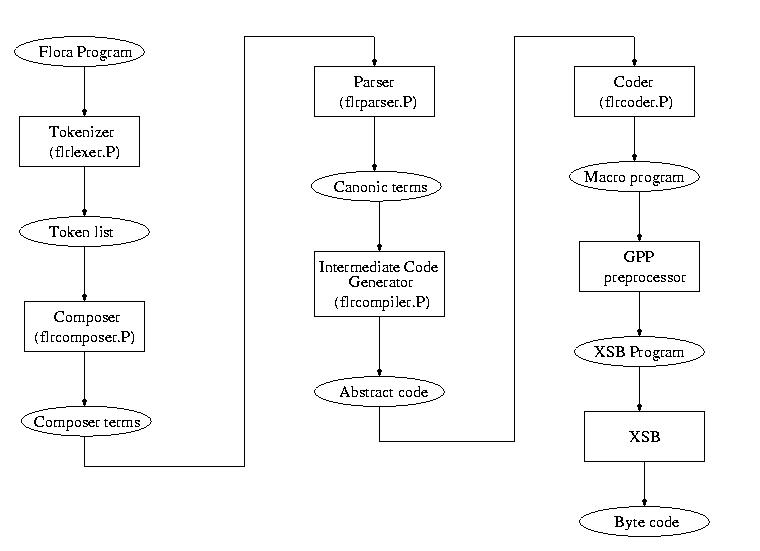
\includegraphics[width=5.5in]{architecture}
  \end{center}
  \caption{The architecture of the \FLORA system.}
  \label{fig-arch}
\end{figure}
%%

The following is a list of the key files of the system.
%%
\begin{itemize}
\item \texttt{flrshell.P}: The top level module that implements the
  \FLORA shell --- a subsystem for accepting user commands and queries and
  passing them to the compiler.  See Section~\ref{sec-shell-commands} for a
  full description of shell commands.
\item \texttt{flrlexer.P}: The \FLORA tokenizer.
\item \texttt{flrcomposer.P}: The \FLORA composer, which parses tokens
  according to the operator grammar and does other magic.
\item \texttt{flrparser.P}: The \FLORA parser.
\item \texttt{flrcompiler.P}: The generator of the intermediate code.
\item \texttt{flrcoder.P}: The \FLORA coder, which generates Prolog code.
\item \texttt{flrutils.P}: Miscellaneous utility predicates for loading
  programs, checking if files exist, whether they need to be recompiled,
  etc.
\end{itemize}
%%
Additional system libraries are located in the {\tt syslib/} subdirectory.
These include the various printing utilities, implementation for
aggregates, update primitives, and some others. The compiler determines
which of these libraries are needed while parsing the program. When a
library is needed, the compiler generates an {\tt \#include} statement to
include an appropriate file in the {\tt syslibinc} directory. For instance,
to include support for the {\tt avg} aggregate function, the compiler
copies the file {\tt syslibinc/flraggavg\_inc.flh} to the output {\tt .P}
file.  Since {\tt syslibinc/flraggavg\_inc.flh} contains the code to load
the library {\tt syslib/flraggavg.P}, this library will be loaded together
with that output file. The association between the libraries and the files
that need to be included to provide the appropriate functionality is
implemented in the file {\tt flrlibman.P}, which also implements the
utility used to load the libraries.

While {\tt syslib/} directory contains the libraries implemented in Prolog,
the {\tt lib/} directory contains libraries implemented in \FLORA itself.
Apart from that, the two types of libraries differ in functionality.  The
libraries in {\tt syslib/} implement the primitives that are part of the
syntax of the \FLORA language itself. In contrast, the libraries in {\tt
  lib/} are utilities that are part of the system, but not part of the
syntax. An example is the pretty-printing library.  Methods and predicates
defined in the libraries in {\tt lib/} are accessible through the {\tt
  @\_libname} system module and (unlike user modules) they are loaded
automatically at startup.

There are several subdirectories that hold the various files that contain
definitions included at compile time. These will be described in a
technical document.

A number of other important directories contain the various included files
(many of which include other files). The directory {\tt flrincludes/}
contains the all-important {\tt flora\_terms.flh} file, which defines all
the names used in the system. These names are defined as preprocessor
macros, so that it would be easy to change them, if necessary.
The directory {\tt genincludes/} currently contains the already mentioned
patch rules. The file {\tt flrpatch.fli} is a template, and {\tt
  flrpatch.flh}, which contains the actual patch rules, is generated from
{\tt flrpatch.fli} during installation.

The directory {\tt includes/} contains (among others) the header file,
which defines a number of important macros ({\it e.g.}, {\tt
  FLORA\_THIS\_WORKSPACE}) that wrap all the names with prefixes to
separate the different modules of the user program.  The directory {\tt
  headerinc/} is another place where the template files are located. Each
of these files contains just a few {\tt \#include} statements, mostly for
the files in the {\tt closure/} directory (which, if you recall, contains
pieces of the trailer). All meaningful combinations of these pieces of the
trailer are represented in the file {\tt includes/flrtrailer.flh}.  (Recall
that trailers implement the closure axioms.)

The directory {\tt p2h} contains (the only!) C program in the system. It
implements conversion of Prolog terms to HiLog and back. Finally, the {\tt
  pkgs/} directory is empty. Some day it will contain add-on programs, such
as Internet access, etc.


\newpage

\bibliography{flora2-manual}

\printindex

\end{document}



%%% Local Variables:
%%% mode: latex
%%% TeX-PDF-mode: t
%%% End:
